% generated from JIRA project LVV
% using template at /usr/local/lib/python3.7/site-packages/docsteady/templates/spec.latex.jinja2.
% Collecting ATM data from folder: "/Project Systems Engineering/Commissioning Science Verification"
% using docsteady version 2.0
% Please do not edit -- update information in Jira instead

\section{Test Cases Summary}\label{test-cases-summary}

\begin{longtable}[]{p{2.5cm}p{12cm}p{2cm}}
\toprule
Test Id & Test Name\tabularnewline
\midrule
\endhead
    \hyperref[lvv-t278]{LVV-T278} &
    \href{https://jira.lsstcorp.org/secure/Tests.jspa\#/testCase/LVV-T278}{Verify Out of band leakage with tunable laser and dome calibration
system} &  Defined \tabularnewline
    \hyperref[lvv-t297]{LVV-T297} &
    \href{https://jira.lsstcorp.org/secure/Tests.jspa\#/testCase/LVV-T297}{Absolute Astrometric Performance} &  Defined \tabularnewline
    \hyperref[lvv-t310]{LVV-T310} &
    \href{https://jira.lsstcorp.org/secure/Tests.jspa\#/testCase/LVV-T310}{Test cross-talk magnitudes (with CBP)} &  Defined \tabularnewline
    \hyperref[lvv-t311]{LVV-T311} &
    \href{https://jira.lsstcorp.org/secure/Tests.jspa\#/testCase/LVV-T311}{Test off-raft cross-talk limits} &  Defined \tabularnewline
    \hyperref[lvv-t312]{LVV-T312} &
    \href{https://jira.lsstcorp.org/secure/Tests.jspa\#/testCase/LVV-T312}{Test cross-talk stability and accuracy for AP, DRP} &  Defined \tabularnewline
    \hyperref[lvv-t361]{LVV-T361} &
    \href{https://jira.lsstcorp.org/secure/Tests.jspa\#/testCase/LVV-T361}{Verify 10-year Ellipticity Residuals w/ On-Sky Data} &  Defined \tabularnewline
    \hyperref[lvv-t389]{LVV-T389} &
    \href{https://jira.lsstcorp.org/secure/Tests.jspa\#/testCase/LVV-T389}{Single Visit Photometric Repeatability} &  Defined \tabularnewline
    \hyperref[lvv-t390]{LVV-T390} &
    \href{https://jira.lsstcorp.org/secure/Tests.jspa\#/testCase/LVV-T390}{The spatial uniformity of photometric zeropoints} &  Defined \tabularnewline
    \hyperref[lvv-t434]{LVV-T434} &
    \href{https://jira.lsstcorp.org/secure/Tests.jspa\#/testCase/LVV-T434}{Acquire Filter Response Verification Data (with flat field screen)} &  Defined \tabularnewline
    \hyperref[lvv-t445]{LVV-T445} &
    \href{https://jira.lsstcorp.org/secure/Tests.jspa\#/testCase/LVV-T445}{Acquire Filter Response Verification Data (with CBP)} &  Defined \tabularnewline
    \hyperref[lvv-t446]{LVV-T446} &
    \href{https://jira.lsstcorp.org/secure/Tests.jspa\#/testCase/LVV-T446}{Data Processing Campaign: Process Filter Response Verification Data
(with flat field screen)} &  Defined \tabularnewline
    \hyperref[lvv-t447]{LVV-T447} &
    \href{https://jira.lsstcorp.org/secure/Tests.jspa\#/testCase/LVV-T447}{Data Processing Campaign: Process Filter Response Verification Data
(with CBP)} &  Defined \tabularnewline
    \hyperref[lvv-t448]{LVV-T448} &
    \href{https://jira.lsstcorp.org/secure/Tests.jspa\#/testCase/LVV-T448}{Analyze Filter Response Uniformity} &  Defined \tabularnewline
    \hyperref[lvv-t450]{LVV-T450} &
    \href{https://jira.lsstcorp.org/secure/Tests.jspa\#/testCase/LVV-T450}{Science Data Pixel Noise Test \#1} &  Defined \tabularnewline
    \hyperref[lvv-t452]{LVV-T452} &
    \href{https://jira.lsstcorp.org/secure/Tests.jspa\#/testCase/LVV-T452}{Analyze in-band ripple} &  Defined \tabularnewline
    \hyperref[lvv-t453]{LVV-T453} &
    \href{https://jira.lsstcorp.org/secure/Tests.jspa\#/testCase/LVV-T453}{Analyze Filter Response Envelope} &  Defined \tabularnewline
    \hyperref[lvv-t460]{LVV-T460} &
    \href{https://jira.lsstcorp.org/secure/Tests.jspa\#/testCase/LVV-T460}{Verify Ellipticity Residuals w/ On-Sky Data for Single Exposures} &  Defined \tabularnewline
    \hyperref[lvv-t526]{LVV-T526} &
    \href{https://jira.lsstcorp.org/secure/Tests.jspa\#/testCase/LVV-T526}{Usable Pixel Fraction} &  Defined \tabularnewline
    \hyperref[lvv-t532]{LVV-T532} &
    \href{https://jira.lsstcorp.org/secure/Tests.jspa\#/testCase/LVV-T532}{MOPS completeness threshold} &  Defined \tabularnewline
    \hyperref[lvv-t543]{LVV-T543} &
    \href{https://jira.lsstcorp.org/secure/Tests.jspa\#/testCase/LVV-T543}{Astrometric error -- level 1 processing -- simulations} &  Defined \tabularnewline
    \hyperref[lvv-t544]{LVV-T544} &
    \href{https://jira.lsstcorp.org/secure/Tests.jspa\#/testCase/LVV-T544}{Astrometric error -- level 1 processing -- on-sky data} &  Defined \tabularnewline
    \hyperref[lvv-t545]{LVV-T545} &
    \href{https://jira.lsstcorp.org/secure/Tests.jspa\#/testCase/LVV-T545}{Astrometric error -- level 1 processing -- reference catalog} &  Defined \tabularnewline
    \hyperref[lvv-t546]{LVV-T546} &
    \href{https://jira.lsstcorp.org/secure/Tests.jspa\#/testCase/LVV-T546}{Photometric error -- level 1 processing -- simulations} &  Defined \tabularnewline
    \hyperref[lvv-t547]{LVV-T547} &
    \href{https://jira.lsstcorp.org/secure/Tests.jspa\#/testCase/LVV-T547}{Photometric errors -- level 1 processing -- on-sky data} &  Defined \tabularnewline
    \hyperref[lvv-t548]{LVV-T548} &
    \href{https://jira.lsstcorp.org/secure/Tests.jspa\#/testCase/LVV-T548}{Photometric errors -- level 1 processing -- reference catalog} &  Defined \tabularnewline
    \hyperref[lvv-t549]{LVV-T549} &
    \href{https://jira.lsstcorp.org/secure/Tests.jspa\#/testCase/LVV-T549}{Zeropoint consistency} &  Defined \tabularnewline
    \hyperref[lvv-t550]{LVV-T550} &
    \href{https://jira.lsstcorp.org/secure/Tests.jspa\#/testCase/LVV-T550}{MOPS -- orbit association completeness} &  Defined \tabularnewline
    \hyperref[lvv-t551]{LVV-T551} &
    \href{https://jira.lsstcorp.org/secure/Tests.jspa\#/testCase/LVV-T551}{WCS accuracy -- simulations} &  Defined \tabularnewline
    \hyperref[lvv-t554]{LVV-T554} &
    \href{https://jira.lsstcorp.org/secure/Tests.jspa\#/testCase/LVV-T554}{Single exposure dynamic range} &  Defined \tabularnewline
    \hyperref[lvv-t587]{LVV-T587} &
    \href{https://jira.lsstcorp.org/secure/Tests.jspa\#/testCase/LVV-T587}{PSF size in pixels} &  Defined \tabularnewline
    \hyperref[lvv-t588]{LVV-T588} &
    \href{https://jira.lsstcorp.org/secure/Tests.jspa\#/testCase/LVV-T588}{Median image quality at 0.44 arcsecond seeing} &  Defined \tabularnewline
    \hyperref[lvv-t589]{LVV-T589} &
    \href{https://jira.lsstcorp.org/secure/Tests.jspa\#/testCase/LVV-T589}{Median image quality at 0.6 arcsecond seeing} &  Defined \tabularnewline
    \hyperref[lvv-t590]{LVV-T590} &
    \href{https://jira.lsstcorp.org/secure/Tests.jspa\#/testCase/LVV-T590}{Median image quality at 0.8 arcsecond seeing} &  Defined \tabularnewline
    \hyperref[lvv-t591]{LVV-T591} &
    \href{https://jira.lsstcorp.org/secure/Tests.jspa\#/testCase/LVV-T591}{Flux-enclosing radius} &  Defined \tabularnewline
    \hyperref[lvv-t592]{LVV-T592} &
    \href{https://jira.lsstcorp.org/secure/Tests.jspa\#/testCase/LVV-T592}{Image quality - maximum system contribution} &  Defined \tabularnewline
    \hyperref[lvv-t593]{LVV-T593} &
    \href{https://jira.lsstcorp.org/secure/Tests.jspa\#/testCase/LVV-T593}{Image quality at zenith} &  Defined \tabularnewline
    \hyperref[lvv-t594]{LVV-T594} &
    \href{https://jira.lsstcorp.org/secure/Tests.jspa\#/testCase/LVV-T594}{Image quality - degradation from zenith} &  Defined \tabularnewline
    \hyperref[lvv-t595]{LVV-T595} &
    \href{https://jira.lsstcorp.org/secure/Tests.jspa\#/testCase/LVV-T595}{PSF ellipticity} &  Defined \tabularnewline
    \hyperref[lvv-t596]{LVV-T596} &
    \href{https://jira.lsstcorp.org/secure/Tests.jspa\#/testCase/LVV-T596}{Depth: r-band} &  Defined \tabularnewline
    \hyperref[lvv-t597]{LVV-T597} &
    \href{https://jira.lsstcorp.org/secure/Tests.jspa\#/testCase/LVV-T597}{Depth variation over field of view} &  Defined \tabularnewline
    \hyperref[lvv-t840]{LVV-T840} &
    \href{https://jira.lsstcorp.org/secure/Tests.jspa\#/testCase/LVV-T840}{Color Zeropoints} &  Defined \tabularnewline
    \hyperref[lvv-t841]{LVV-T841} &
    \href{https://jira.lsstcorp.org/secure/Tests.jspa\#/testCase/LVV-T841}{Physical Scale Transform} &  Defined \tabularnewline
    \hyperref[lvv-t853]{LVV-T853} &
    \href{https://jira.lsstcorp.org/secure/Tests.jspa\#/testCase/LVV-T853}{Resolved Source RMS} &  Defined \tabularnewline
    \hyperref[lvv-t938]{LVV-T938} &
    \href{https://jira.lsstcorp.org/secure/Tests.jspa\#/testCase/LVV-T938}{Level 2 reproducibility (same computer hardware)} &  Defined \tabularnewline
    \hyperref[lvv-t939]{LVV-T939} &
    \href{https://jira.lsstcorp.org/secure/Tests.jspa\#/testCase/LVV-T939}{Level 1 reproducibility (same computer hardware)} &  Defined \tabularnewline
    \hyperref[lvv-t940]{LVV-T940} &
    \href{https://jira.lsstcorp.org/secure/Tests.jspa\#/testCase/LVV-T940}{Level 2 reproducibility (different computer hardware)} &  Defined \tabularnewline
    \hyperref[lvv-t941]{LVV-T941} &
    \href{https://jira.lsstcorp.org/secure/Tests.jspa\#/testCase/LVV-T941}{Level 1 reproducibility (different computer hardware)} &  Defined \tabularnewline
    \hyperref[lvv-t942]{LVV-T942} &
    \href{https://jira.lsstcorp.org/secure/Tests.jspa\#/testCase/LVV-T942}{Provenance on Level 2 catalogs} &  Defined \tabularnewline
    \hyperref[lvv-t943]{LVV-T943} &
    \href{https://jira.lsstcorp.org/secure/Tests.jspa\#/testCase/LVV-T943}{Provenance in Level 1 catalogs} &  Defined \tabularnewline
    \hyperref[lvv-t950]{LVV-T950} &
    \href{https://jira.lsstcorp.org/secure/Tests.jspa\#/testCase/LVV-T950}{DIASource misassociation rate} &  Defined \tabularnewline
    \hyperref[lvv-t956]{LVV-T956} &
    \href{https://jira.lsstcorp.org/secure/Tests.jspa\#/testCase/LVV-T956}{Ghost area characterization} &  Defined \tabularnewline
    \hyperref[lvv-t957]{LVV-T957} &
    \href{https://jira.lsstcorp.org/secure/Tests.jspa\#/testCase/LVV-T957}{Ghost effect on photometric repeatability} &  Defined \tabularnewline
    \hyperref[lvv-t959]{LVV-T959} &
    \href{https://jira.lsstcorp.org/secure/Tests.jspa\#/testCase/LVV-T959}{Inter-band astrometric consistency} &  Defined \tabularnewline
    \hyperref[lvv-t960]{LVV-T960} &
    \href{https://jira.lsstcorp.org/secure/Tests.jspa\#/testCase/LVV-T960}{Relative astrometric performance (w/ Gaia)} &  Defined \tabularnewline
    \hyperref[lvv-t961]{LVV-T961} &
    \href{https://jira.lsstcorp.org/secure/Tests.jspa\#/testCase/LVV-T961}{Bright source measurement} &  Defined \tabularnewline
    \hyperref[lvv-t962]{LVV-T962} &
    \href{https://jira.lsstcorp.org/secure/Tests.jspa\#/testCase/LVV-T962}{PSF ellipticity correlations} &  Defined \tabularnewline
    \hyperref[lvv-t963]{LVV-T963} &
    \href{https://jira.lsstcorp.org/secure/Tests.jspa\#/testCase/LVV-T963}{Alert generation reliability} &  Defined \tabularnewline
    \hyperref[lvv-t964]{LVV-T964} &
    \href{https://jira.lsstcorp.org/secure/Tests.jspa\#/testCase/LVV-T964}{Quick look during outage} &  Defined \tabularnewline
    \hyperref[lvv-t965]{LVV-T965} &
    \href{https://jira.lsstcorp.org/secure/Tests.jspa\#/testCase/LVV-T965}{Sub-system health during communication outage} &  Defined \tabularnewline
    \hyperref[lvv-t966]{LVV-T966} &
    \href{https://jira.lsstcorp.org/secure/Tests.jspa\#/testCase/LVV-T966}{Image storing during outage} &  Defined \tabularnewline
    \hyperref[lvv-t967]{LVV-T967} &
    \href{https://jira.lsstcorp.org/secure/Tests.jspa\#/testCase/LVV-T967}{Scheduler functioning during communication outage} &  Defined \tabularnewline
    \hyperref[lvv-t968]{LVV-T968} &
    \href{https://jira.lsstcorp.org/secure/Tests.jspa\#/testCase/LVV-T968}{WCS measurement and reporting} &  Defined \tabularnewline
    \hyperref[lvv-t969]{LVV-T969} &
    \href{https://jira.lsstcorp.org/secure/Tests.jspa\#/testCase/LVV-T969}{Alert completeness} &  Defined \tabularnewline
    \hyperref[lvv-t986]{LVV-T986} &
    \href{https://jira.lsstcorp.org/secure/Tests.jspa\#/testCase/LVV-T986}{MOPS -- orbit association at catalog level} &  Defined \tabularnewline
    \hyperref[lvv-t999]{LVV-T999} &
    \href{https://jira.lsstcorp.org/secure/Tests.jspa\#/testCase/LVV-T999}{DM contribution to photometric error (Level 1)} &  Defined \tabularnewline
    \hyperref[lvv-t1001]{LVV-T1001} &
    \href{https://jira.lsstcorp.org/secure/Tests.jspa\#/testCase/LVV-T1001}{WCS accuracy -- on-sky data} &  Defined \tabularnewline
    \hyperref[lvv-t1002]{LVV-T1002} &
    \href{https://jira.lsstcorp.org/secure/Tests.jspa\#/testCase/LVV-T1002}{Contribution of templates to difference image noise (Mini Survey
Verification)} &  Defined \tabularnewline
    \hyperref[lvv-t1004]{LVV-T1004} &
    \href{https://jira.lsstcorp.org/secure/Tests.jspa\#/testCase/LVV-T1004}{System seeing degradation} &  Defined \tabularnewline
    \hyperref[lvv-t1006]{LVV-T1006} &
    \href{https://jira.lsstcorp.org/secure/Tests.jspa\#/testCase/LVV-T1006}{Transient completeness calculation} &  Defined \tabularnewline
    \hyperref[lvv-t1007]{LVV-T1007} &
    \href{https://jira.lsstcorp.org/secure/Tests.jspa\#/testCase/LVV-T1007}{Transient purity calculation} &  Defined \tabularnewline
    \hyperref[lvv-t1008]{LVV-T1008} &
    \href{https://jira.lsstcorp.org/secure/Tests.jspa\#/testCase/LVV-T1008}{Completeness and purity for transient sources} &  Defined \tabularnewline
    \hyperref[lvv-t1011]{LVV-T1011} &
    \href{https://jira.lsstcorp.org/secure/Tests.jspa\#/testCase/LVV-T1011}{Observatory operations during communications blackout -- 48 hours} &  Defined \tabularnewline
    \hyperref[lvv-t1012]{LVV-T1012} &
    \href{https://jira.lsstcorp.org/secure/Tests.jspa\#/testCase/LVV-T1012}{Level 2 astrometric accuracy} &  Defined \tabularnewline
    \hyperref[lvv-t1023]{LVV-T1023} &
    \href{https://jira.lsstcorp.org/secure/Tests.jspa\#/testCase/LVV-T1023}{Calibration of Atmospheric Transmission} &  Defined \tabularnewline
    \hyperref[lvv-t1029]{LVV-T1029} &
    \href{https://jira.lsstcorp.org/secure/Tests.jspa\#/testCase/LVV-T1029}{Filter Leak Constraints} &  Defined \tabularnewline
    \hyperref[lvv-t1030]{LVV-T1030} &
    \href{https://jira.lsstcorp.org/secure/Tests.jspa\#/testCase/LVV-T1030}{Zeropoint uniformity due to DM} &  Defined \tabularnewline
    \hyperref[lvv-t1031]{LVV-T1031} &
    \href{https://jira.lsstcorp.org/secure/Tests.jspa\#/testCase/LVV-T1031}{Photometric repeatability due to DM pipeline} &  Defined \tabularnewline
    \hyperref[lvv-t1032]{LVV-T1032} &
    \href{https://jira.lsstcorp.org/secure/Tests.jspa\#/testCase/LVV-T1032}{Photometric repeatability due to field of view variation} &  Defined \tabularnewline
    \hyperref[lvv-t1034]{LVV-T1034} &
    \href{https://jira.lsstcorp.org/secure/Tests.jspa\#/testCase/LVV-T1034}{Effect of gain on photometric repeatability -- 12 hours} &  Defined \tabularnewline
    \hyperref[lvv-t1035]{LVV-T1035} &
    \href{https://jira.lsstcorp.org/secure/Tests.jspa\#/testCase/LVV-T1035}{Effect of gain variations on photometric repeatability -- 1 hr} &  Defined \tabularnewline
    \hyperref[lvv-t1037]{LVV-T1037} &
    \href{https://jira.lsstcorp.org/secure/Tests.jspa\#/testCase/LVV-T1037}{Gain variation -- 1 hr} &  Defined \tabularnewline
    \hyperref[lvv-t1038]{LVV-T1038} &
    \href{https://jira.lsstcorp.org/secure/Tests.jspa\#/testCase/LVV-T1038}{Attenuation of large scale gain variation errors} &  Defined \tabularnewline
    \hyperref[lvv-t1039]{LVV-T1039} &
    \href{https://jira.lsstcorp.org/secure/Tests.jspa\#/testCase/LVV-T1039}{Attenuation of small scale gain variation over short time scales} &  Defined \tabularnewline
    \hyperref[lvv-t1040]{LVV-T1040} &
    \href{https://jira.lsstcorp.org/secure/Tests.jspa\#/testCase/LVV-T1040}{Attenuation of gain variation of an hour} &  Defined \tabularnewline
    \hyperref[lvv-t1041]{LVV-T1041} &
    \href{https://jira.lsstcorp.org/secure/Tests.jspa\#/testCase/LVV-T1041}{Stray light within 45 degrees of the moon} &  Defined \tabularnewline
    \hyperref[lvv-t1043]{LVV-T1043} &
    \href{https://jira.lsstcorp.org/secure/Tests.jspa\#/testCase/LVV-T1043}{Flat fielding errors -- effect on photometric repeatability} &  Defined \tabularnewline
    \hyperref[lvv-t1044]{LVV-T1044} &
    \href{https://jira.lsstcorp.org/secure/Tests.jspa\#/testCase/LVV-T1044}{Flat fielding -- raw effect on photometric repeatability} &  Defined \tabularnewline
    \hyperref[lvv-t1046]{LVV-T1046} &
    \href{https://jira.lsstcorp.org/secure/Tests.jspa\#/testCase/LVV-T1046}{Crosstalk functionality exists} &  Defined \tabularnewline
    \hyperref[lvv-t1048]{LVV-T1048} &
    \href{https://jira.lsstcorp.org/secure/Tests.jspa\#/testCase/LVV-T1048}{Crosstalk coefficient measurement capability} &  Defined \tabularnewline
    \hyperref[lvv-t1051]{LVV-T1051} &
    \href{https://jira.lsstcorp.org/secure/Tests.jspa\#/testCase/LVV-T1051}{color zero point accuracy due to wavelength dependent atmosphere} &  Defined \tabularnewline
    \hyperref[lvv-t1052]{LVV-T1052} &
    \href{https://jira.lsstcorp.org/secure/Tests.jspa\#/testCase/LVV-T1052}{Galaxy shape verification on recalculated deep coadds} &  Defined \tabularnewline
    \hyperref[lvv-t1053]{LVV-T1053} &
    \href{https://jira.lsstcorp.org/secure/Tests.jspa\#/testCase/LVV-T1053}{Photometric repeatability due to atmosphere calibration across the sky} &  Defined \tabularnewline
    \hyperref[lvv-t1054]{LVV-T1054} &
    \href{https://jira.lsstcorp.org/secure/Tests.jspa\#/testCase/LVV-T1054}{Photometric Calibration Uniformity due to atmosphere} &  Defined \tabularnewline
    \hyperref[lvv-t1055]{LVV-T1055} &
    \href{https://jira.lsstcorp.org/secure/Tests.jspa\#/testCase/LVV-T1055}{Maximum gray atmosphere effect} &  Defined \tabularnewline
    \hyperref[lvv-t1056]{LVV-T1056} &
    \href{https://jira.lsstcorp.org/secure/Tests.jspa\#/testCase/LVV-T1056}{Instrumental Calibration reproducibility} &  Defined \tabularnewline
    \hyperref[lvv-t1057]{LVV-T1057} &
    \href{https://jira.lsstcorp.org/secure/Tests.jspa\#/testCase/LVV-T1057}{Instrumental/System zero point uniformity} &  Defined \tabularnewline
    \hyperref[lvv-t1065]{LVV-T1065} &
    \href{https://jira.lsstcorp.org/secure/Tests.jspa\#/testCase/LVV-T1065}{Bias Image Pixel Noise Test} &  Defined \tabularnewline
    \hyperref[lvv-t1066]{LVV-T1066} &
    \href{https://jira.lsstcorp.org/secure/Tests.jspa\#/testCase/LVV-T1066}{Sky imaging test of cross-talk accuracy and stability} &  Defined \tabularnewline
    \hyperref[lvv-t1067]{LVV-T1067} &
    \href{https://jira.lsstcorp.org/secure/Tests.jspa\#/testCase/LVV-T1067}{Cross-talk significance} &  Defined \tabularnewline
    \hyperref[lvv-t1068]{LVV-T1068} &
    \href{https://jira.lsstcorp.org/secure/Tests.jspa\#/testCase/LVV-T1068}{Identification of deep image artifacts via comparison with external data
sets.} &  Defined \tabularnewline
    \hyperref[lvv-t1074]{LVV-T1074} &
    \href{https://jira.lsstcorp.org/secure/Tests.jspa\#/testCase/LVV-T1074}{Sky Brightness precision} &  Defined \tabularnewline
    \hyperref[lvv-t1075]{LVV-T1075} &
    \href{https://jira.lsstcorp.org/secure/Tests.jspa\#/testCase/LVV-T1075}{Sky Brightness Precision 2 (Simulated Data)} &  Defined \tabularnewline
    \hyperref[lvv-t1081]{LVV-T1081} &
    \href{https://jira.lsstcorp.org/secure/Tests.jspa\#/testCase/LVV-T1081}{Completeness vs. magnitude via external catalogs} &  Defined \tabularnewline
    \hyperref[lvv-t1082]{LVV-T1082} &
    \href{https://jira.lsstcorp.org/secure/Tests.jspa\#/testCase/LVV-T1082}{Completeness vs. magnitude via injected sources} &  Defined \tabularnewline
    \hyperref[lvv-t1083]{LVV-T1083} &
    \href{https://jira.lsstcorp.org/secure/Tests.jspa\#/testCase/LVV-T1083}{Single Visit Ellipticity Residuals w/ on sky data} &  Defined \tabularnewline
    \hyperref[lvv-t1084]{LVV-T1084} &
    \href{https://jira.lsstcorp.org/secure/Tests.jspa\#/testCase/LVV-T1084}{Smoothness of Rowe statistics on angular scales of 1 arcmin \textless{}
theta \textless{} 5 arcmin} &  Defined \tabularnewline
    \hyperref[lvv-t1278]{LVV-T1278} &
    \href{https://jira.lsstcorp.org/secure/Tests.jspa\#/testCase/LVV-T1278}{Relative Astrometric Performance (Repeatability)} &  Defined \tabularnewline
    \hyperref[lvv-t293]{LVV-T293} &
    \href{https://jira.lsstcorp.org/secure/Tests.jspa\#/testCase/LVV-T293}{On-sky Observations: Single-visit Key Performance Metrics} &  Draft \tabularnewline
    \hyperref[lvv-t294]{LVV-T294} &
    \href{https://jira.lsstcorp.org/secure/Tests.jspa\#/testCase/LVV-T294}{On-sky Observations: Full-survey Key Performance Metrics} &  Draft \tabularnewline
    \hyperref[lvv-t295]{LVV-T295} &
    \href{https://jira.lsstcorp.org/secure/Tests.jspa\#/testCase/LVV-T295}{Data Processing Campaign: Single-visit Key Performance Metrics} &  Draft \tabularnewline
    \hyperref[lvv-t296]{LVV-T296} &
    \href{https://jira.lsstcorp.org/secure/Tests.jspa\#/testCase/LVV-T296}{Data Processing Campaign: Full-survey Key Performance Metrics} &  Draft \tabularnewline
    \hyperref[lvv-t298]{LVV-T298} &
    \href{https://jira.lsstcorp.org/secure/Tests.jspa\#/testCase/LVV-T298}{Cross-band Astrometric Performance} &  Draft \tabularnewline
    \hyperref[lvv-t299]{LVV-T299} &
    \href{https://jira.lsstcorp.org/secure/Tests.jspa\#/testCase/LVV-T299}{Relative Astrometric Performance} &  Draft \tabularnewline
    \hyperref[lvv-t360]{LVV-T360} &
    \href{https://jira.lsstcorp.org/secure/Tests.jspa\#/testCase/LVV-T360}{Off Zenith Image Quality Degradation} &  Draft \tabularnewline
    \hyperref[lvv-t442]{LVV-T442} &
    \href{https://jira.lsstcorp.org/secure/Tests.jspa\#/testCase/LVV-T442}{Control Ghosts in Coadds} &  Draft \tabularnewline
    \hyperref[lvv-t461]{LVV-T461} &
    \href{https://jira.lsstcorp.org/secure/Tests.jspa\#/testCase/LVV-T461}{Filter Out of Band Constraints} &  Draft \tabularnewline
    \hyperref[lvv-t533]{LVV-T533} &
    \href{https://jira.lsstcorp.org/secure/Tests.jspa\#/testCase/LVV-T533}{MOPS purity threshold} &  Draft \tabularnewline
    \hyperref[lvv-t975]{LVV-T975} &
    \href{https://jira.lsstcorp.org/secure/Tests.jspa\#/testCase/LVV-T975}{Process ComCam images -- DRP} &  Draft \tabularnewline
    \hyperref[lvv-t976]{LVV-T976} &
    \href{https://jira.lsstcorp.org/secure/Tests.jspa\#/testCase/LVV-T976}{Process ComCam images -- AP} &  Draft \tabularnewline
    \hyperref[lvv-t979]{LVV-T979} &
    \href{https://jira.lsstcorp.org/secure/Tests.jspa\#/testCase/LVV-T979}{Mini-survey 2 -- DRP test} &  Draft \tabularnewline
    \hyperref[lvv-t1033]{LVV-T1033} &
    \href{https://jira.lsstcorp.org/secure/Tests.jspa\#/testCase/LVV-T1033}{Generate grid of sources with CBP} &  Draft \tabularnewline
    \hyperref[lvv-t1070]{LVV-T1070} &
    \href{https://jira.lsstcorp.org/secure/Tests.jspa\#/testCase/LVV-T1070}{On-sky Observations: 10-year Depth SV Survey} &  Draft \tabularnewline
    \hyperref[lvv-t1071]{LVV-T1071} &
    \href{https://jira.lsstcorp.org/secure/Tests.jspa\#/testCase/LVV-T1071}{On-sky Observations: 20-year Depth Test} &  Draft \tabularnewline
    \hyperref[lvv-t1072]{LVV-T1072} &
    \href{https://jira.lsstcorp.org/secure/Tests.jspa\#/testCase/LVV-T1072}{Data Processing Campaign: Data Release Processing} &  Draft \tabularnewline
    \hyperref[lvv-t1073]{LVV-T1073} &
    \href{https://jira.lsstcorp.org/secure/Tests.jspa\#/testCase/LVV-T1073}{On-sky Observations: Wide-area SV Survey} &  Draft \tabularnewline
\bottomrule
\end{longtable}

\newpage

\section{Active Test Cases}

This section documents all active test cases that have a status in the Jira/ATM system of Draft, Defined or Approved.

\subsection{ Defined Test Cases}

\subsubsection{LVV-T278 - Verify Out of band leakage with tunable laser and dome calibration
system}\label{lvv-t278}

\begin{longtable}[]{llllll}
\toprule
Version & Status & Priority & Verification Type & Owner
\\\midrule
1 & Defined & Normal &
Test & Craig Lage
\\\bottomrule
\multicolumn{6}{c}{ Open \href{https://jira.lsstcorp.org/secure/Tests.jspa\#/testCase/LVV-T278}{LVV-T278} in Jira } \\
\end{longtable}

\paragraph{Verification Elements}\mbox{}\\

\begin{itemize}
\item \href{https://jira.lsstcorp.org/browse/LVV-790}{LVV-790} - OSS-REQ-0237-V-01: Filter Out of Band Constraints

\end{itemize}

\paragraph{Test Items}\mbox{}\\

Out of band leakage meets spec.








\paragraph{Test Procedure}\mbox{}\\
\begin{tabular}{p{4cm}p{12cm}}
\toprule
Step 1
& Description \\ \hline
\end{tabular}
{\scriptsize
Choose 1 one of the 6 filters

}
\begin{tabular}{p{3cm}p{13cm}}
\hline
            & Expected Result \\ \hline
\end{tabular}

\begin{tabular}{p{4cm}p{12cm}}
\toprule
Step 2
& Description \\ \hline
\end{tabular}
{\scriptsize
Scan the tunable laser from 300nm to 1200nm.~ For each increment, take
an exposure. Use the DM software to perform the Instrument Signature
Removal. ~Then take the median intensity for each CCD in the focal
plane.

}
\begin{tabular}{p{3cm}p{13cm}}
\hline
            & Test Data \\ \hline
\end{tabular}
{\scriptsize
Full focal plane flat field images.

}
\begin{tabular}{p{3cm}p{13cm}}
\hline
            & Expected Result \\ \hline
\end{tabular}
{\scriptsize
(1) If the tunable laser is within the filter bandpass, measure the
intensity at the central wavelength. Call this intensity I0.\\
(2) If the tunable laser wavelength is outside of one FWHM from the
central wavelength of the filter, the image intensity should meet the
following criteria:\\
\hspace*{0.333em} ~ ~(A) The average leakage in any 10nm segment between
300- 1200nm outside the wavelength span one FWHM should not exceed
0.01\% of I0.\\
\hspace*{0.333em} ~ ~(B) The number of these out-of-band measurements
which are between 0.01\% and 0.1\% of I0 must be less than 1/20 of the
total number of out-of-band measurements.\\
(3) The integrated transmission over all wavelengths between 300-1200nm
outside the wavelength span ~between the first time the filter response
goes below 0.1\% of the peak the total shall not exceeded 0.03\%
relative to the total integrated transmission between 300nm and
1200nm.\\
(4) The maximum leakage should not exceed 0.1\% of 10.\\
(5) Repeat for all filters.\\[4\baselineskip]

}

\begin{tabular}{p{4cm}p{12cm}}
\toprule
Step 3
& Description \\ \hline
\end{tabular}
{\scriptsize
Repeat the above for each of the 6 filters.\\[2\baselineskip]

}
\begin{tabular}{p{3cm}p{13cm}}
\hline
            & Expected Result \\ \hline
\end{tabular}

\subsubsection{LVV-T297 - Absolute Astrometric Performance}\label{lvv-t297}

\begin{longtable}[]{llllll}
\toprule
Version & Status & Priority & Verification Type & Owner
\\\midrule
1 & Defined & Normal &
Test & Keith Bechtol
\\\bottomrule
\multicolumn{6}{c}{ Open \href{https://jira.lsstcorp.org/secure/Tests.jspa\#/testCase/LVV-T297}{LVV-T297} in Jira } \\
\end{longtable}

\paragraph{Verification Elements}\mbox{}\\

\begin{itemize}
\item \href{https://jira.lsstcorp.org/browse/LVV-238}{LVV-238} - LSR-REQ-0094-V-01: Astrometric Performance1

\item \href{https://jira.lsstcorp.org/browse/LVV-1544}{LVV-1544} - OSS-REQ-0228-V-02: Image Size in Pixels

\item \href{https://jira.lsstcorp.org/browse/LVV-1273}{LVV-1273} - OSS-REQ-0149-V-01: Level 1 Catalog Precision

\item \href{https://jira.lsstcorp.org/browse/LVV-1363}{LVV-1363} - OSS-REQ-0388-V-01: Astrometric Performance

\end{itemize}

\paragraph{Test Items}\mbox{}\\

Measure astrometric performance using Gaia as an external reference.








\paragraph{Test Procedure}\mbox{}\\
\begin{tabular}{p{4cm}p{12cm}}
\toprule
Step 1
& Description \\ \hline
\end{tabular}
{\scriptsize
Take images from region overlapping the Gaia footprint. ~Repeat at
multiple airmasses.

}
\begin{tabular}{p{3cm}p{13cm}}
\hline
            & Expected Result \\ \hline
\end{tabular}
{\scriptsize
Set of images

}

\begin{tabular}{p{4cm}p{12cm}}
\toprule
Step 2
& Description \\ \hline
\end{tabular}
{\scriptsize
Perform source detection and astrometric measurement on images from step
1

}
\begin{tabular}{p{3cm}p{13cm}}
\hline
            & Test Data \\ \hline
\end{tabular}
{\scriptsize
Images from step 1

}
\begin{tabular}{p{3cm}p{13cm}}
\hline
            & Expected Result \\ \hline
\end{tabular}
{\scriptsize
Catalog of sources

}

\begin{tabular}{p{4cm}p{12cm}}
\toprule
Step 3
& Description \\ \hline
\end{tabular}
{\scriptsize
Cross-match catalog from step 2 with Gaia catalog. ~Select sources that
are consistent with zero proper motion (according to Gaia).

}
\begin{tabular}{p{3cm}p{13cm}}
\hline
            & Test Data \\ \hline
\end{tabular}
{\scriptsize
Catalog of sources from step 2\\
Catalog of Gaia sources with measured positions

}
\begin{tabular}{p{3cm}p{13cm}}
\hline
            & Expected Result \\ \hline
\end{tabular}
{\scriptsize
Cross-matched catalog of sources seen by both LSST and Gaia

}

\begin{tabular}{p{4cm}p{12cm}}
\toprule
Step 4
& Description \\ \hline
\end{tabular}
{\scriptsize
Verify that the median error of the LSST positions (relative to the Gaia
positions) is 50 milliarcseconds in RA, Dec independently

}
\begin{tabular}{p{3cm}p{13cm}}
\hline
            & Test Data \\ \hline
\end{tabular}
{\scriptsize
Cross-matched catalog from step 3

}
\begin{tabular}{p{3cm}p{13cm}}
\hline
            & Expected Result \\ \hline
\end{tabular}

\subsubsection{LVV-T310 - Test cross-talk magnitudes (with CBP)}\label{lvv-t310}

\begin{longtable}[]{llllll}
\toprule
Version & Status & Priority & Verification Type & Owner
\\\midrule
1 & Defined & Normal &
Test & Brian Stalder
\\\bottomrule
\multicolumn{6}{c}{ Open \href{https://jira.lsstcorp.org/secure/Tests.jspa\#/testCase/LVV-T310}{LVV-T310} in Jira } \\
\end{longtable}

\paragraph{Verification Elements}\mbox{}\\

\begin{itemize}
\item \href{https://jira.lsstcorp.org/browse/LVV-1633}{LVV-1633} - OSS-REQ-0327-V-01: Crosstalk Magnitude Limits

\end{itemize}

\paragraph{Test Items}\mbox{}\\

verify cross-talk terms are within limits








\paragraph{Test Procedure}\mbox{}\\
\begin{tabular}{p{4cm}p{12cm}}
\toprule
Step 1
& Description \\ \hline
\end{tabular}
{\scriptsize
take cross-talk test image

}
\begin{tabular}{p{3cm}p{13cm}}
\hline
            & Expected Result \\ \hline
\end{tabular}

\begin{tabular}{p{4cm}p{12cm}}
\toprule
Step 2
& Description \\ \hline
\end{tabular}
{\scriptsize
run through calibration products pipeline

}
\begin{tabular}{p{3cm}p{13cm}}
\hline
            & Expected Result \\ \hline
\end{tabular}

\begin{tabular}{p{4cm}p{12cm}}
\toprule
Step 3
& Description \\ \hline
\end{tabular}
{\scriptsize
retrieve cross-talk terms

}
\begin{tabular}{p{3cm}p{13cm}}
\hline
            & Expected Result \\ \hline
\end{tabular}

\begin{tabular}{p{4cm}p{12cm}}
\toprule
Step 4
& Description \\ \hline
\end{tabular}
{\scriptsize
compare resultant matrix elements are within required limits

}
\begin{tabular}{p{3cm}p{13cm}}
\hline
            & Expected Result \\ \hline
\end{tabular}

\subsubsection{LVV-T311 - Test off-raft cross-talk limits}\label{lvv-t311}

\begin{longtable}[]{llllll}
\toprule
Version & Status & Priority & Verification Type & Owner
\\\midrule
1 & Defined & Normal &
Test & Brian Stalder
\\\bottomrule
\multicolumn{6}{c}{ Open \href{https://jira.lsstcorp.org/secure/Tests.jspa\#/testCase/LVV-T311}{LVV-T311} in Jira } \\
\end{longtable}

\paragraph{Verification Elements}\mbox{}\\

\begin{itemize}
\item \href{https://jira.lsstcorp.org/browse/LVV-1627}{LVV-1627} - OSS-REQ-0328-V-01: Crosstalk Aggressor Limits

\end{itemize}

\paragraph{Test Items}\mbox{}\\

verify that off-raft contributed cross-talk is below limits








\paragraph{Test Procedure}\mbox{}\\
\begin{tabular}{p{4cm}p{12cm}}
\toprule
Step 1
& Description \\ \hline
\end{tabular}
{\scriptsize
take cross-talk test image

}
\begin{tabular}{p{3cm}p{13cm}}
\hline
            & Expected Result \\ \hline
\end{tabular}

\begin{tabular}{p{4cm}p{12cm}}
\toprule
Step 2
& Description \\ \hline
\end{tabular}
{\scriptsize
process through calibrated products pipeline

}
\begin{tabular}{p{3cm}p{13cm}}
\hline
            & Expected Result \\ \hline
\end{tabular}

\begin{tabular}{p{4cm}p{12cm}}
\toprule
Step 3
& Description \\ \hline
\end{tabular}
{\scriptsize
retrieve cross-talk matrix, verify off-raft elements are within required
limits

}
\begin{tabular}{p{3cm}p{13cm}}
\hline
            & Expected Result \\ \hline
\end{tabular}

\subsubsection{LVV-T312 - Test cross-talk stability and accuracy for AP, DRP}\label{lvv-t312}

\begin{longtable}[]{llllll}
\toprule
Version & Status & Priority & Verification Type & Owner
\\\midrule
1 & Defined & Normal &
Test & Brian Stalder
\\\bottomrule
\multicolumn{6}{c}{ Open \href{https://jira.lsstcorp.org/secure/Tests.jspa\#/testCase/LVV-T312}{LVV-T312} in Jira } \\
\end{longtable}

\paragraph{Verification Elements}\mbox{}\\

\begin{itemize}
\item \href{https://jira.lsstcorp.org/browse/LVV-1624}{LVV-1624} - OSS-REQ-0329-V-01: Crosstalk Accuracy

\end{itemize}

\paragraph{Test Items}\mbox{}\\

verify stability and accuracy of cross-talk elements for AP and DRP
production (if different)~








\paragraph{Test Procedure}\mbox{}\\
\begin{tabular}{p{4cm}p{12cm}}
\toprule
Step 1
& Description \\ \hline
\end{tabular}
{\scriptsize
take series of cross-talk test images over a long
(\textgreater{}=required) baseline

}
\begin{tabular}{p{3cm}p{13cm}}
\hline
            & Expected Result \\ \hline
\end{tabular}

\begin{tabular}{p{4cm}p{12cm}}
\toprule
Step 2
& Description \\ \hline
\end{tabular}
{\scriptsize
run through calibration products pipeline (for AP and DRP).

}
\begin{tabular}{p{3cm}p{13cm}}
\hline
            & Expected Result \\ \hline
\end{tabular}

\begin{tabular}{p{4cm}p{12cm}}
\toprule
Step 3
& Description \\ \hline
\end{tabular}
{\scriptsize
retrieve cross-talk matrix and verify RMS stability over baseline is
below accuracy limits for AP and DRP, depending on algorithm used. Focus
on inter-amplifier cross-talk, where we know the cross-talk is largest.

}
\begin{tabular}{p{3cm}p{13cm}}
\hline
            & Expected Result \\ \hline
\end{tabular}

\subsubsection{LVV-T361 - Verify 10-year Ellipticity Residuals w/ On-Sky Data}\label{lvv-t361}

\begin{longtable}[]{llllll}
\toprule
Version & Status & Priority & Verification Type & Owner
\\\midrule
1 & Defined & Normal &
Analysis & Keith Bechtol
\\\bottomrule
\multicolumn{6}{c}{ Open \href{https://jira.lsstcorp.org/secure/Tests.jspa\#/testCase/LVV-T361}{LVV-T361} in Jira } \\
\end{longtable}

\paragraph{Verification Elements}\mbox{}\\

\begin{itemize}
\item \href{https://jira.lsstcorp.org/browse/LVV-1546}{LVV-1546} - OSS-REQ-0234-V-01: 10-year Ellipticity Residuals

\item \href{https://jira.lsstcorp.org/browse/LVV-1366}{LVV-1366} - OSS-REQ-0390-V-01: Ellipticity Correlations

\end{itemize}

\paragraph{Test Items}\mbox{}\\

This is closely related to DMS-REQ-0362. It is likely that we can
recycle some parts of analysis code.








\paragraph{Test Procedure}\mbox{}\\
\begin{tabular}{p{4cm}p{12cm}}
\toprule
Step 1
& Description \\ \hline
\end{tabular}
{\scriptsize
Point the butler to the deep coadd repo, to extract the CoaddPsf, and
deep coadd catalogs.

}
\begin{tabular}{p{3cm}p{13cm}}
\hline
            & Expected Result \\ \hline
\end{tabular}

\begin{tabular}{p{4cm}p{12cm}}
\toprule
Step 2
& Description \\ \hline
\end{tabular}
{\scriptsize
Obtain deep ~catalogs whose deep coadds of a contiguous representative
piece on scale necessary to satisfy the residual correlations we will
examine for this test.

}
\begin{tabular}{p{3cm}p{13cm}}
\hline
            & Expected Result \\ \hline
\end{tabular}

\begin{tabular}{p{4cm}p{12cm}}
\toprule
Step 3
& Description \\ \hline
\end{tabular}
{\scriptsize
Consider separately stars that were included in PSF modeling and stars
that were not included in PSF modeling. The fiduciual result for this
test should use the stars that were not included in PSF modeling. The
stars that were included in PSF modeling will still be useful for
diagnostic purposes.

}
\begin{tabular}{p{3cm}p{13cm}}
\hline
            & Expected Result \\ \hline
\end{tabular}

\begin{tabular}{p{4cm}p{12cm}}
\toprule
Step 4
& Description \\ \hline
\end{tabular}
{\scriptsize
For each stellar sample, compute all Rowe statistics over angular scales
ranging from less than 1 arcmin to greater than 5
arcmin.\\[2\baselineskip]This will require the CoaddPsf model for
calculating residuals. To calculate residuals, obtain the CoaddPsf model
evaluated at the positions of stars of interest, and find the difference
in the measured ellipticity of stars, and the model ellipticity.

}
\begin{tabular}{p{3cm}p{13cm}}
\hline
            & Expected Result \\ \hline
\end{tabular}

\begin{tabular}{p{4cm}p{12cm}}
\toprule
Step 5
& Description \\ \hline
\end{tabular}
{\scriptsize
Extract the amplitudes of the Rowe statistics at angular scales of 1
arcmin and less, and 5 arcmin and larger

}
\begin{tabular}{p{3cm}p{13cm}}
\hline
            & Expected Result \\ \hline
\end{tabular}

\begin{tabular}{p{4cm}p{12cm}}
\toprule
Step 6
& Description \\ \hline
\end{tabular}
{\scriptsize
For each angular scale (\textless{}1 arcmin and \textgreater{}5 arcmin),
for each Rowe statistic, collect the amplitudes of the Rowe statistics.

}
\begin{tabular}{p{3cm}p{13cm}}
\hline
            & Expected Result \\ \hline
\end{tabular}

\begin{tabular}{p{4cm}p{12cm}}
\toprule
Step 7
& Description \\ \hline
\end{tabular}
{\scriptsize
Calculate the medians from the amplitudes corresponding to each angular
scale, for each Rowe statistic.

}
\begin{tabular}{p{3cm}p{13cm}}
\hline
            & Expected Result \\ \hline
\end{tabular}

\begin{tabular}{p{4cm}p{12cm}}
\toprule
Step 8
& Description \\ \hline
\end{tabular}
{\scriptsize
Confirm that the medians are within the specifications

}
\begin{tabular}{p{3cm}p{13cm}}
\hline
            & Expected Result \\ \hline
\end{tabular}

\begin{tabular}{p{4cm}p{12cm}}
\toprule
Step 9
& Description \\ \hline
\end{tabular}
{\scriptsize
Confirm that the Rowe statistics are smooth through 1 arcmin to 5 arcmin

}
\begin{tabular}{p{3cm}p{13cm}}
\hline
            & Expected Result \\ \hline
\end{tabular}

\subsubsection{LVV-T389 - Single Visit Photometric Repeatability}\label{lvv-t389}

\begin{longtable}[]{llllll}
\toprule
Version & Status & Priority & Verification Type & Owner
\\\midrule
1 & Defined & Normal &
Analysis & Imram Hasan
\\\bottomrule
\multicolumn{6}{c}{ Open \href{https://jira.lsstcorp.org/secure/Tests.jspa\#/testCase/LVV-T389}{LVV-T389} in Jira } \\
\end{longtable}

\paragraph{Verification Elements}\mbox{}\\

\begin{itemize}
\item \href{https://jira.lsstcorp.org/browse/LVV-273}{LVV-273} - LSR-REQ-0093-V-01: Photometric Performance1

\item \href{https://jira.lsstcorp.org/browse/LVV-1372}{LVV-1372} - OSS-REQ-0387-V-01: Single visit photometric repeatability

\end{itemize}

\paragraph{Test Items}\mbox{}\\

Verify that the RMS of magnitudes in all filters and outlier rate of
magnitudes is within specification








\paragraph{Test Procedure}\mbox{}\\
\begin{tabular}{p{4cm}p{12cm}}
\toprule
Step 1
& Description \\ \hline
\end{tabular}
{\scriptsize
Define sample data of stars to be used in subsequent tests. ~Columns
needed are camera rotation angle, magnitude in all bands, RA, Dec,
detector position.

}
\begin{tabular}{p{3cm}p{13cm}}
\hline
            & Test Data \\ \hline
\end{tabular}
{\scriptsize
LSST Photometry from main sequence, variable, bright, non-saturated
non-resolved point sources. Observations need to span sky position,
camera position, chip position, object color, brightness, airmass, water
vapor content, and time of observation.\\[2\baselineskip]Per The LSST
SRD, bright means 1-4 magnitudes fainter than saturation
limits.\\[2\baselineskip]We estimate this will require at
\textasciitilde{} 50,000 objects in order to overcome statistical noise.
This will require about 50**2 degrees of imaging, assuming there are
1000 stars per square degree. This roughly corresponds to
\textasciitilde{}100 ComCam pointing.~

}
\begin{tabular}{p{3cm}p{13cm}}
\hline
            & Expected Result \\ \hline
\end{tabular}

\begin{tabular}{p{4cm}p{12cm}}
\toprule
Step 2
& Description \\ \hline
\end{tabular}
{\scriptsize
For each star, measure the RMS magnitude in each filter. This yields a
distribution of RMS values in each filter. Calculate the median of the
distributions for each filter.

}
\begin{tabular}{p{3cm}p{13cm}}
\hline
            & Expected Result \\ \hline
\end{tabular}

\begin{tabular}{p{4cm}p{12cm}}
\toprule
Step 3
& Description \\ \hline
\end{tabular}
{\scriptsize
For each star, calculate the mean magnitude. Calculate the number of
observations which deviate by more than PA2gri (15) millimags from their
means for magnitudes in the g, r, and i bands and PA2uzy (22.5)
millimags ~for magnitudes in the u, z, and y bands.

}
\begin{tabular}{p{3cm}p{13cm}}
\hline
            & Expected Result \\ \hline
\end{tabular}

\begin{tabular}{p{4cm}p{12cm}}
\toprule
Step 4
& Description \\ \hline
\end{tabular}
{\scriptsize
Check the median RMS values for u, z, ~are below PA1uzy (7.5)
millimagniutes

}
\begin{tabular}{p{3cm}p{13cm}}
\hline
            & Expected Result \\ \hline
\end{tabular}

\begin{tabular}{p{4cm}p{12cm}}
\toprule
Step 5
& Description \\ \hline
\end{tabular}
{\scriptsize
Check the median RMS values for g, r, i are below PA1gri (5)
millimagnitudes~

}
\begin{tabular}{p{3cm}p{13cm}}
\hline
            & Expected Result \\ \hline
\end{tabular}

\begin{tabular}{p{4cm}p{12cm}}
\toprule
Step 6
& Description \\ \hline
\end{tabular}
{\scriptsize
Check that less than PF1 (10\%) of measurements deviate from their means
by more than PA2 from step 3

}
\begin{tabular}{p{3cm}p{13cm}}
\hline
            & Expected Result \\ \hline
\end{tabular}

\subsubsection{LVV-T390 - The spatial uniformity of photometric zeropoints}\label{lvv-t390}

\begin{longtable}[]{llllll}
\toprule
Version & Status & Priority & Verification Type & Owner
\\\midrule
1 & Defined & Normal &
Analysis & Sam Schmidt
\\\bottomrule
\multicolumn{6}{c}{ Open \href{https://jira.lsstcorp.org/secure/Tests.jspa\#/testCase/LVV-T390}{LVV-T390} in Jira } \\
\end{longtable}

\paragraph{Verification Elements}\mbox{}\\

\begin{itemize}
\item \href{https://jira.lsstcorp.org/browse/LVV-274}{LVV-274} - LSR-REQ-0093-V-02: Photometric Performance2

\item \href{https://jira.lsstcorp.org/browse/LVV-1373}{LVV-1373} - OSS-REQ-0387-V-02: Zero point spatial uniformity

\end{itemize}

\paragraph{Test Items}\mbox{}\\

The distribution width (rms) of the internal photometric zero-point
error (the system stability across the sky) will not exceed PA3/PA3u
millimag, and no more than PF2 \% of the distribution will exceed PF4
millimag. ~Applies to both bright and faint ends to constrain
non-linearity of the flux scale








\paragraph{Test Procedure}\mbox{}\\
\begin{tabular}{p{4cm}p{12cm}}
\toprule
Step 1
& Description \\ \hline
\end{tabular}
{\scriptsize
Identify fields spread across the sky with available
(spectrophotometric?) standard stars so that zero points can be
determined. ~Reserve some portion of the standard stars to test that are
not used in determining the zero point. ~Alternatively, identify
specific marker points in color-color diagrams that can be used to
define relative zero point offsets. ~Requires both bright and faint
samples.

}
\begin{tabular}{p{3cm}p{13cm}}
\hline
            & Test Data \\ \hline
\end{tabular}
{\scriptsize
Columns needed: RA, DEC; x, y position on focal plane; magnitudes in all
six ugrizy bands

}
\begin{tabular}{p{3cm}p{13cm}}
\hline
            & Expected Result \\ \hline
\end{tabular}

\begin{tabular}{p{4cm}p{12cm}}
\toprule
Step 2
& Description \\ \hline
\end{tabular}
{\scriptsize
Run DMstack, which determines photometric zero points for stars for each
patch of the sky

}
\begin{tabular}{p{3cm}p{13cm}}
\hline
            & Test Data \\ \hline
\end{tabular}
{\scriptsize
data from step 1

}
\begin{tabular}{p{3cm}p{13cm}}
\hline
            & Expected Result \\ \hline
\end{tabular}

\begin{tabular}{p{4cm}p{12cm}}
\toprule
Step 3
& Description \\ \hline
\end{tabular}
{\scriptsize
For test stars reserved and not used in zero point determination,
calculate RMS of differences between measured and standard star
magnitudes. Check that RMS is less than PA3u (20 mmag) in the u-band,
and less than PA3 (10 mmag) for grizy bands.

}
\begin{tabular}{p{3cm}p{13cm}}
\hline
            & Test Data \\ \hline
\end{tabular}
{\scriptsize
zero points from step 2

}
\begin{tabular}{p{3cm}p{13cm}}
\hline
            & Expected Result \\ \hline
\end{tabular}

\begin{tabular}{p{4cm}p{12cm}}
\toprule
Step 4
& Description \\ \hline
\end{tabular}
{\scriptsize
Check that no more than PF2 percent (10\%) of the magnitude differences
exceed a difference of PF4 (15 mmag)

}
\begin{tabular}{p{3cm}p{13cm}}
\hline
            & Test Data \\ \hline
\end{tabular}
{\scriptsize
zero points from step 2

}
\begin{tabular}{p{3cm}p{13cm}}
\hline
            & Expected Result \\ \hline
\end{tabular}

\subsubsection{LVV-T434 - Acquire Filter Response Verification Data (with flat field screen)}\label{lvv-t434}

\begin{longtable}[]{llllll}
\toprule
Version & Status & Priority & Verification Type & Owner
\\\midrule
1 & Defined & Normal &
Test & Brian Stalder
\\\bottomrule
\multicolumn{6}{c}{ Open \href{https://jira.lsstcorp.org/secure/Tests.jspa\#/testCase/LVV-T434}{LVV-T434} in Jira } \\
\end{longtable}

\paragraph{Verification Elements}\mbox{}\\

\begin{itemize}
\item \href{https://jira.lsstcorp.org/browse/LVV-1555}{LVV-1555} - OSS-REQ-0238-V-01: Filter Response Uniformity u-band blue edge

\item \href{https://jira.lsstcorp.org/browse/LVV-1570}{LVV-1570} - OSS-REQ-0239-V-01: In-band Ripple u-band

\item \href{https://jira.lsstcorp.org/browse/LVV-1582}{LVV-1582} - OSS-REQ-0240-V-01: u-band Response Envelope

\item \href{https://jira.lsstcorp.org/browse/LVV-1579}{LVV-1579} - OSS-REQ-0366-V-01: u-band not-to-exceed envelope

\item \href{https://jira.lsstcorp.org/browse/LVV-1561}{LVV-1561} - OSS-REQ-0241-V-01: g-band Response Envelope

\item \href{https://jira.lsstcorp.org/browse/LVV-1558}{LVV-1558} - OSS-REQ-0367-V-01: g-band not-to-exceed envelope

\item \href{https://jira.lsstcorp.org/browse/LVV-1576}{LVV-1576} - OSS-REQ-0242-V-01: r-band Response Envelope

\item \href{https://jira.lsstcorp.org/browse/LVV-1573}{LVV-1573} - OSS-REQ-0368-V-01: r-band not-to-exceed envelope

\item \href{https://jira.lsstcorp.org/browse/LVV-1567}{LVV-1567} - OSS-REQ-0243-V-01: i-band Response Envelope

\item \href{https://jira.lsstcorp.org/browse/LVV-1564}{LVV-1564} - OSS-REQ-0369-V-01: i-band not-to-exceed envelope

\item \href{https://jira.lsstcorp.org/browse/LVV-1594}{LVV-1594} - OSS-REQ-0244-V-01: z-band Response Envelope

\item \href{https://jira.lsstcorp.org/browse/LVV-1591}{LVV-1591} - OSS-REQ-0370-V-01: z-band not-to-exceed envelope

\item \href{https://jira.lsstcorp.org/browse/LVV-1588}{LVV-1588} - OSS-REQ-0245-V-01: y-band Response Envelope

\item \href{https://jira.lsstcorp.org/browse/LVV-1585}{LVV-1585} - OSS-REQ-0371-V-01: y-band not-to-exceed envelope

\item \href{https://jira.lsstcorp.org/browse/LVV-1556}{LVV-1556} - OSS-REQ-0238-V-02: Filter Response Uniformity u-band red edge

\item \href{https://jira.lsstcorp.org/browse/LVV-1557}{LVV-1557} - OSS-REQ-0238-V-03: Filter Response Uniformity g-band blue edge

\item \href{https://jira.lsstcorp.org/browse/LVV-8678}{LVV-8678} - OSS-REQ-0238-V-04: Filter Response Uniformity g-band red edge

\item \href{https://jira.lsstcorp.org/browse/LVV-8681}{LVV-8681} - OSS-REQ-0238-V-05: Filter Response Uniformity r-band blue edge

\item \href{https://jira.lsstcorp.org/browse/LVV-8683}{LVV-8683} - OSS-REQ-0238-V-06: Filter Response Uniformity r-band red edge

\item \href{https://jira.lsstcorp.org/browse/LVV-8686}{LVV-8686} - OSS-REQ-0238-V-07: Filter Response Uniformity i-band blue edge

\item \href{https://jira.lsstcorp.org/browse/LVV-8689}{LVV-8689} - OSS-REQ-0238-V-08: Filter Response Uniformity i-band red edge

\item \href{https://jira.lsstcorp.org/browse/LVV-8691}{LVV-8691} - OSS-REQ-0238-V-09: Filter Response Uniformity z-band blue edge

\item \href{https://jira.lsstcorp.org/browse/LVV-8694}{LVV-8694} - OSS-REQ-0238-V-10: Filter Response Uniformity z-band red edge

\item \href{https://jira.lsstcorp.org/browse/LVV-8696}{LVV-8696} - OSS-REQ-0238-V-11: Filter Response Uniformity y-band blue edge

\item \href{https://jira.lsstcorp.org/browse/LVV-8698}{LVV-8698} - OSS-REQ-0238-V-12: Filter Response Uniformity y-band red edge

\item \href{https://jira.lsstcorp.org/browse/LVV-1572}{LVV-1572} - OSS-REQ-0239-V-03: In-band Ripple r-band

\item \href{https://jira.lsstcorp.org/browse/LVV-1571}{LVV-1571} - OSS-REQ-0239-V-02: In-band Ripple g-band

\item \href{https://jira.lsstcorp.org/browse/LVV-790}{LVV-790} - OSS-REQ-0237-V-01: Filter Out of Band Constraints

\end{itemize}

\paragraph{Test Items}\mbox{}\\









\paragraph{Test Procedure}\mbox{}\\
\begin{tabular}{p{4cm}p{12cm}}
\toprule
Step 1
& Description \\ \hline
\end{tabular}
{\scriptsize
Prepare relevant calibration products (master bias, dark).

}
\begin{tabular}{p{3cm}p{13cm}}
\hline
            & Expected Result \\ \hline
\end{tabular}

\begin{tabular}{p{4cm}p{12cm}}
\toprule
Step 2
& Description \\ \hline
\end{tabular}
{\scriptsize
Using monochromatic laser on flatfield screen. ~Start with no filter.
~For each wavelength (300-1100nm), ~Take N flat field images.

}
\begin{tabular}{p{3cm}p{13cm}}
\hline
            & Expected Result \\ \hline
\end{tabular}

\begin{tabular}{p{4cm}p{12cm}}
\toprule
Step 3
& Description \\ \hline
\end{tabular}
{\scriptsize
Repeat with same setup with each filter.

}
\begin{tabular}{p{3cm}p{13cm}}
\hline
            & Expected Result \\ \hline
\end{tabular}

\subsubsection{LVV-T445 - Acquire Filter Response Verification Data (with CBP)}\label{lvv-t445}

\begin{longtable}[]{llllll}
\toprule
Version & Status & Priority & Verification Type & Owner
\\\midrule
1 & Defined & Normal &
Test & Brian Stalder
\\\bottomrule
\multicolumn{6}{c}{ Open \href{https://jira.lsstcorp.org/secure/Tests.jspa\#/testCase/LVV-T445}{LVV-T445} in Jira } \\
\end{longtable}

\paragraph{Verification Elements}\mbox{}\\

\begin{itemize}
\item \href{https://jira.lsstcorp.org/browse/LVV-1555}{LVV-1555} - OSS-REQ-0238-V-01: Filter Response Uniformity u-band blue edge

\item \href{https://jira.lsstcorp.org/browse/LVV-1556}{LVV-1556} - OSS-REQ-0238-V-02: Filter Response Uniformity u-band red edge

\item \href{https://jira.lsstcorp.org/browse/LVV-1557}{LVV-1557} - OSS-REQ-0238-V-03: Filter Response Uniformity g-band blue edge

\item \href{https://jira.lsstcorp.org/browse/LVV-8678}{LVV-8678} - OSS-REQ-0238-V-04: Filter Response Uniformity g-band red edge

\item \href{https://jira.lsstcorp.org/browse/LVV-8681}{LVV-8681} - OSS-REQ-0238-V-05: Filter Response Uniformity r-band blue edge

\item \href{https://jira.lsstcorp.org/browse/LVV-8683}{LVV-8683} - OSS-REQ-0238-V-06: Filter Response Uniformity r-band red edge

\item \href{https://jira.lsstcorp.org/browse/LVV-8686}{LVV-8686} - OSS-REQ-0238-V-07: Filter Response Uniformity i-band blue edge

\item \href{https://jira.lsstcorp.org/browse/LVV-8689}{LVV-8689} - OSS-REQ-0238-V-08: Filter Response Uniformity i-band red edge

\item \href{https://jira.lsstcorp.org/browse/LVV-8691}{LVV-8691} - OSS-REQ-0238-V-09: Filter Response Uniformity z-band blue edge

\item \href{https://jira.lsstcorp.org/browse/LVV-8694}{LVV-8694} - OSS-REQ-0238-V-10: Filter Response Uniformity z-band red edge

\item \href{https://jira.lsstcorp.org/browse/LVV-8696}{LVV-8696} - OSS-REQ-0238-V-11: Filter Response Uniformity y-band blue edge

\item \href{https://jira.lsstcorp.org/browse/LVV-8698}{LVV-8698} - OSS-REQ-0238-V-12: Filter Response Uniformity y-band red edge

\item \href{https://jira.lsstcorp.org/browse/LVV-1570}{LVV-1570} - OSS-REQ-0239-V-01: In-band Ripple u-band

\item \href{https://jira.lsstcorp.org/browse/LVV-1572}{LVV-1572} - OSS-REQ-0239-V-03: In-band Ripple r-band

\item \href{https://jira.lsstcorp.org/browse/LVV-1571}{LVV-1571} - OSS-REQ-0239-V-02: In-band Ripple g-band

\item \href{https://jira.lsstcorp.org/browse/LVV-1582}{LVV-1582} - OSS-REQ-0240-V-01: u-band Response Envelope

\item \href{https://jira.lsstcorp.org/browse/LVV-1579}{LVV-1579} - OSS-REQ-0366-V-01: u-band not-to-exceed envelope

\item \href{https://jira.lsstcorp.org/browse/LVV-1561}{LVV-1561} - OSS-REQ-0241-V-01: g-band Response Envelope

\item \href{https://jira.lsstcorp.org/browse/LVV-1558}{LVV-1558} - OSS-REQ-0367-V-01: g-band not-to-exceed envelope

\item \href{https://jira.lsstcorp.org/browse/LVV-1576}{LVV-1576} - OSS-REQ-0242-V-01: r-band Response Envelope

\item \href{https://jira.lsstcorp.org/browse/LVV-1573}{LVV-1573} - OSS-REQ-0368-V-01: r-band not-to-exceed envelope

\item \href{https://jira.lsstcorp.org/browse/LVV-1567}{LVV-1567} - OSS-REQ-0243-V-01: i-band Response Envelope

\item \href{https://jira.lsstcorp.org/browse/LVV-1564}{LVV-1564} - OSS-REQ-0369-V-01: i-band not-to-exceed envelope

\item \href{https://jira.lsstcorp.org/browse/LVV-1594}{LVV-1594} - OSS-REQ-0244-V-01: z-band Response Envelope

\item \href{https://jira.lsstcorp.org/browse/LVV-1591}{LVV-1591} - OSS-REQ-0370-V-01: z-band not-to-exceed envelope

\item \href{https://jira.lsstcorp.org/browse/LVV-1588}{LVV-1588} - OSS-REQ-0245-V-01: y-band Response Envelope

\item \href{https://jira.lsstcorp.org/browse/LVV-1585}{LVV-1585} - OSS-REQ-0371-V-01: y-band not-to-exceed envelope

\item \href{https://jira.lsstcorp.org/browse/LVV-790}{LVV-790} - OSS-REQ-0237-V-01: Filter Out of Band Constraints

\end{itemize}

\paragraph{Test Items}\mbox{}\\









\paragraph{Test Procedure}\mbox{}\\
\begin{tabular}{p{4cm}p{12cm}}
\toprule
Step 1
& Description \\ \hline
\end{tabular}
{\scriptsize
Prepare relevant calibration products (master bias, dark).

}
\begin{tabular}{p{3cm}p{13cm}}
\hline
            & Expected Result \\ \hline
\end{tabular}

\begin{tabular}{p{4cm}p{12cm}}
\toprule
Step 2
& Description \\ \hline
\end{tabular}
{\scriptsize
Using monochromatic laser on CBP, wide (FP level) mask at a nominal
position and angle. ~Start with no filter. ~For each wavelength
(300-1200nm), ~Take N flat field images.

}
\begin{tabular}{p{3cm}p{13cm}}
\hline
            & Expected Result \\ \hline
\end{tabular}

\begin{tabular}{p{4cm}p{12cm}}
\toprule
Step 3
& Description \\ \hline
\end{tabular}
{\scriptsize
Repeat with same setup with each filter.

}
\begin{tabular}{p{3cm}p{13cm}}
\hline
            & Expected Result \\ \hline
\end{tabular}

\begin{tabular}{p{4cm}p{12cm}}
\toprule
Step 4
& Description \\ \hline
\end{tabular}
{\scriptsize
Repeat 1-3 at N angles of incident.

}
\begin{tabular}{p{3cm}p{13cm}}
\hline
            & Expected Result \\ \hline
\end{tabular}

\subsubsection{LVV-T446 - Data Processing Campaign: Process Filter Response Verification Data
(with flat field screen)}\label{lvv-t446}

\begin{longtable}[]{llllll}
\toprule
Version & Status & Priority & Verification Type & Owner
\\\midrule
1 & Defined & Normal &
Test & Brian Stalder
\\\bottomrule
\multicolumn{6}{c}{ Open \href{https://jira.lsstcorp.org/secure/Tests.jspa\#/testCase/LVV-T446}{LVV-T446} in Jira } \\
\end{longtable}

\paragraph{Verification Elements}\mbox{}\\

\begin{itemize}
\item \href{https://jira.lsstcorp.org/browse/LVV-1555}{LVV-1555} - OSS-REQ-0238-V-01: Filter Response Uniformity u-band blue edge

\item \href{https://jira.lsstcorp.org/browse/LVV-1556}{LVV-1556} - OSS-REQ-0238-V-02: Filter Response Uniformity u-band red edge

\item \href{https://jira.lsstcorp.org/browse/LVV-1557}{LVV-1557} - OSS-REQ-0238-V-03: Filter Response Uniformity g-band blue edge

\item \href{https://jira.lsstcorp.org/browse/LVV-8678}{LVV-8678} - OSS-REQ-0238-V-04: Filter Response Uniformity g-band red edge

\item \href{https://jira.lsstcorp.org/browse/LVV-8681}{LVV-8681} - OSS-REQ-0238-V-05: Filter Response Uniformity r-band blue edge

\item \href{https://jira.lsstcorp.org/browse/LVV-8683}{LVV-8683} - OSS-REQ-0238-V-06: Filter Response Uniformity r-band red edge

\item \href{https://jira.lsstcorp.org/browse/LVV-8686}{LVV-8686} - OSS-REQ-0238-V-07: Filter Response Uniformity i-band blue edge

\item \href{https://jira.lsstcorp.org/browse/LVV-8689}{LVV-8689} - OSS-REQ-0238-V-08: Filter Response Uniformity i-band red edge

\item \href{https://jira.lsstcorp.org/browse/LVV-8691}{LVV-8691} - OSS-REQ-0238-V-09: Filter Response Uniformity z-band blue edge

\item \href{https://jira.lsstcorp.org/browse/LVV-8694}{LVV-8694} - OSS-REQ-0238-V-10: Filter Response Uniformity z-band red edge

\item \href{https://jira.lsstcorp.org/browse/LVV-8696}{LVV-8696} - OSS-REQ-0238-V-11: Filter Response Uniformity y-band blue edge

\item \href{https://jira.lsstcorp.org/browse/LVV-8698}{LVV-8698} - OSS-REQ-0238-V-12: Filter Response Uniformity y-band red edge

\item \href{https://jira.lsstcorp.org/browse/LVV-1570}{LVV-1570} - OSS-REQ-0239-V-01: In-band Ripple u-band

\item \href{https://jira.lsstcorp.org/browse/LVV-1572}{LVV-1572} - OSS-REQ-0239-V-03: In-band Ripple r-band

\item \href{https://jira.lsstcorp.org/browse/LVV-1571}{LVV-1571} - OSS-REQ-0239-V-02: In-band Ripple g-band

\item \href{https://jira.lsstcorp.org/browse/LVV-1582}{LVV-1582} - OSS-REQ-0240-V-01: u-band Response Envelope

\item \href{https://jira.lsstcorp.org/browse/LVV-1579}{LVV-1579} - OSS-REQ-0366-V-01: u-band not-to-exceed envelope

\item \href{https://jira.lsstcorp.org/browse/LVV-1561}{LVV-1561} - OSS-REQ-0241-V-01: g-band Response Envelope

\item \href{https://jira.lsstcorp.org/browse/LVV-1558}{LVV-1558} - OSS-REQ-0367-V-01: g-band not-to-exceed envelope

\item \href{https://jira.lsstcorp.org/browse/LVV-1576}{LVV-1576} - OSS-REQ-0242-V-01: r-band Response Envelope

\item \href{https://jira.lsstcorp.org/browse/LVV-1573}{LVV-1573} - OSS-REQ-0368-V-01: r-band not-to-exceed envelope

\item \href{https://jira.lsstcorp.org/browse/LVV-1567}{LVV-1567} - OSS-REQ-0243-V-01: i-band Response Envelope

\item \href{https://jira.lsstcorp.org/browse/LVV-1564}{LVV-1564} - OSS-REQ-0369-V-01: i-band not-to-exceed envelope

\item \href{https://jira.lsstcorp.org/browse/LVV-1594}{LVV-1594} - OSS-REQ-0244-V-01: z-band Response Envelope

\item \href{https://jira.lsstcorp.org/browse/LVV-1591}{LVV-1591} - OSS-REQ-0370-V-01: z-band not-to-exceed envelope

\item \href{https://jira.lsstcorp.org/browse/LVV-1588}{LVV-1588} - OSS-REQ-0245-V-01: y-band Response Envelope

\item \href{https://jira.lsstcorp.org/browse/LVV-1585}{LVV-1585} - OSS-REQ-0371-V-01: y-band not-to-exceed envelope

\item \href{https://jira.lsstcorp.org/browse/LVV-790}{LVV-790} - OSS-REQ-0237-V-01: Filter Out of Band Constraints

\end{itemize}

\paragraph{Test Items}\mbox{}\\









\paragraph{Test Procedure}\mbox{}\\
\begin{tabular}{p{4cm}p{12cm}}
\toprule
Step 1
& Description \\ \hline
\end{tabular}
{\scriptsize
For each flat, normalize by photodiode output and take ratio (filter
in/out). ~This is the filter throughput realized on the focal plane at
each wavelength. ~

}
\begin{tabular}{p{3cm}p{13cm}}
\hline
            & Expected Result \\ \hline
\end{tabular}

\subsubsection{LVV-T447 - Data Processing Campaign: Process Filter Response Verification Data
(with CBP)}\label{lvv-t447}

\begin{longtable}[]{llllll}
\toprule
Version & Status & Priority & Verification Type & Owner
\\\midrule
1 & Defined & Normal &
Test & Brian Stalder
\\\bottomrule
\multicolumn{6}{c}{ Open \href{https://jira.lsstcorp.org/secure/Tests.jspa\#/testCase/LVV-T447}{LVV-T447} in Jira } \\
\end{longtable}

\paragraph{Verification Elements}\mbox{}\\

\begin{itemize}
\item \href{https://jira.lsstcorp.org/browse/LVV-1555}{LVV-1555} - OSS-REQ-0238-V-01: Filter Response Uniformity u-band blue edge

\item \href{https://jira.lsstcorp.org/browse/LVV-1556}{LVV-1556} - OSS-REQ-0238-V-02: Filter Response Uniformity u-band red edge

\item \href{https://jira.lsstcorp.org/browse/LVV-1557}{LVV-1557} - OSS-REQ-0238-V-03: Filter Response Uniformity g-band blue edge

\item \href{https://jira.lsstcorp.org/browse/LVV-8678}{LVV-8678} - OSS-REQ-0238-V-04: Filter Response Uniformity g-band red edge

\item \href{https://jira.lsstcorp.org/browse/LVV-8681}{LVV-8681} - OSS-REQ-0238-V-05: Filter Response Uniformity r-band blue edge

\item \href{https://jira.lsstcorp.org/browse/LVV-8683}{LVV-8683} - OSS-REQ-0238-V-06: Filter Response Uniformity r-band red edge

\item \href{https://jira.lsstcorp.org/browse/LVV-8686}{LVV-8686} - OSS-REQ-0238-V-07: Filter Response Uniformity i-band blue edge

\item \href{https://jira.lsstcorp.org/browse/LVV-8689}{LVV-8689} - OSS-REQ-0238-V-08: Filter Response Uniformity i-band red edge

\item \href{https://jira.lsstcorp.org/browse/LVV-8691}{LVV-8691} - OSS-REQ-0238-V-09: Filter Response Uniformity z-band blue edge

\item \href{https://jira.lsstcorp.org/browse/LVV-8694}{LVV-8694} - OSS-REQ-0238-V-10: Filter Response Uniformity z-band red edge

\item \href{https://jira.lsstcorp.org/browse/LVV-8696}{LVV-8696} - OSS-REQ-0238-V-11: Filter Response Uniformity y-band blue edge

\item \href{https://jira.lsstcorp.org/browse/LVV-8698}{LVV-8698} - OSS-REQ-0238-V-12: Filter Response Uniformity y-band red edge

\item \href{https://jira.lsstcorp.org/browse/LVV-1570}{LVV-1570} - OSS-REQ-0239-V-01: In-band Ripple u-band

\item \href{https://jira.lsstcorp.org/browse/LVV-1572}{LVV-1572} - OSS-REQ-0239-V-03: In-band Ripple r-band

\item \href{https://jira.lsstcorp.org/browse/LVV-1571}{LVV-1571} - OSS-REQ-0239-V-02: In-band Ripple g-band

\item \href{https://jira.lsstcorp.org/browse/LVV-1582}{LVV-1582} - OSS-REQ-0240-V-01: u-band Response Envelope

\item \href{https://jira.lsstcorp.org/browse/LVV-1579}{LVV-1579} - OSS-REQ-0366-V-01: u-band not-to-exceed envelope

\item \href{https://jira.lsstcorp.org/browse/LVV-1561}{LVV-1561} - OSS-REQ-0241-V-01: g-band Response Envelope

\item \href{https://jira.lsstcorp.org/browse/LVV-1558}{LVV-1558} - OSS-REQ-0367-V-01: g-band not-to-exceed envelope

\item \href{https://jira.lsstcorp.org/browse/LVV-1576}{LVV-1576} - OSS-REQ-0242-V-01: r-band Response Envelope

\item \href{https://jira.lsstcorp.org/browse/LVV-1573}{LVV-1573} - OSS-REQ-0368-V-01: r-band not-to-exceed envelope

\item \href{https://jira.lsstcorp.org/browse/LVV-1567}{LVV-1567} - OSS-REQ-0243-V-01: i-band Response Envelope

\item \href{https://jira.lsstcorp.org/browse/LVV-1564}{LVV-1564} - OSS-REQ-0369-V-01: i-band not-to-exceed envelope

\item \href{https://jira.lsstcorp.org/browse/LVV-1594}{LVV-1594} - OSS-REQ-0244-V-01: z-band Response Envelope

\item \href{https://jira.lsstcorp.org/browse/LVV-1591}{LVV-1591} - OSS-REQ-0370-V-01: z-band not-to-exceed envelope

\item \href{https://jira.lsstcorp.org/browse/LVV-1588}{LVV-1588} - OSS-REQ-0245-V-01: y-band Response Envelope

\item \href{https://jira.lsstcorp.org/browse/LVV-1585}{LVV-1585} - OSS-REQ-0371-V-01: y-band not-to-exceed envelope

\item \href{https://jira.lsstcorp.org/browse/LVV-790}{LVV-790} - OSS-REQ-0237-V-01: Filter Out of Band Constraints

\end{itemize}

\paragraph{Test Items}\mbox{}\\









\paragraph{Test Procedure}\mbox{}\\
\begin{tabular}{p{4cm}p{12cm}}
\toprule
Step 1
& Description \\ \hline
\end{tabular}
{\scriptsize
For each image, normalize by photodiode output and take ratio (filter
in/out). ~This is the filter throughput at the individual points on the
focal plane at each wavelength. ~

}
\begin{tabular}{p{3cm}p{13cm}}
\hline
            & Expected Result \\ \hline
\end{tabular}

\subsubsection{LVV-T448 - Analyze Filter Response Uniformity}\label{lvv-t448}

\begin{longtable}[]{llllll}
\toprule
Version & Status & Priority & Verification Type & Owner
\\\midrule
1 & Defined & Normal &
Test & Brian Stalder
\\\bottomrule
\multicolumn{6}{c}{ Open \href{https://jira.lsstcorp.org/secure/Tests.jspa\#/testCase/LVV-T448}{LVV-T448} in Jira } \\
\end{longtable}

\paragraph{Verification Elements}\mbox{}\\

\begin{itemize}
\item \href{https://jira.lsstcorp.org/browse/LVV-1555}{LVV-1555} - OSS-REQ-0238-V-01: Filter Response Uniformity u-band blue edge

\item \href{https://jira.lsstcorp.org/browse/LVV-1556}{LVV-1556} - OSS-REQ-0238-V-02: Filter Response Uniformity u-band red edge

\item \href{https://jira.lsstcorp.org/browse/LVV-1557}{LVV-1557} - OSS-REQ-0238-V-03: Filter Response Uniformity g-band blue edge

\item \href{https://jira.lsstcorp.org/browse/LVV-8678}{LVV-8678} - OSS-REQ-0238-V-04: Filter Response Uniformity g-band red edge

\item \href{https://jira.lsstcorp.org/browse/LVV-8681}{LVV-8681} - OSS-REQ-0238-V-05: Filter Response Uniformity r-band blue edge

\item \href{https://jira.lsstcorp.org/browse/LVV-8683}{LVV-8683} - OSS-REQ-0238-V-06: Filter Response Uniformity r-band red edge

\item \href{https://jira.lsstcorp.org/browse/LVV-8686}{LVV-8686} - OSS-REQ-0238-V-07: Filter Response Uniformity i-band blue edge

\item \href{https://jira.lsstcorp.org/browse/LVV-8689}{LVV-8689} - OSS-REQ-0238-V-08: Filter Response Uniformity i-band red edge

\item \href{https://jira.lsstcorp.org/browse/LVV-8691}{LVV-8691} - OSS-REQ-0238-V-09: Filter Response Uniformity z-band blue edge

\item \href{https://jira.lsstcorp.org/browse/LVV-8694}{LVV-8694} - OSS-REQ-0238-V-10: Filter Response Uniformity z-band red edge

\item \href{https://jira.lsstcorp.org/browse/LVV-8696}{LVV-8696} - OSS-REQ-0238-V-11: Filter Response Uniformity y-band blue edge

\item \href{https://jira.lsstcorp.org/browse/LVV-8698}{LVV-8698} - OSS-REQ-0238-V-12: Filter Response Uniformity y-band red edge

\end{itemize}

\paragraph{Test Items}\mbox{}\\









\paragraph{Test Procedure}\mbox{}\\
\begin{tabular}{p{4cm}p{12cm}}
\toprule
Step 1
& Description \\ \hline
\end{tabular}
{\scriptsize
Measure the wavelength of 50\% maximum throughput edges for each
position sampled. ~

}
\begin{tabular}{p{3cm}p{13cm}}
\hline
            & Expected Result \\ \hline
\end{tabular}
{\scriptsize
This wavelength shall not deviate from spatially-weighted mean by more
than \textbf{filtUniformity\_u=2.5\%} for u-band (blue and red edges)
and \textbf{filtUniformity\_grizy=1.5\% (blue and red edges)~} for all
other filters.

}

\begin{tabular}{p{4cm}p{12cm}}
\toprule
Step 2
& Description \\ \hline
\end{tabular}
{\scriptsize
Repeat for each filter/edge.

}
\begin{tabular}{p{3cm}p{13cm}}
\hline
            & Expected Result \\ \hline
\end{tabular}

\subsubsection{LVV-T450 - Science Data Pixel Noise Test \#1}\label{lvv-t450}

\begin{longtable}[]{llllll}
\toprule
Version & Status & Priority & Verification Type & Owner
\\\midrule
1 & Defined & Normal &
Analysis & Craig Lage
\\\bottomrule
\multicolumn{6}{c}{ Open \href{https://jira.lsstcorp.org/secure/Tests.jspa\#/testCase/LVV-T450}{LVV-T450} in Jira } \\
\end{longtable}

\paragraph{Verification Elements}\mbox{}\\

\begin{itemize}
\item \href{https://jira.lsstcorp.org/browse/LVV-1663}{LVV-1663} - OSS-REQ-0267-V-01: Science Data Pixel Noise

\end{itemize}

\paragraph{Test Items}\mbox{}\\

To measure the per pixel noise on a selected science image.~ This test
will calculate the noise by analyzing a science image and calculating
the sigma in the image overscan region.



\paragraph{Environment Needs}\mbox{}\\

\subparagraph{Software}\mbox{}\\
To be written.




\paragraph{Test Procedure}\mbox{}\\
\begin{tabular}{p{4cm}p{12cm}}
\toprule
Step 1
& Description \\ \hline
\end{tabular}
{\scriptsize
Acquire Science images

}
\begin{tabular}{p{3cm}p{13cm}}
\hline
            & Test Data \\ \hline
\end{tabular}
{\scriptsize
Any science images will do.

}
\begin{tabular}{p{3cm}p{13cm}}
\hline
            & Expected Result \\ \hline
\end{tabular}

\begin{tabular}{p{4cm}p{12cm}}
\toprule
Step 2
& Description \\ \hline
\end{tabular}
{\scriptsize
Calculate read noise in serial overscan region of each
amplifier/CCD/Raft

}
\begin{tabular}{p{3cm}p{13cm}}
\hline
            & Example Code \\ \hline
\end{tabular}
{\scriptsize
Omit first few columns of serial overscan where CTI or Deferred charge
may pollute the bias value.

}
\begin{tabular}{p{3cm}p{13cm}}
\hline
            & Expected Result \\ \hline
\end{tabular}
{\scriptsize
RMS value per amp/CCD/Raft

}

\subsubsection{LVV-T452 - Analyze in-band ripple}\label{lvv-t452}

\begin{longtable}[]{llllll}
\toprule
Version & Status & Priority & Verification Type & Owner
\\\midrule
1 & Defined & Normal &
Test & Brian Stalder
\\\bottomrule
\multicolumn{6}{c}{ Open \href{https://jira.lsstcorp.org/secure/Tests.jspa\#/testCase/LVV-T452}{LVV-T452} in Jira } \\
\end{longtable}

\paragraph{Verification Elements}\mbox{}\\

\begin{itemize}
\item \href{https://jira.lsstcorp.org/browse/LVV-1570}{LVV-1570} - OSS-REQ-0239-V-01: In-band Ripple u-band

\item \href{https://jira.lsstcorp.org/browse/LVV-1572}{LVV-1572} - OSS-REQ-0239-V-03: In-band Ripple r-band

\item \href{https://jira.lsstcorp.org/browse/LVV-1571}{LVV-1571} - OSS-REQ-0239-V-02: In-band Ripple g-band

\end{itemize}

\paragraph{Test Items}\mbox{}\\









\paragraph{Test Procedure}\mbox{}\\
\begin{tabular}{p{4cm}p{12cm}}
\toprule
Step 1
& Description \\ \hline
\end{tabular}
{\scriptsize
For each point (in clear aperture) sampled, measure the peak-to-valley
variation from mean throughput response. ~This deviation shall not
exceed \textbf{maxFiltRipple}.

}
\begin{tabular}{p{3cm}p{13cm}}
\hline
            & Expected Result \\ \hline
\end{tabular}

\begin{tabular}{p{4cm}p{12cm}}
\toprule
Step 2
& Description \\ \hline
\end{tabular}
{\scriptsize
Repeat for each filter.

}
\begin{tabular}{p{3cm}p{13cm}}
\hline
            & Expected Result \\ \hline
\end{tabular}

\subsubsection{LVV-T453 - Analyze Filter Response Envelope}\label{lvv-t453}

\begin{longtable}[]{llllll}
\toprule
Version & Status & Priority & Verification Type & Owner
\\\midrule
1 & Defined & Normal &
Test & Brian Stalder
\\\bottomrule
\multicolumn{6}{c}{ Open \href{https://jira.lsstcorp.org/secure/Tests.jspa\#/testCase/LVV-T453}{LVV-T453} in Jira } \\
\end{longtable}

\paragraph{Verification Elements}\mbox{}\\

\begin{itemize}
\item \href{https://jira.lsstcorp.org/browse/LVV-1582}{LVV-1582} - OSS-REQ-0240-V-01: u-band Response Envelope

\item \href{https://jira.lsstcorp.org/browse/LVV-1579}{LVV-1579} - OSS-REQ-0366-V-01: u-band not-to-exceed envelope

\item \href{https://jira.lsstcorp.org/browse/LVV-1561}{LVV-1561} - OSS-REQ-0241-V-01: g-band Response Envelope

\item \href{https://jira.lsstcorp.org/browse/LVV-1558}{LVV-1558} - OSS-REQ-0367-V-01: g-band not-to-exceed envelope

\item \href{https://jira.lsstcorp.org/browse/LVV-1576}{LVV-1576} - OSS-REQ-0242-V-01: r-band Response Envelope

\item \href{https://jira.lsstcorp.org/browse/LVV-1573}{LVV-1573} - OSS-REQ-0368-V-01: r-band not-to-exceed envelope

\item \href{https://jira.lsstcorp.org/browse/LVV-1567}{LVV-1567} - OSS-REQ-0243-V-01: i-band Response Envelope

\item \href{https://jira.lsstcorp.org/browse/LVV-1564}{LVV-1564} - OSS-REQ-0369-V-01: i-band not-to-exceed envelope

\item \href{https://jira.lsstcorp.org/browse/LVV-1594}{LVV-1594} - OSS-REQ-0244-V-01: z-band Response Envelope

\item \href{https://jira.lsstcorp.org/browse/LVV-1591}{LVV-1591} - OSS-REQ-0370-V-01: z-band not-to-exceed envelope

\item \href{https://jira.lsstcorp.org/browse/LVV-1588}{LVV-1588} - OSS-REQ-0245-V-01: y-band Response Envelope

\item \href{https://jira.lsstcorp.org/browse/LVV-1585}{LVV-1585} - OSS-REQ-0371-V-01: y-band not-to-exceed envelope

\end{itemize}

\paragraph{Test Items}\mbox{}\\









\paragraph{Test Procedure}\mbox{}\\
\begin{tabular}{p{4cm}p{12cm}}
\toprule
Step 1
& Description \\ \hline
\end{tabular}
{\scriptsize
For each position sampled, verify that the response is within the
envelope and not the not to exceed envelope.

}
\begin{tabular}{p{3cm}p{13cm}}
\hline
            & Expected Result \\ \hline
\end{tabular}

\subsubsection{LVV-T460 - Verify Ellipticity Residuals w/ On-Sky Data for Single Exposures}\label{lvv-t460}

\begin{longtable}[]{llllll}
\toprule
Version & Status & Priority & Verification Type & Owner
\\\midrule
1 & Defined & Normal &
Analysis & Emily Phillips Longley
\\\bottomrule
\multicolumn{6}{c}{ Open \href{https://jira.lsstcorp.org/secure/Tests.jspa\#/testCase/LVV-T460}{LVV-T460} in Jira } \\
\end{longtable}

\paragraph{Verification Elements}\mbox{}\\

\begin{itemize}
\item \href{https://jira.lsstcorp.org/browse/LVV-1549}{LVV-1549} - OSS-REQ-0233-V-01: Single Image PSF Ellipticity

\end{itemize}

\paragraph{Test Items}\mbox{}\\









\paragraph{Test Procedure}\mbox{}\\
\begin{tabular}{p{4cm}p{12cm}}
\toprule
Step 1
& Description \\ \hline
\end{tabular}
{\scriptsize
~Partition the sky into many smaller regions. We are estimating that
these might be \textasciitilde{}1 deg\^{}2 in solid angle. We need these
to be large enough that we have enough stars to compute an ellipticity
correlation with meaningful statistics in each region.

}
\begin{tabular}{p{3cm}p{13cm}}
\hline
            & Expected Result \\ \hline
\end{tabular}

\begin{tabular}{p{4cm}p{12cm}}
\toprule
Step 2
& Description \\ \hline
\end{tabular}
{\scriptsize
For each region, extract the good quality bright, isolated, point
sources from the database. Columns needed include position, measured
ellipticity e1 and e2 values, PSF model ellipticity e1 and e2 values,
and flag for whether the star was used for PSF modeling.

}
\begin{tabular}{p{3cm}p{13cm}}
\hline
            & Expected Result \\ \hline
\end{tabular}

\begin{tabular}{p{4cm}p{12cm}}
\toprule
Step 3
& Description \\ \hline
\end{tabular}
{\scriptsize
Consider separately stars that were included in PSF modeling and stars
that were not included in PSF modeling. The fiduciual result for this
test should use the stars that were not included in PSF modeling. The
stars that were included in PSF modeling will still be useful for
diagnostic purposes.

}
\begin{tabular}{p{3cm}p{13cm}}
\hline
            & Expected Result \\ \hline
\end{tabular}

\begin{tabular}{p{4cm}p{12cm}}
\toprule
Step 4
& Description \\ \hline
\end{tabular}
{\scriptsize
For each stellar sample in each region, compute the correlation function
of ellipticity residuals over angular scales ranging from less than 1
arcmin to greater than 5 arcmin.

}
\begin{tabular}{p{3cm}p{13cm}}
\hline
            & Expected Result \\ \hline
\end{tabular}

\begin{tabular}{p{4cm}p{12cm}}
\toprule
Step 5
& Description \\ \hline
\end{tabular}
{\scriptsize
Extract the amplitude of the residual ellipticity correlation at angular
scale of 1 arcmin and 5 arcmin in each region.

}
\begin{tabular}{p{3cm}p{13cm}}
\hline
            & Expected Result \\ \hline
\end{tabular}

\begin{tabular}{p{4cm}p{12cm}}
\toprule
Step 6
& Description \\ \hline
\end{tabular}
{\scriptsize
For each angular scale (1 arcmin and 5 arcmin), produce a histogram of
the distribution of residual ellipticity correlation function
amplitudes.

}
\begin{tabular}{p{3cm}p{13cm}}
\hline
            & Expected Result \\ \hline
\end{tabular}

\begin{tabular}{p{4cm}p{12cm}}
\toprule
Step 7
& Description \\ \hline
\end{tabular}
{\scriptsize
For each angular scale (1 arcmin and 5 arcmin), produce histograms of
the distribution of the PSF ellipticity and residual ellipticity.

}
\begin{tabular}{p{3cm}p{13cm}}
\hline
            & Expected Result \\ \hline
\end{tabular}

\begin{tabular}{p{4cm}p{12cm}}
\toprule
Step 8
& Description \\ \hline
\end{tabular}
{\scriptsize
For all data over the full field of view, produce a histogram of the
distribution of the raw PSF ellipticity.

}
\begin{tabular}{p{3cm}p{13cm}}
\hline
            & Expected Result \\ \hline
\end{tabular}

\begin{tabular}{p{4cm}p{12cm}}
\toprule
Step 9
& Description \\ \hline
\end{tabular}
{\scriptsize
Extract the requirement parameters (median, outlier fraction and
maximum) from the histograms corresponding to each angular scale and
over the full field of view.

}
\begin{tabular}{p{3cm}p{13cm}}
\hline
            & Expected Result \\ \hline
\end{tabular}

\subsubsection{LVV-T526 - Usable Pixel Fraction}\label{lvv-t526}

\begin{longtable}[]{llllll}
\toprule
Version & Status & Priority & Verification Type & Owner
\\\midrule
1 & Defined & Normal &
Analysis & Sam Schmidt
\\\bottomrule
\multicolumn{6}{c}{ Open \href{https://jira.lsstcorp.org/secure/Tests.jspa\#/testCase/LVV-T526}{LVV-T526} in Jira } \\
\end{longtable}

\paragraph{Verification Elements}\mbox{}\\

\begin{itemize}
\item \href{https://jira.lsstcorp.org/browse/LVV-9799}{LVV-9799} - LSR-REQ-0093-V-06: Photometric Performance\_6

\item \href{https://jira.lsstcorp.org/browse/LVV-13367}{LVV-13367} - OSS-REQ-0387-V-06: Usable pixel fraction

\end{itemize}

\paragraph{Test Items}\mbox{}\\

The maximum fraction of pixels scientifically unusable per sensor (out
of the total allowable fraction of sensors meeting this performance)
will not exceed PixFrac(1 percent). ~The maximum allowable fraction of
sensors with fraction PixFrac unusable pixels will not exceed
SensorFraction (15 percent)








\paragraph{Test Procedure}\mbox{}\\
\begin{tabular}{p{4cm}p{12cm}}
\toprule
Step 1
& Description \\ \hline
\end{tabular}
{\scriptsize
Define sample and obtain bad pixel masks for all sensors in the focal
plane defining scientifically unusable pixels

}
\begin{tabular}{p{3cm}p{13cm}}
\hline
            & Test Data \\ \hline
\end{tabular}
{\scriptsize
Bad pixel masks for a sufficient number of full focal planes. ~If the
pixel masks are fairly constant then this should not require a large
number of observations.

}
\begin{tabular}{p{3cm}p{13cm}}
\hline
            & Expected Result \\ \hline
\end{tabular}

\begin{tabular}{p{4cm}p{12cm}}
\toprule
Step 2
& Description \\ \hline
\end{tabular}
{\scriptsize
For each sensor, calculate frac = n\_bad\_pixels/n\_tot\_pixels, check
that this fraction is less than PixFrac {[}1 percent{]} for each sensor

}
\begin{tabular}{p{3cm}p{13cm}}
\hline
            & Expected Result \\ \hline
\end{tabular}
{\scriptsize
pass/fail for PixFrac requirement

}

\begin{tabular}{p{4cm}p{12cm}}
\toprule
Step 3
& Description \\ \hline
\end{tabular}
{\scriptsize
Find the number of sensors on the focal plane that have
\textgreater{}PixFrac bad pixels, calculate the fraction sensfrac of
sensors, check that this numbers is less than SensorFraction {[}15
percent{]} of total sensors

}
\begin{tabular}{p{3cm}p{13cm}}
\hline
            & Expected Result \\ \hline
\end{tabular}
{\scriptsize
pass/fail for SensorFraction requirement

}

\subsubsection{LVV-T532 - MOPS completeness threshold}\label{lvv-t532}

\begin{longtable}[]{llllll}
\toprule
Version & Status & Priority & Verification Type & Owner
\\\midrule
1 & Defined & Normal &
Test & Scott Daniel
\\\bottomrule
\multicolumn{6}{c}{ Open \href{https://jira.lsstcorp.org/secure/Tests.jspa\#/testCase/LVV-T532}{LVV-T532} in Jira } \\
\end{longtable}

\paragraph{Verification Elements}\mbox{}\\

\begin{itemize}
\item \href{https://jira.lsstcorp.org/browse/LVV-1261}{LVV-1261} - OSS-REQ-0354-V-01: Difference Source Spuriousness Threshold - MOPS

\end{itemize}

\paragraph{Test Items}\mbox{}\\

Verify that spuriousness metric has a threshold value at which
completeness and purity requirements for MOPS are met








\paragraph{Test Procedure}\mbox{}\\
\begin{tabular}{p{4cm}p{12cm}}
\toprule
Step 1-1
{\scriptsize from \hyperref[lvv-t1078]{LVV-T1078} }
& Description \\ \hline
\end{tabular}
{\scriptsize
Generate catalog of simulated variable/transient sources

\begin{itemize}
\tightlist
\item
  Sources should have the ~distribution of brightnesses expected for the
  LSST to 1 magnitude below the single visit detection limit
\item
  Sources will be assumed as point sources
\item
  Sources will include their light curve in all LSST passbands
\end{itemize}

}
\begin{tabular}{p{3cm}p{13cm}}
\hline
            & Expected Result \\ \hline
\end{tabular}

\begin{tabular}{p{4cm}p{12cm}}
\toprule
Step 1-2
{\scriptsize from \hyperref[lvv-t1078]{LVV-T1078} }
& Description \\ \hline
\end{tabular}
{\scriptsize
Inject simulated variables/transients into single visit images (after
ISR) images. Images will be selected to be \textgreater{}30 degrees from
the Ecliptic to avoid moving source contamination

}
\begin{tabular}{p{3cm}p{13cm}}
\hline
            & Test Data \\ \hline
\end{tabular}
{\scriptsize
Real Images

}
\begin{tabular}{p{3cm}p{13cm}}
\hline
            & Expected Result \\ \hline
\end{tabular}

\begin{tabular}{p{4cm}p{12cm}}
\toprule
Step 1-3
{\scriptsize from \hyperref[lvv-t1078]{LVV-T1078} }
& Description \\ \hline
\end{tabular}
{\scriptsize
Run difference imaging on images with injected variables/transients.
Including output from spuriousness classification algorithm

}
\begin{tabular}{p{3cm}p{13cm}}
\hline
            & Test Data \\ \hline
\end{tabular}
{\scriptsize
Images from Step 2

}
\begin{tabular}{p{3cm}p{13cm}}
\hline
            & Expected Result \\ \hline
\end{tabular}

\begin{tabular}{p{4cm}p{12cm}}
\toprule
Step 1-4
{\scriptsize from \hyperref[lvv-t1078]{LVV-T1078} }
& Description \\ \hline
\end{tabular}
{\scriptsize
Match the input catalog and the DIASource lists

}
\begin{tabular}{p{3cm}p{13cm}}
\hline
            & Expected Result \\ \hline
\end{tabular}

\begin{tabular}{p{4cm}p{12cm}}
\toprule
Step 2
& Description \\ \hline
\end{tabular}
{\scriptsize
Calculate completeness as a function of spuriousness threshold (to the~

\textbf{orbitObservationThreshold~}signal-to-noise limit)

}
\begin{tabular}{p{3cm}p{13cm}}
\hline
            & Expected Result \\ \hline
\end{tabular}

\subsubsection{LVV-T543 - Astrometric error -- level 1 processing -- simulations}\label{lvv-t543}

\begin{longtable}[]{llllll}
\toprule
Version & Status & Priority & Verification Type & Owner
\\\midrule
1 & Defined & Normal &
Test & Scott Daniel
\\\bottomrule
\multicolumn{6}{c}{ Open \href{https://jira.lsstcorp.org/secure/Tests.jspa\#/testCase/LVV-T543}{LVV-T543} in Jira } \\
\end{longtable}

\paragraph{Verification Elements}\mbox{}\\

None.

\paragraph{Test Items}\mbox{}\\

Measure the astrometric performance requirements using simulated LSST
data








\paragraph{Test Procedure}\mbox{}\\
\begin{tabular}{p{4cm}p{12cm}}
\toprule
Step 1
& Description \\ \hline
\end{tabular}
{\scriptsize
Simulate visits at diverse observing conditions (airmass, seeing,
etc.)\\[2\baselineskip]Could also take data from DESC data challenges.

}
\begin{tabular}{p{3cm}p{13cm}}
\hline
            & Expected Result \\ \hline
\end{tabular}
{\scriptsize
Set of simulated images.\\
Truth information associated with astrophysical objects in those images.

}

\begin{tabular}{p{4cm}p{12cm}}
\toprule
Step 2
& Description \\ \hline
\end{tabular}
{\scriptsize
Produce template coadd from simulated images.

}
\begin{tabular}{p{3cm}p{13cm}}
\hline
            & Test Data \\ \hline
\end{tabular}
{\scriptsize
Simulated images from step 1

}
\begin{tabular}{p{3cm}p{13cm}}
\hline
            & Expected Result \\ \hline
\end{tabular}
{\scriptsize
Template coadd for Level 1 data processing

}

\begin{tabular}{p{4cm}p{12cm}}
\toprule
Step 3
& Description \\ \hline
\end{tabular}
{\scriptsize
Perform Level 1 data processing on simulated images.

}
\begin{tabular}{p{3cm}p{13cm}}
\hline
            & Test Data \\ \hline
\end{tabular}
{\scriptsize
Simulated images from step 1\\
Template coadd from step 2

}
\begin{tabular}{p{3cm}p{13cm}}
\hline
            & Expected Result \\ \hline
\end{tabular}
{\scriptsize
Set of DIASource measurements

}

\begin{tabular}{p{4cm}p{12cm}}
\toprule
Step 4
& Description \\ \hline
\end{tabular}
{\scriptsize
For each simulation, calculate astrometric error expected due to
observing conditions (airmass, seeing, etc.)

}
\begin{tabular}{p{3cm}p{13cm}}
\hline
            & Test Data \\ \hline
\end{tabular}
{\scriptsize
Observing conditions of simulations in step 1

}
\begin{tabular}{p{3cm}p{13cm}}
\hline
            & Expected Result \\ \hline
\end{tabular}
{\scriptsize
Model of expected astrometric errors in DIASource measurements just from
observing conditions.

}

\begin{tabular}{p{4cm}p{12cm}}
\toprule
Step 5
& Description \\ \hline
\end{tabular}
{\scriptsize
Compare DIASource measurements from step 3 with true positions of
astrophysical sources simulated in step 1.\\[2\baselineskip]Compare the
astrometric errors with the model calculated in step
4.\\[2\baselineskip]Verify that the RMS of the residual (measured error
minus error expected just due to observing conditions) is within the
specified limit.

}
\begin{tabular}{p{3cm}p{13cm}}
\hline
            & Test Data \\ \hline
\end{tabular}
{\scriptsize
DIASource measurements from step 3.\\
Astrometric error model from step 4

}
\begin{tabular}{p{3cm}p{13cm}}
\hline
            & Expected Result \\ \hline
\end{tabular}

\subsubsection{LVV-T544 - Astrometric error -- level 1 processing -- on-sky data}\label{lvv-t544}

\begin{longtable}[]{llllll}
\toprule
Version & Status & Priority & Verification Type & Owner
\\\midrule
1 & Defined & Normal &
Test & Scott Daniel
\\\bottomrule
\multicolumn{6}{c}{ Open \href{https://jira.lsstcorp.org/secure/Tests.jspa\#/testCase/LVV-T544}{LVV-T544} in Jira } \\
\end{longtable}

\paragraph{Verification Elements}\mbox{}\\

None.

\paragraph{Test Items}\mbox{}\\

Measure the astrometric performance requirements using actual data








\paragraph{Test Procedure}\mbox{}\\
\begin{tabular}{p{4cm}p{12cm}}
\toprule
Step 1
& Description \\ \hline
\end{tabular}
{\scriptsize
Perform full-depth mini-survey on a patch of sky.

}
\begin{tabular}{p{3cm}p{13cm}}
\hline
            & Expected Result \\ \hline
\end{tabular}
{\scriptsize
Images going down to full LSST depth

}

\begin{tabular}{p{4cm}p{12cm}}
\toprule
Step 2
& Description \\ \hline
\end{tabular}
{\scriptsize
Perform Level 2 processing to get ground truth position of sources.

}
\begin{tabular}{p{3cm}p{13cm}}
\hline
            & Test Data \\ \hline
\end{tabular}
{\scriptsize
Images from step 1

}
\begin{tabular}{p{3cm}p{13cm}}
\hline
            & Expected Result \\ \hline
\end{tabular}
{\scriptsize
Catalog of sources to be used as truth for analysis

}

\begin{tabular}{p{4cm}p{12cm}}
\toprule
Step 3
& Description \\ \hline
\end{tabular}
{\scriptsize
Perform Level 1 analysis on images from step 1.

}
\begin{tabular}{p{3cm}p{13cm}}
\hline
            & Test Data \\ \hline
\end{tabular}
{\scriptsize
Images from step 1\\
A template coadd constructed from those images

}
\begin{tabular}{p{3cm}p{13cm}}
\hline
            & Expected Result \\ \hline
\end{tabular}
{\scriptsize
Catalog of DIASources

}

\begin{tabular}{p{4cm}p{12cm}}
\toprule
Step 4
& Description \\ \hline
\end{tabular}
{\scriptsize
Model astrometric errors as a function of observing conditions (airmass,
seeing, etc.) in images from step 1.

}
\begin{tabular}{p{3cm}p{13cm}}
\hline
            & Test Data \\ \hline
\end{tabular}
{\scriptsize
Metadata from images in step 1

}
\begin{tabular}{p{3cm}p{13cm}}
\hline
            & Expected Result \\ \hline
\end{tabular}
{\scriptsize
Model of astrometric errors due only to observing conditions

}

\begin{tabular}{p{4cm}p{12cm}}
\toprule
Step 5
& Description \\ \hline
\end{tabular}
{\scriptsize
Compare measured positions of DIASources to ground truth catalog from
step 2 to get distribution of astrometric errors.

}
\begin{tabular}{p{3cm}p{13cm}}
\hline
            & Test Data \\ \hline
\end{tabular}
{\scriptsize
DIASources from step 3\\
Ground truth catalog from step 2\\
(relies on a significant portion of the DIASources appearing in the
ground truth catalog)

}
\begin{tabular}{p{3cm}p{13cm}}
\hline
            & Expected Result \\ \hline
\end{tabular}
{\scriptsize
Distribution of measured astrometric errors

}

\begin{tabular}{p{4cm}p{12cm}}
\toprule
Step 6
& Description \\ \hline
\end{tabular}
{\scriptsize
Compute the RMS residual between the measured astrometric errors in step
5 and the model of errors due just to observing conditions in step 4.
~Verify that residual is within specified tolerance.

}
\begin{tabular}{p{3cm}p{13cm}}
\hline
            & Test Data \\ \hline
\end{tabular}
{\scriptsize
Measured astrometric errors from step 5\\
Model of errors due just to observing conditions from step 4

}
\begin{tabular}{p{3cm}p{13cm}}
\hline
            & Expected Result \\ \hline
\end{tabular}

\subsubsection{LVV-T545 - Astrometric error -- level 1 processing -- reference catalog}\label{lvv-t545}

\begin{longtable}[]{llllll}
\toprule
Version & Status & Priority & Verification Type & Owner
\\\midrule
1 & Defined & Normal &
Test & Scott Daniel
\\\bottomrule
\multicolumn{6}{c}{ Open \href{https://jira.lsstcorp.org/secure/Tests.jspa\#/testCase/LVV-T545}{LVV-T545} in Jira } \\
\end{longtable}

\paragraph{Verification Elements}\mbox{}\\

\begin{itemize}
\item \href{https://jira.lsstcorp.org/browse/LVV-1273}{LVV-1273} - OSS-REQ-0149-V-01: Level 1 Catalog Precision

\end{itemize}

\paragraph{Test Items}\mbox{}\\

Measure the astrometric performance requirements by comparing actual
data to a reference catalog (e.g. Gaia)








\paragraph{Test Procedure}\mbox{}\\
\begin{tabular}{p{4cm}p{12cm}}
\toprule
Step 1-1
{\scriptsize from \hyperref[lvv-t1000]{LVV-T1000} }
& Description \\ \hline
\end{tabular}
{\scriptsize
Run processCCD (or the equivalent single-image processing script) on
images.\\[2\baselineskip](We cannot just run the Level 1 pipeline,
because the Level 1 pipeline is meant to only do photometry on
variable/transient sources, and we are going to specifically be looking
at static sources in the steps below)

}
\begin{tabular}{p{3cm}p{13cm}}
\hline
            & Expected Result \\ \hline
\end{tabular}

\begin{tabular}{p{4cm}p{12cm}}
\toprule
Step 2
& Description \\ \hline
\end{tabular}
{\scriptsize
Cross match sources in step 1 with Gaia sources.

}
\begin{tabular}{p{3cm}p{13cm}}
\hline
            & Expected Result \\ \hline
\end{tabular}

\begin{tabular}{p{4cm}p{12cm}}
\toprule
Step 3
& Description \\ \hline
\end{tabular}
{\scriptsize
Plot astrometric residual between Gaia positions and LSST positions as a
function of SNR. ~Use images in all 6 bands.

}
\begin{tabular}{p{3cm}p{13cm}}
\hline
            & Expected Result \\ \hline
\end{tabular}

\begin{tabular}{p{4cm}p{12cm}}
\toprule
Step 4
& Description \\ \hline
\end{tabular}
{\scriptsize
Verify that, at high SNR, residual asymptotes to 0.1 arcsecond.

}
\begin{tabular}{p{3cm}p{13cm}}
\hline
            & Expected Result \\ \hline
\end{tabular}

\subsubsection{LVV-T546 - Photometric error -- level 1 processing -- simulations}\label{lvv-t546}

\begin{longtable}[]{llllll}
\toprule
Version & Status & Priority & Verification Type & Owner
\\\midrule
1 & Defined & Normal &
Test & Scott Daniel
\\\bottomrule
\multicolumn{6}{c}{ Open \href{https://jira.lsstcorp.org/secure/Tests.jspa\#/testCase/LVV-T546}{LVV-T546} in Jira } \\
\end{longtable}

\paragraph{Verification Elements}\mbox{}\\

None.

\paragraph{Test Items}\mbox{}\\

Test DM contribution to photometric measurement errors with simulations








\paragraph{Test Procedure}\mbox{}\\
\begin{tabular}{p{4cm}p{12cm}}
\toprule
Step 1
& Description \\ \hline
\end{tabular}
{\scriptsize
Generate simulated images at diverse observing conditions (airmass,
seeing, etc.), or just take images from a pre-existing set of
simulations (e.g. DESC DC2)

}
\begin{tabular}{p{3cm}p{13cm}}
\hline
            & Expected Result \\ \hline
\end{tabular}
{\scriptsize
Simulated images and an associated catalog of truth values

}

\begin{tabular}{p{4cm}p{12cm}}
\toprule
Step 2
& Description \\ \hline
\end{tabular}
{\scriptsize
Perform Level 1 processing on the images from step 1.

}
\begin{tabular}{p{3cm}p{13cm}}
\hline
            & Test Data \\ \hline
\end{tabular}
{\scriptsize
Simulated images from step 1

}
\begin{tabular}{p{3cm}p{13cm}}
\hline
            & Expected Result \\ \hline
\end{tabular}
{\scriptsize
Catalog of DIASources

}

\begin{tabular}{p{4cm}p{12cm}}
\toprule
Step 3
& Description \\ \hline
\end{tabular}
{\scriptsize
Construct model of expected photometric errors due to observing
conditions in images simulated in step 1.

}
\begin{tabular}{p{3cm}p{13cm}}
\hline
            & Test Data \\ \hline
\end{tabular}
{\scriptsize
Metadata from images in step 1

}
\begin{tabular}{p{3cm}p{13cm}}
\hline
            & Expected Result \\ \hline
\end{tabular}
{\scriptsize
Model of photometric errors expected due to observing conditions

}

\begin{tabular}{p{4cm}p{12cm}}
\toprule
Step 4
& Description \\ \hline
\end{tabular}
{\scriptsize
Compare DIASources from step 2 to known fluxes in truth catalog from
step 1.

}
\begin{tabular}{p{3cm}p{13cm}}
\hline
            & Test Data \\ \hline
\end{tabular}
{\scriptsize
DIASources from step 2\\
Truth catalog from step 1

}
\begin{tabular}{p{3cm}p{13cm}}
\hline
            & Expected Result \\ \hline
\end{tabular}
{\scriptsize
Catalog of measured photometric errors

}

\begin{tabular}{p{4cm}p{12cm}}
\toprule
Step 5
& Description \\ \hline
\end{tabular}
{\scriptsize
Compute RMS residual between measured photometric errors and model of
errors expected due to just observing conditions. ~Verify that residual
is within specified tolerance.

}
\begin{tabular}{p{3cm}p{13cm}}
\hline
            & Test Data \\ \hline
\end{tabular}
{\scriptsize
Catalog of measured photometric errors from step 4\\
Model of expected photometric errors from step 3

}
\begin{tabular}{p{3cm}p{13cm}}
\hline
            & Expected Result \\ \hline
\end{tabular}

\subsubsection{LVV-T547 - Photometric errors -- level 1 processing -- on-sky data}\label{lvv-t547}

\begin{longtable}[]{llllll}
\toprule
Version & Status & Priority & Verification Type & Owner
\\\midrule
1 & Defined & Normal &
Test & Scott Daniel
\\\bottomrule
\multicolumn{6}{c}{ Open \href{https://jira.lsstcorp.org/secure/Tests.jspa\#/testCase/LVV-T547}{LVV-T547} in Jira } \\
\end{longtable}

\paragraph{Verification Elements}\mbox{}\\

None.

\paragraph{Test Items}\mbox{}\\

Test DM contribution to photometric erros with LSST images








\paragraph{Test Procedure}\mbox{}\\
\begin{tabular}{p{4cm}p{12cm}}
\toprule
Step 1
& Description \\ \hline
\end{tabular}
{\scriptsize
Image a patch of sky at various observing conditions (airmass, seeing
,etc.).

}
\begin{tabular}{p{3cm}p{13cm}}
\hline
            & Expected Result \\ \hline
\end{tabular}
{\scriptsize
Images of sky at various observing conditions

}

\begin{tabular}{p{4cm}p{12cm}}
\toprule
Step 2
& Description \\ \hline
\end{tabular}
{\scriptsize
Perform Level 2 processing on images from step 1. ~Save catalog of
fluxes as well as standard deviation of flux measurements from
individual images.

}
\begin{tabular}{p{3cm}p{13cm}}
\hline
            & Test Data \\ \hline
\end{tabular}
{\scriptsize
Images from step 1

}
\begin{tabular}{p{3cm}p{13cm}}
\hline
            & Expected Result \\ \hline
\end{tabular}
{\scriptsize
Catalog of all sources in images from step 1\\
Characterization of width of flux measurements for each source

}

\begin{tabular}{p{4cm}p{12cm}}
\toprule
Step 3
& Description \\ \hline
\end{tabular}
{\scriptsize
Perform Level 1 processing on images from step 1. ~Keep difference
images for ``forced DIA photometry'' in later steps.

}
\begin{tabular}{p{3cm}p{13cm}}
\hline
            & Test Data \\ \hline
\end{tabular}
{\scriptsize
Images from step 1

}
\begin{tabular}{p{3cm}p{13cm}}
\hline
            & Expected Result \\ \hline
\end{tabular}
{\scriptsize
Catalog of variable sources in images from step 1\\
Difference images corresponding to images in step 1

}

\begin{tabular}{p{4cm}p{12cm}}
\toprule
Step 4
& Description \\ \hline
\end{tabular}
{\scriptsize
Identify sources in step 2 that did not appear as DIASources. ~These
will be taken as totally static objects.

}
\begin{tabular}{p{3cm}p{13cm}}
\hline
            & Test Data \\ \hline
\end{tabular}
{\scriptsize
Catalog of sources from step 2\\
Catalog of DIASources from step 3

}
\begin{tabular}{p{3cm}p{13cm}}
\hline
            & Expected Result \\ \hline
\end{tabular}
{\scriptsize
Catalog of static sources

}

\begin{tabular}{p{4cm}p{12cm}}
\toprule
Step 5
& Description \\ \hline
\end{tabular}
{\scriptsize
Perform forced photometry on difference images from step 3 at locations
of static objects identified in step 4.~

}
\begin{tabular}{p{3cm}p{13cm}}
\hline
            & Test Data \\ \hline
\end{tabular}
{\scriptsize
Catalog of static sources from step 4.\\
Difference images from step 3.

}
\begin{tabular}{p{3cm}p{13cm}}
\hline
            & Expected Result \\ \hline
\end{tabular}
{\scriptsize
Catalog of difference image photometry for static sources

}

\begin{tabular}{p{4cm}p{12cm}}
\toprule
Step 6
& Description \\ \hline
\end{tabular}
{\scriptsize
Construct model of photometric uncertainty based only observing
conditions of images in step 1.

}
\begin{tabular}{p{3cm}p{13cm}}
\hline
            & Test Data \\ \hline
\end{tabular}
{\scriptsize
Metadata from images in step 1

}
\begin{tabular}{p{3cm}p{13cm}}
\hline
            & Expected Result \\ \hline
\end{tabular}
{\scriptsize
Model of photometric uncertainty expected solely due to observing
conditions

}

\begin{tabular}{p{4cm}p{12cm}}
\toprule
Step 7
& Description \\ \hline
\end{tabular}
{\scriptsize
Compare distribution of force difference image photometry measurements
from step 5 with intrinsic width of flux measurements in step 2 and
model of uncertainty due to observing conditions in step 6. ~Verify that
RMS residual is within specified tolerance.

}
\begin{tabular}{p{3cm}p{13cm}}
\hline
            & Test Data \\ \hline
\end{tabular}
{\scriptsize
Forced difference image photometry from step 5\\
Uncertainty model from step 6\\
Intrinsic width of flux measurements from step 2

}
\begin{tabular}{p{3cm}p{13cm}}
\hline
            & Expected Result \\ \hline
\end{tabular}

\subsubsection{LVV-T548 - Photometric errors -- level 1 processing -- reference catalog}\label{lvv-t548}

\begin{longtable}[]{llllll}
\toprule
Version & Status & Priority & Verification Type & Owner
\\\midrule
1 & Defined & Normal &
Test & Scott Daniel
\\\bottomrule
\multicolumn{6}{c}{ Open \href{https://jira.lsstcorp.org/secure/Tests.jspa\#/testCase/LVV-T548}{LVV-T548} in Jira } \\
\end{longtable}

\paragraph{Verification Elements}\mbox{}\\

None.

\paragraph{Test Items}\mbox{}\\

Test DM contribution to photometric errors by comparing LSST
measurements to external catalog








\paragraph{Test Procedure}\mbox{}\\
\begin{tabular}{p{4cm}p{12cm}}
\toprule
Step 1
& Description \\ \hline
\end{tabular}
{\scriptsize
Identify catalog of static sources with well measured fluxes. ~We will
also need a sense for the historical RMS variation of the sources' flux.

}
\begin{tabular}{p{3cm}p{13cm}}
\hline
            & Expected Result \\ \hline
\end{tabular}
{\scriptsize
Catalog of static sources with flux values and uncertainties

}

\begin{tabular}{p{4cm}p{12cm}}
\toprule
Step 2
& Description \\ \hline
\end{tabular}
{\scriptsize
Image region of sky overlapping the catalog in step 1 at varying
observing conditions (airmass, seeing, etc.)

}
\begin{tabular}{p{3cm}p{13cm}}
\hline
            & Expected Result \\ \hline
\end{tabular}
{\scriptsize
Images overlapping catalog from step 1

}

\begin{tabular}{p{4cm}p{12cm}}
\toprule
Step 3
& Description \\ \hline
\end{tabular}
{\scriptsize
Perform level 1 processing on images from step 2. ~Keep difference
images.

}
\begin{tabular}{p{3cm}p{13cm}}
\hline
            & Test Data \\ \hline
\end{tabular}
{\scriptsize
Images from step 2

}
\begin{tabular}{p{3cm}p{13cm}}
\hline
            & Expected Result \\ \hline
\end{tabular}
{\scriptsize
Catalog of DIASources\\
Difference images

}

\begin{tabular}{p{4cm}p{12cm}}
\toprule
Step 4
& Description \\ \hline
\end{tabular}
{\scriptsize
Perform forced photometry on difference images from step 3 at location
of sources identified in the catalog from step 1.

}
\begin{tabular}{p{3cm}p{13cm}}
\hline
            & Test Data \\ \hline
\end{tabular}
{\scriptsize
Difference images from step 3.

}
\begin{tabular}{p{3cm}p{13cm}}
\hline
            & Expected Result \\ \hline
\end{tabular}
{\scriptsize
Catalog of forced difference image photometry measurements.

}

\begin{tabular}{p{4cm}p{12cm}}
\toprule
Step 5
& Description \\ \hline
\end{tabular}
{\scriptsize
Construct model of photometric uncertainty based only on observing
conditions of images in step 1.

}
\begin{tabular}{p{3cm}p{13cm}}
\hline
            & Test Data \\ \hline
\end{tabular}
{\scriptsize
Metadata from images in step 1

}
\begin{tabular}{p{3cm}p{13cm}}
\hline
            & Expected Result \\ \hline
\end{tabular}
{\scriptsize
Model of photometric uncertainty expected from observing conditions

}

\begin{tabular}{p{4cm}p{12cm}}
\toprule
Step 6
& Description \\ \hline
\end{tabular}
{\scriptsize
Compare force difference image photometry to intrinsic width of source
photometry measurements in step 1 and model of uncertainty from step 5.
~Compare RMS residual to specified tolerance.

}
\begin{tabular}{p{3cm}p{13cm}}
\hline
            & Test Data \\ \hline
\end{tabular}
{\scriptsize
Photometric uncertainty model from step 5\\
Intrinsic widths of photometric ~measurements from step 1\\
Forced difference image photometry from step 4

}
\begin{tabular}{p{3cm}p{13cm}}
\hline
            & Expected Result \\ \hline
\end{tabular}

\subsubsection{LVV-T549 - Zeropoint consistency}\label{lvv-t549}

\begin{longtable}[]{llllll}
\toprule
Version & Status & Priority & Verification Type & Owner
\\\midrule
1 & Defined & Normal &
Test & Scott Daniel
\\\bottomrule
\multicolumn{6}{c}{ Open \href{https://jira.lsstcorp.org/secure/Tests.jspa\#/testCase/LVV-T549}{LVV-T549} in Jira } \\
\end{longtable}

\paragraph{Verification Elements}\mbox{}\\

\begin{itemize}
\item \href{https://jira.lsstcorp.org/browse/LVV-1291}{LVV-1291} - OSS-REQ-0152-V-01: Level 1 Photometric Zero Point Error

\end{itemize}

\paragraph{Test Items}\mbox{}\\

Verify that the CCD AP pipeline zero point is consistent within
\textbf{photoZeroPointOffset (50)} millimags of the level 2 pipeline








\paragraph{Test Procedure}\mbox{}\\
\begin{tabular}{p{4cm}p{12cm}}
\toprule
Step 1
& Description \\ \hline
\end{tabular}
{\scriptsize
Extract images from the mini survey~

}
\begin{tabular}{p{3cm}p{13cm}}
\hline
            & Test Data \\ \hline
\end{tabular}
{\scriptsize
mini-survey 1 data (\textasciitilde{}1 year depth)\\
mini-survey 2 data (\textasciitilde{}10 year depth)

}
\begin{tabular}{p{3cm}p{13cm}}
\hline
            & Expected Result \\ \hline
\end{tabular}
{\scriptsize
Images of the same patch of sky

}

\begin{tabular}{p{4cm}p{12cm}}
\toprule
Step 2
& Description \\ \hline
\end{tabular}
{\scriptsize
Perform Level 2 processing on images from step 1. ~Store final zeropoint
determination.

}
\begin{tabular}{p{3cm}p{13cm}}
\hline
            & Test Data \\ \hline
\end{tabular}
{\scriptsize
Images from step 1

}
\begin{tabular}{p{3cm}p{13cm}}
\hline
            & Expected Result \\ \hline
\end{tabular}
{\scriptsize
Determination of photometric zeropoint from final photometric
calibration algorithm

}

\begin{tabular}{p{4cm}p{12cm}}
\toprule
Step 3
& Description \\ \hline
\end{tabular}
{\scriptsize
Calibrate images from step 1 using Level 1 pipeline

}
\begin{tabular}{p{3cm}p{13cm}}
\hline
            & Test Data \\ \hline
\end{tabular}
{\scriptsize
Images from step 1

}
\begin{tabular}{p{3cm}p{13cm}}
\hline
            & Expected Result \\ \hline
\end{tabular}
{\scriptsize
Calibrated images based on raw images from step 1

}

\begin{tabular}{p{4cm}p{12cm}}
\toprule
Step 4
& Description \\ \hline
\end{tabular}
{\scriptsize
For each calibrated image produced in step 3, verify that the per-CCD
photometric zeropoints agrees with the final zeropoint determined in
step 2 to the specified tolerance.

}
\begin{tabular}{p{3cm}p{13cm}}
\hline
            & Test Data \\ \hline
\end{tabular}
{\scriptsize
Calibrated images from step 3

}
\begin{tabular}{p{3cm}p{13cm}}
\hline
            & Expected Result \\ \hline
\end{tabular}

\subsubsection{LVV-T550 - MOPS -- orbit association completeness}\label{lvv-t550}

\begin{longtable}[]{llllll}
\toprule
Version & Status & Priority & Verification Type & Owner
\\\midrule
1 & Defined & Normal &
Test & Scott Daniel
\\\bottomrule
\multicolumn{6}{c}{ Open \href{https://jira.lsstcorp.org/secure/Tests.jspa\#/testCase/LVV-T550}{LVV-T550} in Jira } \\
\end{longtable}

\paragraph{Verification Elements}\mbox{}\\

\begin{itemize}
\item \href{https://jira.lsstcorp.org/browse/LVV-116}{LVV-116} - DMS-REQ-0285-V-01: Level 1 Source Association

\end{itemize}

\paragraph{Test Items}\mbox{}\\

Test completeness of orbit association using simulated data








\paragraph{Test Procedure}\mbox{}\\
\begin{tabular}{p{4cm}p{12cm}}
\toprule
Step 1
& Description \\ \hline
\end{tabular}
{\scriptsize
Take a series of image near the ecliptic.

}
\begin{tabular}{p{3cm}p{13cm}}
\hline
            & Expected Result \\ \hline
\end{tabular}
{\scriptsize
Set of images into which we can inject simulated solar system objects

}

\begin{tabular}{p{4cm}p{12cm}}
\toprule
Step 2
& Description \\ \hline
\end{tabular}
{\scriptsize
Generate catalog of simulated solar system objects at times and
locations overlapping the observations in step 1.

}
\begin{tabular}{p{3cm}p{13cm}}
\hline
            & Test Data \\ \hline
\end{tabular}
{\scriptsize
Metadata from images in step 1\\[2\baselineskip]

}
\begin{tabular}{p{3cm}p{13cm}}
\hline
            & Expected Result \\ \hline
\end{tabular}
{\scriptsize
Catalog of simulated solar system objects

}

\begin{tabular}{p{4cm}p{12cm}}
\toprule
Step 3
& Description \\ \hline
\end{tabular}
{\scriptsize
Inject simulated solar system objects from step 2 into images from step
1.

}
\begin{tabular}{p{3cm}p{13cm}}
\hline
            & Test Data \\ \hline
\end{tabular}
{\scriptsize
Images from step 1\\
Simulated objects from step 2

}
\begin{tabular}{p{3cm}p{13cm}}
\hline
            & Expected Result \\ \hline
\end{tabular}
{\scriptsize
Images containing simulated solar system objects

}

\begin{tabular}{p{4cm}p{12cm}}
\toprule
Step 4
& Description \\ \hline
\end{tabular}
{\scriptsize
Perform Level 1 processing on the images with the injected simulations.
~Keep track of which simulated objects were observed the specified
number of times within the specified interval.

}
\begin{tabular}{p{3cm}p{13cm}}
\hline
            & Test Data \\ \hline
\end{tabular}
{\scriptsize
Images with injected objects from step 3

}
\begin{tabular}{p{3cm}p{13cm}}
\hline
            & Expected Result \\ \hline
\end{tabular}
{\scriptsize
Catalog of detected DIAsources

}

\begin{tabular}{p{4cm}p{12cm}}
\toprule
Step 5
& Description \\ \hline
\end{tabular}
{\scriptsize
Perform MOPS orbit-linking on DIASources from step 4.

}
\begin{tabular}{p{3cm}p{13cm}}
\hline
            & Test Data \\ \hline
\end{tabular}
{\scriptsize
Catalog of DIASources from step 4

}
\begin{tabular}{p{3cm}p{13cm}}
\hline
            & Expected Result \\ \hline
\end{tabular}
{\scriptsize
Set of candidate orbits

}

\begin{tabular}{p{4cm}p{12cm}}
\toprule
Step 6
& Description \\ \hline
\end{tabular}
{\scriptsize
Verify that the specified fraction of simulated objects which were
observed at the specified cadence were correctly linked into orbits.

}
\begin{tabular}{p{3cm}p{13cm}}
\hline
            & Test Data \\ \hline
\end{tabular}
{\scriptsize
MOPS-generated orbits from step 5\\
Catalog of simulated objects that were observed at the desired cadence
from step 4

}
\begin{tabular}{p{3cm}p{13cm}}
\hline
            & Expected Result \\ \hline
\end{tabular}

\subsubsection{LVV-T551 - WCS accuracy -- simulations}\label{lvv-t551}

\begin{longtable}[]{llllll}
\toprule
Version & Status & Priority & Verification Type & Owner
\\\midrule
1 & Defined & Normal &
Test & Scott Daniel
\\\bottomrule
\multicolumn{6}{c}{ Open \href{https://jira.lsstcorp.org/secure/Tests.jspa\#/testCase/LVV-T551}{LVV-T551} in Jira } \\
\end{longtable}

\paragraph{Verification Elements}\mbox{}\\

None.

\paragraph{Test Items}\mbox{}\\

Test the effect of individual image WCSes on coadd WCSes using
simulations.








\paragraph{Test Procedure}\mbox{}\\
\begin{tabular}{p{4cm}p{12cm}}
\toprule
Step 1
& Description \\ \hline
\end{tabular}
{\scriptsize
Select image simulations for one patch from existing Data Challenge
(i.e. DESC DC2). ~Images must have centroid files describing the
centroid pixels for each object.

}
\begin{tabular}{p{3cm}p{13cm}}
\hline
            & Expected Result \\ \hline
\end{tabular}
{\scriptsize
Simulated images and centroid files

}

\begin{tabular}{p{4cm}p{12cm}}
\toprule
Step 2
& Description \\ \hline
\end{tabular}
{\scriptsize
Create copies of the images. ~Use centroid files to modify the WCS of
each individual to be as accurate as possible. ~These will be treated as
images with ground truth WCSes.

}
\begin{tabular}{p{3cm}p{13cm}}
\hline
            & Test Data \\ \hline
\end{tabular}
{\scriptsize
Images from step 1

}
\begin{tabular}{p{3cm}p{13cm}}
\hline
            & Expected Result \\ \hline
\end{tabular}
{\scriptsize
Simulated images with exact WCSes

}

\begin{tabular}{p{4cm}p{12cm}}
\toprule
Step 3
& Description \\ \hline
\end{tabular}
{\scriptsize
Create coadds at different time steps (1 year, 2 year, 3 year, etc.)
from the images in step 1.

}
\begin{tabular}{p{3cm}p{13cm}}
\hline
            & Test Data \\ \hline
\end{tabular}
{\scriptsize
Images from step 1

}
\begin{tabular}{p{3cm}p{13cm}}
\hline
            & Expected Result \\ \hline
\end{tabular}
{\scriptsize
Catalog of coadd sources

}

\begin{tabular}{p{4cm}p{12cm}}
\toprule
Step 4
& Description \\ \hline
\end{tabular}
{\scriptsize
Create coadds at the same time steps as in step 4 from the images with
ground truth WCSes in step 2.

}
\begin{tabular}{p{3cm}p{13cm}}
\hline
            & Test Data \\ \hline
\end{tabular}
{\scriptsize
Images from step 2

}
\begin{tabular}{p{3cm}p{13cm}}
\hline
            & Expected Result \\ \hline
\end{tabular}
{\scriptsize
Catalog of coadd sources from images with exact WCSes

}

\begin{tabular}{p{4cm}p{12cm}}
\toprule
Step 5
& Description \\ \hline
\end{tabular}
{\scriptsize
Compare PSF FWHM measurements between the catalogs in step 4 and the
catalogs in step 3. ~Any difference should be due to inaccuracies in the
WCSes used for the coadds in step 3. ~Verify that this difference is
within specified tolerance.

}
\begin{tabular}{p{3cm}p{13cm}}
\hline
            & Test Data \\ \hline
\end{tabular}
{\scriptsize
Coadd catalogs from steps 3 and 4

}
\begin{tabular}{p{3cm}p{13cm}}
\hline
            & Expected Result \\ \hline
\end{tabular}

\subsubsection{LVV-T554 - Single exposure dynamic range}\label{lvv-t554}

\begin{longtable}[]{llllll}
\toprule
Version & Status & Priority & Verification Type & Owner
\\\midrule
1 & Defined & Normal &
Test & Scott Daniel
\\\bottomrule
\multicolumn{6}{c}{ Open \href{https://jira.lsstcorp.org/secure/Tests.jspa\#/testCase/LVV-T554}{LVV-T554} in Jira } \\
\end{longtable}

\paragraph{Verification Elements}\mbox{}\\

\begin{itemize}
\item \href{https://jira.lsstcorp.org/browse/LVV-1645}{LVV-1645} - OSS-REQ-0268-V-01: Dynamic Range

\end{itemize}

\paragraph{Test Items}\mbox{}\\

Verify that objects within the specified dynamic range of a single image
are not saturated








\paragraph{Test Procedure}\mbox{}\\
\begin{tabular}{p{4cm}p{12cm}}
\toprule
Step 1
& Description \\ \hline
\end{tabular}
{\scriptsize
Find images observed at:\\
airmass = 1.0\\
r-band skybrightness = 21 magnitude/arcsec\^{}2\\
r-band seeing = 0.7 arcsec

}
\begin{tabular}{p{3cm}p{13cm}}
\hline
            & Test Data \\ \hline
\end{tabular}
{\scriptsize
Exposures from a mini survey

}
\begin{tabular}{p{3cm}p{13cm}}
\hline
            & Expected Result \\ \hline
\end{tabular}
{\scriptsize
Set of images to test

}

\begin{tabular}{p{4cm}p{12cm}}
\toprule
Step 2
& Description \\ \hline
\end{tabular}
{\scriptsize
Run single-exposure processing on the images from step 1.

}
\begin{tabular}{p{3cm}p{13cm}}
\hline
            & Test Data \\ \hline
\end{tabular}
{\scriptsize
Set of images identified at fiducial conditions.

}
\begin{tabular}{p{3cm}p{13cm}}
\hline
            & Expected Result \\ \hline
\end{tabular}
{\scriptsize
5-sigma limiting magnitude and list of detected sources for each image.

}

\begin{tabular}{p{4cm}p{12cm}}
\toprule
Step 3
& Description \\ \hline
\end{tabular}
{\scriptsize
Check that sources within specified dynamic range are not saturated.

}
\begin{tabular}{p{3cm}p{13cm}}
\hline
            & Test Data \\ \hline
\end{tabular}
{\scriptsize
List of detected sources from step 2

}
\begin{tabular}{p{3cm}p{13cm}}
\hline
            & Expected Result \\ \hline
\end{tabular}

\subsubsection{LVV-T587 - PSF size in pixels}\label{lvv-t587}

\begin{longtable}[]{llllll}
\toprule
Version & Status & Priority & Verification Type & Owner
\\\midrule
1 & Defined & Normal &
Test & Scott Daniel
\\\bottomrule
\multicolumn{6}{c}{ Open \href{https://jira.lsstcorp.org/secure/Tests.jspa\#/testCase/LVV-T587}{LVV-T587} in Jira } \\
\end{longtable}

\paragraph{Verification Elements}\mbox{}\\

\begin{itemize}
\item \href{https://jira.lsstcorp.org/browse/LVV-253}{LVV-253} - LSR-REQ-0007-V-01: Delivered Image Quality1

\end{itemize}

\paragraph{Test Items}\mbox{}\\









\paragraph{Test Procedure}\mbox{}\\
\begin{tabular}{p{4cm}p{12cm}}
\toprule
Step 1
& Description \\ \hline
\end{tabular}
{\scriptsize
Use DIMM data to select a set of pointings observed at 0.6 arcsecond
seeing.

}
\begin{tabular}{p{3cm}p{13cm}}
\hline
            & Expected Result \\ \hline
\end{tabular}

\begin{tabular}{p{4cm}p{12cm}}
\toprule
Step 2
& Description \\ \hline
\end{tabular}
{\scriptsize
Run single image processing on pointings from step 1

}
\begin{tabular}{p{3cm}p{13cm}}
\hline
            & Test Data \\ \hline
\end{tabular}
{\scriptsize
pointings from step 1

}
\begin{tabular}{p{3cm}p{13cm}}
\hline
            & Expected Result \\ \hline
\end{tabular}
{\scriptsize
Catalog of detected sources

}

\begin{tabular}{p{4cm}p{12cm}}
\toprule
Step 3
& Description \\ \hline
\end{tabular}
{\scriptsize
Verify that the minimum FWHM of the PSFs of unresolved point sources is
3 pixels or greater

}
\begin{tabular}{p{3cm}p{13cm}}
\hline
            & Test Data \\ \hline
\end{tabular}
{\scriptsize
source catalog from step 2

}
\begin{tabular}{p{3cm}p{13cm}}
\hline
            & Expected Result \\ \hline
\end{tabular}

\subsubsection{LVV-T588 - Median image quality at 0.44 arcsecond seeing}\label{lvv-t588}

\begin{longtable}[]{llllll}
\toprule
Version & Status & Priority & Verification Type & Owner
\\\midrule
1 & Defined & Normal &
Test & Scott Daniel
\\\bottomrule
\multicolumn{6}{c}{ Open \href{https://jira.lsstcorp.org/secure/Tests.jspa\#/testCase/LVV-T588}{LVV-T588} in Jira } \\
\end{longtable}

\paragraph{Verification Elements}\mbox{}\\

\begin{itemize}
\item \href{https://jira.lsstcorp.org/browse/LVV-254}{LVV-254} - LSR-REQ-0007-V-02: Delivered Image Quality2

\end{itemize}

\paragraph{Test Items}\mbox{}\\









\paragraph{Test Procedure}\mbox{}\\
\begin{tabular}{p{4cm}p{12cm}}
\toprule
Step 1
& Description \\ \hline
\end{tabular}
{\scriptsize
Use DIMM to select pointings taken at 0.44 arcsecond seeing in the r and
i bands

}
\begin{tabular}{p{3cm}p{13cm}}
\hline
            & Expected Result \\ \hline
\end{tabular}

\begin{tabular}{p{4cm}p{12cm}}
\toprule
Step 2
& Description \\ \hline
\end{tabular}
{\scriptsize
Run single image processing on exposures selected in step 1

}
\begin{tabular}{p{3cm}p{13cm}}
\hline
            & Test Data \\ \hline
\end{tabular}
{\scriptsize
Exposures from step 1

}
\begin{tabular}{p{3cm}p{13cm}}
\hline
            & Expected Result \\ \hline
\end{tabular}
{\scriptsize
Source catalog

}

\begin{tabular}{p{4cm}p{12cm}}
\toprule
Step 3
& Description \\ \hline
\end{tabular}
{\scriptsize
Verify median of distribution of residual PSF FWHM is approximately 0.59
arcseconds

}
\begin{tabular}{p{3cm}p{13cm}}
\hline
            & Test Data \\ \hline
\end{tabular}
{\scriptsize
Source catalog from step 2

}
\begin{tabular}{p{3cm}p{13cm}}
\hline
            & Expected Result \\ \hline
\end{tabular}

\subsubsection{LVV-T589 - Median image quality at 0.6 arcsecond seeing}\label{lvv-t589}

\begin{longtable}[]{llllll}
\toprule
Version & Status & Priority & Verification Type & Owner
\\\midrule
1 & Defined & Normal &
Test & Scott Daniel
\\\bottomrule
\multicolumn{6}{c}{ Open \href{https://jira.lsstcorp.org/secure/Tests.jspa\#/testCase/LVV-T589}{LVV-T589} in Jira } \\
\end{longtable}

\paragraph{Verification Elements}\mbox{}\\

\begin{itemize}
\item \href{https://jira.lsstcorp.org/browse/LVV-255}{LVV-255} - LSR-REQ-0007-V-03: Delivered Image Quality3

\end{itemize}

\paragraph{Test Items}\mbox{}\\









\paragraph{Test Procedure}\mbox{}\\
\begin{tabular}{p{4cm}p{12cm}}
\toprule
Step 1
& Description \\ \hline
\end{tabular}
{\scriptsize
Use DIMM to select pointings taken at 0.6 arcsecond seeing in the r and
i bands

}
\begin{tabular}{p{3cm}p{13cm}}
\hline
            & Expected Result \\ \hline
\end{tabular}

\begin{tabular}{p{4cm}p{12cm}}
\toprule
Step 2
& Description \\ \hline
\end{tabular}
{\scriptsize
Run single image processing on the exposures from step 1.

}
\begin{tabular}{p{3cm}p{13cm}}
\hline
            & Test Data \\ \hline
\end{tabular}
{\scriptsize
Exposures from step 1

}
\begin{tabular}{p{3cm}p{13cm}}
\hline
            & Expected Result \\ \hline
\end{tabular}
{\scriptsize
Source catalog

}

\begin{tabular}{p{4cm}p{12cm}}
\toprule
Step 3
& Description \\ \hline
\end{tabular}
{\scriptsize
Verify that the median PSF FWHM of unresolved point sources is 0.72
arcseconds.

}
\begin{tabular}{p{3cm}p{13cm}}
\hline
            & Test Data \\ \hline
\end{tabular}
{\scriptsize
Source catalog from step 2

}
\begin{tabular}{p{3cm}p{13cm}}
\hline
            & Expected Result \\ \hline
\end{tabular}

\subsubsection{LVV-T590 - Median image quality at 0.8 arcsecond seeing}\label{lvv-t590}

\begin{longtable}[]{llllll}
\toprule
Version & Status & Priority & Verification Type & Owner
\\\midrule
1 & Defined & Normal &
Test & Scott Daniel
\\\bottomrule
\multicolumn{6}{c}{ Open \href{https://jira.lsstcorp.org/secure/Tests.jspa\#/testCase/LVV-T590}{LVV-T590} in Jira } \\
\end{longtable}

\paragraph{Verification Elements}\mbox{}\\

\begin{itemize}
\item \href{https://jira.lsstcorp.org/browse/LVV-256}{LVV-256} - LSR-REQ-0007-V-04: Delivered Image Quality4

\end{itemize}

\paragraph{Test Items}\mbox{}\\









\paragraph{Test Procedure}\mbox{}\\
\begin{tabular}{p{4cm}p{12cm}}
\toprule
Step 1
& Description \\ \hline
\end{tabular}
{\scriptsize
Use DIMM to select exposures taken at 0.8 arcsecond seeing in the r and
i bands

}
\begin{tabular}{p{3cm}p{13cm}}
\hline
            & Expected Result \\ \hline
\end{tabular}

\begin{tabular}{p{4cm}p{12cm}}
\toprule
Step 2
& Description \\ \hline
\end{tabular}
{\scriptsize
Run single image processing on the exposures from step 1

}
\begin{tabular}{p{3cm}p{13cm}}
\hline
            & Test Data \\ \hline
\end{tabular}
{\scriptsize
Exposures from step 1

}
\begin{tabular}{p{3cm}p{13cm}}
\hline
            & Expected Result \\ \hline
\end{tabular}
{\scriptsize
Source catalog

}

\begin{tabular}{p{4cm}p{12cm}}
\toprule
Step 3
& Description \\ \hline
\end{tabular}
{\scriptsize
Verify that median of PSF FWHM is approximately 0.89 arcsecond

}
\begin{tabular}{p{3cm}p{13cm}}
\hline
            & Expected Result \\ \hline
\end{tabular}

\subsubsection{LVV-T591 - Flux-enclosing radius}\label{lvv-t591}

\begin{longtable}[]{llllll}
\toprule
Version & Status & Priority & Verification Type & Owner
\\\midrule
1 & Defined & Normal &
Test & Scott Daniel
\\\bottomrule
\multicolumn{6}{c}{ Open \href{https://jira.lsstcorp.org/secure/Tests.jspa\#/testCase/LVV-T591}{LVV-T591} in Jira } \\
\end{longtable}

\paragraph{Verification Elements}\mbox{}\\

\begin{itemize}
\item \href{https://jira.lsstcorp.org/browse/LVV-257}{LVV-257} - LSR-REQ-0007-V-05: Delivered Image Quality5

\end{itemize}

\paragraph{Test Items}\mbox{}\\









\paragraph{Test Procedure}\mbox{}\\
\begin{tabular}{p{4cm}p{12cm}}
\toprule
Step 1
& Description \\ \hline
\end{tabular}
{\scriptsize
Select pointings in sparse fields (so that we don't have to worry about
more than one object getting encircled by the test apertures below)

}
\begin{tabular}{p{3cm}p{13cm}}
\hline
            & Expected Result \\ \hline
\end{tabular}

\begin{tabular}{p{4cm}p{12cm}}
\toprule
Step 2
& Description \\ \hline
\end{tabular}
{\scriptsize
Run single image processing on the exposures from step 1 to identify all
of the sources.

}
\begin{tabular}{p{3cm}p{13cm}}
\hline
            & Test Data \\ \hline
\end{tabular}
{\scriptsize
Exposures from step 1

}
\begin{tabular}{p{3cm}p{13cm}}
\hline
            & Expected Result \\ \hline
\end{tabular}
{\scriptsize
Source catalog

}

\begin{tabular}{p{4cm}p{12cm}}
\toprule
Step 3
& Description \\ \hline
\end{tabular}
{\scriptsize
Run forced photometry on all detected unresolved point sources,
measuring fluxes inside of a 2 arcescond (or some other unseemly large)
aperture.

}
\begin{tabular}{p{3cm}p{13cm}}
\hline
            & Test Data \\ \hline
\end{tabular}
{\scriptsize
Source catalog from step 2

}
\begin{tabular}{p{3cm}p{13cm}}
\hline
            & Expected Result \\ \hline
\end{tabular}
{\scriptsize
Catalog of source fluxes in a large aperture

}

\begin{tabular}{p{4cm}p{12cm}}
\toprule
Step 4
& Description \\ \hline
\end{tabular}
{\scriptsize
Re-run forced photometry on sources from step 3, reducing the aperture
to 1.81 arcsecond, 1.31 arcsecond, and 0.8 arcsecond. ~Verify that three
measurements contain at least 95\%, 90\%, and 80\% of the flux for all
sources.

}
\begin{tabular}{p{3cm}p{13cm}}
\hline
            & Test Data \\ \hline
\end{tabular}
{\scriptsize
Flux catalogs from step 3\\
Sources from step 2

}
\begin{tabular}{p{3cm}p{13cm}}
\hline
            & Expected Result \\ \hline
\end{tabular}

\subsubsection{LVV-T592 - Image quality - maximum system contribution}\label{lvv-t592}

\begin{longtable}[]{llllll}
\toprule
Version & Status & Priority & Verification Type & Owner
\\\midrule
1 & Defined & Normal &
Test & Scott Daniel
\\\bottomrule
\multicolumn{6}{c}{ Open \href{https://jira.lsstcorp.org/secure/Tests.jspa\#/testCase/LVV-T592}{LVV-T592} in Jira } \\
\end{longtable}

\paragraph{Verification Elements}\mbox{}\\

\begin{itemize}
\item \href{https://jira.lsstcorp.org/browse/LVV-9804}{LVV-9804} - LSR-REQ-0007-V-06: Delivered Image Quality\_6

\end{itemize}

\paragraph{Test Items}\mbox{}\\









\paragraph{Test Procedure}\mbox{}\\
\begin{tabular}{p{4cm}p{12cm}}
\toprule
Step 1
& Description \\ \hline
\end{tabular}
{\scriptsize
Use DIMM to select observations taken at 0.6 arcsecond seeing.

}
\begin{tabular}{p{3cm}p{13cm}}
\hline
            & Expected Result \\ \hline
\end{tabular}
{\scriptsize
Set of images

}

\begin{tabular}{p{4cm}p{12cm}}
\toprule
Step 2
& Description \\ \hline
\end{tabular}
{\scriptsize
Calculate theoretical PSF size for images in step 1 given observing
conditions.

}
\begin{tabular}{p{3cm}p{13cm}}
\hline
            & Test Data \\ \hline
\end{tabular}
{\scriptsize
Metadata from images in step 1

}
\begin{tabular}{p{3cm}p{13cm}}
\hline
            & Expected Result \\ \hline
\end{tabular}
{\scriptsize
Theoretical model of PSF sizes

}

\begin{tabular}{p{4cm}p{12cm}}
\toprule
Step 3
& Description \\ \hline
\end{tabular}
{\scriptsize
Perform single image processing on images from step 1.

}
\begin{tabular}{p{3cm}p{13cm}}
\hline
            & Test Data \\ \hline
\end{tabular}
{\scriptsize
Images from step 1

}
\begin{tabular}{p{3cm}p{13cm}}
\hline
            & Expected Result \\ \hline
\end{tabular}
{\scriptsize
Catalog of detected sources

}

\begin{tabular}{p{4cm}p{12cm}}
\toprule
Step 4
& Description \\ \hline
\end{tabular}
{\scriptsize
Subtract (in quadrature) theoretical model from step 2 from PSF sizes of
sources in catalogs from step 3

}
\begin{tabular}{p{3cm}p{13cm}}
\hline
            & Test Data \\ \hline
\end{tabular}
{\scriptsize
Catalog of sources from step 3\\
Theoretical PSF model from step 2

}
\begin{tabular}{p{3cm}p{13cm}}
\hline
            & Expected Result \\ \hline
\end{tabular}
{\scriptsize
Residual PSF sizes

}

\begin{tabular}{p{4cm}p{12cm}}
\toprule
Step 5
& Description \\ \hline
\end{tabular}
{\scriptsize
Verify that residual PSF size, which will have been contributed by the
LSST system, is no more than 15\% of total PSF size.

}
\begin{tabular}{p{3cm}p{13cm}}
\hline
            & Expected Result \\ \hline
\end{tabular}

\subsubsection{LVV-T593 - Image quality at zenith}\label{lvv-t593}

\begin{longtable}[]{llllll}
\toprule
Version & Status & Priority & Verification Type & Owner
\\\midrule
1 & Defined & Normal &
Test & Scott Daniel
\\\bottomrule
\multicolumn{6}{c}{ Open \href{https://jira.lsstcorp.org/secure/Tests.jspa\#/testCase/LVV-T593}{LVV-T593} in Jira } \\
\end{longtable}

\paragraph{Verification Elements}\mbox{}\\

\begin{itemize}
\item \href{https://jira.lsstcorp.org/browse/LVV-9805}{LVV-9805} - LSR-REQ-0007-V-07: Delivered Image Quality\_7

\end{itemize}

\paragraph{Test Items}\mbox{}\\









\paragraph{Test Procedure}\mbox{}\\
\begin{tabular}{p{4cm}p{12cm}}
\toprule
Step 1
& Description \\ \hline
\end{tabular}
{\scriptsize
Take a series of images at zenith in all six filters.

}
\begin{tabular}{p{3cm}p{13cm}}
\hline
            & Expected Result \\ \hline
\end{tabular}
{\scriptsize
Set of images

}

\begin{tabular}{p{4cm}p{12cm}}
\toprule
Step 2
& Description \\ \hline
\end{tabular}
{\scriptsize
Calculate theoretical PSF size for the images in step 1 based on
observing conditions.

}
\begin{tabular}{p{3cm}p{13cm}}
\hline
            & Test Data \\ \hline
\end{tabular}
{\scriptsize
Metadata from images in step 1

}
\begin{tabular}{p{3cm}p{13cm}}
\hline
            & Expected Result \\ \hline
\end{tabular}
{\scriptsize
Theoretical model of PSF size

}

\begin{tabular}{p{4cm}p{12cm}}
\toprule
Step 3
& Description \\ \hline
\end{tabular}
{\scriptsize
Perform single image processing on images from step 1

}
\begin{tabular}{p{3cm}p{13cm}}
\hline
            & Test Data \\ \hline
\end{tabular}
{\scriptsize
Images from step 1

}
\begin{tabular}{p{3cm}p{13cm}}
\hline
            & Expected Result \\ \hline
\end{tabular}
{\scriptsize
Catalog of detected sources

}

\begin{tabular}{p{4cm}p{12cm}}
\toprule
Step 4
& Description \\ \hline
\end{tabular}
{\scriptsize
Subtract (in quadrature) theoretical PSF model from step 2 from measured
PSF sizes in catalog from step 3

}
\begin{tabular}{p{3cm}p{13cm}}
\hline
            & Test Data \\ \hline
\end{tabular}
{\scriptsize
Detected source catalog from step 3\\
PSF size model from step 2

}
\begin{tabular}{p{3cm}p{13cm}}
\hline
            & Expected Result \\ \hline
\end{tabular}
{\scriptsize
Residual PSF size

}

\begin{tabular}{p{4cm}p{12cm}}
\toprule
Step 5
& Description \\ \hline
\end{tabular}
{\scriptsize
Verify that residual PSF size does not exceed 0.4 arcseconds

}
\begin{tabular}{p{3cm}p{13cm}}
\hline
            & Expected Result \\ \hline
\end{tabular}

\subsubsection{LVV-T594 - Image quality - degradation from zenith}\label{lvv-t594}

\begin{longtable}[]{llllll}
\toprule
Version & Status & Priority & Verification Type & Owner
\\\midrule
1 & Defined & Normal &
Test & Scott Daniel
\\\bottomrule
\multicolumn{6}{c}{ Open \href{https://jira.lsstcorp.org/secure/Tests.jspa\#/testCase/LVV-T594}{LVV-T594} in Jira } \\
\end{longtable}

\paragraph{Verification Elements}\mbox{}\\

\begin{itemize}
\item \href{https://jira.lsstcorp.org/browse/LVV-268}{LVV-268} - LSR-REQ-0087-V-01: Off Zenith Degradation1

\end{itemize}

\paragraph{Test Items}\mbox{}\\









\paragraph{Test Procedure}\mbox{}\\
\begin{tabular}{p{4cm}p{12cm}}
\toprule
Step 1
& Description \\ \hline
\end{tabular}
{\scriptsize
Take images at zenith, airmass=1.4, and airmass=2.0. ~Be sure to get
complete sets of images in all six filters at the three specified
airmasses, changing the airmass rapidly enough that observing conditions
do not change.

}
\begin{tabular}{p{3cm}p{13cm}}
\hline
            & Expected Result \\ \hline
\end{tabular}
{\scriptsize
In all six filters, collections of images at airmass=1, 1.4, 2 under
identical (or very similar) observing conditions.

}

\begin{tabular}{p{4cm}p{12cm}}
\toprule
Step 2
& Description \\ \hline
\end{tabular}
{\scriptsize
Use the DIMM to measure observing conditions under which the images in
step 1 were taken.

}
\begin{tabular}{p{3cm}p{13cm}}
\hline
            & Expected Result \\ \hline
\end{tabular}
{\scriptsize
Observing conditions for images in step 1

}

\begin{tabular}{p{4cm}p{12cm}}
\toprule
Step 3
& Description \\ \hline
\end{tabular}
{\scriptsize
Calculate the theoretical PSF size for each of the exposures in step 1
given the observing conditions measured in step 2.

}
\begin{tabular}{p{3cm}p{13cm}}
\hline
            & Test Data \\ \hline
\end{tabular}
{\scriptsize
Metadata of images from step 1.\\
DIMM measurements from step 2.

}
\begin{tabular}{p{3cm}p{13cm}}
\hline
            & Expected Result \\ \hline
\end{tabular}
{\scriptsize
Theoretical model of PSF sizes for the images in step 1.

}

\begin{tabular}{p{4cm}p{12cm}}
\toprule
Step 4
& Description \\ \hline
\end{tabular}
{\scriptsize
Perform single image processing on the images in step 1.

}
\begin{tabular}{p{3cm}p{13cm}}
\hline
            & Test Data \\ \hline
\end{tabular}
{\scriptsize
Images from step 1

}
\begin{tabular}{p{3cm}p{13cm}}
\hline
            & Expected Result \\ \hline
\end{tabular}
{\scriptsize
Catalog of detected sources in step 1.

}

\begin{tabular}{p{4cm}p{12cm}}
\toprule
Step 5
& Description \\ \hline
\end{tabular}
{\scriptsize
Subtract (in quadrature) the theoretical PSF sizes from the PSF sizes
measured in step 4.

}
\begin{tabular}{p{3cm}p{13cm}}
\hline
            & Test Data \\ \hline
\end{tabular}
{\scriptsize
Theoretical PSF model from step 4\\
Catalog of measured sources in step 3

}
\begin{tabular}{p{3cm}p{13cm}}
\hline
            & Expected Result \\ \hline
\end{tabular}
{\scriptsize
Residual PSF size

}

\begin{tabular}{p{4cm}p{12cm}}
\toprule
Step 6
& Description \\ \hline
\end{tabular}
{\scriptsize
Verify that the residual PSF size at each airmass does not exceed the
following limits:\\[2\baselineskip]0.4 arcseconds at airmass=1\\
0.49 arcseconds at airmass=1.4\\
0.6 arcseconds at airmass=2\\[2\baselineskip]so that the system
contribution to PSF width degrades no more rapidly than airmass\^{}0.6

}
\begin{tabular}{p{3cm}p{13cm}}
\hline
            & Expected Result \\ \hline
\end{tabular}

\subsubsection{LVV-T595 - PSF ellipticity}\label{lvv-t595}

\begin{longtable}[]{llllll}
\toprule
Version & Status & Priority & Verification Type & Owner
\\\midrule
1 & Defined & Normal &
Test & Scott Daniel
\\\bottomrule
\multicolumn{6}{c}{ Open \href{https://jira.lsstcorp.org/secure/Tests.jspa\#/testCase/LVV-T595}{LVV-T595} in Jira } \\
\end{longtable}

\paragraph{Verification Elements}\mbox{}\\

\begin{itemize}
\item \href{https://jira.lsstcorp.org/browse/LVV-248}{LVV-248} - LSR-REQ-0092-V-01: Delivered Image Ellipticity1

\end{itemize}

\paragraph{Test Items}\mbox{}\\









\paragraph{Test Procedure}\mbox{}\\
\begin{tabular}{p{4cm}p{12cm}}
\toprule
Step 1
& Description \\ \hline
\end{tabular}
{\scriptsize
Take a collection of images in all six filters at a diverse range of
airmasses and atmospheric seeing condtions in uncrowded fields.

}
\begin{tabular}{p{3cm}p{13cm}}
\hline
            & Expected Result \\ \hline
\end{tabular}
{\scriptsize
Collection of images

}

\begin{tabular}{p{4cm}p{12cm}}
\toprule
Step 2
& Description \\ \hline
\end{tabular}
{\scriptsize
Perform single image processing on the images from step 1.

}
\begin{tabular}{p{3cm}p{13cm}}
\hline
            & Test Data \\ \hline
\end{tabular}
{\scriptsize
Images from step 1.

}
\begin{tabular}{p{3cm}p{13cm}}
\hline
            & Expected Result \\ \hline
\end{tabular}
{\scriptsize
Catalog of detected sources.

}

\begin{tabular}{p{4cm}p{12cm}}
\toprule
Step 3
& Description \\ \hline
\end{tabular}
{\scriptsize
For each full-focal plane exposure, select all of the measured,
unresolved point sources brighter than some threshold (17th magnitude?).
~Calculate the ellipticity of the PSF measured at each of these sources.

}
\begin{tabular}{p{3cm}p{13cm}}
\hline
            & Test Data \\ \hline
\end{tabular}
{\scriptsize
Catalog of measured sources from step 2.

}
\begin{tabular}{p{3cm}p{13cm}}
\hline
            & Expected Result \\ \hline
\end{tabular}
{\scriptsize
Distribution of PSF ellipticities in the images.

}

\begin{tabular}{p{4cm}p{12cm}}
\toprule
Step 4
& Description \\ \hline
\end{tabular}
{\scriptsize
For each full-focal plane exposure, verify that the median PSF
ellipticity of the sources from step 3 is less than or equal to
0.04.\\[2\baselineskip]Verify that no more than 5\% of the sources from
step 3 have PSF ellipticity greater than 0.07.

}
\begin{tabular}{p{3cm}p{13cm}}
\hline
            & Test Data \\ \hline
\end{tabular}
{\scriptsize
PSF ellipticity distributions from step 3.

}
\begin{tabular}{p{3cm}p{13cm}}
\hline
            & Expected Result \\ \hline
\end{tabular}

\subsubsection{LVV-T596 - Depth: r-band}\label{lvv-t596}

\begin{longtable}[]{llllll}
\toprule
Version & Status & Priority & Verification Type & Owner
\\\midrule
1 & Defined & Normal &
Test & Scott Daniel
\\\bottomrule
\multicolumn{6}{c}{ Open \href{https://jira.lsstcorp.org/secure/Tests.jspa\#/testCase/LVV-T596}{LVV-T596} in Jira } \\
\end{longtable}

\paragraph{Verification Elements}\mbox{}\\

\begin{itemize}
\item \href{https://jira.lsstcorp.org/browse/LVV-3751}{LVV-3751} - LSR-REQ-0089-V-01: r-band Reference Depth1

\end{itemize}

\paragraph{Test Items}\mbox{}\\









\paragraph{Test Procedure}\mbox{}\\
\begin{tabular}{p{4cm}p{12cm}}
\toprule
Step 1
& Description \\ \hline
\end{tabular}
{\scriptsize
Upon completion of mini-survey, select all exposures taken at or
near\\[2\baselineskip]band = r\\
airmass = 1\\
seeing = 0.7 arcsecond\\
sky brightness = 21 magnitudes per square arcsecond

}
\begin{tabular}{p{3cm}p{13cm}}
\hline
            & Expected Result \\ \hline
\end{tabular}
{\scriptsize
Set of exposures taken at reference conditions

}

\begin{tabular}{p{4cm}p{12cm}}
\toprule
Step 2
& Description \\ \hline
\end{tabular}
{\scriptsize
Run single visit processing on images from step 1

}
\begin{tabular}{p{3cm}p{13cm}}
\hline
            & Test Data \\ \hline
\end{tabular}
{\scriptsize
images from step 1

}
\begin{tabular}{p{3cm}p{13cm}}
\hline
            & Expected Result \\ \hline
\end{tabular}
{\scriptsize
catalog of measured sources

}

\begin{tabular}{p{4cm}p{12cm}}
\toprule
Step 3
& Description \\ \hline
\end{tabular}
{\scriptsize
For each visit, find the 5-sigma limiting magnitude by examining the
distribution of sources detected at SNR=5

}
\begin{tabular}{p{3cm}p{13cm}}
\hline
            & Test Data \\ \hline
\end{tabular}
{\scriptsize
catalog of measured sources from step 2

}
\begin{tabular}{p{3cm}p{13cm}}
\hline
            & Expected Result \\ \hline
\end{tabular}
{\scriptsize
distribution of 5-sigma limiting magnitudes

}

\begin{tabular}{p{4cm}p{12cm}}
\toprule
Step 4
& Description \\ \hline
\end{tabular}
{\scriptsize
Verify that the median of the distribution of 5-sigma limiting
magnitudes is no brighter than 24.7 AB magnitudes

}
\begin{tabular}{p{3cm}p{13cm}}
\hline
            & Test Data \\ \hline
\end{tabular}
{\scriptsize
Distribution of 5-sigma limiting magnitudes from step 3

}
\begin{tabular}{p{3cm}p{13cm}}
\hline
            & Expected Result \\ \hline
\end{tabular}

\begin{tabular}{p{4cm}p{12cm}}
\toprule
Step 5
& Description \\ \hline
\end{tabular}
{\scriptsize
Verify that no more than 10\% of the images have a 5-sigma limiting
magnitudes brighter than 24.4 AB magnitudes

}
\begin{tabular}{p{3cm}p{13cm}}
\hline
            & Test Data \\ \hline
\end{tabular}
{\scriptsize
Distribution of 5-sigma limiting magnitudes from step 3

}
\begin{tabular}{p{3cm}p{13cm}}
\hline
            & Expected Result \\ \hline
\end{tabular}

\subsubsection{LVV-T597 - Depth variation over field of view}\label{lvv-t597}

\begin{longtable}[]{llllll}
\toprule
Version & Status & Priority & Verification Type & Owner
\\\midrule
1 & Defined & Normal &
Test & Scott Daniel
\\\bottomrule
\multicolumn{6}{c}{ Open \href{https://jira.lsstcorp.org/secure/Tests.jspa\#/testCase/LVV-T597}{LVV-T597} in Jira } \\
\end{longtable}

\paragraph{Verification Elements}\mbox{}\\

\begin{itemize}
\item \href{https://jira.lsstcorp.org/browse/LVV-258}{LVV-258} - LSR-REQ-0109-V-01: Depth Variation Over FOV1

\end{itemize}

\paragraph{Test Items}\mbox{}\\









\paragraph{Test Procedure}\mbox{}\\
\begin{tabular}{p{4cm}p{12cm}}
\toprule
Step 1
& Description \\ \hline
\end{tabular}
{\scriptsize
After conclusion of a mini-survey, select all pointings that meet the
depth requirement specified in LSR-REQ-0090 (LVV-263)

}
\begin{tabular}{p{3cm}p{13cm}}
\hline
            & Expected Result \\ \hline
\end{tabular}
{\scriptsize
Set of images that meet the fiducial depth requirement.

}

\begin{tabular}{p{4cm}p{12cm}}
\toprule
Step 2
& Description \\ \hline
\end{tabular}
{\scriptsize
Perform single image processing on the images from step 1 (if not done
already)

}
\begin{tabular}{p{3cm}p{13cm}}
\hline
            & Test Data \\ \hline
\end{tabular}
{\scriptsize
Images from step 1 that meet the fiducial depth requirement

}
\begin{tabular}{p{3cm}p{13cm}}
\hline
            & Expected Result \\ \hline
\end{tabular}
{\scriptsize
Catalogs of measured sources from the images in step 1

}

\begin{tabular}{p{4cm}p{12cm}}
\toprule
Step 3
& Description \\ \hline
\end{tabular}
{\scriptsize
Subdivide each image into small regions (\textasciitilde{}1 CCD should
be enough, since 1/189 = 5*10\^{}-3). ~In each region, examine the SNR
distribution of measured sources to determine the 5-sigma limiting
magnitude for that region of the focal plane.

}
\begin{tabular}{p{3cm}p{13cm}}
\hline
            & Test Data \\ \hline
\end{tabular}
{\scriptsize
Measured sources from step 3

}
\begin{tabular}{p{3cm}p{13cm}}
\hline
            & Expected Result \\ \hline
\end{tabular}
{\scriptsize
Distribution of depths for subregions of the focal plane

}

\begin{tabular}{p{4cm}p{12cm}}
\toprule
Step 4
& Description \\ \hline
\end{tabular}
{\scriptsize
Verify that, for each exposure, no more than 15\% of the focal plane
area has a 5-sigma limiting magnitude 0.2 AB magnitude brighter than the
median 5-sigma limiting magnitude for the entire exposure.

}
\begin{tabular}{p{3cm}p{13cm}}
\hline
            & Expected Result \\ \hline
\end{tabular}

\subsubsection{LVV-T840 - Color Zeropoints}\label{lvv-t840}

\begin{longtable}[]{llllll}
\toprule
Version & Status & Priority & Verification Type & Owner
\\\midrule
1 & Defined & Normal &
Analysis & Sam Schmidt
\\\bottomrule
\multicolumn{6}{c}{ Open \href{https://jira.lsstcorp.org/secure/Tests.jspa\#/testCase/LVV-T840}{LVV-T840} in Jira } \\
\end{longtable}

\paragraph{Verification Elements}\mbox{}\\

\begin{itemize}
\item \href{https://jira.lsstcorp.org/browse/LVV-275}{LVV-275} - LSR-REQ-0093-V-03: Photometric Performance3

\item \href{https://jira.lsstcorp.org/browse/LVV-1374}{LVV-1374} - OSS-REQ-0387-V-03: Color zeropoints

\end{itemize}

\paragraph{Test Items}\mbox{}\\

The accuracy of the absolute band-to-band color zero-point for all
colors constructed from any filter pair, excluding u-band must be better
than PA5 (5 mmag). ~For colors constructed using the u-band, must be
better than PA5u (10 mmag). ~Note that the SRD mentions tracking
reference points in color-color diagrams (e.g. a knee or bend) as an
alternative to photometric standard stars.








\paragraph{Test Procedure}\mbox{}\\
\begin{tabular}{p{4cm}p{12cm}}
\toprule
Step 1
& Description \\ \hline
\end{tabular}
{\scriptsize
Define sample of non-variable spectrophotometric standards with high
S/N. ~Ensure that they are pure and non-variable by imposing color cuts
(needs to be further spec'd as to the full range), must span this color
range in each band.

}
\begin{tabular}{p{3cm}p{13cm}}
\hline
            & Test Data \\ \hline
\end{tabular}
{\scriptsize
A set of LSST spectrophotometric non-variable standard stars

}
\begin{tabular}{p{3cm}p{13cm}}
\hline
            & Expected Result \\ \hline
\end{tabular}

\begin{tabular}{p{4cm}p{12cm}}
\toprule
Step 2
& Description \\ \hline
\end{tabular}
{\scriptsize
For each band in ugrizy, extract ``standard'' magnitudes for standard
stars spatially matched with LSST data. ~Calculate all combinations of
colors with simple difference of the magnitudes

}
\begin{tabular}{p{3cm}p{13cm}}
\hline
            & Test Data \\ \hline
\end{tabular}
{\scriptsize
LSST psf magnitudes spatially matched to the spectrophotometric standard
stars in Step 1

}
\begin{tabular}{p{3cm}p{13cm}}
\hline
            & Expected Result \\ \hline
\end{tabular}

\begin{tabular}{p{4cm}p{12cm}}
\toprule
Step 3
& Description \\ \hline
\end{tabular}
{\scriptsize
Calculate standard deviation of ~difference between standards and
observed magnitudes. ~

}
\begin{tabular}{p{3cm}p{13cm}}
\hline
            & Test Data \\ \hline
\end{tabular}
{\scriptsize
delta magnitudes between the datasets in Steps 1 and 2

}
\begin{tabular}{p{3cm}p{13cm}}
\hline
            & Expected Result \\ \hline
\end{tabular}

\begin{tabular}{p{4cm}p{12cm}}
\toprule
Step 4
& Description \\ \hline
\end{tabular}
{\scriptsize
For each color combination, test whether the accuracy meets the PA5
{[}5mmag{]} and PA5u {[}10 mmag{]} specification, return results

}
\begin{tabular}{p{3cm}p{13cm}}
\hline
            & Expected Result \\ \hline
\end{tabular}

\subsubsection{LVV-T841 - Physical Scale Transform}\label{lvv-t841}

\begin{longtable}[]{llllll}
\toprule
Version & Status & Priority & Verification Type & Owner
\\\midrule
1 & Defined & Normal &
Analysis & Sam Schmidt
\\\bottomrule
\multicolumn{6}{c}{ Open \href{https://jira.lsstcorp.org/secure/Tests.jspa\#/testCase/LVV-T841}{LVV-T841} in Jira } \\
\end{longtable}

\paragraph{Verification Elements}\mbox{}\\

\begin{itemize}
\item \href{https://jira.lsstcorp.org/browse/LVV-276}{LVV-276} - LSR-REQ-0093-V-04: Photometric Performance4

\item \href{https://jira.lsstcorp.org/browse/LVV-13365}{LVV-13365} - OSS-REQ-0387-V-04: AB/physical scale transform

\end{itemize}

\paragraph{Test Items}\mbox{}\\

The accuracy of the transformation of the internal LSST photometry to a
physical scale (e.g. AB magnitudes) with an accuracy of PA6 (10 mmag).








\paragraph{Test Procedure}\mbox{}\\
\begin{tabular}{p{4cm}p{12cm}}
\toprule
Step 1
& Description \\ \hline
\end{tabular}
{\scriptsize
Define a sample of AB spectro-photometric standard stars at a variety of
magnitudes ~for each of the six ugrizy bands. ~As we want to
characterize as a function of (x,y) on the focal plane and in time,
dither the standard stars to lie on different portions of the focal
~plane, and do over a nontrivial amount of time between observations.
~NOTE: Observations must be taken in *photometric conditions*

}
\begin{tabular}{p{3cm}p{13cm}}
\hline
            & Test Data \\ \hline
\end{tabular}
{\scriptsize
List of AB standard stars in the LSST system in all six ugrizy filters

}
\begin{tabular}{p{3cm}p{13cm}}
\hline
            & Expected Result \\ \hline
\end{tabular}
{\scriptsize
Images of AB standards at a variety of positions on the focal plane

}

\begin{tabular}{p{4cm}p{12cm}}
\toprule
Step 2
& Description \\ \hline
\end{tabular}
{\scriptsize
Run DMstack, including correction for specific filter transmission, IR
cloud cam, and PWV/atmosphere corrections that should affect the zero
point

}
\begin{tabular}{p{3cm}p{13cm}}
\hline
            & Expected Result \\ \hline
\end{tabular}
{\scriptsize
psfMags for the images

}

\begin{tabular}{p{4cm}p{12cm}}
\toprule
Step 3
& Description \\ \hline
\end{tabular}
{\scriptsize
Extract psf magnitudes in each of ugrizy bands for positional
cross-matches to the standard star list. ~

}
\begin{tabular}{p{3cm}p{13cm}}
\hline
            & Test Data \\ \hline
\end{tabular}
{\scriptsize
LSST psf magnitudes cross matched to the AB standards of Step 1

}
\begin{tabular}{p{3cm}p{13cm}}
\hline
            & Expected Result \\ \hline
\end{tabular}

\begin{tabular}{p{4cm}p{12cm}}
\toprule
Step 4
& Description \\ \hline
\end{tabular}
{\scriptsize
Calculate standard deviation of difference ~between photometric
standards and LSST mags, for each magnitude range and each filter report
on pass/fail criteria in comparison to PA6.

}
\begin{tabular}{p{3cm}p{13cm}}
\hline
            & Expected Result \\ \hline
\end{tabular}

\subsubsection{LVV-T853 - Resolved Source RMS}\label{lvv-t853}

\begin{longtable}[]{llllll}
\toprule
Version & Status & Priority & Verification Type & Owner
\\\midrule
1 & Defined & Normal &
Analysis & Sam Schmidt
\\\bottomrule
\multicolumn{6}{c}{ Open \href{https://jira.lsstcorp.org/secure/Tests.jspa\#/testCase/LVV-T853}{LVV-T853} in Jira } \\
\end{longtable}

\paragraph{Verification Elements}\mbox{}\\

\begin{itemize}
\item \href{https://jira.lsstcorp.org/browse/LVV-9802}{LVV-9802} - LSR-REQ-0093-V-09: Photometric Performance\_9

\item \href{https://jira.lsstcorp.org/browse/LVV-13370}{LVV-13370} - OSS-REQ-0387-V-09: Resolved source RMS

\end{itemize}

\paragraph{Test Items}\mbox{}\\

The photometry of resolved sources of moderate size (effective radius 10
arcseconds) must have comparable quality (not worse than a factor of
*ResSource* (2.0 unitless) in an RMS sense) than isolated, unresolved
point sources








\paragraph{Test Procedure}\mbox{}\\
\begin{tabular}{p{4cm}p{12cm}}
\toprule
Step 1
& Description \\ \hline
\end{tabular}
{\scriptsize
Define a sample ~of resolved galaxies \textless{}\textasciitilde{}10
arcseconds effective radius and a set of non-variable main-sequence
stars of approximately the same number and magnitude as the galaxy set.

}
\begin{tabular}{p{3cm}p{13cm}}
\hline
            & Test Data \\ \hline
\end{tabular}
{\scriptsize
resolved galaxies \textless{}10" r\_eff and non-variable main sequence
stars

}
\begin{tabular}{p{3cm}p{13cm}}
\hline
            & Expected Result \\ \hline
\end{tabular}

\begin{tabular}{p{4cm}p{12cm}}
\toprule
Step 2
& Description \\ \hline
\end{tabular}
{\scriptsize
use PSFmag for stars, petrosian, model, and other available extended
source magnitudes for galaxies, compute the RMS values of both sets

}
\begin{tabular}{p{3cm}p{13cm}}
\hline
            & Test Data \\ \hline
\end{tabular}
{\scriptsize
PSFmag for nearly stars; petrosian mag, modelmag, all other possible
extended source magnitudes for the galaxies defined in step 1

}
\begin{tabular}{p{3cm}p{13cm}}
\hline
            & Expected Result \\ \hline
\end{tabular}

\begin{tabular}{p{4cm}p{12cm}}
\toprule
Step 3
& Description \\ \hline
\end{tabular}
{\scriptsize
Test if the ratio in magnitude slices of RMS galaxies/stars is
\textless{}= ResSource (2.0)

}
\begin{tabular}{p{3cm}p{13cm}}
\hline
            & Test Data \\ \hline
\end{tabular}
{\scriptsize
RMS values computed in step 2

}
\begin{tabular}{p{3cm}p{13cm}}
\hline
            & Expected Result \\ \hline
\end{tabular}

\subsubsection{LVV-T938 - Level 2 reproducibility (same computer hardware)}\label{lvv-t938}

\begin{longtable}[]{llllll}
\toprule
Version & Status & Priority & Verification Type & Owner
\\\midrule
1 & Defined & Normal &
Test & Scott Daniel
\\\bottomrule
\multicolumn{6}{c}{ Open \href{https://jira.lsstcorp.org/secure/Tests.jspa\#/testCase/LVV-T938}{LVV-T938} in Jira } \\
\end{longtable}

\paragraph{Verification Elements}\mbox{}\\

\begin{itemize}
\item \href{https://jira.lsstcorp.org/browse/LVV-1237}{LVV-1237} - OSS-REQ-0123-V-01: Reproducibility

\end{itemize}

\paragraph{Test Items}\mbox{}\\









\paragraph{Test Procedure}\mbox{}\\
\begin{tabular}{p{4cm}p{12cm}}
\toprule
Step 1
& Description \\ \hline
\end{tabular}
{\scriptsize
Take precursor mini-survey data

}
\begin{tabular}{p{3cm}p{13cm}}
\hline
            & Expected Result \\ \hline
\end{tabular}
{\scriptsize
Images and calibration products

}

\begin{tabular}{p{4cm}p{12cm}}
\toprule
Step 2
& Description \\ \hline
\end{tabular}
{\scriptsize
Run Level 2 processing on precursor data from step 1

}
\begin{tabular}{p{3cm}p{13cm}}
\hline
            & Test Data \\ \hline
\end{tabular}
{\scriptsize
Images and calibration products from step 1

}
\begin{tabular}{p{3cm}p{13cm}}
\hline
            & Expected Result \\ \hline
\end{tabular}
{\scriptsize
Coadded images\\
Catalogs detected on coadded images

}

\begin{tabular}{p{4cm}p{12cm}}
\toprule
Step 3
& Description \\ \hline
\end{tabular}
{\scriptsize
Re-run Level 2 processing on data from step 1, using the same system as
in step 2

}
\begin{tabular}{p{3cm}p{13cm}}
\hline
            & Test Data \\ \hline
\end{tabular}
{\scriptsize
Images and calibration products from step 1

}
\begin{tabular}{p{3cm}p{13cm}}
\hline
            & Expected Result \\ \hline
\end{tabular}
{\scriptsize
Coadded images\\
Catalogs detected on coadded images

}

\begin{tabular}{p{4cm}p{12cm}}
\toprule
Step 4
& Description \\ \hline
\end{tabular}
{\scriptsize
Verify that catalogs from step 2 and step 3 identify all of the same
sources and give identical measurements (since the two analyses were run
on the same system).

}
\begin{tabular}{p{3cm}p{13cm}}
\hline
            & Test Data \\ \hline
\end{tabular}
{\scriptsize
Catalogs from steps 2 and 3

}
\begin{tabular}{p{3cm}p{13cm}}
\hline
            & Expected Result \\ \hline
\end{tabular}
{\scriptsize
Catalogs are identical

}

\subsubsection{LVV-T939 - Level 1 reproducibility (same computer hardware)}\label{lvv-t939}

\begin{longtable}[]{llllll}
\toprule
Version & Status & Priority & Verification Type & Owner
\\\midrule
1 & Defined & Normal &
Test & Scott Daniel
\\\bottomrule
\multicolumn{6}{c}{ Open \href{https://jira.lsstcorp.org/secure/Tests.jspa\#/testCase/LVV-T939}{LVV-T939} in Jira } \\
\end{longtable}

\paragraph{Verification Elements}\mbox{}\\

\begin{itemize}
\item \href{https://jira.lsstcorp.org/browse/LVV-1237}{LVV-1237} - OSS-REQ-0123-V-01: Reproducibility

\end{itemize}

\paragraph{Test Items}\mbox{}\\









\paragraph{Test Procedure}\mbox{}\\
\begin{tabular}{p{4cm}p{12cm}}
\toprule
Step 1
& Description \\ \hline
\end{tabular}
{\scriptsize
Run Level 1 analysis on images taken in LVV-T938 using coadds from the
first run as templates.

}
\begin{tabular}{p{3cm}p{13cm}}
\hline
            & Test Data \\ \hline
\end{tabular}
{\scriptsize
Precursor survey and coadded images from LVV-T938

}
\begin{tabular}{p{3cm}p{13cm}}
\hline
            & Expected Result \\ \hline
\end{tabular}
{\scriptsize
Set of DIASources

}

\begin{tabular}{p{4cm}p{12cm}}
\toprule
Step 2
& Description \\ \hline
\end{tabular}
{\scriptsize
Run Level 1 analysis on images taken in LVV-T938 using coadds from the
first run as templates. ~Run on the same system as step 1.

}
\begin{tabular}{p{3cm}p{13cm}}
\hline
            & Test Data \\ \hline
\end{tabular}
{\scriptsize
Precursor survey and coadded images from LVV-T938

}
\begin{tabular}{p{3cm}p{13cm}}
\hline
            & Expected Result \\ \hline
\end{tabular}
{\scriptsize
Set of DIASources

}

\begin{tabular}{p{4cm}p{12cm}}
\toprule
Step 3
& Description \\ \hline
\end{tabular}
{\scriptsize
Verify that the sets of DIASources produced in steps 1 and 2 are
identical, since they were run on the same system.

}
\begin{tabular}{p{3cm}p{13cm}}
\hline
            & Test Data \\ \hline
\end{tabular}
{\scriptsize
DIASources detected in steps 1 and 2

}
\begin{tabular}{p{3cm}p{13cm}}
\hline
            & Expected Result \\ \hline
\end{tabular}
{\scriptsize
Sets of DIASources should be identical

}

\subsubsection{LVV-T940 - Level 2 reproducibility (different computer hardware)}\label{lvv-t940}

\begin{longtable}[]{llllll}
\toprule
Version & Status & Priority & Verification Type & Owner
\\\midrule
1 & Defined & Normal &
Test & Scott Daniel
\\\bottomrule
\multicolumn{6}{c}{ Open \href{https://jira.lsstcorp.org/secure/Tests.jspa\#/testCase/LVV-T940}{LVV-T940} in Jira } \\
\end{longtable}

\paragraph{Verification Elements}\mbox{}\\

\begin{itemize}
\item \href{https://jira.lsstcorp.org/browse/LVV-1237}{LVV-1237} - OSS-REQ-0123-V-01: Reproducibility

\end{itemize}

\paragraph{Test Items}\mbox{}\\









\paragraph{Test Procedure}\mbox{}\\
\begin{tabular}{p{4cm}p{12cm}}
\toprule
Step 1
& Description \\ \hline
\end{tabular}
{\scriptsize
Take precursor data and calibration products from mini survey

}
\begin{tabular}{p{3cm}p{13cm}}
\hline
            & Expected Result \\ \hline
\end{tabular}
{\scriptsize
Calibration products\\
Images

}

\begin{tabular}{p{4cm}p{12cm}}
\toprule
Step 2
& Description \\ \hline
\end{tabular}
{\scriptsize
Run Level 2 analysis on data from step 1

}
\begin{tabular}{p{3cm}p{13cm}}
\hline
            & Test Data \\ \hline
\end{tabular}
{\scriptsize
Calibration products and images from step 1

}
\begin{tabular}{p{3cm}p{13cm}}
\hline
            & Expected Result \\ \hline
\end{tabular}
{\scriptsize
Coadded images\\
Catalogs of detected sources

}

\begin{tabular}{p{4cm}p{12cm}}
\toprule
Step 3
& Description \\ \hline
\end{tabular}
{\scriptsize
Re-run Level 2 analysis on data from step 1 using a different hardware
system

}
\begin{tabular}{p{3cm}p{13cm}}
\hline
            & Test Data \\ \hline
\end{tabular}
{\scriptsize
Calibration products and images from step 1

}
\begin{tabular}{p{3cm}p{13cm}}
\hline
            & Expected Result \\ \hline
\end{tabular}
{\scriptsize
Coadded images\\
Catalogs of detected sources

}

\begin{tabular}{p{4cm}p{12cm}}
\toprule
Step 4
& Description \\ \hline
\end{tabular}
{\scriptsize
Verify that the catalogs from steps 2 and 3 agree to within some small
tolerance

}
\begin{tabular}{p{3cm}p{13cm}}
\hline
            & Test Data \\ \hline
\end{tabular}
{\scriptsize
Catalogs of detected sources from steps 2 and 3

}
\begin{tabular}{p{3cm}p{13cm}}
\hline
            & Expected Result \\ \hline
\end{tabular}
{\scriptsize
Catalogs will agree to within some tolerance

}

\subsubsection{LVV-T941 - Level 1 reproducibility (different computer hardware)}\label{lvv-t941}

\begin{longtable}[]{llllll}
\toprule
Version & Status & Priority & Verification Type & Owner
\\\midrule
1 & Defined & Normal &
Test & Scott Daniel
\\\bottomrule
\multicolumn{6}{c}{ Open \href{https://jira.lsstcorp.org/secure/Tests.jspa\#/testCase/LVV-T941}{LVV-T941} in Jira } \\
\end{longtable}

\paragraph{Verification Elements}\mbox{}\\

\begin{itemize}
\item \href{https://jira.lsstcorp.org/browse/LVV-1237}{LVV-1237} - OSS-REQ-0123-V-01: Reproducibility

\end{itemize}

\paragraph{Test Items}\mbox{}\\









\paragraph{Test Procedure}\mbox{}\\
\begin{tabular}{p{4cm}p{12cm}}
\toprule
Step 1
& Description \\ \hline
\end{tabular}
{\scriptsize
Run Level 1 analysis on data from step 1 of LVV-T940, using coadded
images from first Level 2 run as templates

}
\begin{tabular}{p{3cm}p{13cm}}
\hline
            & Test Data \\ \hline
\end{tabular}
{\scriptsize
Precursor data and coadded images from step 2 LVV-T940

}
\begin{tabular}{p{3cm}p{13cm}}
\hline
            & Expected Result \\ \hline
\end{tabular}
{\scriptsize
Catalog of DIASources

}

\begin{tabular}{p{4cm}p{12cm}}
\toprule
Step 2
& Description \\ \hline
\end{tabular}
{\scriptsize
Re-run Level 1 analysis on data from step 1 of LVV-T940 using coadded
images from second Level 2 run and using a different computer system
than step 1 of this requirement

}
\begin{tabular}{p{3cm}p{13cm}}
\hline
            & Test Data \\ \hline
\end{tabular}
{\scriptsize
Precursor data and coadded images from step 3 of LVV-T940

}
\begin{tabular}{p{3cm}p{13cm}}
\hline
            & Expected Result \\ \hline
\end{tabular}
{\scriptsize
Catalog of DIASources

}

\begin{tabular}{p{4cm}p{12cm}}
\toprule
Step 3
& Description \\ \hline
\end{tabular}
{\scriptsize
Verify that DIASource catalogs from steps 1 and 2 agree to within some
small tolerance

}
\begin{tabular}{p{3cm}p{13cm}}
\hline
            & Test Data \\ \hline
\end{tabular}
{\scriptsize
DIASource catalogs from steps 1 and 2

}
\begin{tabular}{p{3cm}p{13cm}}
\hline
            & Expected Result \\ \hline
\end{tabular}
{\scriptsize
DIASource catalogs should agree to within some small tolerance

}

\subsubsection{LVV-T942 - Provenance on Level 2 catalogs}\label{lvv-t942}

\begin{longtable}[]{llllll}
\toprule
Version & Status & Priority & Verification Type & Owner
\\\midrule
1 & Defined & Normal &
Test & Scott Daniel
\\\bottomrule
\multicolumn{6}{c}{ Open \href{https://jira.lsstcorp.org/secure/Tests.jspa\#/testCase/LVV-T942}{LVV-T942} in Jira } \\
\end{longtable}

\paragraph{Verification Elements}\mbox{}\\

\begin{itemize}
\item \href{https://jira.lsstcorp.org/browse/LVV-1234}{LVV-1234} - OSS-REQ-0122-V-01: Provenance

\end{itemize}

\paragraph{Test Items}\mbox{}\\

Verify that provenance information is stored in level 2 catalog products








\paragraph{Test Procedure}\mbox{}\\
\begin{tabular}{p{4cm}p{12cm}}
\toprule
Step 1-1
{\scriptsize from \hyperref[lvv-t64]{LVV-T64} }
& Description \\ \hline
\end{tabular}
{\scriptsize

}
\begin{tabular}{p{3cm}p{13cm}}
\hline
            & Expected Result \\ \hline
\end{tabular}

\begin{tabular}{p{4cm}p{12cm}}
\toprule
Step 1-2
{\scriptsize from \hyperref[lvv-t64]{LVV-T64} }
& Description \\ \hline
\end{tabular}
{\scriptsize

}
\begin{tabular}{p{3cm}p{13cm}}
\hline
            & Expected Result \\ \hline
\end{tabular}

\begin{tabular}{p{4cm}p{12cm}}
\toprule
Step 1-3
{\scriptsize from \hyperref[lvv-t64]{LVV-T64} }
& Description \\ \hline
\end{tabular}
{\scriptsize
For each of the expected data product types and each of the expected
units (PVIs, coadds, etc), retrieve the data product from the Butler and
verify it to be non-empty.

}
\begin{tabular}{p{3cm}p{13cm}}
\hline
            & Expected Result \\ \hline
\end{tabular}

\begin{tabular}{p{4cm}p{12cm}}
\toprule
Step 1-4
{\scriptsize from \hyperref[lvv-t64]{LVV-T64} }
& Description \\ \hline
\end{tabular}
{\scriptsize
Query and verify provenance of input images, and software versions that
went into producing stack.

}
\begin{tabular}{p{3cm}p{13cm}}
\hline
            & Expected Result \\ \hline
\end{tabular}

\begin{tabular}{p{4cm}p{12cm}}
\toprule
Step 1-5
{\scriptsize from \hyperref[lvv-t64]{LVV-T64} }
& Description \\ \hline
\end{tabular}
{\scriptsize
Test re-generating 10 different coadds tract+patches based on the
provenance image given

}
\begin{tabular}{p{3cm}p{13cm}}
\hline
            & Expected Result \\ \hline
\end{tabular}

\begin{tabular}{p{4cm}p{12cm}}
\toprule
Step 2
& Description \\ \hline
\end{tabular}
{\scriptsize
Run source detection on coadded images from step 1

}
\begin{tabular}{p{3cm}p{13cm}}
\hline
            & Test Data \\ \hline
\end{tabular}
{\scriptsize
Coadded images from step 1

}
\begin{tabular}{p{3cm}p{13cm}}
\hline
            & Expected Result \\ \hline
\end{tabular}
{\scriptsize
Catalog of sources detected on coadds

}

\begin{tabular}{p{4cm}p{12cm}}
\toprule
Step 3
& Description \\ \hline
\end{tabular}
{\scriptsize
Verify that correct provenance information is stored in catalogs from
step 2

}
\begin{tabular}{p{3cm}p{13cm}}
\hline
            & Expected Result \\ \hline
\end{tabular}

\subsubsection{LVV-T943 - Provenance in Level 1 catalogs}\label{lvv-t943}

\begin{longtable}[]{llllll}
\toprule
Version & Status & Priority & Verification Type & Owner
\\\midrule
1 & Defined & Normal &
Test & Scott Daniel
\\\bottomrule
\multicolumn{6}{c}{ Open \href{https://jira.lsstcorp.org/secure/Tests.jspa\#/testCase/LVV-T943}{LVV-T943} in Jira } \\
\end{longtable}

\paragraph{Verification Elements}\mbox{}\\

\begin{itemize}
\item \href{https://jira.lsstcorp.org/browse/LVV-1234}{LVV-1234} - OSS-REQ-0122-V-01: Provenance

\end{itemize}

\paragraph{Test Items}\mbox{}\\

Verify that provenance information is correctly stored in Level 1
catalog products








\paragraph{Test Procedure}\mbox{}\\
\begin{tabular}{p{4cm}p{12cm}}
\toprule
Step 1-1
{\scriptsize from \hyperref[lvv-t33]{LVV-T33} }
& Description \\ \hline
\end{tabular}
{\scriptsize
Identify (or gather) a dataset of raw science images.

}
\begin{tabular}{p{3cm}p{13cm}}
\hline
            & Expected Result \\ \hline
\end{tabular}

\begin{tabular}{p{4cm}p{12cm}}
\toprule
Step 1-2
{\scriptsize from \hyperref[lvv-t33]{LVV-T33} }
& Description \\ \hline
\end{tabular}
{\scriptsize
Verify that time of exposure start/end, site metadata, telescope
metadata, and camera metadata are stored in DMS
system.\\[2\baselineskip]

}
\begin{tabular}{p{3cm}p{13cm}}
\hline
            & Expected Result \\ \hline
\end{tabular}
{\scriptsize
Raw image data contain the required metadata.

}

\begin{tabular}{p{4cm}p{12cm}}
\toprule
Step 2
& Description \\ \hline
\end{tabular}
{\scriptsize
Detect sources on difference images from step 1

}
\begin{tabular}{p{3cm}p{13cm}}
\hline
            & Test Data \\ \hline
\end{tabular}
{\scriptsize
Difference images from step 1

}
\begin{tabular}{p{3cm}p{13cm}}
\hline
            & Expected Result \\ \hline
\end{tabular}
{\scriptsize
Catalog of DIASources

}

\begin{tabular}{p{4cm}p{12cm}}
\toprule
Step 3
& Description \\ \hline
\end{tabular}
{\scriptsize
Verify that provenance information is correctly stored in DIASource
catalogs from step 2

}
\begin{tabular}{p{3cm}p{13cm}}
\hline
            & Expected Result \\ \hline
\end{tabular}

\subsubsection{LVV-T950 - DIASource misassociation rate}\label{lvv-t950}

\begin{longtable}[]{llllll}
\toprule
Version & Status & Priority & Verification Type & Owner
\\\midrule
1 & Defined & Normal &
Test & Scott Daniel
\\\bottomrule
\multicolumn{6}{c}{ Open \href{https://jira.lsstcorp.org/secure/Tests.jspa\#/testCase/LVV-T950}{LVV-T950} in Jira } \\
\end{longtable}

\paragraph{Verification Elements}\mbox{}\\

\begin{itemize}
\item \href{https://jira.lsstcorp.org/browse/LVV-1285}{LVV-1285} - OSS-REQ-0160-V-01: Level 1 Difference Source - Difference Object
Association Quality

\end{itemize}

\paragraph{Test Items}\mbox{}\\

Verify that DIASources are not misassociated with DIAObjects at too
large a rate








\paragraph{Test Procedure}\mbox{}\\
\begin{tabular}{p{4cm}p{12cm}}
\toprule
Step 1
& Description \\ \hline
\end{tabular}
{\scriptsize
Collect catalogs from a minisurvey

}
\begin{tabular}{p{3cm}p{13cm}}
\hline
            & Expected Result \\ \hline
\end{tabular}
{\scriptsize
Catalogs from a minisurvey

}

\begin{tabular}{p{4cm}p{12cm}}
\toprule
Step 2
& Description \\ \hline
\end{tabular}
{\scriptsize
Inject (into data from step 1) variable sources with variability,
astrometric errors and proper motions consistent with simulated stellar
populations. They should trace the number-magnitude ratios and
velocities consistent with Galactic models (this test might need to be
run over a range of galactic latitudes)~

}
\begin{tabular}{p{3cm}p{13cm}}
\hline
            & Test Data \\ \hline
\end{tabular}
{\scriptsize
Data from step 1

}
\begin{tabular}{p{3cm}p{13cm}}
\hline
            & Expected Result \\ \hline
\end{tabular}
{\scriptsize
Catalogs with an artificial population of variable sources

}

\begin{tabular}{p{4cm}p{12cm}}
\toprule
Step 3
& Description \\ \hline
\end{tabular}
{\scriptsize
Run Source Association on catalogs with artificial variable sources in
them

}
\begin{tabular}{p{3cm}p{13cm}}
\hline
            & Test Data \\ \hline
\end{tabular}
{\scriptsize
Catalogs with artificial variable sources from step 2

}
\begin{tabular}{p{3cm}p{13cm}}
\hline
            & Expected Result \\ \hline
\end{tabular}
{\scriptsize
Catalog of DIASources and DIAObjects

}

\begin{tabular}{p{4cm}p{12cm}}
\toprule
Step 4
& Description \\ \hline
\end{tabular}
{\scriptsize
Extract the simulated sources after association. ~Verify that DIASources
are not misassociated with the incorrect DIAObjects at a larger than
~\textbf{sourceMisassociation} (0.1{[}percent{]} ) rate.

}
\begin{tabular}{p{3cm}p{13cm}}
\hline
            & Test Data \\ \hline
\end{tabular}
{\scriptsize
DIASources and DIAObjects from step 3

}
\begin{tabular}{p{3cm}p{13cm}}
\hline
            & Expected Result \\ \hline
\end{tabular}

\subsubsection{LVV-T956 - Ghost area characterization}\label{lvv-t956}

\begin{longtable}[]{llllll}
\toprule
Version & Status & Priority & Verification Type & Owner
\\\midrule
1 & Defined & Normal &
Test & Scott Daniel
\\\bottomrule
\multicolumn{6}{c}{ Open \href{https://jira.lsstcorp.org/secure/Tests.jspa\#/testCase/LVV-T956}{LVV-T956} in Jira } \\
\end{longtable}

\paragraph{Verification Elements}\mbox{}\\

\begin{itemize}
\item \href{https://jira.lsstcorp.org/browse/LVV-785}{LVV-785} - OSS-REQ-0222-V-01: Ghost Image Control

\item \href{https://jira.lsstcorp.org/browse/LVV-9801}{LVV-9801} - LSR-REQ-0093-V-08: Photometric Performance\_8

\item \href{https://jira.lsstcorp.org/browse/LVV-13369}{LVV-13369} - OSS-REQ-0387-V-08: Ghost area fraction

\end{itemize}

\paragraph{Test Items}\mbox{}\\

Verify that the area affected by significant ghosts is within specified
limits.








\paragraph{Test Procedure}\mbox{}\\
\begin{tabular}{p{4cm}p{12cm}}
\toprule
Step 1
& Description \\ \hline
\end{tabular}
{\scriptsize
Image a field of view with a bright star (magnitude=4 ?) in each of the
six bands.

}
\begin{tabular}{p{3cm}p{13cm}}
\hline
            & Expected Result \\ \hline
\end{tabular}
{\scriptsize
A set of images in each band containing a bright star.

}

\begin{tabular}{p{4cm}p{12cm}}
\toprule
Step 2
& Description \\ \hline
\end{tabular}
{\scriptsize
Dither the telescope pointing so that the bright star is far off of the
field of view (so that we no longer expect it to produce ghosts).
~Re-image the dithered field in all six bands.

}
\begin{tabular}{p{3cm}p{13cm}}
\hline
            & Expected Result \\ \hline
\end{tabular}
{\scriptsize
A set of images in each band overlapping the images from step 1, but
with the bright star far outside the field of view.

}

\begin{tabular}{p{4cm}p{12cm}}
\toprule
Step 3
& Description \\ \hline
\end{tabular}
{\scriptsize
Perform difference imaging on the overlap region between the images in
step 1 and step 2.

}
\begin{tabular}{p{3cm}p{13cm}}
\hline
            & Test Data \\ \hline
\end{tabular}
{\scriptsize
Images from steps 1 and 2

}
\begin{tabular}{p{3cm}p{13cm}}
\hline
            & Expected Result \\ \hline
\end{tabular}
{\scriptsize
A set of difference images

}

\begin{tabular}{p{4cm}p{12cm}}
\toprule
Step 4
& Description \\ \hline
\end{tabular}
{\scriptsize
Search differenced images for ghosts that exceed 1/3 of sky noise on 1
arcsecond scales. ~Calculate percentage of image area affected by these
ghosts.

}
\begin{tabular}{p{3cm}p{13cm}}
\hline
            & Test Data \\ \hline
\end{tabular}
{\scriptsize
Difference images from step 3.

}
\begin{tabular}{p{3cm}p{13cm}}
\hline
            & Expected Result \\ \hline
\end{tabular}
{\scriptsize
No more than 1\% of the image area is affected by ghosts that exceed 1/3
of sky noise on 1 arsecond scales.

}

\subsubsection{LVV-T957 - Ghost effect on photometric repeatability}\label{lvv-t957}

\begin{longtable}[]{llllll}
\toprule
Version & Status & Priority & Verification Type & Owner
\\\midrule
1 & Defined & Normal &
Test & Scott Daniel
\\\bottomrule
\multicolumn{6}{c}{ Open \href{https://jira.lsstcorp.org/secure/Tests.jspa\#/testCase/LVV-T957}{LVV-T957} in Jira } \\
\end{longtable}

\paragraph{Verification Elements}\mbox{}\\

\begin{itemize}
\item \href{https://jira.lsstcorp.org/browse/LVV-785}{LVV-785} - OSS-REQ-0222-V-01: Ghost Image Control

\end{itemize}

\paragraph{Test Items}\mbox{}\\

Verify that ghosting does not unduly effect our photometric
repeatability








\paragraph{Test Procedure}\mbox{}\\
\begin{tabular}{p{4cm}p{12cm}}
\toprule
Step 1-1
{\scriptsize from \hyperref[lvv-t956]{LVV-T956} }
& Description \\ \hline
\end{tabular}
{\scriptsize
Image a field of view with a bright star (magnitude=4 ?) in each of the
six bands.

}
\begin{tabular}{p{3cm}p{13cm}}
\hline
            & Expected Result \\ \hline
\end{tabular}
{\scriptsize
A set of images in each band containing a bright star.

}

\begin{tabular}{p{4cm}p{12cm}}
\toprule
Step 1-2
{\scriptsize from \hyperref[lvv-t956]{LVV-T956} }
& Description \\ \hline
\end{tabular}
{\scriptsize
Dither the telescope pointing so that the bright star is far off of the
field of view (so that we no longer expect it to produce ghosts).
~Re-image the dithered field in all six bands.

}
\begin{tabular}{p{3cm}p{13cm}}
\hline
            & Expected Result \\ \hline
\end{tabular}
{\scriptsize
A set of images in each band overlapping the images from step 1, but
with the bright star far outside the field of view.

}

\begin{tabular}{p{4cm}p{12cm}}
\toprule
Step 1-3
{\scriptsize from \hyperref[lvv-t956]{LVV-T956} }
& Description \\ \hline
\end{tabular}
{\scriptsize
Perform difference imaging on the overlap region between the images in
step 1 and step 2.

}
\begin{tabular}{p{3cm}p{13cm}}
\hline
            & Test Data \\ \hline
\end{tabular}
{\scriptsize
Images from steps 1 and 2

}
\begin{tabular}{p{3cm}p{13cm}}
\hline
            & Expected Result \\ \hline
\end{tabular}
{\scriptsize
A set of difference images

}

\begin{tabular}{p{4cm}p{12cm}}
\toprule
Step 1-4
{\scriptsize from \hyperref[lvv-t956]{LVV-T956} }
& Description \\ \hline
\end{tabular}
{\scriptsize
Search differenced images for ghosts that exceed 1/3 of sky noise on 1
arcsecond scales. ~Calculate percentage of image area affected by these
ghosts.

}
\begin{tabular}{p{3cm}p{13cm}}
\hline
            & Test Data \\ \hline
\end{tabular}
{\scriptsize
Difference images from step 3.

}
\begin{tabular}{p{3cm}p{13cm}}
\hline
            & Expected Result \\ \hline
\end{tabular}
{\scriptsize
No more than 1\% of the image area is affected by ghosts that exceed 1/3
of sky noise on 1 arsecond scales.

}

\begin{tabular}{p{4cm}p{12cm}}
\toprule
Step 2
& Description \\ \hline
\end{tabular}
{\scriptsize
Identify regions containing ghosts from the bright star in the first set
of images, but which hopefully do not contain ghosts in the second set
of images.

}
\begin{tabular}{p{3cm}p{13cm}}
\hline
            & Expected Result \\ \hline
\end{tabular}

\begin{tabular}{p{4cm}p{12cm}}
\toprule
Step 3
& Description \\ \hline
\end{tabular}
{\scriptsize
Perform photometric measurement in both the images with and without the
bright star in the regions affected by ghosts identified in step 2.

}
\begin{tabular}{p{3cm}p{13cm}}
\hline
            & Test Data \\ \hline
\end{tabular}
{\scriptsize
Ghost-affected regions identified in step 2

}
\begin{tabular}{p{3cm}p{13cm}}
\hline
            & Expected Result \\ \hline
\end{tabular}
{\scriptsize
Photometric measurements of sources in the presence and absence of
ghosts.

}

\begin{tabular}{p{4cm}p{12cm}}
\toprule
Step 4
& Description \\ \hline
\end{tabular}
{\scriptsize
Verify that the repeatability of photometric measurements on theses
sources has not degraded by more than 10\% due to the presence of
ghosts.

}
\begin{tabular}{p{3cm}p{13cm}}
\hline
            & Test Data \\ \hline
\end{tabular}
{\scriptsize
Photometric measurements from step 3

}
\begin{tabular}{p{3cm}p{13cm}}
\hline
            & Expected Result \\ \hline
\end{tabular}

\subsubsection{LVV-T959 - Inter-band astrometric consistency}\label{lvv-t959}

\begin{longtable}[]{llllll}
\toprule
Version & Status & Priority & Verification Type & Owner
\\\midrule
1 & Defined & Normal &
Test & Scott Daniel
\\\bottomrule
\multicolumn{6}{c}{ Open \href{https://jira.lsstcorp.org/secure/Tests.jspa\#/testCase/LVV-T959}{LVV-T959} in Jira } \\
\end{longtable}

\paragraph{Verification Elements}\mbox{}\\

\begin{itemize}
\item \href{https://jira.lsstcorp.org/browse/LVV-238}{LVV-238} - LSR-REQ-0094-V-01: Astrometric Performance1

\item \href{https://jira.lsstcorp.org/browse/LVV-1273}{LVV-1273} - OSS-REQ-0149-V-01: Level 1 Catalog Precision

\item \href{https://jira.lsstcorp.org/browse/LVV-1363}{LVV-1363} - OSS-REQ-0388-V-01: Astrometric Performance

\end{itemize}

\paragraph{Test Items}\mbox{}\\

Verify that the separations between objects do not vary significantly
with band








\paragraph{Test Procedure}\mbox{}\\
\begin{tabular}{p{4cm}p{12cm}}
\toprule
Step 1
& Description \\ \hline
\end{tabular}
{\scriptsize
Image an average field in all six bands. ~Repeat a different airmasses.

}
\begin{tabular}{p{3cm}p{13cm}}
\hline
            & Expected Result \\ \hline
\end{tabular}
{\scriptsize
Set of images

}

\begin{tabular}{p{4cm}p{12cm}}
\toprule
Step 2
& Description \\ \hline
\end{tabular}
{\scriptsize
Perform source detection and astrometric measurements on the images from
step 1

}
\begin{tabular}{p{3cm}p{13cm}}
\hline
            & Test Data \\ \hline
\end{tabular}
{\scriptsize
Images from step 1

}
\begin{tabular}{p{3cm}p{13cm}}
\hline
            & Expected Result \\ \hline
\end{tabular}
{\scriptsize
Catalog of sources in images from step 1

}

\begin{tabular}{p{4cm}p{12cm}}
\toprule
Step 3
& Description \\ \hline
\end{tabular}
{\scriptsize
Find separations between all pairs of sources in catalogs from step 2

}
\begin{tabular}{p{3cm}p{13cm}}
\hline
            & Test Data \\ \hline
\end{tabular}
{\scriptsize
Catalogs of sources from step 2

}
\begin{tabular}{p{3cm}p{13cm}}
\hline
            & Expected Result \\ \hline
\end{tabular}
{\scriptsize
Measurements of source separations in each band

}

\begin{tabular}{p{4cm}p{12cm}}
\toprule
Step 4
& Description \\ \hline
\end{tabular}
{\scriptsize
For each band, compute the RMS difference in source separations relative
to the r-band. ~Verify that this values is less than or equal to 10
milliarcseconds.

}
\begin{tabular}{p{3cm}p{13cm}}
\hline
            & Test Data \\ \hline
\end{tabular}
{\scriptsize
Source separations from step 3

}
\begin{tabular}{p{3cm}p{13cm}}
\hline
            & Expected Result \\ \hline
\end{tabular}

\begin{tabular}{p{4cm}p{12cm}}
\toprule
Step 5
& Description \\ \hline
\end{tabular}
{\scriptsize
Verify that no more than 10 percent of source separation measurements in
any band vary by more than 20 milliarcseconds from the r band
measurements

}
\begin{tabular}{p{3cm}p{13cm}}
\hline
            & Test Data \\ \hline
\end{tabular}
{\scriptsize
Source separations from step 3

}
\begin{tabular}{p{3cm}p{13cm}}
\hline
            & Expected Result \\ \hline
\end{tabular}

\subsubsection{LVV-T960 - Relative astrometric performance (w/ Gaia)}\label{lvv-t960}

\begin{longtable}[]{llllll}
\toprule
Version & Status & Priority & Verification Type & Owner
\\\midrule
1 & Defined & Normal &
Test & Scott Daniel
\\\bottomrule
\multicolumn{6}{c}{ Open \href{https://jira.lsstcorp.org/secure/Tests.jspa\#/testCase/LVV-T960}{LVV-T960} in Jira } \\
\end{longtable}

\paragraph{Verification Elements}\mbox{}\\

\begin{itemize}
\item \href{https://jira.lsstcorp.org/browse/LVV-238}{LVV-238} - LSR-REQ-0094-V-01: Astrometric Performance1

\item \href{https://jira.lsstcorp.org/browse/LVV-1273}{LVV-1273} - OSS-REQ-0149-V-01: Level 1 Catalog Precision

\item \href{https://jira.lsstcorp.org/browse/LVV-1363}{LVV-1363} - OSS-REQ-0388-V-01: Astrometric Performance

\end{itemize}

\paragraph{Test Items}\mbox{}\\

Verify that relative astrometric separations are as accurate as
specified








\paragraph{Test Procedure}\mbox{}\\
\begin{tabular}{p{4cm}p{12cm}}
\toprule
Step 1
& Description \\ \hline
\end{tabular}
{\scriptsize
Image a region that overlaps the Gaia footprint (we will use Gaia as
astrometric truth). ~Repeat at different airmasses.

}
\begin{tabular}{p{3cm}p{13cm}}
\hline
            & Expected Result \\ \hline
\end{tabular}
{\scriptsize
Images taken from Gaia region

}

\begin{tabular}{p{4cm}p{12cm}}
\toprule
Step 2
& Description \\ \hline
\end{tabular}
{\scriptsize
Run source detection and astrometric measurement on images from step 1

}
\begin{tabular}{p{3cm}p{13cm}}
\hline
            & Test Data \\ \hline
\end{tabular}
{\scriptsize
Images from step 1

}
\begin{tabular}{p{3cm}p{13cm}}
\hline
            & Expected Result \\ \hline
\end{tabular}
{\scriptsize
Catalog of sources detected in images from step 1

}

\begin{tabular}{p{4cm}p{12cm}}
\toprule
Step 3
& Description \\ \hline
\end{tabular}
{\scriptsize
Calculate the separation between all sources detected in step 2

}
\begin{tabular}{p{3cm}p{13cm}}
\hline
            & Test Data \\ \hline
\end{tabular}
{\scriptsize
Source catalogs from step 2

}
\begin{tabular}{p{3cm}p{13cm}}
\hline
            & Expected Result \\ \hline
\end{tabular}
{\scriptsize
Measurements of source pair separations

}

\begin{tabular}{p{4cm}p{12cm}}
\toprule
Step 4
& Description \\ \hline
\end{tabular}
{\scriptsize
Compare source separations from step 3 to the same source separations as
measured by Gaia

}
\begin{tabular}{p{3cm}p{13cm}}
\hline
            & Test Data \\ \hline
\end{tabular}
{\scriptsize
Source separations from step 3; cross-matched with Gaia catalog

}
\begin{tabular}{p{3cm}p{13cm}}
\hline
            & Expected Result \\ \hline
\end{tabular}
{\scriptsize
Distribution of astrometric errors relative to Gaia

}

\begin{tabular}{p{4cm}p{12cm}}
\toprule
Step 5
& Description \\ \hline
\end{tabular}
{\scriptsize
Examine distribution of source separation errors from step 4 for all
pairs of sources separated by \textasciitilde{} 5 arcminutes. ~Verify
that the median error in these measurements is \textless{}= 10
milliarcseconds

}
\begin{tabular}{p{3cm}p{13cm}}
\hline
            & Test Data \\ \hline
\end{tabular}
{\scriptsize
Source separation errors from step 4

}
\begin{tabular}{p{3cm}p{13cm}}
\hline
            & Expected Result \\ \hline
\end{tabular}

\begin{tabular}{p{4cm}p{12cm}}
\toprule
Step 6
& Description \\ \hline
\end{tabular}
{\scriptsize
Verify that no more than 10\% of the source pairs separated by
\textasciitilde{} 5 arcminutes have separation errors greater than 20
milliarcseconds

}
\begin{tabular}{p{3cm}p{13cm}}
\hline
            & Test Data \\ \hline
\end{tabular}
{\scriptsize
Source separation errors from step 4

}
\begin{tabular}{p{3cm}p{13cm}}
\hline
            & Expected Result \\ \hline
\end{tabular}

\begin{tabular}{p{4cm}p{12cm}}
\toprule
Step 7
& Description \\ \hline
\end{tabular}
{\scriptsize
Examine distribution of source separation errors from step 4 for all
pairs of sources separated by \textasciitilde{} 20 arcminutes. ~Verify
that the median error in these measurements is \textless{}= 10
milliarcseconds

}
\begin{tabular}{p{3cm}p{13cm}}
\hline
            & Test Data \\ \hline
\end{tabular}
{\scriptsize
Source separation errors from step 4

}
\begin{tabular}{p{3cm}p{13cm}}
\hline
            & Expected Result \\ \hline
\end{tabular}

\begin{tabular}{p{4cm}p{12cm}}
\toprule
Step 8
& Description \\ \hline
\end{tabular}
{\scriptsize
Verify that no more than 10 percent of source pairs separated by
\textasciitilde{} 20 arcminutes have source separation errors greater
than 20 milliarcseconds

}
\begin{tabular}{p{3cm}p{13cm}}
\hline
            & Test Data \\ \hline
\end{tabular}
{\scriptsize
Source separation errors from step 4

}
\begin{tabular}{p{3cm}p{13cm}}
\hline
            & Expected Result \\ \hline
\end{tabular}

\begin{tabular}{p{4cm}p{12cm}}
\toprule
Step 9
& Description \\ \hline
\end{tabular}
{\scriptsize
Examine distribution of source separation errors from step 4 for all
pairs separated by \textasciitilde{} 200 arcminutes. ~Verify that the
median error in these measurements is \textless{}= 15 milliarcseconds.

}
\begin{tabular}{p{3cm}p{13cm}}
\hline
            & Test Data \\ \hline
\end{tabular}
{\scriptsize
Source separation errors from step 4

}
\begin{tabular}{p{3cm}p{13cm}}
\hline
            & Expected Result \\ \hline
\end{tabular}

\begin{tabular}{p{4cm}p{12cm}}
\toprule
Step 10
& Description \\ \hline
\end{tabular}
{\scriptsize
Verify that no more than 10 percent of sources separated by
\textasciitilde{} 200 arcminutes have source separation errors greater
than 30 milliarcseconds.

}
\begin{tabular}{p{3cm}p{13cm}}
\hline
            & Test Data \\ \hline
\end{tabular}
{\scriptsize
Source separation errors from step 4

}
\begin{tabular}{p{3cm}p{13cm}}
\hline
            & Expected Result \\ \hline
\end{tabular}

\subsubsection{LVV-T961 - Bright source measurement}\label{lvv-t961}

\begin{longtable}[]{llllll}
\toprule
Version & Status & Priority & Verification Type & Owner
\\\midrule
1 & Defined & Normal &
Test & Scott Daniel
\\\bottomrule
\multicolumn{6}{c}{ Open \href{https://jira.lsstcorp.org/secure/Tests.jspa\#/testCase/LVV-T961}{LVV-T961} in Jira } \\
\end{longtable}

\paragraph{Verification Elements}\mbox{}\\

\begin{itemize}
\item \href{https://jira.lsstcorp.org/browse/LVV-243}{LVV-243} - LSR-REQ-0095-V-01: Bright Sources1

\end{itemize}

\paragraph{Test Items}\mbox{}\\

Verify that we can adjust the exposure time to enable measurements of
sources brighter than the nominal LSST saturation limit








\paragraph{Test Procedure}\mbox{}\\
\begin{tabular}{p{4cm}p{12cm}}
\toprule
Step 1
& Description \\ \hline
\end{tabular}
{\scriptsize
For each band, calculate the expected saturation limit for 15 second
exposures.

}
\begin{tabular}{p{3cm}p{13cm}}
\hline
            & Expected Result \\ \hline
\end{tabular}
{\scriptsize
A list of nominal saturation limits.

}

\begin{tabular}{p{4cm}p{12cm}}
\toprule
Step 2
& Description \\ \hline
\end{tabular}
{\scriptsize
Identify sources brighter than the saturation limits calculated in step
1 in external catalogs.\\[2\baselineskip]This will probably involve
fitting the stars to an SED so that we can extrapolate their magnitudes
in LSST bands as needed.

}
\begin{tabular}{p{3cm}p{13cm}}
\hline
            & Test Data \\ \hline
\end{tabular}
{\scriptsize
External catalog of bright stars (presumably Gaia)

}
\begin{tabular}{p{3cm}p{13cm}}
\hline
            & Expected Result \\ \hline
\end{tabular}
{\scriptsize
Catalog of bright sources to be used for this test

}

\begin{tabular}{p{4cm}p{12cm}}
\toprule
Step 3
& Description \\ \hline
\end{tabular}
{\scriptsize
Calculate the exposure time needed to take unsaturated images of the
bright sources identified in step 2

}
\begin{tabular}{p{3cm}p{13cm}}
\hline
            & Test Data \\ \hline
\end{tabular}
{\scriptsize
Catalog of bright sources from step 2

}
\begin{tabular}{p{3cm}p{13cm}}
\hline
            & Expected Result \\ \hline
\end{tabular}
{\scriptsize
List of exposure times to be used in this test

}

\begin{tabular}{p{4cm}p{12cm}}
\toprule
Step 4
& Description \\ \hline
\end{tabular}
{\scriptsize
In each band, take images of bright sources 1 magnitude brighter than 15
second saturation limit in that band, using the exposure time calculated
in step 3

}
\begin{tabular}{p{3cm}p{13cm}}
\hline
            & Test Data \\ \hline
\end{tabular}
{\scriptsize
Bright source catalog from step 2\\
Exposure times calculated in step 3

}
\begin{tabular}{p{3cm}p{13cm}}
\hline
            & Expected Result \\ \hline
\end{tabular}
{\scriptsize
Images of bright sources in each LSST band

}

\begin{tabular}{p{4cm}p{12cm}}
\toprule
Step 5
& Description \\ \hline
\end{tabular}
{\scriptsize
Perform single image processing on the images from step 4. ~Verify that
the measured magnitudes of the bright sources agree with the magnitudes
inferred from the external catalog used in step 2. ~This will indicate
that we have successfully taken a science-quality image of the bright
source.

}
\begin{tabular}{p{3cm}p{13cm}}
\hline
            & Test Data \\ \hline
\end{tabular}
{\scriptsize
Images from step 4\\
External catalog used in step 2

}
\begin{tabular}{p{3cm}p{13cm}}
\hline
            & Expected Result \\ \hline
\end{tabular}

\subsubsection{LVV-T962 - PSF ellipticity correlations}\label{lvv-t962}

\begin{longtable}[]{llllll}
\toprule
Version & Status & Priority & Verification Type & Owner
\\\midrule
1 & Defined & Normal &
Test & Scott Daniel
\\\bottomrule
\multicolumn{6}{c}{ Open \href{https://jira.lsstcorp.org/secure/Tests.jspa\#/testCase/LVV-T962}{LVV-T962} in Jira } \\
\end{longtable}

\paragraph{Verification Elements}\mbox{}\\

\begin{itemize}
\item \href{https://jira.lsstcorp.org/browse/LVV-293}{LVV-293} - LSR-REQ-0097-V-01: Ellipticity Correlations1

\end{itemize}

\paragraph{Test Items}\mbox{}\\

Verify that correlations in the ellipticity of the PSF measured on a
single image are not excessive








\paragraph{Test Procedure}\mbox{}\\
\begin{tabular}{p{4cm}p{12cm}}
\toprule
Step 1
& Description \\ \hline
\end{tabular}
{\scriptsize
Image patches of sky at a wide variation of galactic latitude (to vary
the number of sources used for PSF measurement) and airmasses (to vary
the effects of the atmosphere on the PSF).

}
\begin{tabular}{p{3cm}p{13cm}}
\hline
            & Expected Result \\ \hline
\end{tabular}
{\scriptsize
A set of images.

}

\begin{tabular}{p{4cm}p{12cm}}
\toprule
Step 2
& Description \\ \hline
\end{tabular}
{\scriptsize
For each image in step 1, measure the PSF and decompose it into the
functional form we are going to use to interpolate the PSF onto the
positions of galaxies.

}
\begin{tabular}{p{3cm}p{13cm}}
\hline
            & Test Data \\ \hline
\end{tabular}
{\scriptsize
Images from step 1

}
\begin{tabular}{p{3cm}p{13cm}}
\hline
            & Expected Result \\ \hline
\end{tabular}
{\scriptsize
PSF measurements in the images from step 1

}

\begin{tabular}{p{4cm}p{12cm}}
\toprule
Step 3
& Description \\ \hline
\end{tabular}
{\scriptsize
Use the PSF interpolation function to calculate the theoretically
expected PSF at the position of stars used to measure the PSF so that we
can accurately measure the residual between the measured PSF ellipticity
and the interpolated PSF ellipticity.

}
\begin{tabular}{p{3cm}p{13cm}}
\hline
            & Test Data \\ \hline
\end{tabular}
{\scriptsize
images from step 1\\
PSF interpolation function from step 2

}
\begin{tabular}{p{3cm}p{13cm}}
\hline
            & Expected Result \\ \hline
\end{tabular}
{\scriptsize
Calculated PSF at positions of stars used to measure the PSF

}

\begin{tabular}{p{4cm}p{12cm}}
\toprule
Step 4
& Description \\ \hline
\end{tabular}
{\scriptsize
For each of the stars used to calculate the PSF, calculate the e1 and e2
parameters specified in equations (10) and (11) of the Science
Requirements Document.\\[2\baselineskip]Calculate e1 and e2 for the PSF
as calculated from the interpolation function.\\[2\baselineskip]Subtract
the measured e1 and e2 from the interpolated e1 and e2 to get the
residuals delta\_e1, delta\_e2.

}
\begin{tabular}{p{3cm}p{13cm}}
\hline
            & Test Data \\ \hline
\end{tabular}
{\scriptsize
PSF measurements on images from step 1\\
Interpolated PSFs from step 3

}
\begin{tabular}{p{3cm}p{13cm}}
\hline
            & Expected Result \\ \hline
\end{tabular}
{\scriptsize
distribution of PSF ellipticity residuals across the focal plane

}

\begin{tabular}{p{4cm}p{12cm}}
\toprule
Step 5
& Description \\ \hline
\end{tabular}
{\scriptsize
Calculate the correlation between pairs of sources of the PSF
ellipticity residuals from step 4 as a function of separation angle
between sources.\\[2\baselineskip]Verify that:\\[2\baselineskip]1) The
median PSF ellipticity correlations on 1 arcminute scales is less than
2.0e-5 (on both E1 and E2)\\[2\baselineskip]2) The median PSF
ellipticity correlations on 5 arcminutes scales is less than
1.0e-7\\[2\baselineskip]3) No more than 15\% of source pairs at 1
arcminute scales have PSF ellipticity correlations that exceed 4.0e-5
(on both E1 and E2)\\[2\baselineskip]4) No more than 15\% of source
pairs at 5 arcminute scales have PSF ellipticity correlations greater
than 2.0e-7

}
\begin{tabular}{p{3cm}p{13cm}}
\hline
            & Test Data \\ \hline
\end{tabular}
{\scriptsize
PSF ellipticity residual distributions from step 4

}
\begin{tabular}{p{3cm}p{13cm}}
\hline
            & Expected Result \\ \hline
\end{tabular}

\subsubsection{LVV-T963 - Alert generation reliability}\label{lvv-t963}

\begin{longtable}[]{llllll}
\toprule
Version & Status & Priority & Verification Type & Owner
\\\midrule
1 & Defined & Normal &
Test & Scott Daniel
\\\bottomrule
\multicolumn{6}{c}{ Open \href{https://jira.lsstcorp.org/secure/Tests.jspa\#/testCase/LVV-T963}{LVV-T963} in Jira } \\
\end{longtable}

\paragraph{Verification Elements}\mbox{}\\

\begin{itemize}
\item \href{https://jira.lsstcorp.org/browse/LVV-1207}{LVV-1207} - OSS-REQ-0112-V-01: Science Visit Alert Generation Reliability

\end{itemize}

\paragraph{Test Items}\mbox{}\\

Verify that the alert production pipeline does not skip or delay alert
production on too many images








\paragraph{Test Procedure}\mbox{}\\
\begin{tabular}{p{4cm}p{12cm}}
\toprule
Step 1-1
{\scriptsize from \hyperref[lvv-t978]{LVV-T978} }
& Description \\ \hline
\end{tabular}
{\scriptsize

}
\begin{tabular}{p{3cm}p{13cm}}
\hline
            & Expected Result \\ \hline
\end{tabular}

\begin{tabular}{p{4cm}p{12cm}}
\toprule
Step 1-2
{\scriptsize from \hyperref[lvv-t978]{LVV-T978} }
& Description \\ \hline
\end{tabular}
{\scriptsize
Re-image area where we are testing alert generation.

}
\begin{tabular}{p{3cm}p{13cm}}
\hline
            & Expected Result \\ \hline
\end{tabular}

\begin{tabular}{p{4cm}p{12cm}}
\toprule
Step 1-3
{\scriptsize from \hyperref[lvv-t978]{LVV-T978} }
& Description \\ \hline
\end{tabular}
{\scriptsize

}
\begin{tabular}{p{3cm}p{13cm}}
\hline
            & Expected Result \\ \hline
\end{tabular}

\begin{tabular}{p{4cm}p{12cm}}
\toprule
Step 2
& Description \\ \hline
\end{tabular}
{\scriptsize
On a visit-by-visit basis, for each CCD calculate the time at which 98\%
of alerts are distributed. For each visit the maximum time for any CCD
in a visit will be be defined as the \textbf{visitAlertDelay}

}
\begin{tabular}{p{3cm}p{13cm}}
\hline
            & Test Data \\ \hline
\end{tabular}
{\scriptsize
\begin{itemize}
\tightlist
\item
  List of images and alerts from step 1
\item
  Full list of DIA Objects in images from step 1
\end{itemize}

}
\begin{tabular}{p{3cm}p{13cm}}
\hline
            & Expected Result \\ \hline
\end{tabular}

\begin{tabular}{p{4cm}p{12cm}}
\toprule
Step 3
& Description \\ \hline
\end{tabular}
{\scriptsize
Count CCDs that produced no alerts by the time the AP processing is
shutdown (within 24 hours of the observation)\\[2\baselineskip]Define a
\textbf{failed visit} as one where no alerts are generated on any CCD in
that visit by shutdown of processing.

}
\begin{tabular}{p{3cm}p{13cm}}
\hline
            & Test Data \\ \hline
\end{tabular}
{\scriptsize
List of images and alerts from step 1

}
\begin{tabular}{p{3cm}p{13cm}}
\hline
            & Expected Result \\ \hline
\end{tabular}

\begin{tabular}{p{4cm}p{12cm}}
\toprule
Step 4
& Description \\ \hline
\end{tabular}
{\scriptsize
Plot the distribution of \textbf{visitAlertDelay} for all visits and
calculate if at least 99\% of images (\textbf{sciVisitAlertDelay})
resulted in alerts being broadcast within 1 minute (\textbf{OTT1}) of
the image being taken.

}
\begin{tabular}{p{3cm}p{13cm}}
\hline
            & Test Data \\ \hline
\end{tabular}
{\scriptsize
List of \textbf{visitAlertDelay} values from Step 2

}
\begin{tabular}{p{3cm}p{13cm}}
\hline
            & Expected Result \\ \hline
\end{tabular}

\begin{tabular}{p{4cm}p{12cm}}
\toprule
Step 5
& Description \\ \hline
\end{tabular}
{\scriptsize
Calculate the fraction of visits with no alerts ~and verify that 99.9\%
of images (\textbf{sciVisitAlertFailure}) resulted in alerts being
broadcast at all.

}
\begin{tabular}{p{3cm}p{13cm}}
\hline
            & Test Data \\ \hline
\end{tabular}
{\scriptsize
List of \textbf{failed visits} from Step 3

}
\begin{tabular}{p{3cm}p{13cm}}
\hline
            & Expected Result \\ \hline
\end{tabular}

\subsubsection{LVV-T964 - Quick look during outage}\label{lvv-t964}

\begin{longtable}[]{llllll}
\toprule
Version & Status & Priority & Verification Type & Owner
\\\midrule
1 & Defined & Normal &
Test & Scott Daniel
\\\bottomrule
\multicolumn{6}{c}{ Open \href{https://jira.lsstcorp.org/secure/Tests.jspa\#/testCase/LVV-T964}{LVV-T964} in Jira } \\
\end{longtable}

\paragraph{Verification Elements}\mbox{}\\

None.

\paragraph{Test Items}\mbox{}\\

Verify that the quick look system still functions, even when
communication between the base and the summit has been lost








\paragraph{Test Procedure}\mbox{}\\
\begin{tabular}{p{4cm}p{12cm}}
\toprule
Step 1
& Description \\ \hline
\end{tabular}
{\scriptsize
While the telescope is observing, deactivate all communication channels
between the base and summit for some reasonable amount of time
(\textasciitilde{} a few hours?)

}
\begin{tabular}{p{3cm}p{13cm}}
\hline
            & Expected Result \\ \hline
\end{tabular}

\begin{tabular}{p{4cm}p{12cm}}
\toprule
Step 2
& Description \\ \hline
\end{tabular}
{\scriptsize
Verify that the quick look system specified in OSS-REQ-0057 (LVV-1024)
continues to operate, even in the absence of communications.

}
\begin{tabular}{p{3cm}p{13cm}}
\hline
            & Expected Result \\ \hline
\end{tabular}

\subsubsection{LVV-T965 - Sub-system health during communication outage}\label{lvv-t965}

\begin{longtable}[]{llllll}
\toprule
Version & Status & Priority & Verification Type & Owner
\\\midrule
1 & Defined & Normal &
Test & Scott Daniel
\\\bottomrule
\multicolumn{6}{c}{ Open \href{https://jira.lsstcorp.org/secure/Tests.jspa\#/testCase/LVV-T965}{LVV-T965} in Jira } \\
\end{longtable}

\paragraph{Verification Elements}\mbox{}\\

None.

\paragraph{Test Items}\mbox{}\\

Verify that sub-system health reporting infrastructure continues to
function, even in the absence of base-to-summit communications








\paragraph{Test Procedure}\mbox{}\\
\begin{tabular}{p{4cm}p{12cm}}
\toprule
Step 1
& Description \\ \hline
\end{tabular}
{\scriptsize
While the telescope is observing, deactivate base-to-summit
communication channels for some reasonable amount of time
(\textasciitilde{} a few hours?)

}
\begin{tabular}{p{3cm}p{13cm}}
\hline
            & Expected Result \\ \hline
\end{tabular}

\begin{tabular}{p{4cm}p{12cm}}
\toprule
Step 2
& Description \\ \hline
\end{tabular}
{\scriptsize
Verify that the sub-system health reporting infrastructure specified in
OSS-REQ-0065 continues to operate while communication is down.

}
\begin{tabular}{p{3cm}p{13cm}}
\hline
            & Expected Result \\ \hline
\end{tabular}

\subsubsection{LVV-T966 - Image storing during outage}\label{lvv-t966}

\begin{longtable}[]{llllll}
\toprule
Version & Status & Priority & Verification Type & Owner
\\\midrule
1 & Defined & Normal &
Test & Scott Daniel
\\\bottomrule
\multicolumn{6}{c}{ Open \href{https://jira.lsstcorp.org/secure/Tests.jspa\#/testCase/LVV-T966}{LVV-T966} in Jira } \\
\end{longtable}

\paragraph{Verification Elements}\mbox{}\\

None.

\paragraph{Test Items}\mbox{}\\

Verify that the Data Management system can hold up to 48 hours of images
in the event that base-to-summit communications are lost








\paragraph{Test Procedure}\mbox{}\\
\begin{tabular}{p{4cm}p{12cm}}
\toprule
Step 1
& Description \\ \hline
\end{tabular}
{\scriptsize
While telescope is running, instruct the Data Management pipeline to
cache data as if it cannot communicate with the base facility. ~Verify
that the system can run for 48 hours in this mode without filling up the
cache of images.

}
\begin{tabular}{p{3cm}p{13cm}}
\hline
            & Expected Result \\ \hline
\end{tabular}

\subsubsection{LVV-T967 - Scheduler functioning during communication outage}\label{lvv-t967}

\begin{longtable}[]{llllll}
\toprule
Version & Status & Priority & Verification Type & Owner
\\\midrule
1 & Defined & Normal &
Test & Scott Daniel
\\\bottomrule
\multicolumn{6}{c}{ Open \href{https://jira.lsstcorp.org/secure/Tests.jspa\#/testCase/LVV-T967}{LVV-T967} in Jira } \\
\end{longtable}

\paragraph{Verification Elements}\mbox{}\\

None.

\paragraph{Test Items}\mbox{}\\

Verify that the scheduler can continue to operate the telescope, even
when communication between the base and the summit has been lost








\paragraph{Test Procedure}\mbox{}\\
\begin{tabular}{p{4cm}p{12cm}}
\toprule
Step 1
& Description \\ \hline
\end{tabular}
{\scriptsize
Run OpSim with the scheduler in a mode that simulates loss of
communication between the base and the summit. ~Verify that the
scheduler can continue to operate for 48 simulated hours of observing in
this state.

}
\begin{tabular}{p{3cm}p{13cm}}
\hline
            & Expected Result \\ \hline
\end{tabular}

\subsubsection{LVV-T968 - WCS measurement and reporting}\label{lvv-t968}

\begin{longtable}[]{llllll}
\toprule
Version & Status & Priority & Verification Type & Owner
\\\midrule
1 & Defined & Normal &
Test & Scott Daniel
\\\bottomrule
\multicolumn{6}{c}{ Open \href{https://jira.lsstcorp.org/secure/Tests.jspa\#/testCase/LVV-T968}{LVV-T968} in Jira } \\
\end{longtable}

\paragraph{Verification Elements}\mbox{}\\

\begin{itemize}
\item \href{https://jira.lsstcorp.org/browse/LVV-1360}{LVV-1360} - OSS-REQ-0146-V-01: WCS Reporting

\end{itemize}

\paragraph{Test Items}\mbox{}\\

Verify that the Data Management system can produce and report a WCS
solution for an image with the required accuracy in the required amount
of time








\paragraph{Test Procedure}\mbox{}\\
\begin{tabular}{p{4cm}p{12cm}}
\toprule
Step 1
& Description \\ \hline
\end{tabular}
{\scriptsize
While telescope is running in a survey-like setting, observe that WCS
data is being reported within 60 seconds of images being taken.

}
\begin{tabular}{p{3cm}p{13cm}}
\hline
            & Expected Result \\ \hline
\end{tabular}

\begin{tabular}{p{4cm}p{12cm}}
\toprule
Step 2
& Description \\ \hline
\end{tabular}
{\scriptsize
Identify the reference stars used for astrometric solutions in the
images from step 1. ~Compare their positions as reported in the
reference catalog to their positions according to the reported WCS.
~Verify that the residuals between catalog and WCS position have an RMS
less than 0.2 arcseconds.

}
\begin{tabular}{p{3cm}p{13cm}}
\hline
            & Expected Result \\ \hline
\end{tabular}

\subsubsection{LVV-T969 - Alert completeness}\label{lvv-t969}

\begin{longtable}[]{llllll}
\toprule
Version & Status & Priority & Verification Type & Owner
\\\midrule
1 & Defined & Normal &
Test & Scott Daniel
\\\bottomrule
\multicolumn{6}{c}{ Open \href{https://jira.lsstcorp.org/secure/Tests.jspa\#/testCase/LVV-T969}{LVV-T969} in Jira } \\
\end{longtable}

\paragraph{Verification Elements}\mbox{}\\

\begin{itemize}
\item \href{https://jira.lsstcorp.org/browse/LVV-318}{LVV-318} - LSR-REQ-0101-V-01: Data Processing for Single Visits and Transients1

\item \href{https://jira.lsstcorp.org/browse/LVV-493}{LVV-493} - LSR-REQ-0025-V-01: Transient Filtering1

\end{itemize}

\paragraph{Test Items}\mbox{}\\

Verify that all difference image sources above SNR=5 get broadcast as
alerts








\paragraph{Test Procedure}\mbox{}\\
\begin{tabular}{p{4cm}p{12cm}}
\toprule
Step 1
& Description \\ \hline
\end{tabular}
{\scriptsize
Run mini-survey over a densely populated field

}
\begin{tabular}{p{3cm}p{13cm}}
\hline
            & Expected Result \\ \hline
\end{tabular}

\begin{tabular}{p{4cm}p{12cm}}
\toprule
Step 2
& Description \\ \hline
\end{tabular}
{\scriptsize
Perform difference image analysis and alert production on that
mini-survey

}
\begin{tabular}{p{3cm}p{13cm}}
\hline
            & Expected Result \\ \hline
\end{tabular}

\begin{tabular}{p{4cm}p{12cm}}
\toprule
Step 3
& Description \\ \hline
\end{tabular}
{\scriptsize
Verify that all alerts were broadcast within 1 minute of image analysis
completeness

}
\begin{tabular}{p{3cm}p{13cm}}
\hline
            & Test Data \\ \hline
\end{tabular}
{\scriptsize
Alerts broadcast in step 2

}
\begin{tabular}{p{3cm}p{13cm}}
\hline
            & Expected Result \\ \hline
\end{tabular}

\begin{tabular}{p{4cm}p{12cm}}
\toprule
Step 4
& Description \\ \hline
\end{tabular}
{\scriptsize
Revisit difference images used to produce alerts in step 2. ~Verify by
hand that 98\% of 5-sigma detections in those difference images resulted
in alerts. ~(The 98\% figure comes form LSR-REQ-0025)

}
\begin{tabular}{p{3cm}p{13cm}}
\hline
            & Test Data \\ \hline
\end{tabular}
{\scriptsize
Difference images produced in step 2

}
\begin{tabular}{p{3cm}p{13cm}}
\hline
            & Expected Result \\ \hline
\end{tabular}

\begin{tabular}{p{4cm}p{12cm}}
\toprule
Step 5
& Description \\ \hline
\end{tabular}
{\scriptsize
Verify that at least one image resulted in at least 10,000 alerts,
verifying that the Data Management system was able to handle a volume of
up to 10,000 alerts per image.

}
\begin{tabular}{p{3cm}p{13cm}}
\hline
            & Test Data \\ \hline
\end{tabular}
{\scriptsize
Alerts broadcast in step 2

}
\begin{tabular}{p{3cm}p{13cm}}
\hline
            & Expected Result \\ \hline
\end{tabular}

\subsubsection{LVV-T986 - MOPS -- orbit association at catalog level}\label{lvv-t986}

\begin{longtable}[]{llllll}
\toprule
Version & Status & Priority & Verification Type & Owner
\\\midrule
1 & Defined & Normal &
Test & Scott Daniel
\\\bottomrule
\multicolumn{6}{c}{ Open \href{https://jira.lsstcorp.org/secure/Tests.jspa\#/testCase/LVV-T986}{LVV-T986} in Jira } \\
\end{longtable}

\paragraph{Verification Elements}\mbox{}\\

\begin{itemize}
\item \href{https://jira.lsstcorp.org/browse/LVV-3766}{LVV-3766} - OSS-REQ-0159-V-01: Level 1 Moving Object Quality

\item \href{https://jira.lsstcorp.org/browse/LVV-1330}{LVV-1330} - OSS-REQ-0340-V-01: Level 2 Moving Object Quality

\end{itemize}

\paragraph{Test Items}\mbox{}\\

Use catalog-level tests to verify that MOPS is correctly associating
orbits at the correct rate








\paragraph{Test Procedure}\mbox{}\\
\begin{tabular}{p{4cm}p{12cm}}
\toprule
Step 1
& Description \\ \hline
\end{tabular}
{\scriptsize
Extract catalogs with sequence of observations meeting the requirements
orbitNightlyObservationInterval = 90{[}minute{]} Interval over which a
reference test case Solar System object must be observed within a night,
orbitObservations = 2{[}integer{]} Number of detections within a single
night required to define the reference test case for Solar System
objects, orbitObservationInterval = 3{[}day{]}

}
\begin{tabular}{p{3cm}p{13cm}}
\hline
            & Test Data \\ \hline
\end{tabular}
{\scriptsize
Use the DRP processing or AP processing as needed

}
\begin{tabular}{p{3cm}p{13cm}}
\hline
            & Expected Result \\ \hline
\end{tabular}

\begin{tabular}{p{4cm}p{12cm}}
\toprule
Step 2
& Description \\ \hline
\end{tabular}
{\scriptsize
Simulate sequence of asteroid positions given these observations
(pointing and time) using a current Solar System model

}
\begin{tabular}{p{3cm}p{13cm}}
\hline
            & Expected Result \\ \hline
\end{tabular}

\begin{tabular}{p{4cm}p{12cm}}
\toprule
Step 3
& Description \\ \hline
\end{tabular}
{\scriptsize
Inject simulated asteroids into LSST catalog

}
\begin{tabular}{p{3cm}p{13cm}}
\hline
            & Test Data \\ \hline
\end{tabular}
{\scriptsize
\begin{itemize}
\tightlist
\item
  Data from Step 1
\item
  Simulation Data from Step 2
\end{itemize}

}
\begin{tabular}{p{3cm}p{13cm}}
\hline
            & Expected Result \\ \hline
\end{tabular}

\begin{tabular}{p{4cm}p{12cm}}
\toprule
Step 4
& Description \\ \hline
\end{tabular}
{\scriptsize
Run MOPS

}
\begin{tabular}{p{3cm}p{13cm}}
\hline
            & Test Data \\ \hline
\end{tabular}
{\scriptsize
\begin{itemize}
\tightlist
\item
  Images with injected asteroids from Step 3
\end{itemize}

}
\begin{tabular}{p{3cm}p{13cm}}
\hline
            & Expected Result \\ \hline
\end{tabular}

\begin{tabular}{p{4cm}p{12cm}}
\toprule
Step 5
& Description \\ \hline
\end{tabular}
{\scriptsize
Match simulated ~asteroids

}
\begin{tabular}{p{3cm}p{13cm}}
\hline
            & Test Data \\ \hline
\end{tabular}
{\scriptsize
\begin{itemize}
\tightlist
\item
  Simulated Data from Step 2
\item
  Data from Step 4
\end{itemize}

}
\begin{tabular}{p{3cm}p{13cm}}
\hline
            & Expected Result \\ \hline
\end{tabular}

\begin{tabular}{p{4cm}p{12cm}}
\toprule
Step 6
& Description \\ \hline
\end{tabular}
{\scriptsize
Plot fraction of recovered asteroids as a function of minimum
signal-to-noise ratio in observations (possibly for different
populations of asteroids)

}
\begin{tabular}{p{3cm}p{13cm}}
\hline
            & Test Data \\ \hline
\end{tabular}
{\scriptsize
\begin{itemize}
\tightlist
\item
  Simulated Data from Step 2
\item
  Data from Step 5
\end{itemize}

}
\begin{tabular}{p{3cm}p{13cm}}
\hline
            & Expected Result \\ \hline
\end{tabular}

\begin{tabular}{p{4cm}p{12cm}}
\toprule
Step 7
& Description \\ \hline
\end{tabular}
{\scriptsize
Verify that at orbitObservationThreshold = 5{[}sigma{]} the
orbitCompleteness = 95{[}percent{]}.

}
\begin{tabular}{p{3cm}p{13cm}}
\hline
            & Test Data \\ \hline
\end{tabular}
{\scriptsize
Data from Step 6

}
\begin{tabular}{p{3cm}p{13cm}}
\hline
            & Expected Result \\ \hline
\end{tabular}

\subsubsection{LVV-T999 - DM contribution to photometric error (Level 1)}\label{lvv-t999}

\begin{longtable}[]{llllll}
\toprule
Version & Status & Priority & Verification Type & Owner
\\\midrule
1 & Defined & Normal &
Test & Scott Daniel
\\\bottomrule
\multicolumn{6}{c}{ Open \href{https://jira.lsstcorp.org/secure/Tests.jspa\#/testCase/LVV-T999}{LVV-T999} in Jira } \\
\end{longtable}

\paragraph{Verification Elements}\mbox{}\\

\begin{itemize}
\item \href{https://jira.lsstcorp.org/browse/LVV-1274}{LVV-1274} - OSS-REQ-0149-V-02: Level 1 Catalog Precision2

\end{itemize}

\paragraph{Test Items}\mbox{}\\

Verify that Level 1 DM system is not contributing too much to
photometric errors; use comparison against Gaia








\paragraph{Test Procedure}\mbox{}\\
\begin{tabular}{p{4cm}p{12cm}}
\toprule
Step 1-1
{\scriptsize from \hyperref[lvv-t1000]{LVV-T1000} }
& Description \\ \hline
\end{tabular}
{\scriptsize
Run processCCD (or the equivalent single-image processing script) on
images.\\[2\baselineskip](We cannot just run the Level 1 pipeline,
because the Level 1 pipeline is meant to only do photometry on
variable/transient sources, and we are going to specifically be looking
at static sources in the steps below)

}
\begin{tabular}{p{3cm}p{13cm}}
\hline
            & Expected Result \\ \hline
\end{tabular}

\begin{tabular}{p{4cm}p{12cm}}
\toprule
Step 2
& Description \\ \hline
\end{tabular}
{\scriptsize
Identify sources in Gaia that are static to within 0.006 magnitudes.

}
\begin{tabular}{p{3cm}p{13cm}}
\hline
            & Expected Result \\ \hline
\end{tabular}

\begin{tabular}{p{4cm}p{12cm}}
\toprule
Step 3
& Description \\ \hline
\end{tabular}
{\scriptsize
Use SED templates to predict ugrizy magnitudes for Gaia sources
identified in step 2.

}
\begin{tabular}{p{3cm}p{13cm}}
\hline
            & Expected Result \\ \hline
\end{tabular}

\begin{tabular}{p{4cm}p{12cm}}
\toprule
Step 4
& Description \\ \hline
\end{tabular}
{\scriptsize
Plot residual between LSST-measured photometry and Gaia-predicted
photometry as a function of SNR for the sources analyzed in step 1. ~Use
images in all 6 bands.

}
\begin{tabular}{p{3cm}p{13cm}}
\hline
            & Expected Result \\ \hline
\end{tabular}

\begin{tabular}{p{4cm}p{12cm}}
\toprule
Step 5
& Description \\ \hline
\end{tabular}
{\scriptsize
Verify that, at high SNR, the residual between measured and predicted
magnitudes asymptotes to no more than 6 millimagnitudes.

}
\begin{tabular}{p{3cm}p{13cm}}
\hline
            & Expected Result \\ \hline
\end{tabular}

\subsubsection{LVV-T1001 - WCS accuracy -- on-sky data}\label{lvv-t1001}

\begin{longtable}[]{llllll}
\toprule
Version & Status & Priority & Verification Type & Owner
\\\midrule
1 & Defined & Normal &
Test & Scott Daniel
\\\bottomrule
\multicolumn{6}{c}{ Open \href{https://jira.lsstcorp.org/secure/Tests.jspa\#/testCase/LVV-T1001}{LVV-T1001} in Jira } \\
\end{longtable}

\paragraph{Verification Elements}\mbox{}\\

\begin{itemize}
\item \href{https://jira.lsstcorp.org/browse/LVV-1339}{LVV-1339} - OSS-REQ-0153-V-01: World Coordinate System Accuracy

\end{itemize}

\paragraph{Test Items}\mbox{}\\

Verify accuracy of WCS using real data








\paragraph{Test Procedure}\mbox{}\\
\begin{tabular}{p{4cm}p{12cm}}
\toprule
Step 1-1
{\scriptsize from \hyperref[lvv-t973]{LVV-T973} }
& Description \\ \hline
\end{tabular}
{\scriptsize
Run full Level 2 Data Management processing on images taken with LSSTCAM

}
\begin{tabular}{p{3cm}p{13cm}}
\hline
            & Expected Result \\ \hline
\end{tabular}

\begin{tabular}{p{4cm}p{12cm}}
\toprule
Step 2
& Description \\ \hline
\end{tabular}
{\scriptsize
Cross reference sources detected in step 1 against Gaia.

}
\begin{tabular}{p{3cm}p{13cm}}
\hline
            & Expected Result \\ \hline
\end{tabular}

\begin{tabular}{p{4cm}p{12cm}}
\toprule
Step 3
& Description \\ \hline
\end{tabular}
{\scriptsize
Fit the PSF of Gaia cross referenced sources in the individual images
used to produce DRP coadds.

}
\begin{tabular}{p{3cm}p{13cm}}
\hline
            & Expected Result \\ \hline
\end{tabular}

\begin{tabular}{p{4cm}p{12cm}}
\toprule
Step 4
& Description \\ \hline
\end{tabular}
{\scriptsize
Fit the PSF of Gaia cross referenced sources in the final DRP coadds.

}
\begin{tabular}{p{3cm}p{13cm}}
\hline
            & Expected Result \\ \hline
\end{tabular}

\begin{tabular}{p{4cm}p{12cm}}
\toprule
Step 5
& Description \\ \hline
\end{tabular}
{\scriptsize
Compute the theoretical expectation for the coadd PSF FWHM given the
individual image PSF FWHM for each Gaia cross referenced source.

}
\begin{tabular}{p{3cm}p{13cm}}
\hline
            & Expected Result \\ \hline
\end{tabular}

\begin{tabular}{p{4cm}p{12cm}}
\toprule
Step 6
& Description \\ \hline
\end{tabular}
{\scriptsize
Plot the residual between the theoretical coadd PSF FWHM and the actual
coadd PSF FWHM against the RMS of the residuals between Gaia positions
and single-image LSST positions for each Gaia cross referenced
source.\\[2\baselineskip]Examine the range of this plot. ~The difference
between the asymptote at zero astrometric offset and the value at high
astrometric offset should represent the effect of WCS errors on coadd
PSF FWHM. ~This amount should be less than 0.1 milliarcsecond.

}
\begin{tabular}{p{3cm}p{13cm}}
\hline
            & Expected Result \\ \hline
\end{tabular}

\subsubsection{LVV-T1002 - Contribution of templates to difference image noise (Mini Survey
Verification)}\label{lvv-t1002}

\begin{longtable}[]{llllll}
\toprule
Version & Status & Priority & Verification Type & Owner
\\\midrule
1 & Defined & Normal &
Test & Scott Daniel
\\\bottomrule
\multicolumn{6}{c}{ Open \href{https://jira.lsstcorp.org/secure/Tests.jspa\#/testCase/LVV-T1002}{LVV-T1002} in Jira } \\
\end{longtable}

\paragraph{Verification Elements}\mbox{}\\

\begin{itemize}
\item \href{https://jira.lsstcorp.org/browse/LVV-1321}{LVV-1321} - OSS-REQ-0158-V-01: Coaddition for Templates for Subtraction

\end{itemize}

\paragraph{Test Items}\mbox{}\\

Assess how difference imaging noise scales with depth of template coadds
using mini survey data








\paragraph{Test Procedure}\mbox{}\\
\begin{tabular}{p{4cm}p{12cm}}
\toprule
Step 1-1
{\scriptsize from \hyperref[lvv-t977]{LVV-T977} }
& Description \\ \hline
\end{tabular}
{\scriptsize
Take images over area where we will be testing alert generation.

}
\begin{tabular}{p{3cm}p{13cm}}
\hline
            & Expected Result \\ \hline
\end{tabular}

\begin{tabular}{p{4cm}p{12cm}}
\toprule
Step 1-2
{\scriptsize from \hyperref[lvv-t977]{LVV-T977} }
& Description \\ \hline
\end{tabular}
{\scriptsize

}
\begin{tabular}{p{3cm}p{13cm}}
\hline
            & Expected Result \\ \hline
\end{tabular}

\begin{tabular}{p{4cm}p{12cm}}
\toprule
Step 2
& Description \\ \hline
\end{tabular}
{\scriptsize
Scale the number of observation to be equivalent to 1 year depth

}
\begin{tabular}{p{3cm}p{13cm}}
\hline
            & Test Data \\ \hline
\end{tabular}
{\scriptsize
Images from Step 1

}
\begin{tabular}{p{3cm}p{13cm}}
\hline
            & Expected Result \\ \hline
\end{tabular}

\begin{tabular}{p{4cm}p{12cm}}
\toprule
Step 3
& Description \\ \hline
\end{tabular}
{\scriptsize
Create templates from mini-survey 1

}
\begin{tabular}{p{3cm}p{13cm}}
\hline
            & Test Data \\ \hline
\end{tabular}
{\scriptsize
\begin{itemize}
\tightlist
\item
  Images from Step 1
\item
  List of observations for 1 year depth from Step 2
\end{itemize}

}
\begin{tabular}{p{3cm}p{13cm}}
\hline
            & Expected Result \\ \hline
\end{tabular}

\begin{tabular}{p{4cm}p{12cm}}
\toprule
Step 4
& Description \\ \hline
\end{tabular}
{\scriptsize
Measure median noise from the background for each CCD projected onto an
LSST patch (using the variance plane excluding sources)

}
\begin{tabular}{p{3cm}p{13cm}}
\hline
            & Test Data \\ \hline
\end{tabular}
{\scriptsize
\begin{itemize}
\tightlist
\item
  Images from Step 1
\item
  List of observations for 1 year depth from Step 2
\end{itemize}

}
\begin{tabular}{p{3cm}p{13cm}}
\hline
            & Expected Result \\ \hline
\end{tabular}

\begin{tabular}{p{4cm}p{12cm}}
\toprule
Step 5
& Description \\ \hline
\end{tabular}
{\scriptsize
Measure the median noise from the background for the mini-survey
template onto an LSST patch (using the variance plane excluding sources)

}
\begin{tabular}{p{3cm}p{13cm}}
\hline
            & Test Data \\ \hline
\end{tabular}
{\scriptsize
Templates from Step 3

}
\begin{tabular}{p{3cm}p{13cm}}
\hline
            & Expected Result \\ \hline
\end{tabular}

\begin{tabular}{p{4cm}p{12cm}}
\toprule
Step 6
& Description \\ \hline
\end{tabular}
{\scriptsize
Plot the distribution of ratios of noise on a patch by patch basis

}
\begin{tabular}{p{3cm}p{13cm}}
\hline
            & Test Data \\ \hline
\end{tabular}
{\scriptsize
Data from Steps 4 \& 5

}
\begin{tabular}{p{3cm}p{13cm}}
\hline
            & Expected Result \\ \hline
\end{tabular}

\begin{tabular}{p{4cm}p{12cm}}
\toprule
Step 7
& Description \\ \hline
\end{tabular}
{\scriptsize
Verify that ~templateNoiseLevelY1 \textless{} 40\% is met

}
\begin{tabular}{p{3cm}p{13cm}}
\hline
            & Test Data \\ \hline
\end{tabular}
{\scriptsize
Data from Step 6

}
\begin{tabular}{p{3cm}p{13cm}}
\hline
            & Expected Result \\ \hline
\end{tabular}

\subsubsection{LVV-T1004 - System seeing degradation}\label{lvv-t1004}

\begin{longtable}[]{llllll}
\toprule
Version & Status & Priority & Verification Type & Owner
\\\midrule
1 & Defined & Normal &
Test & Scott Daniel
\\\bottomrule
\multicolumn{6}{c}{ Open \href{https://jira.lsstcorp.org/secure/Tests.jspa\#/testCase/LVV-T1004}{LVV-T1004} in Jira } \\
\end{longtable}

\paragraph{Verification Elements}\mbox{}\\

\begin{itemize}
\item \href{https://jira.lsstcorp.org/browse/LVV-1540}{LVV-1540} - OSS-REQ-0230-V-01: Off Zenith Image Degradation

\end{itemize}

\paragraph{Test Items}\mbox{}\\

Measure the rate at which seeing due to the LSST system degrades as a
function of zenith distance








\paragraph{Test Procedure}\mbox{}\\
\begin{tabular}{p{4cm}p{12cm}}
\toprule
Step 1-1
{\scriptsize from \hyperref[lvv-t977]{LVV-T977} }
& Description \\ \hline
\end{tabular}
{\scriptsize
Take images over area where we will be testing alert generation.

}
\begin{tabular}{p{3cm}p{13cm}}
\hline
            & Expected Result \\ \hline
\end{tabular}

\begin{tabular}{p{4cm}p{12cm}}
\toprule
Step 1-2
{\scriptsize from \hyperref[lvv-t977]{LVV-T977} }
& Description \\ \hline
\end{tabular}
{\scriptsize

}
\begin{tabular}{p{3cm}p{13cm}}
\hline
            & Expected Result \\ \hline
\end{tabular}

\begin{tabular}{p{4cm}p{12cm}}
\toprule
Step 2
& Description \\ \hline
\end{tabular}
{\scriptsize
Cross match observations in step 1 with data taken from DIMM. ~Use DIMM
to find atmospheric seeing in corss matched images.

}
\begin{tabular}{p{3cm}p{13cm}}
\hline
            & Expected Result \\ \hline
\end{tabular}

\begin{tabular}{p{4cm}p{12cm}}
\toprule
Step 3
& Description \\ \hline
\end{tabular}
{\scriptsize
Subtract measured atmospheric seeing measured with DIMM from measured
seeing in the images to find the seeing contribution due to the LSST
System.

}
\begin{tabular}{p{3cm}p{13cm}}
\hline
            & Expected Result \\ \hline
\end{tabular}

\begin{tabular}{p{4cm}p{12cm}}
\toprule
Step 4
& Description \\ \hline
\end{tabular}
{\scriptsize
Plot system seeing as a function of airmass (X). ~Verify that system
seeing evolves as X**0.6

}
\begin{tabular}{p{3cm}p{13cm}}
\hline
            & Expected Result \\ \hline
\end{tabular}

\subsubsection{LVV-T1006 - Transient completeness calculation}\label{lvv-t1006}

\begin{longtable}[]{llllll}
\toprule
Version & Status & Priority & Verification Type & Owner
\\\midrule
1 & Defined & Normal &
Test & Andrew Connolly
\\\bottomrule
\multicolumn{6}{c}{ Open \href{https://jira.lsstcorp.org/secure/Tests.jspa\#/testCase/LVV-T1006}{LVV-T1006} in Jira } \\
\end{longtable}

\paragraph{Verification Elements}\mbox{}\\

\begin{itemize}
\item \href{https://jira.lsstcorp.org/browse/LVV-1264}{LVV-1264} - OSS-REQ-0353-V-01: Difference Source Spuriousness Threshold - Transients

\end{itemize}

\paragraph{Test Items}\mbox{}\\

Calculate the transient completeness for a given spurious threshold








\paragraph{Test Procedure}\mbox{}\\
\begin{tabular}{p{4cm}p{12cm}}
\toprule
Step 1-1
{\scriptsize from \hyperref[lvv-t1078]{LVV-T1078} }
& Description \\ \hline
\end{tabular}
{\scriptsize
Generate catalog of simulated variable/transient sources

\begin{itemize}
\tightlist
\item
  Sources should have the ~distribution of brightnesses expected for the
  LSST to 1 magnitude below the single visit detection limit
\item
  Sources will be assumed as point sources
\item
  Sources will include their light curve in all LSST passbands
\end{itemize}

}
\begin{tabular}{p{3cm}p{13cm}}
\hline
            & Expected Result \\ \hline
\end{tabular}

\begin{tabular}{p{4cm}p{12cm}}
\toprule
Step 1-2
{\scriptsize from \hyperref[lvv-t1078]{LVV-T1078} }
& Description \\ \hline
\end{tabular}
{\scriptsize
Inject simulated variables/transients into single visit images (after
ISR) images. Images will be selected to be \textgreater{}30 degrees from
the Ecliptic to avoid moving source contamination

}
\begin{tabular}{p{3cm}p{13cm}}
\hline
            & Test Data \\ \hline
\end{tabular}
{\scriptsize
Real Images

}
\begin{tabular}{p{3cm}p{13cm}}
\hline
            & Expected Result \\ \hline
\end{tabular}

\begin{tabular}{p{4cm}p{12cm}}
\toprule
Step 1-3
{\scriptsize from \hyperref[lvv-t1078]{LVV-T1078} }
& Description \\ \hline
\end{tabular}
{\scriptsize
Run difference imaging on images with injected variables/transients.
Including output from spuriousness classification algorithm

}
\begin{tabular}{p{3cm}p{13cm}}
\hline
            & Test Data \\ \hline
\end{tabular}
{\scriptsize
Images from Step 2

}
\begin{tabular}{p{3cm}p{13cm}}
\hline
            & Expected Result \\ \hline
\end{tabular}

\begin{tabular}{p{4cm}p{12cm}}
\toprule
Step 1-4
{\scriptsize from \hyperref[lvv-t1078]{LVV-T1078} }
& Description \\ \hline
\end{tabular}
{\scriptsize
Match the input catalog and the DIASource lists

}
\begin{tabular}{p{3cm}p{13cm}}
\hline
            & Expected Result \\ \hline
\end{tabular}

\begin{tabular}{p{4cm}p{12cm}}
\toprule
Step 2
& Description \\ \hline
\end{tabular}
{\scriptsize
Calculate completeness as a function of spuriousness threshold (to the~

\textbf{transSampleSNR~}signal-to-noise limit)

}
\begin{tabular}{p{3cm}p{13cm}}
\hline
            & Test Data \\ \hline
\end{tabular}
{\scriptsize
Matched Catalog from Step 1

}
\begin{tabular}{p{3cm}p{13cm}}
\hline
            & Expected Result \\ \hline
\end{tabular}

\subsubsection{LVV-T1007 - Transient purity calculation}\label{lvv-t1007}

\begin{longtable}[]{llllll}
\toprule
Version & Status & Priority & Verification Type & Owner
\\\midrule
1 & Defined & Normal &
Test & Andrew Connolly
\\\bottomrule
\multicolumn{6}{c}{ Open \href{https://jira.lsstcorp.org/secure/Tests.jspa\#/testCase/LVV-T1007}{LVV-T1007} in Jira } \\
\end{longtable}

\paragraph{Verification Elements}\mbox{}\\

\begin{itemize}
\item \href{https://jira.lsstcorp.org/browse/LVV-1264}{LVV-1264} - OSS-REQ-0353-V-01: Difference Source Spuriousness Threshold - Transients

\end{itemize}

\paragraph{Test Items}\mbox{}\\

Calculate the transient purity for a given spurious threshold








\paragraph{Test Procedure}\mbox{}\\
\begin{tabular}{p{4cm}p{12cm}}
\toprule
Step 1
& Description \\ \hline
\end{tabular}
{\scriptsize
Select catalogs from mini-survey 1 (image differencing test) covering a
broad time span

}
\begin{tabular}{p{3cm}p{13cm}}
\hline
            & Expected Result \\ \hline
\end{tabular}

\begin{tabular}{p{4cm}p{12cm}}
\toprule
Step 2
& Description \\ \hline
\end{tabular}
{\scriptsize
Cross match coincident DIASources from the series of observations down
to \textbf{transSampleSNR} limit.

}
\begin{tabular}{p{3cm}p{13cm}}
\hline
            & Expected Result \\ \hline
\end{tabular}

\begin{tabular}{p{4cm}p{12cm}}
\toprule
Step 3
& Description \\ \hline
\end{tabular}
{\scriptsize
Assume singletons (only one detection) are spurious sources and
calculate the fraction of spurious sources as a function of spuriousness
threshold

}
\begin{tabular}{p{3cm}p{13cm}}
\hline
            & Expected Result \\ \hline
\end{tabular}

\subsubsection{LVV-T1008 - Completeness and purity for transient sources}\label{lvv-t1008}

\begin{longtable}[]{llllll}
\toprule
Version & Status & Priority & Verification Type & Owner
\\\midrule
1 & Defined & Normal &
Test & Andrew Connolly
\\\bottomrule
\multicolumn{6}{c}{ Open \href{https://jira.lsstcorp.org/secure/Tests.jspa\#/testCase/LVV-T1008}{LVV-T1008} in Jira } \\
\end{longtable}

\paragraph{Verification Elements}\mbox{}\\

\begin{itemize}
\item \href{https://jira.lsstcorp.org/browse/LVV-1264}{LVV-1264} - OSS-REQ-0353-V-01: Difference Source Spuriousness Threshold - Transients

\end{itemize}

\paragraph{Test Items}\mbox{}\\

Calculate the completeness and purity as a function of spuriousness
threshold








\paragraph{Test Procedure}\mbox{}\\
\begin{tabular}{p{4cm}p{12cm}}
\toprule
Step 1-1
{\scriptsize from \hyperref[lvv-t1006]{LVV-T1006} }
& Description \\ \hline
\end{tabular}
{\scriptsize

}
\begin{tabular}{p{3cm}p{13cm}}
\hline
            & Expected Result \\ \hline
\end{tabular}

\begin{tabular}{p{4cm}p{12cm}}
\toprule
Step 1-2
{\scriptsize from \hyperref[lvv-t1006]{LVV-T1006} }
& Description \\ \hline
\end{tabular}
{\scriptsize
Calculate completeness as a function of spuriousness threshold (to the~

\textbf{transSampleSNR~}signal-to-noise limit)

}
\begin{tabular}{p{3cm}p{13cm}}
\hline
            & Test Data \\ \hline
\end{tabular}
{\scriptsize
Matched Catalog from Step 1

}
\begin{tabular}{p{3cm}p{13cm}}
\hline
            & Expected Result \\ \hline
\end{tabular}

\begin{tabular}{p{4cm}p{12cm}}
\toprule
Step 2-1
{\scriptsize from \hyperref[lvv-t1007]{LVV-T1007} }
& Description \\ \hline
\end{tabular}
{\scriptsize
Select catalogs from mini-survey 1 (image differencing test) covering a
broad time span

}
\begin{tabular}{p{3cm}p{13cm}}
\hline
            & Expected Result \\ \hline
\end{tabular}

\begin{tabular}{p{4cm}p{12cm}}
\toprule
Step 2-2
{\scriptsize from \hyperref[lvv-t1007]{LVV-T1007} }
& Description \\ \hline
\end{tabular}
{\scriptsize
Cross match coincident DIASources from the series of observations down
to \textbf{transSampleSNR} limit.

}
\begin{tabular}{p{3cm}p{13cm}}
\hline
            & Expected Result \\ \hline
\end{tabular}

\begin{tabular}{p{4cm}p{12cm}}
\toprule
Step 2-3
{\scriptsize from \hyperref[lvv-t1007]{LVV-T1007} }
& Description \\ \hline
\end{tabular}
{\scriptsize
Assume singletons (only one detection) are spurious sources and
calculate the fraction of spurious sources as a function of spuriousness
threshold

}
\begin{tabular}{p{3cm}p{13cm}}
\hline
            & Expected Result \\ \hline
\end{tabular}

\begin{tabular}{p{4cm}p{12cm}}
\toprule
Step 3
& Description \\ \hline
\end{tabular}
{\scriptsize
Create ROC curve for the completeness and purity as a function of
spuriousness metric (to the limit of the LSST single image depth) within
each band

}
\begin{tabular}{p{3cm}p{13cm}}
\hline
            & Expected Result \\ \hline
\end{tabular}

\subsubsection{LVV-T1011 - Observatory operations during communications blackout -- 48 hours}\label{lvv-t1011}

\begin{longtable}[]{llllll}
\toprule
Version & Status & Priority & Verification Type & Owner
\\\midrule
1 & Defined & Normal &
Test & Scott Daniel
\\\bottomrule
\multicolumn{6}{c}{ Open \href{https://jira.lsstcorp.org/secure/Tests.jspa\#/testCase/LVV-T1011}{LVV-T1011} in Jira } \\
\end{longtable}

\paragraph{Verification Elements}\mbox{}\\

\begin{itemize}
\item \href{https://jira.lsstcorp.org/browse/LVV-994}{LVV-994} - OSS-REQ-0051-V-01: Summit-Base Connectivity Loss

\end{itemize}

\paragraph{Test Items}\mbox{}\\

Verify that the observatory can continue to function, even if
base-to-summit communications are lost








\paragraph{Test Procedure}\mbox{}\\
\begin{tabular}{p{4cm}p{12cm}}
\toprule
Step 1
& Description \\ \hline
\end{tabular}
{\scriptsize
Physically deactivate base-to-summit communications.

}
\begin{tabular}{p{3cm}p{13cm}}
\hline
            & Expected Result \\ \hline
\end{tabular}

\begin{tabular}{p{4cm}p{12cm}}
\toprule
Step 2
& Description \\ \hline
\end{tabular}
{\scriptsize
Verify that subsystem health reporting and quick look software can still
function.

}
\begin{tabular}{p{3cm}p{13cm}}
\hline
            & Expected Result \\ \hline
\end{tabular}

\begin{tabular}{p{4cm}p{12cm}}
\toprule
Step 3
& Description \\ \hline
\end{tabular}
{\scriptsize
Keep communications off for 48 hours. ~Verify that the telescope
continues to take observations and perform daytime calibration
activities.

}
\begin{tabular}{p{3cm}p{13cm}}
\hline
            & Expected Result \\ \hline
\end{tabular}

\begin{tabular}{p{4cm}p{12cm}}
\toprule
Step 4
& Description \\ \hline
\end{tabular}
{\scriptsize
Verify that all images taken during communications blackout are stored
in the catch-up cache.

}
\begin{tabular}{p{3cm}p{13cm}}
\hline
            & Expected Result \\ \hline
\end{tabular}

\begin{tabular}{p{4cm}p{12cm}}
\toprule
Step 5
& Description \\ \hline
\end{tabular}
{\scriptsize
Restore base-to-summit communications.

}
\begin{tabular}{p{3cm}p{13cm}}
\hline
            & Expected Result \\ \hline
\end{tabular}

\begin{tabular}{p{4cm}p{12cm}}
\toprule
Step 6
& Description \\ \hline
\end{tabular}
{\scriptsize
Verify that all images cached during communications blackout are
processed by DM catch-up functionality.

}
\begin{tabular}{p{3cm}p{13cm}}
\hline
            & Expected Result \\ \hline
\end{tabular}

\subsubsection{LVV-T1012 - Level 2 astrometric accuracy}\label{lvv-t1012}

\begin{longtable}[]{llllll}
\toprule
Version & Status & Priority & Verification Type & Owner
\\\midrule
1 & Defined & Normal &
Test & Scott Daniel
\\\bottomrule
\multicolumn{6}{c}{ Open \href{https://jira.lsstcorp.org/secure/Tests.jspa\#/testCase/LVV-T1012}{LVV-T1012} in Jira } \\
\end{longtable}

\paragraph{Verification Elements}\mbox{}\\

\begin{itemize}
\item \href{https://jira.lsstcorp.org/browse/LVV-1327}{LVV-1327} - OSS-REQ-0162-V-01: Level 2 Catalog Accuracy

\end{itemize}

\paragraph{Test Items}\mbox{}\\

Verify that DM contribution of level 2 astrometric errors








\paragraph{Test Procedure}\mbox{}\\
\begin{tabular}{p{4cm}p{12cm}}
\toprule
Step 1-1
{\scriptsize from \hyperref[lvv-t979]{LVV-T979} }
& Description \\ \hline
\end{tabular}
{\scriptsize
Take images over area where we want to test coadd processing

}
\begin{tabular}{p{3cm}p{13cm}}
\hline
            & Expected Result \\ \hline
\end{tabular}

\begin{tabular}{p{4cm}p{12cm}}
\toprule
Step 1-2
{\scriptsize from \hyperref[lvv-t979]{LVV-T979} }
& Description \\ \hline
\end{tabular}
{\scriptsize

}
\begin{tabular}{p{3cm}p{13cm}}
\hline
            & Expected Result \\ \hline
\end{tabular}

\begin{tabular}{p{4cm}p{12cm}}
\toprule
Step 2
& Description \\ \hline
\end{tabular}
{\scriptsize
Select a subset of stars as test data.

}
\begin{tabular}{p{3cm}p{13cm}}
\hline
            & Expected Result \\ \hline
\end{tabular}

\begin{tabular}{p{4cm}p{12cm}}
\toprule
Step 3
& Description \\ \hline
\end{tabular}
{\scriptsize
Generate multiple reference catalogs, each containing a different set of
stars that does not include the test sources from step 2.

}
\begin{tabular}{p{3cm}p{13cm}}
\hline
            & Expected Result \\ \hline
\end{tabular}

\begin{tabular}{p{4cm}p{12cm}}
\toprule
Step 4
& Description \\ \hline
\end{tabular}
{\scriptsize
Re-run astrometric solution for each reference catalog generated in 3

}
\begin{tabular}{p{3cm}p{13cm}}
\hline
            & Expected Result \\ \hline
\end{tabular}

\begin{tabular}{p{4cm}p{12cm}}
\toprule
Step 5
& Description \\ \hline
\end{tabular}
{\scriptsize
For each star in the test set selected in step 2, find the RMS of the
astrometric scatter across all astrometric solutions from step 4.

}
\begin{tabular}{p{3cm}p{13cm}}
\hline
            & Expected Result \\ \hline
\end{tabular}

\begin{tabular}{p{4cm}p{12cm}}
\toprule
Step 6
& Description \\ \hline
\end{tabular}
{\scriptsize
Verify that the distribution of RMS astrometric scatters for the test
stars cluster around 0.05 arcseconds, or less. ~This should represent an
approximation of the error introduced by the DM processing pipeline.

}
\begin{tabular}{p{3cm}p{13cm}}
\hline
            & Expected Result \\ \hline
\end{tabular}

\subsubsection{LVV-T1023 - Calibration of Atmospheric Transmission}\label{lvv-t1023}

\begin{longtable}[]{llllll}
\toprule
Version & Status & Priority & Verification Type & Owner
\\\midrule
1 & Defined & Normal &
Analysis & Sam Schmidt
\\\bottomrule
\multicolumn{6}{c}{ Open \href{https://jira.lsstcorp.org/secure/Tests.jspa\#/testCase/LVV-T1023}{LVV-T1023} in Jira } \\
\end{longtable}

\paragraph{Verification Elements}\mbox{}\\

\begin{itemize}
\item \href{https://jira.lsstcorp.org/browse/LVV-805}{LVV-805} - OSS-REQ-0276-V-01: Calibration of the Atmospheric Transmission

\end{itemize}

\paragraph{Test Items}\mbox{}\\









\paragraph{Test Procedure}\mbox{}\\
\begin{tabular}{p{4cm}p{12cm}}
\toprule
Step 1
& Description \\ \hline
\end{tabular}
{\scriptsize
Select a set of imaging data consisting of repeated paintings of the
South Celestial Pole field at differing atmospheric conditions in all
bands {[}ugrizy{]}. ~To separate from transmission effects of system,
minimize dithers and rotations in the repeat
observations!\\[2\baselineskip]Identify bright, isolated, non-variable
point sources, run DM stack algorithms. ~Test refers to ``color''
dependent atmosphere, so ensure that we have a wide range from red to
blue included in the test stars~

}
\begin{tabular}{p{3cm}p{13cm}}
\hline
            & Test Data \\ \hline
\end{tabular}
{\scriptsize
Pointings aimed at the South Celestial pole the under different
atmospheric conditions in bands ugrizy with minimal dithers and camera
rotation to keep the stars on the same position on the focal plane.
Should do this over at least several nights, i.e. make the South
Celestial Pole one of the repeated observation fields.

}
\begin{tabular}{p{3cm}p{13cm}}
\hline
            & Expected Result \\ \hline
\end{tabular}
{\scriptsize
catalogs with ``pre-correction'' magnitudes for stars with a wide range
of colors

}

\begin{tabular}{p{4cm}p{12cm}}
\toprule
Step 2
& Description \\ \hline
\end{tabular}
{\scriptsize
Estimate the variation in the photometric repeatability in the
``pre-correction'' (instrumental magnitudes?) in each ~of the ugrizy
bands for the set of stars, and ``post-correction'' magnitudes for the
same objects.

}
\begin{tabular}{p{3cm}p{13cm}}
\hline
            & Test Data \\ \hline
\end{tabular}
{\scriptsize
catalogs from step 1

}
\begin{tabular}{p{3cm}p{13cm}}
\hline
            & Expected Result \\ \hline
\end{tabular}
{\scriptsize
Variance estimates for each of ugrizy bands on the pre-correction
magnitudes

}

\begin{tabular}{p{4cm}p{12cm}}
\toprule
Step 3
& Description \\ \hline
\end{tabular}
{\scriptsize
For bands {[}ugri{]} test that repeatability does not exceed
\textbf{maxAtmColorEffect\_ugri {[}50 mmag{]}}~and for bands {[}zy{]}
test that repeatability does not exceed~\textbf{maxAtmColorEffect\_zy
{[}100 mmag{]}}

}
\begin{tabular}{p{3cm}p{13cm}}
\hline
            & Test Data \\ \hline
\end{tabular}
{\scriptsize
repeatability variance estimates of step 2

}
\begin{tabular}{p{3cm}p{13cm}}
\hline
            & Expected Result \\ \hline
\end{tabular}
{\scriptsize
pass/fail for each band

}

\begin{tabular}{p{4cm}p{12cm}}
\toprule
Step 4
& Description \\ \hline
\end{tabular}
{\scriptsize
repeat steps 2 and 3, but with ``corrected'' magnitudes, test that
repeatability does not
exceed~\textbf{photAtmColorErr\_ugri{[}1.0mmag{]}}~for ugri bands
and~\textbf{photAtmColorErr\_zy{[}2.0mmag{]}~}for zy bands

}
\begin{tabular}{p{3cm}p{13cm}}
\hline
            & Expected Result \\ \hline
\end{tabular}
{\scriptsize
pass/fail in each band

}

\begin{tabular}{p{4cm}p{12cm}}
\toprule
Step 5
& Description \\ \hline
\end{tabular}
{\scriptsize
Take the median difference between the~\textbf{maxAtmColorEffect}~and
the~\textbf{photAtmColorErr}~values and check that the attenuation of
the errors by the Stack is at least~\textbf{minFAtmColorAttenuation
{[}50 mmag{]}}

}
\begin{tabular}{p{3cm}p{13cm}}
\hline
            & Test Data \\ \hline
\end{tabular}
{\scriptsize
data from steps 3 and 4

}
\begin{tabular}{p{3cm}p{13cm}}
\hline
            & Expected Result \\ \hline
\end{tabular}
{\scriptsize
pass/fail in each band

}

\subsubsection{LVV-T1029 - Filter Leak Constraints}\label{lvv-t1029}

\begin{longtable}[]{llllll}
\toprule
Version & Status & Priority & Verification Type & Owner
\\\midrule
1 & Defined & Normal &
Analysis & Sam Schmidt
\\\bottomrule
\multicolumn{6}{c}{ Open \href{https://jira.lsstcorp.org/secure/Tests.jspa\#/testCase/LVV-T1029}{LVV-T1029} in Jira } \\
\end{longtable}

\paragraph{Verification Elements}\mbox{}\\

\begin{itemize}
\item \href{https://jira.lsstcorp.org/browse/LVV-208}{LVV-208} - LSR-REQ-0084-V-01: Filter Bandpass Performance1

\end{itemize}

\paragraph{Test Items}\mbox{}\\









\paragraph{Test Procedure}\mbox{}\\
\begin{tabular}{p{4cm}p{12cm}}
\toprule
Step 1
& Description \\ \hline
\end{tabular}
{\scriptsize
For each filter {[}ugrizy{]} point the telescope at screen and scan
tunable laser from 300-1200 nm in 10nm intervals with uniform intensity
of laser, taking an image at each interval (do not rotate/move camera
during data taking)

}
\begin{tabular}{p{3cm}p{13cm}}
\hline
            & Expected Result \\ \hline
\end{tabular}
{\scriptsize
set of images spanning 300-1200nm

}

\begin{tabular}{p{4cm}p{12cm}}
\toprule
Step 2
& Description \\ \hline
\end{tabular}
{\scriptsize
Run ISR on images, take mean/median on some spatial scale (maybe per
CCD?) and record intensity as a function of spatial position

}
\begin{tabular}{p{3cm}p{13cm}}
\hline
            & Test Data \\ \hline
\end{tabular}
{\scriptsize
images from step 1

}
\begin{tabular}{p{3cm}p{13cm}}
\hline
            & Expected Result \\ \hline
\end{tabular}
{\scriptsize
set of intensities as a function of physical filter position

}

\begin{tabular}{p{4cm}p{12cm}}
\toprule
Step 3
& Description \\ \hline
\end{tabular}
{\scriptsize
For each spatial position, find the maximum intensity I\_max occurring
at wavelength wl\_max~

}
\begin{tabular}{p{3cm}p{13cm}}
\hline
            & Test Data \\ \hline
\end{tabular}
{\scriptsize
intensities from step 2

}
\begin{tabular}{p{3cm}p{13cm}}
\hline
            & Expected Result \\ \hline
\end{tabular}
{\scriptsize
set of I\_max and wl\_max as a function of filter position

}

\begin{tabular}{p{4cm}p{12cm}}
\toprule
Step 4
& Description \\ \hline
\end{tabular}
{\scriptsize
For each spatial position, find the first point both blue-ward and
red-ward where the intensity falls to 0.1\% compared to I\_max to define
the main area of the filter, call these points blue\_end and red\_end~

}
\begin{tabular}{p{3cm}p{13cm}}
\hline
            & Test Data \\ \hline
\end{tabular}
{\scriptsize
intensities from step 2

}
\begin{tabular}{p{3cm}p{13cm}}
\hline
            & Expected Result \\ \hline
\end{tabular}
{\scriptsize
spatial map of blue\_end and red\_end filter extents

}

\begin{tabular}{p{4cm}p{12cm}}
\toprule
Step 5
& Description \\ \hline
\end{tabular}
{\scriptsize
For each spatial position, check ~intensities blue-ward of blue\_end and
redward of red\_end, if *any* have intensity \textgreater{}FLeak
(0.01\%) compared to I\_max, then this test fails (as written)~

}
\begin{tabular}{p{3cm}p{13cm}}
\hline
            & Expected Result \\ \hline
\end{tabular}
{\scriptsize
pass/fail for Fleak criterion~

}

\begin{tabular}{p{4cm}p{12cm}}
\toprule
Step 6
& Description \\ \hline
\end{tabular}
{\scriptsize
Sum up the integrated intensity blue-ward of blue\_end and red-ward of
red\_end, check the total percentage of the integrated out of band
intensity is less than FLeakTot (0.05\%) compared to I\_max

}
\begin{tabular}{p{3cm}p{13cm}}
\hline
            & Expected Result \\ \hline
\end{tabular}
{\scriptsize
pass fail for FleakTot criterion

}

\subsubsection{LVV-T1030 - Zeropoint uniformity due to DM}\label{lvv-t1030}

\begin{longtable}[]{llllll}
\toprule
Version & Status & Priority & Verification Type & Owner
\\\midrule
1 & Defined & Normal &
Test & Scott Daniel
\\\bottomrule
\multicolumn{6}{c}{ Open \href{https://jira.lsstcorp.org/secure/Tests.jspa\#/testCase/LVV-T1030}{LVV-T1030} in Jira } \\
\end{longtable}

\paragraph{Verification Elements}\mbox{}\\

\begin{itemize}
\item \href{https://jira.lsstcorp.org/browse/LVV-1711}{LVV-1711} - OSS-REQ-0275-V-01: Calibration Processing Performance Allocations

\end{itemize}

\paragraph{Test Items}\mbox{}\\

Verify effect of DM pipelines on uniformity of photometric zeropoint
across the sky








\paragraph{Test Procedure}\mbox{}\\
\begin{tabular}{p{4cm}p{12cm}}
\toprule
Step 1-1
{\scriptsize from \hyperref[lvv-t973]{LVV-T973} }
& Description \\ \hline
\end{tabular}
{\scriptsize
Run full Level 2 Data Management processing on images taken with LSSTCAM

}
\begin{tabular}{p{3cm}p{13cm}}
\hline
            & Expected Result \\ \hline
\end{tabular}

\begin{tabular}{p{4cm}p{12cm}}
\toprule
Step 2
& Description \\ \hline
\end{tabular}
{\scriptsize
For each image, select a subset of bright, isolated sources that are not
in the reference catalog.

}
\begin{tabular}{p{3cm}p{13cm}}
\hline
            & Expected Result \\ \hline
\end{tabular}

\begin{tabular}{p{4cm}p{12cm}}
\toprule
Step 3
& Description \\ \hline
\end{tabular}
{\scriptsize
Run Jointcal on the images from step 1 using different reference
catalogs that do not include the sources selected in step
2.\\[2\baselineskip]By running the processing with different reference
catalogs, we should be able to isolate the effects of the DM pipelines.

}
\begin{tabular}{p{3cm}p{13cm}}
\hline
            & Expected Result \\ \hline
\end{tabular}

\begin{tabular}{p{4cm}p{12cm}}
\toprule
Step 4
& Description \\ \hline
\end{tabular}
{\scriptsize
Find the median zeropoint of the sources in step 2 in each of the
reprocessings done in step 3. ~Calculate (ZP-medianZP) within each
reprocessing from step 3. ~Plot the distribution of this quantity across
all of the reprocessings. ~Verify that the RMS scatter of this
distribution is less than 0.007 AB magnitudes.

}
\begin{tabular}{p{3cm}p{13cm}}
\hline
            & Expected Result \\ \hline
\end{tabular}

\begin{tabular}{p{4cm}p{12cm}}
\toprule
Step 5
& Description \\ \hline
\end{tabular}
{\scriptsize
Repeat processing for all six bands. ~Calculate colors in each
reprocessing. ~Verify that the RMS difference in color from the median
for each object in the test set is less than 0.003
magnitudes.\\[2\baselineskip](This should verify the consistency of the
color zeropoints)

}
\begin{tabular}{p{3cm}p{13cm}}
\hline
            & Expected Result \\ \hline
\end{tabular}

\subsubsection{LVV-T1031 - Photometric repeatability due to DM pipeline}\label{lvv-t1031}

\begin{longtable}[]{llllll}
\toprule
Version & Status & Priority & Verification Type & Owner
\\\midrule
1 & Defined & Normal &
Test & Scott Daniel
\\\bottomrule
\multicolumn{6}{c}{ Open \href{https://jira.lsstcorp.org/secure/Tests.jspa\#/testCase/LVV-T1031}{LVV-T1031} in Jira } \\
\end{longtable}

\paragraph{Verification Elements}\mbox{}\\

\begin{itemize}
\item \href{https://jira.lsstcorp.org/browse/LVV-1711}{LVV-1711} - OSS-REQ-0275-V-01: Calibration Processing Performance Allocations

\end{itemize}

\paragraph{Test Items}\mbox{}\\

Verify the effect of DM pipelines on photometric repeatability








\paragraph{Test Procedure}\mbox{}\\
\begin{tabular}{p{4cm}p{12cm}}
\toprule
Step 1-1
{\scriptsize from \hyperref[lvv-t973]{LVV-T973} }
& Description \\ \hline
\end{tabular}
{\scriptsize
Run full Level 2 Data Management processing on images taken with LSSTCAM

}
\begin{tabular}{p{3cm}p{13cm}}
\hline
            & Expected Result \\ \hline
\end{tabular}

\begin{tabular}{p{4cm}p{12cm}}
\toprule
Step 2
& Description \\ \hline
\end{tabular}
{\scriptsize
Select a set of isolated bright point sources to be the test data set.

}
\begin{tabular}{p{3cm}p{13cm}}
\hline
            & Expected Result \\ \hline
\end{tabular}

\begin{tabular}{p{4cm}p{12cm}}
\toprule
Step 3
& Description \\ \hline
\end{tabular}
{\scriptsize
Run jointcal on the images from step 1 several times, each time using a
different reference catalog that does not include the sources from step
2.\\[2\baselineskip]By re-running jointcal with different reference
catalogs, we hope to isolate the effect of the DM pipelines on
photometric repeatability.

}
\begin{tabular}{p{3cm}p{13cm}}
\hline
            & Expected Result \\ \hline
\end{tabular}

\begin{tabular}{p{4cm}p{12cm}}
\toprule
Step 4
& Description \\ \hline
\end{tabular}
{\scriptsize
For each source in 2, find the RMS scatter in the measured magnitude.
~Plot the distribution of these scatters. ~Verify that they do not
exceed 0.003 AB magnitudes.

}
\begin{tabular}{p{3cm}p{13cm}}
\hline
            & Expected Result \\ \hline
\end{tabular}

\subsubsection{LVV-T1032 - Photometric repeatability due to field of view variation}\label{lvv-t1032}

\begin{longtable}[]{llllll}
\toprule
Version & Status & Priority & Verification Type & Owner
\\\midrule
1 & Defined & Normal &
Test & Scott Daniel
\\\bottomrule
\multicolumn{6}{c}{ Open \href{https://jira.lsstcorp.org/secure/Tests.jspa\#/testCase/LVV-T1032}{LVV-T1032} in Jira } \\
\end{longtable}

\paragraph{Verification Elements}\mbox{}\\

\begin{itemize}
\item \href{https://jira.lsstcorp.org/browse/LVV-1678}{LVV-1678} - OSS-REQ-0331-V-01: Filter Variation Allocations

\end{itemize}

\paragraph{Test Items}\mbox{}\\

Test the contribution of filter placement errors/variation over the
field of view to photometric repeatability.








\paragraph{Test Procedure}\mbox{}\\
\begin{tabular}{p{4cm}p{12cm}}
\toprule
Step 1-1
{\scriptsize from \hyperref[lvv-t973]{LVV-T973} }
& Description \\ \hline
\end{tabular}
{\scriptsize
Run full Level 2 Data Management processing on images taken with LSSTCAM

}
\begin{tabular}{p{3cm}p{13cm}}
\hline
            & Expected Result \\ \hline
\end{tabular}

\begin{tabular}{p{4cm}p{12cm}}
\toprule
Step 2
& Description \\ \hline
\end{tabular}
{\scriptsize
Process individual images with processCCD

}
\begin{tabular}{p{3cm}p{13cm}}
\hline
            & Expected Result \\ \hline
\end{tabular}

\begin{tabular}{p{4cm}p{12cm}}
\toprule
Step 3
& Description \\ \hline
\end{tabular}
{\scriptsize
Cross-match against Gaia to find bright point sources that are static to
within 0.0001 magnitudes.

}
\begin{tabular}{p{3cm}p{13cm}}
\hline
            & Expected Result \\ \hline
\end{tabular}

\begin{tabular}{p{4cm}p{12cm}}
\toprule
Step 4
& Description \\ \hline
\end{tabular}
{\scriptsize
For each source identified in 3, assume its final coadd magnitude from 1
is the source's true magnitude. ~Subtract this from each individual
measurement of the source.

}
\begin{tabular}{p{3cm}p{13cm}}
\hline
            & Expected Result \\ \hline
\end{tabular}

\begin{tabular}{p{4cm}p{12cm}}
\toprule
Step 5
& Description \\ \hline
\end{tabular}
{\scriptsize
For each band, plot the distribution in 4 (individual image magnitudes
minus final coadd magnitude) as a function of distance from the center
of the focal plane and as a function of rotation angle. ~These
distributions should be horizontal lines centered on zero with RMS
scatter less than 0.5 millimagnitudes.

}
\begin{tabular}{p{3cm}p{13cm}}
\hline
            & Expected Result \\ \hline
\end{tabular}

\subsubsection{LVV-T1034 - Effect of gain on photometric repeatability -- 12 hours}\label{lvv-t1034}

\begin{longtable}[]{llllll}
\toprule
Version & Status & Priority & Verification Type & Owner
\\\midrule
1 & Defined & Normal &
Test & Scott Daniel
\\\bottomrule
\multicolumn{6}{c}{ Open \href{https://jira.lsstcorp.org/secure/Tests.jspa\#/testCase/LVV-T1034}{LVV-T1034} in Jira } \\
\end{longtable}

\paragraph{Verification Elements}\mbox{}\\

\begin{itemize}
\item \href{https://jira.lsstcorp.org/browse/LVV-1681}{LVV-1681} - OSS-REQ-0332-V-01: FPA Gain Allocations

\end{itemize}

\paragraph{Test Items}\mbox{}\\

Verify effect of uncorrected gain variations on photometric
repeatability on 12 hour time scales








\paragraph{Test Procedure}\mbox{}\\
\begin{tabular}{p{4cm}p{12cm}}
\toprule
Step 1-1
{\scriptsize from \hyperref[lvv-t1033]{LVV-T1033} }
& Description \\ \hline
\end{tabular}
{\scriptsize
Set mask on CBP to generate a grid of sources with at least two sources
per amplifier.

}
\begin{tabular}{p{3cm}p{13cm}}
\hline
            & Expected Result \\ \hline
\end{tabular}

\begin{tabular}{p{4cm}p{12cm}}
\toprule
Step 1-2
{\scriptsize from \hyperref[lvv-t1033]{LVV-T1033} }
& Description \\ \hline
\end{tabular}
{\scriptsize
Take an image of the CBP spots produced in step 1

}
\begin{tabular}{p{3cm}p{13cm}}
\hline
            & Expected Result \\ \hline
\end{tabular}

\begin{tabular}{p{4cm}p{12cm}}
\toprule
Step 2-1
{\scriptsize from \hyperref[lvv-t1000]{LVV-T1000} }
& Description \\ \hline
\end{tabular}
{\scriptsize
Run processCCD (or the equivalent single-image processing script) on
images.\\[2\baselineskip](We cannot just run the Level 1 pipeline,
because the Level 1 pipeline is meant to only do photometry on
variable/transient sources, and we are going to specifically be looking
at static sources in the steps below)

}
\begin{tabular}{p{3cm}p{13cm}}
\hline
            & Expected Result \\ \hline
\end{tabular}

\begin{tabular}{p{4cm}p{12cm}}
\toprule
Step 3
& Description \\ \hline
\end{tabular}
{\scriptsize
Wait 12 hours, presumably carrying out a normal observing program during
this time.

}
\begin{tabular}{p{3cm}p{13cm}}
\hline
            & Expected Result \\ \hline
\end{tabular}

\begin{tabular}{p{4cm}p{12cm}}
\toprule
Step 4-1
{\scriptsize from \hyperref[lvv-t1033]{LVV-T1033} }
& Description \\ \hline
\end{tabular}
{\scriptsize
Set mask on CBP to generate a grid of sources with at least two sources
per amplifier.

}
\begin{tabular}{p{3cm}p{13cm}}
\hline
            & Expected Result \\ \hline
\end{tabular}

\begin{tabular}{p{4cm}p{12cm}}
\toprule
Step 4-2
{\scriptsize from \hyperref[lvv-t1033]{LVV-T1033} }
& Description \\ \hline
\end{tabular}
{\scriptsize
Take an image of the CBP spots produced in step 1

}
\begin{tabular}{p{3cm}p{13cm}}
\hline
            & Expected Result \\ \hline
\end{tabular}

\begin{tabular}{p{4cm}p{12cm}}
\toprule
Step 5-1
{\scriptsize from \hyperref[lvv-t1000]{LVV-T1000} }
& Description \\ \hline
\end{tabular}
{\scriptsize
Run processCCD (or the equivalent single-image processing script) on
images.\\[2\baselineskip](We cannot just run the Level 1 pipeline,
because the Level 1 pipeline is meant to only do photometry on
variable/transient sources, and we are going to specifically be looking
at static sources in the steps below)

}
\begin{tabular}{p{3cm}p{13cm}}
\hline
            & Expected Result \\ \hline
\end{tabular}

\begin{tabular}{p{4cm}p{12cm}}
\toprule
Step 6
& Description \\ \hline
\end{tabular}
{\scriptsize
Verify that the measurements in step 5 agree with the measurements in
step 2 to within 0.01 magnitude.\\[2\baselineskip](This does not account
for the ``on spatial scales equal to a single output amplifier'' part of
the requirement; I'm not sure what that means in the context of
photometric repeatability)

}
\begin{tabular}{p{3cm}p{13cm}}
\hline
            & Expected Result \\ \hline
\end{tabular}

\subsubsection{LVV-T1035 - Effect of gain variations on photometric repeatability -- 1 hr}\label{lvv-t1035}

\begin{longtable}[]{llllll}
\toprule
Version & Status & Priority & Verification Type & Owner
\\\midrule
1 & Defined & Normal &
Test & Scott Daniel
\\\bottomrule
\multicolumn{6}{c}{ Open \href{https://jira.lsstcorp.org/secure/Tests.jspa\#/testCase/LVV-T1035}{LVV-T1035} in Jira } \\
\end{longtable}

\paragraph{Verification Elements}\mbox{}\\

\begin{itemize}
\item \href{https://jira.lsstcorp.org/browse/LVV-1681}{LVV-1681} - OSS-REQ-0332-V-01: FPA Gain Allocations

\end{itemize}

\paragraph{Test Items}\mbox{}\\

Verify the effect of gain variations on photometric repeatability over 1
hour time scales








\paragraph{Test Procedure}\mbox{}\\
\begin{tabular}{p{4cm}p{12cm}}
\toprule
Step 1-1
{\scriptsize from \hyperref[lvv-t1033]{LVV-T1033} }
& Description \\ \hline
\end{tabular}
{\scriptsize
Set mask on CBP to generate a grid of sources with at least two sources
per amplifier.

}
\begin{tabular}{p{3cm}p{13cm}}
\hline
            & Expected Result \\ \hline
\end{tabular}

\begin{tabular}{p{4cm}p{12cm}}
\toprule
Step 1-2
{\scriptsize from \hyperref[lvv-t1033]{LVV-T1033} }
& Description \\ \hline
\end{tabular}
{\scriptsize
Take an image of the CBP spots produced in step 1

}
\begin{tabular}{p{3cm}p{13cm}}
\hline
            & Expected Result \\ \hline
\end{tabular}

\begin{tabular}{p{4cm}p{12cm}}
\toprule
Step 2-1
{\scriptsize from \hyperref[lvv-t1000]{LVV-T1000} }
& Description \\ \hline
\end{tabular}
{\scriptsize
Run processCCD (or the equivalent single-image processing script) on
images.\\[2\baselineskip](We cannot just run the Level 1 pipeline,
because the Level 1 pipeline is meant to only do photometry on
variable/transient sources, and we are going to specifically be looking
at static sources in the steps below)

}
\begin{tabular}{p{3cm}p{13cm}}
\hline
            & Expected Result \\ \hline
\end{tabular}

\begin{tabular}{p{4cm}p{12cm}}
\toprule
Step 3
& Description \\ \hline
\end{tabular}
{\scriptsize
Wait an hour, carrying out a normal observing program during that time

}
\begin{tabular}{p{3cm}p{13cm}}
\hline
            & Expected Result \\ \hline
\end{tabular}

\begin{tabular}{p{4cm}p{12cm}}
\toprule
Step 4-1
{\scriptsize from \hyperref[lvv-t1033]{LVV-T1033} }
& Description \\ \hline
\end{tabular}
{\scriptsize
Set mask on CBP to generate a grid of sources with at least two sources
per amplifier.

}
\begin{tabular}{p{3cm}p{13cm}}
\hline
            & Expected Result \\ \hline
\end{tabular}

\begin{tabular}{p{4cm}p{12cm}}
\toprule
Step 4-2
{\scriptsize from \hyperref[lvv-t1033]{LVV-T1033} }
& Description \\ \hline
\end{tabular}
{\scriptsize
Take an image of the CBP spots produced in step 1

}
\begin{tabular}{p{3cm}p{13cm}}
\hline
            & Expected Result \\ \hline
\end{tabular}

\begin{tabular}{p{4cm}p{12cm}}
\toprule
Step 5-1
{\scriptsize from \hyperref[lvv-t1000]{LVV-T1000} }
& Description \\ \hline
\end{tabular}
{\scriptsize
Run processCCD (or the equivalent single-image processing script) on
images.\\[2\baselineskip](We cannot just run the Level 1 pipeline,
because the Level 1 pipeline is meant to only do photometry on
variable/transient sources, and we are going to specifically be looking
at static sources in the steps below)

}
\begin{tabular}{p{3cm}p{13cm}}
\hline
            & Expected Result \\ \hline
\end{tabular}

\begin{tabular}{p{4cm}p{12cm}}
\toprule
Step 6
& Description \\ \hline
\end{tabular}
{\scriptsize
Verify that the measurements in step 5 agree with the measurements in
step 2 to within 0.01 magnitudes

}
\begin{tabular}{p{3cm}p{13cm}}
\hline
            & Expected Result \\ \hline
\end{tabular}

\subsubsection{LVV-T1037 - Gain variation -- 1 hr}\label{lvv-t1037}

\begin{longtable}[]{llllll}
\toprule
Version & Status & Priority & Verification Type & Owner
\\\midrule
1 & Defined & Normal &
Test & Scott Daniel
\\\bottomrule
\multicolumn{6}{c}{ Open \href{https://jira.lsstcorp.org/secure/Tests.jspa\#/testCase/LVV-T1037}{LVV-T1037} in Jira } \\
\end{longtable}

\paragraph{Verification Elements}\mbox{}\\

\begin{itemize}
\item \href{https://jira.lsstcorp.org/browse/LVV-1681}{LVV-1681} - OSS-REQ-0332-V-01: FPA Gain Allocations

\end{itemize}

\paragraph{Test Items}\mbox{}\\

Verify amount of gain variation in one hour








\paragraph{Test Procedure}\mbox{}\\
\begin{tabular}{p{4cm}p{12cm}}
\toprule
Step 1
& Description \\ \hline
\end{tabular}
{\scriptsize
Use calibration pipeline to measure the gain across the LSST focal
plane.

}
\begin{tabular}{p{3cm}p{13cm}}
\hline
            & Expected Result \\ \hline
\end{tabular}

\begin{tabular}{p{4cm}p{12cm}}
\toprule
Step 2
& Description \\ \hline
\end{tabular}
{\scriptsize
Wait an hour, performing a normal observing program in that time

}
\begin{tabular}{p{3cm}p{13cm}}
\hline
            & Expected Result \\ \hline
\end{tabular}

\begin{tabular}{p{4cm}p{12cm}}
\toprule
Step 3
& Description \\ \hline
\end{tabular}
{\scriptsize
Use calibration pipeline to measure the gain across the LSST focal
plane.

}
\begin{tabular}{p{3cm}p{13cm}}
\hline
            & Expected Result \\ \hline
\end{tabular}

\begin{tabular}{p{4cm}p{12cm}}
\toprule
Step 4
& Description \\ \hline
\end{tabular}
{\scriptsize
For each CCD in the LSST focal plane, generate a map of (gain-average
gain) for the measurements in steps 1 and 3. ~Make sure that those maps
do not evolve by more than a factor of 1.001 between steps 1 and 3.

}
\begin{tabular}{p{3cm}p{13cm}}
\hline
            & Expected Result \\ \hline
\end{tabular}

\subsubsection{LVV-T1038 - Attenuation of large scale gain variation errors}\label{lvv-t1038}

\begin{longtable}[]{llllll}
\toprule
Version & Status & Priority & Verification Type & Owner
\\\midrule
1 & Defined & Normal &
Test & Scott Daniel
\\\bottomrule
\multicolumn{6}{c}{ Open \href{https://jira.lsstcorp.org/secure/Tests.jspa\#/testCase/LVV-T1038}{LVV-T1038} in Jira } \\
\end{longtable}

\paragraph{Verification Elements}\mbox{}\\

\begin{itemize}
\item \href{https://jira.lsstcorp.org/browse/LVV-1681}{LVV-1681} - OSS-REQ-0332-V-01: FPA Gain Allocations

\end{itemize}

\paragraph{Test Items}\mbox{}\\

Verify the attenuation of errors due to gain variation








\paragraph{Test Procedure}\mbox{}\\
\begin{tabular}{p{4cm}p{12cm}}
\toprule
Step 1-1
{\scriptsize from \hyperref[lvv-t1033]{LVV-T1033} }
& Description \\ \hline
\end{tabular}
{\scriptsize
Set mask on CBP to generate a grid of sources with at least two sources
per amplifier.

}
\begin{tabular}{p{3cm}p{13cm}}
\hline
            & Expected Result \\ \hline
\end{tabular}

\begin{tabular}{p{4cm}p{12cm}}
\toprule
Step 1-2
{\scriptsize from \hyperref[lvv-t1033]{LVV-T1033} }
& Description \\ \hline
\end{tabular}
{\scriptsize
Take an image of the CBP spots produced in step 1

}
\begin{tabular}{p{3cm}p{13cm}}
\hline
            & Expected Result \\ \hline
\end{tabular}

\begin{tabular}{p{4cm}p{12cm}}
\toprule
Step 2-1
{\scriptsize from \hyperref[lvv-t1000]{LVV-T1000} }
& Description \\ \hline
\end{tabular}
{\scriptsize
Run processCCD (or the equivalent single-image processing script) on
images.\\[2\baselineskip](We cannot just run the Level 1 pipeline,
because the Level 1 pipeline is meant to only do photometry on
variable/transient sources, and we are going to specifically be looking
at static sources in the steps below)

}
\begin{tabular}{p{3cm}p{13cm}}
\hline
            & Expected Result \\ \hline
\end{tabular}

\begin{tabular}{p{4cm}p{12cm}}
\toprule
Step 3
& Description \\ \hline
\end{tabular}
{\scriptsize
Reprocess images from step (1) setting the gain for each amplifier equal
to the average gain for that CCD.

}
\begin{tabular}{p{3cm}p{13cm}}
\hline
            & Expected Result \\ \hline
\end{tabular}

\begin{tabular}{p{4cm}p{12cm}}
\toprule
Step 4
& Description \\ \hline
\end{tabular}
{\scriptsize
Compare the residual between the measured magnitude and the known
magnitude of the CBP sources as measured in step 3 to that same residual
as measured in step 1. ~Verify that the residuals in step 1 are a factor
of 10**5 (!) lower than the residuals in step 3.\\[2\baselineskip]That
factor of 10**5 seems extreme, but that is the amplitude equivalent of
100 decibels of attenuation.

}
\begin{tabular}{p{3cm}p{13cm}}
\hline
            & Expected Result \\ \hline
\end{tabular}

\subsubsection{LVV-T1039 - Attenuation of small scale gain variation over short time scales}\label{lvv-t1039}

\begin{longtable}[]{llllll}
\toprule
Version & Status & Priority & Verification Type & Owner
\\\midrule
1 & Defined & Normal &
Test & Scott Daniel
\\\bottomrule
\multicolumn{6}{c}{ Open \href{https://jira.lsstcorp.org/secure/Tests.jspa\#/testCase/LVV-T1039}{LVV-T1039} in Jira } \\
\end{longtable}

\paragraph{Verification Elements}\mbox{}\\

\begin{itemize}
\item \href{https://jira.lsstcorp.org/browse/LVV-1681}{LVV-1681} - OSS-REQ-0332-V-01: FPA Gain Allocations

\end{itemize}

\paragraph{Test Items}\mbox{}\\

Verify the attenuation of errors due to gain variation over short time
scales








\paragraph{Test Procedure}\mbox{}\\
\begin{tabular}{p{4cm}p{12cm}}
\toprule
Step 1
& Description \\ \hline
\end{tabular}
{\scriptsize
​​​​​​​​Use calibration pipeline to measure gain across LSST focal
plane.

}
\begin{tabular}{p{3cm}p{13cm}}
\hline
            & Expected Result \\ \hline
\end{tabular}

\begin{tabular}{p{4cm}p{12cm}}
\toprule
Step 2
& Description \\ \hline
\end{tabular}
{\scriptsize
​​​​​Wait half an hour, performing a normal observing programing in that
time.

}
\begin{tabular}{p{3cm}p{13cm}}
\hline
            & Expected Result \\ \hline
\end{tabular}

\begin{tabular}{p{4cm}p{12cm}}
\toprule
Step 3
& Description \\ \hline
\end{tabular}
{\scriptsize
​​​​Use calibration pipeline to measure gain across LSST focal plane
again.

}
\begin{tabular}{p{3cm}p{13cm}}
\hline
            & Expected Result \\ \hline
\end{tabular}

\begin{tabular}{p{4cm}p{12cm}}
\toprule
Step 4-1
{\scriptsize from \hyperref[lvv-t1033]{LVV-T1033} }
& Description \\ \hline
\end{tabular}
{\scriptsize
Set mask on CBP to generate a grid of sources with at least two sources
per amplifier.

}
\begin{tabular}{p{3cm}p{13cm}}
\hline
            & Expected Result \\ \hline
\end{tabular}

\begin{tabular}{p{4cm}p{12cm}}
\toprule
Step 4-2
{\scriptsize from \hyperref[lvv-t1033]{LVV-T1033} }
& Description \\ \hline
\end{tabular}
{\scriptsize
Take an image of the CBP spots produced in step 1

}
\begin{tabular}{p{3cm}p{13cm}}
\hline
            & Expected Result \\ \hline
\end{tabular}

\begin{tabular}{p{4cm}p{12cm}}
\toprule
Step 5
& Description \\ \hline
\end{tabular}
{\scriptsize
Run single visit pipeline on images from step 4 using the gains
calculated in step 1.

}
\begin{tabular}{p{3cm}p{13cm}}
\hline
            & Expected Result \\ \hline
\end{tabular}

\begin{tabular}{p{4cm}p{12cm}}
\toprule
Step 6
& Description \\ \hline
\end{tabular}
{\scriptsize
Run single visit pipeline on images from step 4 using the gains
calculated in step 3.

}
\begin{tabular}{p{3cm}p{13cm}}
\hline
            & Expected Result \\ \hline
\end{tabular}

\begin{tabular}{p{4cm}p{12cm}}
\toprule
Step 7
& Description \\ \hline
\end{tabular}
{\scriptsize
Find the residual between the magnitudes measured in steps 5 and 6 from
the known true magnitudes of the CBP sources. ~Verify that the residuals
from the measurements in step 6 are a factor of 1.25 better than the
residuals from the measurements in step 5 (this will correspond to 1
decibel of attenuation).

}
\begin{tabular}{p{3cm}p{13cm}}
\hline
            & Expected Result \\ \hline
\end{tabular}

\subsubsection{LVV-T1040 - Attenuation of gain variation of an hour}\label{lvv-t1040}

\begin{longtable}[]{llllll}
\toprule
Version & Status & Priority & Verification Type & Owner
\\\midrule
1 & Defined & Normal &
Test & Scott Daniel
\\\bottomrule
\multicolumn{6}{c}{ Open \href{https://jira.lsstcorp.org/secure/Tests.jspa\#/testCase/LVV-T1040}{LVV-T1040} in Jira } \\
\end{longtable}

\paragraph{Verification Elements}\mbox{}\\

\begin{itemize}
\item \href{https://jira.lsstcorp.org/browse/LVV-1681}{LVV-1681} - OSS-REQ-0332-V-01: FPA Gain Allocations

\end{itemize}

\paragraph{Test Items}\mbox{}\\

Verify the attenuation of errors due to gain variation over one hour
time scales








\paragraph{Test Procedure}\mbox{}\\
\begin{tabular}{p{4cm}p{12cm}}
\toprule
Step 1
& Description \\ \hline
\end{tabular}
{\scriptsize
​​​​Use calibration pipeline to measure gain across LSST focal plane.

}
\begin{tabular}{p{3cm}p{13cm}}
\hline
            & Expected Result \\ \hline
\end{tabular}

\begin{tabular}{p{4cm}p{12cm}}
\toprule
Step 2
& Description \\ \hline
\end{tabular}
{\scriptsize
Wait an hour, performing a normal observing programing in that time.

}
\begin{tabular}{p{3cm}p{13cm}}
\hline
            & Expected Result \\ \hline
\end{tabular}

\begin{tabular}{p{4cm}p{12cm}}
\toprule
Step 3
& Description \\ \hline
\end{tabular}
{\scriptsize
​​​​Use calibration pipeline to measure gain across LSST focal plane
again.

}
\begin{tabular}{p{3cm}p{13cm}}
\hline
            & Expected Result \\ \hline
\end{tabular}

\begin{tabular}{p{4cm}p{12cm}}
\toprule
Step 4-1
{\scriptsize from \hyperref[lvv-t1033]{LVV-T1033} }
& Description \\ \hline
\end{tabular}
{\scriptsize
Set mask on CBP to generate a grid of sources with at least two sources
per amplifier.

}
\begin{tabular}{p{3cm}p{13cm}}
\hline
            & Expected Result \\ \hline
\end{tabular}

\begin{tabular}{p{4cm}p{12cm}}
\toprule
Step 4-2
{\scriptsize from \hyperref[lvv-t1033]{LVV-T1033} }
& Description \\ \hline
\end{tabular}
{\scriptsize
Take an image of the CBP spots produced in step 1

}
\begin{tabular}{p{3cm}p{13cm}}
\hline
            & Expected Result \\ \hline
\end{tabular}

\begin{tabular}{p{4cm}p{12cm}}
\toprule
Step 5
& Description \\ \hline
\end{tabular}
{\scriptsize
Run single visit pipeline on images from step 4 using the gains
calculated in step 1.

}
\begin{tabular}{p{3cm}p{13cm}}
\hline
            & Expected Result \\ \hline
\end{tabular}

\begin{tabular}{p{4cm}p{12cm}}
\toprule
Step 6
& Description \\ \hline
\end{tabular}
{\scriptsize
Run single visit pipeline on images from step 4 using the gains
calculated in step 3.

}
\begin{tabular}{p{3cm}p{13cm}}
\hline
            & Expected Result \\ \hline
\end{tabular}

\begin{tabular}{p{4cm}p{12cm}}
\toprule
Step 7
& Description \\ \hline
\end{tabular}
{\scriptsize
Find the residual between the magnitudes measured in steps 5 and 6 from
the known true magnitudes of the CBP sources. ~Verify that the residuals
from the measurements in step 6 are a factor of 10 better than the
residuals from the measurements in step 5 (this will correspond to 10
decibel of attenuation).

}
\begin{tabular}{p{3cm}p{13cm}}
\hline
            & Expected Result \\ \hline
\end{tabular}

\subsubsection{LVV-T1041 - Stray light within 45 degrees of the moon}\label{lvv-t1041}

\begin{longtable}[]{llllll}
\toprule
Version & Status & Priority & Verification Type & Owner
\\\midrule
1 & Defined & Normal &
Test & Scott Daniel
\\\bottomrule
\multicolumn{6}{c}{ Open \href{https://jira.lsstcorp.org/secure/Tests.jspa\#/testCase/LVV-T1041}{LVV-T1041} in Jira } \\
\end{longtable}

\paragraph{Verification Elements}\mbox{}\\

\begin{itemize}
\item \href{https://jira.lsstcorp.org/browse/LVV-1522}{LVV-1522} - OSS-REQ-0225-V-01: Lunar Stray Light

\end{itemize}

\paragraph{Test Items}\mbox{}\\

Verify that we have mitigated all significant sources of stray light








\paragraph{Test Procedure}\mbox{}\\
\begin{tabular}{p{4cm}p{12cm}}
\toprule
Step 1
& Description \\ \hline
\end{tabular}
{\scriptsize
Calculate expected natural sky background for lunar positions within 45
degrees of the telescope's optical axis.

}
\begin{tabular}{p{3cm}p{13cm}}
\hline
            & Expected Result \\ \hline
\end{tabular}

\begin{tabular}{p{4cm}p{12cm}}
\toprule
Step 2
& Description \\ \hline
\end{tabular}
{\scriptsize
Take a series of images with the CBP, using the CBP to project a single
spot representing the moon. ~Scan the CBP across multiple positions
within 45 degrees of the telescope's optical axis, taking a new image at
each position.

}
\begin{tabular}{p{3cm}p{13cm}}
\hline
            & Expected Result \\ \hline
\end{tabular}

\begin{tabular}{p{4cm}p{12cm}}
\toprule
Step 3
& Description \\ \hline
\end{tabular}
{\scriptsize
Examine the images in step 2 for any stray or scattered light that would
be brighter than 10\% of the expected natural background calculated in
step 1.

}
\begin{tabular}{p{3cm}p{13cm}}
\hline
            & Expected Result \\ \hline
\end{tabular}

\subsubsection{LVV-T1043 - Flat fielding errors -- effect on photometric repeatability}\label{lvv-t1043}

\begin{longtable}[]{llllll}
\toprule
Version & Status & Priority & Verification Type & Owner
\\\midrule
1 & Defined & Normal &
Test & Scott Daniel
\\\bottomrule
\multicolumn{6}{c}{ Open \href{https://jira.lsstcorp.org/secure/Tests.jspa\#/testCase/LVV-T1043}{LVV-T1043} in Jira } \\
\end{longtable}

\paragraph{Verification Elements}\mbox{}\\

\begin{itemize}
\item \href{https://jira.lsstcorp.org/browse/LVV-800}{LVV-800} - OSS-REQ-0334-V-01: Flat Fielding Allocations

\end{itemize}

\paragraph{Test Items}\mbox{}\\

Verify the effect of flat fielding errors on photometric repeatability








\paragraph{Test Procedure}\mbox{}\\
\begin{tabular}{p{4cm}p{12cm}}
\toprule
Step 1
& Description \\ \hline
\end{tabular}
{\scriptsize
Use calibration pipeline to generate flat fields.

}
\begin{tabular}{p{3cm}p{13cm}}
\hline
            & Expected Result \\ \hline
\end{tabular}

\begin{tabular}{p{4cm}p{12cm}}
\toprule
Step 2
& Description \\ \hline
\end{tabular}
{\scriptsize
Take a series of on-sky images over a period of time over which we do
not expect the flat field properties of the observatory to evolve.

}
\begin{tabular}{p{3cm}p{13cm}}
\hline
            & Expected Result \\ \hline
\end{tabular}

\begin{tabular}{p{4cm}p{12cm}}
\toprule
Step 3
& Description \\ \hline
\end{tabular}
{\scriptsize
Use calibration pipeline to take a large set of flat fields.

}
\begin{tabular}{p{3cm}p{13cm}}
\hline
            & Expected Result \\ \hline
\end{tabular}

\begin{tabular}{p{4cm}p{12cm}}
\toprule
Step 4
& Description \\ \hline
\end{tabular}
{\scriptsize
Process the images from step 2 with the flat fields from steps 1 and 3

}
\begin{tabular}{p{3cm}p{13cm}}
\hline
            & Expected Result \\ \hline
\end{tabular}

\begin{tabular}{p{4cm}p{12cm}}
\toprule
Step 5
& Description \\ \hline
\end{tabular}
{\scriptsize
For each point source in step 4, plot the scatter in magnitude across
the reprocessings as a function of signal to noise. ~Verify that, for
bright sources, the photometric repeatability is within 0.6
millimagnitudes.

}
\begin{tabular}{p{3cm}p{13cm}}
\hline
            & Expected Result \\ \hline
\end{tabular}

\subsubsection{LVV-T1044 - Flat fielding -- raw effect on photometric repeatability}\label{lvv-t1044}

\begin{longtable}[]{llllll}
\toprule
Version & Status & Priority & Verification Type & Owner
\\\midrule
1 & Defined & Normal &
Test & Scott Daniel
\\\bottomrule
\multicolumn{6}{c}{ Open \href{https://jira.lsstcorp.org/secure/Tests.jspa\#/testCase/LVV-T1044}{LVV-T1044} in Jira } \\
\end{longtable}

\paragraph{Verification Elements}\mbox{}\\

None.

\paragraph{Test Items}\mbox{}\\

Verify that the effect of not performing flat fielding is within
required tolerance








\paragraph{Test Procedure}\mbox{}\\
\begin{tabular}{p{4cm}p{12cm}}
\toprule
Step 1
& Description \\ \hline
\end{tabular}
{\scriptsize
Take a series of images on the sky

}
\begin{tabular}{p{3cm}p{13cm}}
\hline
            & Expected Result \\ \hline
\end{tabular}

\begin{tabular}{p{4cm}p{12cm}}
\toprule
Step 2
& Description \\ \hline
\end{tabular}
{\scriptsize
Generate flat fields with calibration pipeline

}
\begin{tabular}{p{3cm}p{13cm}}
\hline
            & Expected Result \\ \hline
\end{tabular}

\begin{tabular}{p{4cm}p{12cm}}
\toprule
Step 3
& Description \\ \hline
\end{tabular}
{\scriptsize
Process the images from step 1 with and without flat fielding

}
\begin{tabular}{p{3cm}p{13cm}}
\hline
            & Expected Result \\ \hline
\end{tabular}

\begin{tabular}{p{4cm}p{12cm}}
\toprule
Step 4
& Description \\ \hline
\end{tabular}
{\scriptsize
For all of the point sources in the image, plot the difference in
magnitude between the processing with and without flat fields as a
function of signal to noise. ~Verify that the absolute magnitude of the
residual remains within 250 millimagnitudes for bright sources.

}
\begin{tabular}{p{3cm}p{13cm}}
\hline
            & Expected Result \\ \hline
\end{tabular}

\subsubsection{LVV-T1046 - Crosstalk functionality exists}\label{lvv-t1046}

\begin{longtable}[]{llllll}
\toprule
Version & Status & Priority & Verification Type & Owner
\\\midrule
1 & Defined & Normal &
Test & Scott Daniel
\\\bottomrule
\multicolumn{6}{c}{ Open \href{https://jira.lsstcorp.org/secure/Tests.jspa\#/testCase/LVV-T1046}{LVV-T1046} in Jira } \\
\end{longtable}

\paragraph{Verification Elements}\mbox{}\\

\begin{itemize}
\item \href{https://jira.lsstcorp.org/browse/LVV-1621}{LVV-1621} - OSS-REQ-0348-V-01: Alert Production Crosstalk Correction

\end{itemize}

\paragraph{Test Items}\mbox{}\\

Verify that the crosstalk functionality exists in the alert production
pipeline








\paragraph{Test Procedure}\mbox{}\\
\begin{tabular}{p{4cm}p{12cm}}
\toprule
Step 1-1
{\scriptsize from \hyperref[lvv-t1033]{LVV-T1033} }
& Description \\ \hline
\end{tabular}
{\scriptsize
Set mask on CBP to generate a grid of sources with at least two sources
per amplifier.

}
\begin{tabular}{p{3cm}p{13cm}}
\hline
            & Expected Result \\ \hline
\end{tabular}

\begin{tabular}{p{4cm}p{12cm}}
\toprule
Step 1-2
{\scriptsize from \hyperref[lvv-t1033]{LVV-T1033} }
& Description \\ \hline
\end{tabular}
{\scriptsize
Take an image of the CBP spots produced in step 1

}
\begin{tabular}{p{3cm}p{13cm}}
\hline
            & Expected Result \\ \hline
\end{tabular}

\begin{tabular}{p{4cm}p{12cm}}
\toprule
Step 2
& Description \\ \hline
\end{tabular}
{\scriptsize
Analyze image from step 1 with all crosstalk coefficients set to
zero.\\[2\baselineskip](Do we need to specify that we are using the same
algorithms as the alert production pipeline?)

}
\begin{tabular}{p{3cm}p{13cm}}
\hline
            & Expected Result \\ \hline
\end{tabular}

\begin{tabular}{p{4cm}p{12cm}}
\toprule
Step 3
& Description \\ \hline
\end{tabular}
{\scriptsize
Verify that there are spurious sources in the image due to crosstalk.

}
\begin{tabular}{p{3cm}p{13cm}}
\hline
            & Expected Result \\ \hline
\end{tabular}

\begin{tabular}{p{4cm}p{12cm}}
\toprule
Step 4
& Description \\ \hline
\end{tabular}
{\scriptsize
Re-analyze image with correct crosstalk coefficients.

}
\begin{tabular}{p{3cm}p{13cm}}
\hline
            & Expected Result \\ \hline
\end{tabular}

\begin{tabular}{p{4cm}p{12cm}}
\toprule
Step 5
& Description \\ \hline
\end{tabular}
{\scriptsize
Verify that only expected CBP sources appear in re-analyzed image (i.e.
that corsstalk effects were corrected away in all detectors).

}
\begin{tabular}{p{3cm}p{13cm}}
\hline
            & Expected Result \\ \hline
\end{tabular}

\subsubsection{LVV-T1048 - Crosstalk coefficient measurement capability}\label{lvv-t1048}

\begin{longtable}[]{llllll}
\toprule
Version & Status & Priority & Verification Type & Owner
\\\midrule
1 & Defined & Normal &
Test & Scott Daniel
\\\bottomrule
\multicolumn{6}{c}{ Open \href{https://jira.lsstcorp.org/secure/Tests.jspa\#/testCase/LVV-T1048}{LVV-T1048} in Jira } \\
\end{longtable}

\paragraph{Verification Elements}\mbox{}\\

\begin{itemize}
\item \href{https://jira.lsstcorp.org/browse/LVV-1639}{LVV-1639} - OSS-REQ-0374-V-01: Crosstalk Measurement Capability

\item \href{https://jira.lsstcorp.org/browse/LVV-1633}{LVV-1633} - OSS-REQ-0327-V-01: Crosstalk Magnitude Limits

\item \href{https://jira.lsstcorp.org/browse/LVV-1627}{LVV-1627} - OSS-REQ-0328-V-01: Crosstalk Aggressor Limits

\end{itemize}

\paragraph{Test Items}\mbox{}\\

Verify that the LSST system is able to measure crosstalk coefficients
during downtime








\paragraph{Test Procedure}\mbox{}\\
\begin{tabular}{p{4cm}p{12cm}}
\toprule
Step 1
& Description \\ \hline
\end{tabular}
{\scriptsize
During the day, use the Collimated Beam Projector to create a series of
spot images. ~More detail in how this is done is available
in~\url{https://docushare.lsst.org/docushare/dsweb/Get/LDM-151}\\
Section 4.2.10 ~- CBP Crosstalk Measurement.\\[2\baselineskip]

}
\begin{tabular}{p{3cm}p{13cm}}
\hline
            & Expected Result \\ \hline
\end{tabular}

\begin{tabular}{p{4cm}p{12cm}}
\toprule
Step 2
& Description \\ \hline
\end{tabular}
{\scriptsize
Use the calibration products pipeline to measure the crosstalk
coefficients from the images in 1.

}
\begin{tabular}{p{3cm}p{13cm}}
\hline
            & Expected Result \\ \hline
\end{tabular}

\begin{tabular}{p{4cm}p{12cm}}
\toprule
Step 3
& Description \\ \hline
\end{tabular}
{\scriptsize
Verify that the crosstalk coefficients from 2 are stored in a way that
the DM pipelines can ingest and use them.

}
\begin{tabular}{p{3cm}p{13cm}}
\hline
            & Expected Result \\ \hline
\end{tabular}

\subsubsection{LVV-T1051 - color zero point accuracy due to wavelength dependent atmosphere}\label{lvv-t1051}

\begin{longtable}[]{llllll}
\toprule
Version & Status & Priority & Verification Type & Owner
\\\midrule
1 & Defined & Normal &
Analysis & Sam Schmidt
\\\bottomrule
\multicolumn{6}{c}{ Open \href{https://jira.lsstcorp.org/secure/Tests.jspa\#/testCase/LVV-T1051}{LVV-T1051} in Jira } \\
\end{longtable}

\paragraph{Verification Elements}\mbox{}\\

\begin{itemize}
\item \href{https://jira.lsstcorp.org/browse/LVV-1693}{LVV-1693} - OSS-REQ-0277-V-01: ATM Color Allocations

\end{itemize}

\paragraph{Test Items}\mbox{}\\









\paragraph{Test Procedure}\mbox{}\\
\begin{tabular}{p{4cm}p{12cm}}
\toprule
Step 1
& Description \\ \hline
\end{tabular}
{\scriptsize
Observe the South Celestial Pole and select bright isolated photometric
standard stars in multiple (all 6) bands, repeat observations in
different atmospheric conditions. Minimize dithering to separate effect
of filter/system transmission. ~Observations should occur over at least
several nights to ensure a range of photometric conditions

}
\begin{tabular}{p{3cm}p{13cm}}
\hline
            & Expected Result \\ \hline
\end{tabular}
{\scriptsize
sample of stars with known colors and magnitudes at several epochs in
different conditions

}

\begin{tabular}{p{4cm}p{12cm}}
\toprule
Step 2
& Description \\ \hline
\end{tabular}
{\scriptsize
Run calibration procedures, including atmospheric corrections

}
\begin{tabular}{p{3cm}p{13cm}}
\hline
            & Test Data \\ \hline
\end{tabular}
{\scriptsize
images from step 1

}
\begin{tabular}{p{3cm}p{13cm}}
\hline
            & Expected Result \\ \hline
\end{tabular}
{\scriptsize
psfMag catalogs for standard stars at multiple epochs in different
conditions

}

\begin{tabular}{p{4cm}p{12cm}}
\toprule
Step 3
& Description \\ \hline
\end{tabular}
{\scriptsize
construct color-color diagrams using psfMag for the stars, identify
unique positions in color-color space, e.g. knee in main sequence for
the distribution, or individual colors for each star. ~Or, alternately,
do this star-by-star if they are photometric standards and have a
``truth'' magnitude.

}
\begin{tabular}{p{3cm}p{13cm}}
\hline
            & Test Data \\ \hline
\end{tabular}
{\scriptsize
stars psfMags from step 2

}
\begin{tabular}{p{3cm}p{13cm}}
\hline
            & Expected Result \\ \hline
\end{tabular}
{\scriptsize
points in color-color space for either ensemble or collection of
individual stars

}

\begin{tabular}{p{4cm}p{12cm}}
\toprule
Step 4
& Description \\ \hline
\end{tabular}
{\scriptsize
measure difference in color from the photometric standards and
measurements in different conditions, make sure that they agree with the
truth and with each other to within \textbf{atmCalColorZP} {[}3.0
mmag{]}

}
\begin{tabular}{p{3cm}p{13cm}}
\hline
            & Expected Result \\ \hline
\end{tabular}

\subsubsection{LVV-T1052 - Galaxy shape verification on recalculated deep coadds}\label{lvv-t1052}

\begin{longtable}[]{llllll}
\toprule
Version & Status & Priority & Verification Type & Owner
\\\midrule
1 & Defined & Normal &
Analysis & Imram Hasan
\\\bottomrule
\multicolumn{6}{c}{ Open \href{https://jira.lsstcorp.org/secure/Tests.jspa\#/testCase/LVV-T1052}{LVV-T1052} in Jira } \\
\end{longtable}

\paragraph{Verification Elements}\mbox{}\\

\begin{itemize}
\item \href{https://jira.lsstcorp.org/browse/LVV-1324}{LVV-1324} - OSS-REQ-0161-V-01: Deep Detection and Measurement Quality

\end{itemize}

\paragraph{Test Items}\mbox{}\\

Verify that the shape properties of simulated galaxies injected into
single visit calexps are accurately measured on deep coadds which are
created by assembling them.


\paragraph{Predecessors}\mbox{}\\
​\href{https://jira.lsstcorp.org/secure/Tests.jspa\#/testCase/LVV-T1070}{LVV-T1070}​​​






\paragraph{Test Procedure}\mbox{}\\
\begin{tabular}{p{4cm}p{12cm}}
\toprule
Step 1
& Description \\ \hline
\end{tabular}
{\scriptsize
Obtain the individual calexp exposures which are used to create the deep
coadds

}
\begin{tabular}{p{3cm}p{13cm}}
\hline
            & Test Data \\ \hline
\end{tabular}
{\scriptsize
calexp images. these are data from individual ccds that have been run
through processCcd.py. they have been detrended (ISR performed),
calibrated and characterized (photometric zero point, has final psf
estimate)

}
\begin{tabular}{p{3cm}p{13cm}}
\hline
            & Expected Result \\ \hline
\end{tabular}

\begin{tabular}{p{4cm}p{12cm}}
\toprule
Step 2
& Description \\ \hline
\end{tabular}
{\scriptsize
obtain the truth catalog of sersic galaxies to be simulated and injected
in the calexps.~

}
\begin{tabular}{p{3cm}p{13cm}}
\hline
            & Test Data \\ \hline
\end{tabular}
{\scriptsize
we will need the ra, dec, e1, e2, and magnitude of these galaxies in
particular. This catalog must cover the commissioning footprint. The
source density of these simulated galaxies on the sky must be within the
scatter of the TRUE source density of galaxies on the sky, so as not to
inadvertently create a bias that may affect shape measurement.~

}
\begin{tabular}{p{3cm}p{13cm}}
\hline
            & Expected Result \\ \hline
\end{tabular}

\begin{tabular}{p{4cm}p{12cm}}
\toprule
Step 3
& Description \\ \hline
\end{tabular}
{\scriptsize
simulate images of the galaxies from the truth catalog in step 2, and
inject them into the individual calexp images.~

}
\begin{tabular}{p{3cm}p{13cm}}
\hline
            & Expected Result \\ \hline
\end{tabular}

\begin{tabular}{p{4cm}p{12cm}}
\toprule
Step 4
& Description \\ \hline
\end{tabular}
{\scriptsize
re-assemble the coadd frames with the new calexp + injected galaxies
images. the high level processing steps will involve repeating the
resampling process, and coaddition of the resampled images. the same
`sky map' that was used to create the original comissioning deep coadds
must also be used here.~

}
\begin{tabular}{p{3cm}p{13cm}}
\hline
            & Test Data \\ \hline
\end{tabular}
{\scriptsize
calexps that have simulated galaxies added.

}
\begin{tabular}{p{3cm}p{13cm}}
\hline
            & Expected Result \\ \hline
\end{tabular}

\begin{tabular}{p{4cm}p{12cm}}
\toprule
Step 5
& Description \\ \hline
\end{tabular}
{\scriptsize
re-run the following pipeline scripts from the multiBandDriver.py task
on the new coaddds:\\[2\baselineskip]detectCoaddSources.py\\
mergeCoaddSources.py\\
deblendCoaddSources.py\\
measureCoaddSources.py\\[2\baselineskip]this will do an initial pass at
detection and deblending, merge catalogs across filters to make a
consistent table for sources across filters. Finally, it will and
perform measurement on the sources using their improved positions from
the merge process, including shape measurement. (this is at least true
at the time of writing for HSC's re-gaussianization method)

}
\begin{tabular}{p{3cm}p{13cm}}
\hline
            & Expected Result \\ \hline
\end{tabular}
{\scriptsize
deepCoadd\_meas tables for coadds

}

\begin{tabular}{p{4cm}p{12cm}}
\toprule
Step 6
& Description \\ \hline
\end{tabular}
{\scriptsize
Cross match the truth input catalog of simulated galaxies to the
deepCoadd\_meas catalogs.

}
\begin{tabular}{p{3cm}p{13cm}}
\hline
            & Expected Result \\ \hline
\end{tabular}
{\scriptsize
a catalog of positionally matched sources from the truth and measurement
catalog. we need to retrieve the magnitude, e1 and e2 from the truth
catalog, and measured magnitude, measured e1, and measured e1 from the
deepCoadd\_forced\_src catalog

}

\begin{tabular}{p{4cm}p{12cm}}
\toprule
Step 7
& Description \\ \hline
\end{tabular}
{\scriptsize
divide the cross matched catalog from the previous step into two sub
catalogs. one where the truth catalogs signal to noise is elipTestSNR1
(10) and a second where the truth catalogs signal to noise is
elipTestSNR2 (1000)

}
\begin{tabular}{p{3cm}p{13cm}}
\hline
            & Expected Result \\ \hline
\end{tabular}

\begin{tabular}{p{4cm}p{12cm}}
\toprule
Step 8
& Description \\ \hline
\end{tabular}
{\scriptsize
calculate the RMS of errors in e1 and e2 for both sub catalogs from the
previous step , using the truth data on their shapes and their measured
shape parameters.

}
\begin{tabular}{p{3cm}p{13cm}}
\hline
            & Expected Result \\ \hline
\end{tabular}

\begin{tabular}{p{4cm}p{12cm}}
\toprule
Step 9
& Description \\ \hline
\end{tabular}
{\scriptsize
verify that the RMS error in shape for the SNR1 catalog is within 1 \%,
AND the RMS error in shape for the SNR2 catalog is within .01 \%.

}
\begin{tabular}{p{3cm}p{13cm}}
\hline
            & Expected Result \\ \hline
\end{tabular}

\subsubsection{LVV-T1053 - Photometric repeatability due to atmosphere calibration across the sky}\label{lvv-t1053}

\begin{longtable}[]{llllll}
\toprule
Version & Status & Priority & Verification Type & Owner
\\\midrule
1 & Defined & Normal &
Analysis & Sam Schmidt
\\\bottomrule
\multicolumn{6}{c}{ Open \href{https://jira.lsstcorp.org/secure/Tests.jspa\#/testCase/LVV-T1053}{LVV-T1053} in Jira } \\
\end{longtable}

\paragraph{Verification Elements}\mbox{}\\

\begin{itemize}
\item \href{https://jira.lsstcorp.org/browse/LVV-1694}{LVV-1694} - OSS-REQ-0277-V-02: ATM Color Allocations2

\end{itemize}

\paragraph{Test Items}\mbox{}\\









\paragraph{Test Procedure}\mbox{}\\
\begin{tabular}{p{4cm}p{12cm}}
\toprule
Step 1
& Description \\ \hline
\end{tabular}
{\scriptsize
Define dataset of repeat images of files with photometric standards in
all six bands ugrizy in multiple fields across the sky with large slews
between fields (maybe some N-S and some E-W?), minimize dithers/position
on focal plane to separate out instrument/transmission effects (Doc 7658
mentions slews of at least +/-45 degrees in Program to to check for
aerosol and PWV across the sky, so use that as a benchmark)

}
\begin{tabular}{p{3cm}p{13cm}}
\hline
            & Test Data \\ \hline
\end{tabular}
{\scriptsize
single frame image observations

}
\begin{tabular}{p{3cm}p{13cm}}
\hline
            & Expected Result \\ \hline
\end{tabular}
{\scriptsize
set of images

}

\begin{tabular}{p{4cm}p{12cm}}
\toprule
Step 2
& Description \\ \hline
\end{tabular}
{\scriptsize
Run Stack calibration procedures, including effects of atmosphere from
IR cloud cam and AuxTel, obtain psfMag in ugrizy for photometric
standards

}
\begin{tabular}{p{3cm}p{13cm}}
\hline
            & Test Data \\ \hline
\end{tabular}
{\scriptsize
images from step 1

}
\begin{tabular}{p{3cm}p{13cm}}
\hline
            & Expected Result \\ \hline
\end{tabular}
{\scriptsize
catalogs of psfMags for photometric standard stars at several positions
on the sky

}

\begin{tabular}{p{4cm}p{12cm}}
\toprule
Step 3
& Description \\ \hline
\end{tabular}
{\scriptsize
For each band, calculate RMS of magnitude differences from photometric
standard, check in each band that this value is less than
atmCalRep\_{[}ugri{]} {[}3.2 mmag{]} in ugri or atmCalRep\_zy {[}3.6
mmag{]} in zy.

}
\begin{tabular}{p{3cm}p{13cm}}
\hline
            & Test Data \\ \hline
\end{tabular}
{\scriptsize
psfMags from step 2

}
\begin{tabular}{p{3cm}p{13cm}}
\hline
            & Expected Result \\ \hline
\end{tabular}
{\scriptsize
pass/fail in each band ugrizy

}

\subsubsection{LVV-T1054 - Photometric Calibration Uniformity due to atmosphere}\label{lvv-t1054}

\begin{longtable}[]{llllll}
\toprule
Version & Status & Priority & Verification Type & Owner
\\\midrule
1 & Defined & Normal &
Analysis & Sam Schmidt
\\\bottomrule
\multicolumn{6}{c}{ Open \href{https://jira.lsstcorp.org/secure/Tests.jspa\#/testCase/LVV-T1054}{LVV-T1054} in Jira } \\
\end{longtable}

\paragraph{Verification Elements}\mbox{}\\

\begin{itemize}
\item \href{https://jira.lsstcorp.org/browse/LVV-1694}{LVV-1694} - OSS-REQ-0277-V-02: ATM Color Allocations2

\end{itemize}

\paragraph{Test Items}\mbox{}\\









\paragraph{Test Procedure}\mbox{}\\
\begin{tabular}{p{4cm}p{12cm}}
\toprule
Step 1
& Description \\ \hline
\end{tabular}
{\scriptsize
Define dataset of repeat images of files with photometric standards in
all six bands ugrizy in multiple fields across the sky with large slews
between fields (maybe some N-S and some E-W?), minimize dithers/position
on focal plane to separate out instrument/transmission effects (Doc 7658
mentions slews of at least +/-45 degrees in Program to to check for
aerosol and PWV across the sky, so use that as a benchmark)

}
\begin{tabular}{p{3cm}p{13cm}}
\hline
            & Test Data \\ \hline
\end{tabular}
{\scriptsize
set of images including photometric standards in ugrizy at several sky
positions

}
\begin{tabular}{p{3cm}p{13cm}}
\hline
            & Expected Result \\ \hline
\end{tabular}

\begin{tabular}{p{4cm}p{12cm}}
\toprule
Step 2
& Description \\ \hline
\end{tabular}
{\scriptsize
Run Stack calibration procedures, including effects of atmosphere from
IR cloud cam and AuxTel, obtain psfMag in ugrizy for photometric
standards

}
\begin{tabular}{p{3cm}p{13cm}}
\hline
            & Test Data \\ \hline
\end{tabular}
{\scriptsize
images from step 1

}
\begin{tabular}{p{3cm}p{13cm}}
\hline
            & Expected Result \\ \hline
\end{tabular}
{\scriptsize
set of psfMag measurements for photometric standard stars

}

\begin{tabular}{p{4cm}p{12cm}}
\toprule
Step 3
& Description \\ \hline
\end{tabular}
{\scriptsize
Calculate absolute deviation from true photometric magnitude. ~Or,
identify a feature, e.g. `knee' in color-color diagram and calculate
deviation in the position of the `knee' at different points across the
sky. ~To separate from instrument/system transmission effects, maybe do
the comparison chip to chip? ~check that absolute deviation is less than
atmCalUniformity {[}4.0 mmag{]}

}
\begin{tabular}{p{3cm}p{13cm}}
\hline
            & Test Data \\ \hline
\end{tabular}
{\scriptsize
psfMags from step 2 and external photometric standard magnitudes

}
\begin{tabular}{p{3cm}p{13cm}}
\hline
            & Expected Result \\ \hline
\end{tabular}
{\scriptsize
pass/fail for each band ugrizy

}

\subsubsection{LVV-T1055 - Maximum gray atmosphere effect}\label{lvv-t1055}

\begin{longtable}[]{llllll}
\toprule
Version & Status & Priority & Verification Type & Owner
\\\midrule
1 & Defined & Normal &
Analysis & Sam Schmidt
\\\bottomrule
\multicolumn{6}{c}{ Open \href{https://jira.lsstcorp.org/secure/Tests.jspa\#/testCase/LVV-T1055}{LVV-T1055} in Jira } \\
\end{longtable}

\paragraph{Verification Elements}\mbox{}\\

\begin{itemize}
\item \href{https://jira.lsstcorp.org/browse/LVV-1699}{LVV-1699} - OSS-REQ-0336-V-01: ATM Gray Allocations

\item \href{https://jira.lsstcorp.org/browse/LVV-1695}{LVV-1695} - OSS-REQ-0277-V-03: ATM Color Allocations3

\end{itemize}

\paragraph{Test Items}\mbox{}\\









\paragraph{Test Procedure}\mbox{}\\
\begin{tabular}{p{4cm}p{12cm}}
\toprule
Step 1
& Description \\ \hline
\end{tabular}
{\scriptsize
Identify repeat observations of both bright and faint isolated
non-variable point sources taken at different airmass and atmospheric
conditions (i.e. over longer timescales than gray clouds are varying).
~Test does not specify a band, maybe use r or i band? ~Minimize dithers
to separate out effects to to instrument/system transmission.

}
\begin{tabular}{p{3cm}p{13cm}}
\hline
            & Test Data \\ \hline
\end{tabular}
{\scriptsize
single images

}
\begin{tabular}{p{3cm}p{13cm}}
\hline
            & Expected Result \\ \hline
\end{tabular}
{\scriptsize
set of images

}

\begin{tabular}{p{4cm}p{12cm}}
\toprule
Step 2
& Description \\ \hline
\end{tabular}
{\scriptsize
Run Stack processing without correction for IR cloud cam and pull out
psfMags for point sources

}
\begin{tabular}{p{3cm}p{13cm}}
\hline
            & Test Data \\ \hline
\end{tabular}
{\scriptsize
images from step 1

}
\begin{tabular}{p{3cm}p{13cm}}
\hline
            & Expected Result \\ \hline
\end{tabular}
{\scriptsize
set of repeat observation psfMags for bright and faint point sources

}

\begin{tabular}{p{4cm}p{12cm}}
\toprule
Step 3
& Description \\ \hline
\end{tabular}
{\scriptsize
Measure the photometric repeatability of bright and faint point sources,
test that the variation does not exceed maxAtmGrayEffect {[}250 mmag{]}

}
\begin{tabular}{p{3cm}p{13cm}}
\hline
            & Test Data \\ \hline
\end{tabular}
{\scriptsize
psfMags from step 2

}
\begin{tabular}{p{3cm}p{13cm}}
\hline
            & Expected Result \\ \hline
\end{tabular}
{\scriptsize
pass/fail for test of maxAtmGrayEffect

}

\begin{tabular}{p{4cm}p{12cm}}
\toprule
Step 4
& Description \\ \hline
\end{tabular}
{\scriptsize
Repeat Stack processing of Step 2, but now include correction from IR
Cloud Cam

}
\begin{tabular}{p{3cm}p{13cm}}
\hline
            & Test Data \\ \hline
\end{tabular}
{\scriptsize
images from step 1

}
\begin{tabular}{p{3cm}p{13cm}}
\hline
            & Expected Result \\ \hline
\end{tabular}
{\scriptsize
set of repeated observation psfMags for bright and faint point sources,
now including gray atm correction

}

\begin{tabular}{p{4cm}p{12cm}}
\toprule
Step 5
& Description \\ \hline
\end{tabular}
{\scriptsize
repeat step 4 calculation of photometric repeatability, test that
variation does not exceed photAtmGrayErr {[}3.0 mmag{]}\\
**NOTE** the OSS-REQ-0277 has the spec at 2.0 mmag instead of 3.0 mmag!
Will have to look to see which is the proper requirement

}
\begin{tabular}{p{3cm}p{13cm}}
\hline
            & Test Data \\ \hline
\end{tabular}
{\scriptsize
psfMags from step 4

}
\begin{tabular}{p{3cm}p{13cm}}
\hline
            & Expected Result \\ \hline
\end{tabular}
{\scriptsize
pass/fail of test of photAtmGrayERr

}

\begin{tabular}{p{4cm}p{12cm}}
\toprule
Step 6
& Description \\ \hline
\end{tabular}
{\scriptsize
Check ratio in estimate of maxAtmGrayEffect from step 3 and
photAtmGrayErr of step 5, calculate the difference and test that the
reproducibility improves by more than minAtmGrayAttenuation {[}83 (note,
said mmag but that is a typo){]}

}
\begin{tabular}{p{3cm}p{13cm}}
\hline
            & Test Data \\ \hline
\end{tabular}
{\scriptsize
values of maxAtmGrayEffect from step 3 and photAtmGrayErr from step 5

}
\begin{tabular}{p{3cm}p{13cm}}
\hline
            & Expected Result \\ \hline
\end{tabular}
{\scriptsize
pass/fail for minAtmGrayAttenuation

}

\subsubsection{LVV-T1056 - Instrumental Calibration reproducibility}\label{lvv-t1056}

\begin{longtable}[]{llllll}
\toprule
Version & Status & Priority & Verification Type & Owner
\\\midrule
1 & Defined & Normal &
Analysis & Sam Schmidt
\\\bottomrule
\multicolumn{6}{c}{ Open \href{https://jira.lsstcorp.org/secure/Tests.jspa\#/testCase/LVV-T1056}{LVV-T1056} in Jira } \\
\end{longtable}

\paragraph{Verification Elements}\mbox{}\\

\begin{itemize}
\item \href{https://jira.lsstcorp.org/browse/LVV-1675}{LVV-1675} - OSS-REQ-0282-V-01: Calibration of the Instrumental Transmission

\end{itemize}

\paragraph{Test Items}\mbox{}\\









\paragraph{Test Procedure}\mbox{}\\
\begin{tabular}{p{4cm}p{12cm}}
\toprule
Step 1
& Description \\ \hline
\end{tabular}
{\scriptsize
Select set of single frame images containing bright isolated point
sources imaged at different positions and rotations of the focal plane.
~In order to minimize atmospheric differences, these data should be
taken sequentially to minimize the difference in time (to the extent
possible)

}
\begin{tabular}{p{3cm}p{13cm}}
\hline
            & Expected Result \\ \hline
\end{tabular}
{\scriptsize
set of single frame images

}

\begin{tabular}{p{4cm}p{12cm}}
\toprule
Step 2
& Description \\ \hline
\end{tabular}
{\scriptsize
Run stack processing steps, including corrections based on the CCOB and
monochrome dome screen to correct for filter and focal plane variations

}
\begin{tabular}{p{3cm}p{13cm}}
\hline
            & Test Data \\ \hline
\end{tabular}
{\scriptsize
images from step 1

}
\begin{tabular}{p{3cm}p{13cm}}
\hline
            & Expected Result \\ \hline
\end{tabular}
{\scriptsize
set of psfMag for repeat observations of stars as position varies on the
focal plane and with respect to the physical filter

}

\begin{tabular}{p{4cm}p{12cm}}
\toprule
Step 3
& Description \\ \hline
\end{tabular}
{\scriptsize
measure scatter in magnitudes for each star, test whether repeatability
is less than instCalRep\_griz {[}1.9 mmag{]} for griz bands, and
instCalRep\_zy {[}sic, should be uy I think{]} {[}5.3 mmag{]} in u and y
bands.

}
\begin{tabular}{p{3cm}p{13cm}}
\hline
            & Test Data \\ \hline
\end{tabular}
{\scriptsize
psfMags from step 2

}
\begin{tabular}{p{3cm}p{13cm}}
\hline
            & Expected Result \\ \hline
\end{tabular}
{\scriptsize
pass/fail in each of the six bands

}

\subsubsection{LVV-T1057 - Instrumental/System zero point uniformity}\label{lvv-t1057}

\begin{longtable}[]{llllll}
\toprule
Version & Status & Priority & Verification Type & Owner
\\\midrule
1 & Defined & Normal &
Analysis & Sam Schmidt
\\\bottomrule
\multicolumn{6}{c}{ Open \href{https://jira.lsstcorp.org/secure/Tests.jspa\#/testCase/LVV-T1057}{LVV-T1057} in Jira } \\
\end{longtable}

\paragraph{Verification Elements}\mbox{}\\

\begin{itemize}
\item \href{https://jira.lsstcorp.org/browse/LVV-1676}{LVV-1676} - OSS-REQ-0282-V-02: Calibration of the Instrumental Transmission2

\end{itemize}

\paragraph{Test Items}\mbox{}\\









\paragraph{Test Procedure}\mbox{}\\
\begin{tabular}{p{4cm}p{12cm}}
\toprule
Step 1
& Description \\ \hline
\end{tabular}
{\scriptsize
Select set of single frame images containing bright isolated point
source photometric standards imaged at different positions and rotations
of the focal plane. ~In order to minimize atmospheric differences, these
data should be taken sequentially to minimize the difference in time (to
the extent possible).\\
Repeat this procedure several times at different physical positions of
the telescope to test effects of flexure/alignment

}
\begin{tabular}{p{3cm}p{13cm}}
\hline
            & Test Data \\ \hline
\end{tabular}
{\scriptsize
bright isolated photometric standard stars

}
\begin{tabular}{p{3cm}p{13cm}}
\hline
            & Expected Result \\ \hline
\end{tabular}
{\scriptsize
Set of repeated single frame observations

}

\begin{tabular}{p{4cm}p{12cm}}
\toprule
Step 2
& Description \\ \hline
\end{tabular}
{\scriptsize
Run stack processing steps, including corrections based on the CCOB and
monochrome dome screen to correct for filter and focal plane variations

}
\begin{tabular}{p{3cm}p{13cm}}
\hline
            & Test Data \\ \hline
\end{tabular}
{\scriptsize
images from step 1

}
\begin{tabular}{p{3cm}p{13cm}}
\hline
            & Expected Result \\ \hline
\end{tabular}
{\scriptsize
set of psfMag measurements for bright isolated point source stars

}

\begin{tabular}{p{4cm}p{12cm}}
\toprule
Step 3
& Description \\ \hline
\end{tabular}
{\scriptsize
calculate deviation of magnitudes from correct zero point for
photometric standards, and repeat at the multiple physical positions of
the telescope. ~Check that the overall deviation across the focal plane
is less than instCalUniformity {[}2.0 mmag{]}. ~Check that this
condition holds at the several physical positioning of the telescope

}
\begin{tabular}{p{3cm}p{13cm}}
\hline
            & Test Data \\ \hline
\end{tabular}
{\scriptsize
psfMags from step 2

}
\begin{tabular}{p{3cm}p{13cm}}
\hline
            & Expected Result \\ \hline
\end{tabular}
{\scriptsize
pass/fail for instCalUniformity test

}

\begin{tabular}{p{4cm}p{12cm}}
\toprule
Step 4
& Description \\ \hline
\end{tabular}
{\scriptsize
To test color zero points, either check difference of zero points for
individual photometric standard stars in pairs of bands, or identify
fixed unique features in color-color diagrams (e.g. `knee' in main
sequence), check that deviations from photometric standard color zero
points are less than instColorZP {[}3.0 mmag{]}

}
\begin{tabular}{p{3cm}p{13cm}}
\hline
            & Test Data \\ \hline
\end{tabular}
{\scriptsize
pairs of psfMags two bands from step 2

}
\begin{tabular}{p{3cm}p{13cm}}
\hline
            & Expected Result \\ \hline
\end{tabular}
{\scriptsize
pass fail for instColorZP test

}

\subsubsection{LVV-T1065 - Bias Image Pixel Noise Test}\label{lvv-t1065}

\begin{longtable}[]{llllll}
\toprule
Version & Status & Priority & Verification Type & Owner
\\\midrule
1 & Defined & Normal &
Test & Aaron Roodman
\\\bottomrule
\multicolumn{6}{c}{ Open \href{https://jira.lsstcorp.org/secure/Tests.jspa\#/testCase/LVV-T1065}{LVV-T1065} in Jira } \\
\end{longtable}

\paragraph{Verification Elements}\mbox{}\\

\begin{itemize}
\item \href{https://jira.lsstcorp.org/browse/LVV-1663}{LVV-1663} - OSS-REQ-0267-V-01: Science Data Pixel Noise

\end{itemize}

\paragraph{Test Items}\mbox{}\\

Measure read noise with bias images, using imaging pixels.








\paragraph{Test Procedure}\mbox{}\\
\begin{tabular}{p{4cm}p{12cm}}
\toprule
Step 1
& Description \\ \hline
\end{tabular}
{\scriptsize
Collect bias images

}
\begin{tabular}{p{3cm}p{13cm}}
\hline
            & Test Data \\ \hline
\end{tabular}
{\scriptsize
BIAS images

}
\begin{tabular}{p{3cm}p{13cm}}
\hline
            & Expected Result \\ \hline
\end{tabular}

\begin{tabular}{p{4cm}p{12cm}}
\toprule
Step 2
& Description \\ \hline
\end{tabular}
{\scriptsize
ISR correct Bias images, with SuperBias.

}
\begin{tabular}{p{3cm}p{13cm}}
\hline
            & Test Data \\ \hline
\end{tabular}
{\scriptsize
ISR corrected Bias images

}
\begin{tabular}{p{3cm}p{13cm}}
\hline
            & Expected Result \\ \hline
\end{tabular}

\begin{tabular}{p{4cm}p{12cm}}
\toprule
Step 3
& Description \\ \hline
\end{tabular}
{\scriptsize
Calculate read noise

}
\begin{tabular}{p{3cm}p{13cm}}
\hline
            & Example Code \\ \hline
\end{tabular}
{\scriptsize
use all imaging pixels in ISR corrected BIAS images to calculate RMS

}
\begin{tabular}{p{3cm}p{13cm}}
\hline
            & Expected Result \\ \hline
\end{tabular}
{\scriptsize
RMS per amp/CCD/raft

}

\subsubsection{LVV-T1066 - Sky imaging test of cross-talk accuracy and stability}\label{lvv-t1066}

\begin{longtable}[]{llllll}
\toprule
Version & Status & Priority & Verification Type & Owner
\\\midrule
1 & Defined & Normal &
Test & Aaron Roodman
\\\bottomrule
\multicolumn{6}{c}{ Open \href{https://jira.lsstcorp.org/secure/Tests.jspa\#/testCase/LVV-T1066}{LVV-T1066} in Jira } \\
\end{longtable}

\paragraph{Verification Elements}\mbox{}\\

\begin{itemize}
\item \href{https://jira.lsstcorp.org/browse/LVV-1624}{LVV-1624} - OSS-REQ-0329-V-01: Crosstalk Accuracy

\end{itemize}

\paragraph{Test Items}\mbox{}\\

Quantify cross-talk accuracy and stability on sky images








\paragraph{Test Procedure}\mbox{}\\
\begin{tabular}{p{4cm}p{12cm}}
\toprule
Step 1
& Description \\ \hline
\end{tabular}
{\scriptsize
Collect sky images, over 14 day timebase

}
\begin{tabular}{p{3cm}p{13cm}}
\hline
            & Test Data \\ \hline
\end{tabular}
{\scriptsize
Sky images with adequate density of bright stars (open cluster), but
with limited crowding

}
\begin{tabular}{p{3cm}p{13cm}}
\hline
            & Example Code \\ \hline
\end{tabular}
{\scriptsize
Use same sky region in both sets of images

}
\begin{tabular}{p{3cm}p{13cm}}
\hline
            & Expected Result \\ \hline
\end{tabular}

\begin{tabular}{p{4cm}p{12cm}}
\toprule
Step 2
& Description \\ \hline
\end{tabular}
{\scriptsize
Cross-talk correct images, using ISR.

}
\begin{tabular}{p{3cm}p{13cm}}
\hline
            & Example Code \\ \hline
\end{tabular}
{\scriptsize
use nominal Cross-talk matrix

}
\begin{tabular}{p{3cm}p{13cm}}
\hline
            & Expected Result \\ \hline
\end{tabular}

\begin{tabular}{p{4cm}p{12cm}}
\toprule
Step 3
& Description \\ \hline
\end{tabular}
{\scriptsize
Evaluate residual level of cross-talk for both sets of images

}
\begin{tabular}{p{3cm}p{13cm}}
\hline
            & Example Code \\ \hline
\end{tabular}
{\scriptsize
Use DM code to correlate signal level in victim pixels corresponding to
star aggressors. ~Verify that the residual victim level is within
accuracy level for both data sets, and is stability to with stability
level for both.

}
\begin{tabular}{p{3cm}p{13cm}}
\hline
            & Expected Result \\ \hline
\end{tabular}
{\scriptsize
Level of residual cross-talk in both sets of images

}

\subsubsection{LVV-T1067 - Cross-talk significance}\label{lvv-t1067}

\begin{longtable}[]{llllll}
\toprule
Version & Status & Priority & Verification Type & Owner
\\\midrule
1 & Defined & Normal &
Analysis & Sam Schmidt
\\\bottomrule
\multicolumn{6}{c}{ Open \href{https://jira.lsstcorp.org/secure/Tests.jspa\#/testCase/LVV-T1067}{LVV-T1067} in Jira } \\
\end{longtable}

\paragraph{Verification Elements}\mbox{}\\

\begin{itemize}
\item \href{https://jira.lsstcorp.org/browse/LVV-9800}{LVV-9800} - LSR-REQ-0093-V-07: Photometric Performance\_7

\item \href{https://jira.lsstcorp.org/browse/LVV-13368}{LVV-13368} - OSS-REQ-0387-V-07: Cross-talk significance

\end{itemize}

\paragraph{Test Items}\mbox{}\\









\paragraph{Test Procedure}\mbox{}\\
\begin{tabular}{p{4cm}p{12cm}}
\toprule
Step 1
& Description \\ \hline
\end{tabular}
{\scriptsize
Identify images with bright stars in positions where we expect a problem
with cross talk. ~I think we only need to do this in a single band, e.g.
r-band or i-band

}
\begin{tabular}{p{3cm}p{13cm}}
\hline
            & Expected Result \\ \hline
\end{tabular}
{\scriptsize
A set of images containing bright stars and cross-talk artifacts

}

\begin{tabular}{p{4cm}p{12cm}}
\toprule
Step 2
& Description \\ \hline
\end{tabular}
{\scriptsize
Run DM processing, including cross-talk corrections

}
\begin{tabular}{p{3cm}p{13cm}}
\hline
            & Test Data \\ \hline
\end{tabular}
{\scriptsize
images from step 1

}
\begin{tabular}{p{3cm}p{13cm}}
\hline
            & Expected Result \\ \hline
\end{tabular}
{\scriptsize
processed images and measure of sky background

}

\begin{tabular}{p{4cm}p{12cm}}
\toprule
Step 3
& Description \\ \hline
\end{tabular}
{\scriptsize
measure the amount of flux at the position of the original cross talk
artifact on the processed image in the size of a PSF via a forced-source
measurement. ~Compare this flux to the sky background, and test whether
this flux is less than Xtalk {[}3 sigma{]} from the sky background

}
\begin{tabular}{p{3cm}p{13cm}}
\hline
            & Expected Result \\ \hline
\end{tabular}
{\scriptsize
pass/fail for test

}

\subsubsection{LVV-T1068 - Identification of deep image artifacts via comparison with external data
sets.}\label{lvv-t1068}

\begin{longtable}[]{llllll}
\toprule
Version & Status & Priority & Verification Type & Owner
\\\midrule
1 & Defined & Normal &
Analysis & Chris Walter
\\\bottomrule
\multicolumn{6}{c}{ Open \href{https://jira.lsstcorp.org/secure/Tests.jspa\#/testCase/LVV-T1068}{LVV-T1068} in Jira } \\
\end{longtable}

\paragraph{Verification Elements}\mbox{}\\

\begin{itemize}
\item \href{https://jira.lsstcorp.org/browse/LVV-1318}{LVV-1318} - OSS-REQ-0157-V-01: Coaddition for Deep Detection

\end{itemize}

\paragraph{Test Items}\mbox{}\\

Characterize the fraction of objects in the deep co-addition catalog
which are actually unremoved artifacts caused by moving\\
objects, transient objects, and other instrumental artifacts (e.g.
glints).


\paragraph{Predecessors}\mbox{}\\
\href{https://jira.lsstcorp.org/secure/Tests.jspa\#/testCase/LVV-T1070}{LVV-T1070}
or
​\href{https://jira.lsstcorp.org/secure/Tests.jspa\#/testCase/LVV-T1071}{LVV-T1071}​​​






\paragraph{Test Procedure}\mbox{}\\
\begin{tabular}{p{4cm}p{12cm}}
\toprule
Step 1
& Description \\ \hline
\end{tabular}
{\scriptsize
Point the butler to appropriate overlapping data sets.

}
\begin{tabular}{p{3cm}p{13cm}}
\hline
            & Expected Result \\ \hline
\end{tabular}

\begin{tabular}{p{4cm}p{12cm}}
\toprule
Step 2
& Description \\ \hline
\end{tabular}
{\scriptsize
Point the butler to the appropriate deep LSST catalog.

}
\begin{tabular}{p{3cm}p{13cm}}
\hline
            & Expected Result \\ \hline
\end{tabular}

\begin{tabular}{p{4cm}p{12cm}}
\toprule
Step 3
& Description \\ \hline
\end{tabular}
{\scriptsize
Select appropriate magnitude range of LSST objects to compare against
the external reference data sets.

}
\begin{tabular}{p{3cm}p{13cm}}
\hline
            & Expected Result \\ \hline
\end{tabular}

\begin{tabular}{p{4cm}p{12cm}}
\toprule
Step 4
& Description \\ \hline
\end{tabular}
{\scriptsize
For LSST objects in the appropriate magnitude range. ~For each object
check if there is a corresponding external ``truth'' object.
~\\[2\baselineskip]The matching should likely only be done via position
as variable, as persistent objects may present different brightness.

}
\begin{tabular}{p{3cm}p{13cm}}
\hline
            & Expected Result \\ \hline
\end{tabular}

\begin{tabular}{p{4cm}p{12cm}}
\toprule
Step 5
& Description \\ \hline
\end{tabular}
{\scriptsize
Count the fraction of LSST objects which had no corresponding object in
the external data set.

}
\begin{tabular}{p{3cm}p{13cm}}
\hline
            & Expected Result \\ \hline
\end{tabular}
{\scriptsize
Less than 0.1\% of the objects identified by LSST should be artifacts.
An example of this analysis is seen in Fig 12 of
the~\href{https://arxiv.org/pdf/1801.03181.pdf}{DES DR1
paper}:\href{https://jira.lsstcorp.org/browse/LVV-1318?jql=text\%20~\%20\%22OSS-REQ-0157\%22\#}{}\\
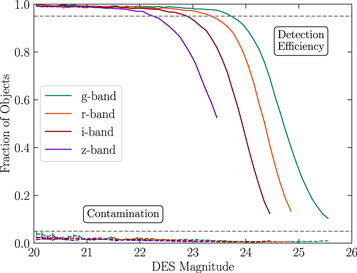
\includegraphics[width=3.12500in]{jira_imgs/404.png}

}

\subsubsection{LVV-T1074 - Sky Brightness precision}\label{lvv-t1074}

\begin{longtable}[]{llllll}
\toprule
Version & Status & Priority & Verification Type & Owner
\\\midrule
1 & Defined & Normal &
Analysis & Sam Schmidt
\\\bottomrule
\multicolumn{6}{c}{ Open \href{https://jira.lsstcorp.org/secure/Tests.jspa\#/testCase/LVV-T1074}{LVV-T1074} in Jira } \\
\end{longtable}

\paragraph{Verification Elements}\mbox{}\\

\begin{itemize}
\item \href{https://jira.lsstcorp.org/browse/LVV-277}{LVV-277} - LSR-REQ-0093-V-05: Photometric Performance5

\item \href{https://jira.lsstcorp.org/browse/LVV-13366}{LVV-13366} - OSS-REQ-0387-V-05: Sky Brightness precision

\end{itemize}

\paragraph{Test Items}\mbox{}\\









\paragraph{Test Procedure}\mbox{}\\
\begin{tabular}{p{4cm}p{12cm}}
\toprule
Step 1
& Description \\ \hline
\end{tabular}
{\scriptsize
Select a set of images at a variety of airmasses, Moon, and time to get
a range of sky brightness levels~

}
\begin{tabular}{p{3cm}p{13cm}}
\hline
            & Test Data \\ \hline
\end{tabular}
{\scriptsize
single visit images

}
\begin{tabular}{p{3cm}p{13cm}}
\hline
            & Expected Result \\ \hline
\end{tabular}

\begin{tabular}{p{4cm}p{12cm}}
\toprule
Step 2
& Description \\ \hline
\end{tabular}
{\scriptsize
Run DM Stack, part of which will generate polynomial fit to sky
brightness

}
\begin{tabular}{p{3cm}p{13cm}}
\hline
            & Test Data \\ \hline
\end{tabular}
{\scriptsize
images from step 1

}
\begin{tabular}{p{3cm}p{13cm}}
\hline
            & Expected Result \\ \hline
\end{tabular}
{\scriptsize
polynomial fit of sky brightness

}

\begin{tabular}{p{4cm}p{12cm}}
\toprule
Step 3
& Description \\ \hline
\end{tabular}
{\scriptsize
Compare sky brightness estimate from the polynomial fit to measures of
the sky brightness at specific points, test whether these agree to
SBPrec{[}1 percent{]}

}
\begin{tabular}{p{3cm}p{13cm}}
\hline
            & Test Data \\ \hline
\end{tabular}
{\scriptsize
polynomial fit from step 2

}
\begin{tabular}{p{3cm}p{13cm}}
\hline
            & Expected Result \\ \hline
\end{tabular}
{\scriptsize
pass fail for SBPrec test

}

\subsubsection{LVV-T1075 - Sky Brightness Precision 2 (Simulated Data)}\label{lvv-t1075}

\begin{longtable}[]{llllll}
\toprule
Version & Status & Priority & Verification Type & Owner
\\\midrule
1 & Defined & Normal &
Analysis & Sam Schmidt
\\\bottomrule
\multicolumn{6}{c}{ Open \href{https://jira.lsstcorp.org/secure/Tests.jspa\#/testCase/LVV-T1075}{LVV-T1075} in Jira } \\
\end{longtable}

\paragraph{Verification Elements}\mbox{}\\

\begin{itemize}
\item \href{https://jira.lsstcorp.org/browse/LVV-277}{LVV-277} - LSR-REQ-0093-V-05: Photometric Performance5

\item \href{https://jira.lsstcorp.org/browse/LVV-13366}{LVV-13366} - OSS-REQ-0387-V-05: Sky Brightness precision

\end{itemize}

\paragraph{Test Items}\mbox{}\\









\paragraph{Test Procedure}\mbox{}\\
\begin{tabular}{p{4cm}p{12cm}}
\toprule
Step 1
& Description \\ \hline
\end{tabular}
{\scriptsize
Generate simulated images with a known sky brightness, simulate
conditions with a range of airmass, Moon, atmosphere to get a range of
brightness conditions

}
\begin{tabular}{p{3cm}p{13cm}}
\hline
            & Test Data \\ \hline
\end{tabular}
{\scriptsize
New simulated image data

}
\begin{tabular}{p{3cm}p{13cm}}
\hline
            & Expected Result \\ \hline
\end{tabular}

\begin{tabular}{p{4cm}p{12cm}}
\toprule
Step 2
& Description \\ \hline
\end{tabular}
{\scriptsize
Run DM Stack processing, which generates polynomial fit to the sky
brightness

}
\begin{tabular}{p{3cm}p{13cm}}
\hline
            & Test Data \\ \hline
\end{tabular}
{\scriptsize
images from step 1

}
\begin{tabular}{p{3cm}p{13cm}}
\hline
            & Expected Result \\ \hline
\end{tabular}
{\scriptsize
sky brightness model

}

\begin{tabular}{p{4cm}p{12cm}}
\toprule
Step 3
& Description \\ \hline
\end{tabular}
{\scriptsize
Compare sky brightness to truth evaluated at points not used in the
polynomial grid determination, check that these agree to within SBPrec
{[}1 percent{]}

}
\begin{tabular}{p{3cm}p{13cm}}
\hline
            & Test Data \\ \hline
\end{tabular}
{\scriptsize
brightness model

}
\begin{tabular}{p{3cm}p{13cm}}
\hline
            & Expected Result \\ \hline
\end{tabular}
{\scriptsize
pass/fail for SBPrec test

}

\subsubsection{LVV-T1081 - Completeness vs. magnitude via external catalogs}\label{lvv-t1081}

\begin{longtable}[]{llllll}
\toprule
Version & Status & Priority & Verification Type & Owner
\\\midrule
1 & Defined & Normal &
Test & Jeffrey Carlin
\\\bottomrule
\multicolumn{6}{c}{ Open \href{https://jira.lsstcorp.org/secure/Tests.jspa\#/testCase/LVV-T1081}{LVV-T1081} in Jira } \\
\end{longtable}

\paragraph{Verification Elements}\mbox{}\\

\begin{itemize}
\item \href{https://jira.lsstcorp.org/browse/LVV-1315}{LVV-1315} - OSS-REQ-0164-V-01: Catalog Completeness and Reliability

\end{itemize}

\paragraph{Test Items}\mbox{}\\

Estimate completeness vs. magnitude for stars and galaxies by comparison
to an external ``truth'' catalog. Note that in practice there are no
external catalogs deep enough to separate stars from galaxies over the
relevant magnitude range, so that this comparison will likely measure
detection completeness of all sources from the external catalog.


\paragraph{Predecessors}\mbox{}\\
\href{https://jira.lsstcorp.org/secure/Tests.jspa\#/testCase/LVV-T1070}{LVV-T1070}
or
​\href{https://jira.lsstcorp.org/secure/Tests.jspa\#/testCase/LVV-T1071}{LVV-T1071}​​​






\paragraph{Test Procedure}\mbox{}\\
\begin{tabular}{p{4cm}p{12cm}}
\toprule
Step 1
& Description \\ \hline
\end{tabular}
{\scriptsize
Point the butler to appropriate overlapping data sets.

}
\begin{tabular}{p{3cm}p{13cm}}
\hline
            & Expected Result \\ \hline
\end{tabular}

\begin{tabular}{p{4cm}p{12cm}}
\toprule
Step 2
& Description \\ \hline
\end{tabular}
{\scriptsize
Point the butler to the appropriate deep LSST catalog.

}
\begin{tabular}{p{3cm}p{13cm}}
\hline
            & Expected Result \\ \hline
\end{tabular}

\begin{tabular}{p{4cm}p{12cm}}
\toprule
Step 3
& Description \\ \hline
\end{tabular}
{\scriptsize
For each object in the external reference catalog, check if there is a
corresponding detected object in the LSST catalog.\\[2\baselineskip]The
matching should be done via position, but may be improved by requiring
similar magnitudes between the two catalogs (keeping in mind that
variable, yet persistent, objects may present different brightness, and
thus would not necessarily pass a magnitude criterion).

}
\begin{tabular}{p{3cm}p{13cm}}
\hline
            & Expected Result \\ \hline
\end{tabular}

\begin{tabular}{p{4cm}p{12cm}}
\toprule
Step 4
& Description \\ \hline
\end{tabular}
{\scriptsize
In magnitude bins, count the fraction of objects from the external
catalog that had a corresponding object in the LSST dataset. Plot this
fraction (the ``completeness'') as a function of magnitude.

}
\begin{tabular}{p{3cm}p{13cm}}
\hline
            & Expected Result \\ \hline
\end{tabular}
{\scriptsize
A figure similar to Fig. 15 of the
\href{https://arxiv.org/pdf/1702.08449.pdf}{HSC DR1 paper}.

}

\subsubsection{LVV-T1082 - Completeness vs. magnitude via injected sources}\label{lvv-t1082}

\begin{longtable}[]{llllll}
\toprule
Version & Status & Priority & Verification Type & Owner
\\\midrule
1 & Defined & Normal &
Test & Jeffrey Carlin
\\\bottomrule
\multicolumn{6}{c}{ Open \href{https://jira.lsstcorp.org/secure/Tests.jspa\#/testCase/LVV-T1082}{LVV-T1082} in Jira } \\
\end{longtable}

\paragraph{Verification Elements}\mbox{}\\

\begin{itemize}
\item \href{https://jira.lsstcorp.org/browse/LVV-1315}{LVV-1315} - OSS-REQ-0164-V-01: Catalog Completeness and Reliability

\end{itemize}

\paragraph{Test Items}\mbox{}\\

Estimate completeness vs. magnitude for stars and galaxies by inserting
artificial sources into observed LSST data.


\paragraph{Predecessors}\mbox{}\\
\href{https://jira.lsstcorp.org/secure/Tests.jspa\#/testCase/LVV-T1070}{LVV-T1070}
or
​\href{https://jira.lsstcorp.org/secure/Tests.jspa\#/testCase/LVV-T1071}{LVV-T1071}​​​






\paragraph{Test Procedure}\mbox{}\\
\begin{tabular}{p{4cm}p{12cm}}
\toprule
Step 1
& Description \\ \hline
\end{tabular}
{\scriptsize
Identify several tracts in the observed data, spanning a range of
Galactic latitudes/source densities.~

}
\begin{tabular}{p{3cm}p{13cm}}
\hline
            & Expected Result \\ \hline
\end{tabular}

\begin{tabular}{p{4cm}p{12cm}}
\toprule
Step 2
& Description \\ \hline
\end{tabular}
{\scriptsize
Create catalogs of artificial sources to be inserted into the images. To
ensure statistically robust results, at least 1000 objects per magnitude
bin should be included.

}
\begin{tabular}{p{3cm}p{13cm}}
\hline
            & Test Data \\ \hline
\end{tabular}
{\scriptsize
The artificial star catalog should span the range of colors typical of
Milky Way stars, and the expected magnitudes to which the input data are
sensitive (e.g., the GalFast simulated catalog). Artificial galaxies
should be drawn from a synthetic catalog (e.g., the DESC Data Challenge
galaxy catalogs).

}
\begin{tabular}{p{3cm}p{13cm}}
\hline
            & Expected Result \\ \hline
\end{tabular}

\begin{tabular}{p{4cm}p{12cm}}
\toprule
Step 3
& Description \\ \hline
\end{tabular}
{\scriptsize
Identify the images into which you will insert sources, and run the fake
source code (in the current LSST Stack, the `Synpipe' routine(s)).
Ideally these should be injected into the individual visit images, but
if that is computationally prohibitive, inserting them into coadds would
be acceptable.

}
\begin{tabular}{p{3cm}p{13cm}}
\hline
            & Expected Result \\ \hline
\end{tabular}

\begin{tabular}{p{4cm}p{12cm}}
\toprule
Step 4
& Description \\ \hline
\end{tabular}
{\scriptsize
Run the source detection and measurement algorithms on the images
resulting from the previous steps.

}
\begin{tabular}{p{3cm}p{13cm}}
\hline
            & Expected Result \\ \hline
\end{tabular}

\begin{tabular}{p{4cm}p{12cm}}
\toprule
Step 5
& Description \\ \hline
\end{tabular}
{\scriptsize
Point the Butler to the catalog resulting from the previous step.

}
\begin{tabular}{p{3cm}p{13cm}}
\hline
            & Expected Result \\ \hline
\end{tabular}

\begin{tabular}{p{4cm}p{12cm}}
\toprule
Step 6
& Description \\ \hline
\end{tabular}
{\scriptsize
Define the criteria for matching of sources. Because the positions of
injected sources are known, a small matching radius can be used.

}
\begin{tabular}{p{3cm}p{13cm}}
\hline
            & Expected Result \\ \hline
\end{tabular}

\begin{tabular}{p{4cm}p{12cm}}
\toprule
Step 7
& Description \\ \hline
\end{tabular}
{\scriptsize
For each object in the input artificial source catalog, check if there
is a corresponding detected object in the output LSST
catalog.\\[2\baselineskip]The matching should be done via position, but
may be improved by requiring similar magnitudes between the two
catalogs.

}
\begin{tabular}{p{3cm}p{13cm}}
\hline
            & Expected Result \\ \hline
\end{tabular}

\begin{tabular}{p{4cm}p{12cm}}
\toprule
Step 8
& Description \\ \hline
\end{tabular}
{\scriptsize
In magnitude bins, count the fraction of objects from the input
``truth'' catalog that had a corresponding detected object in the LSST
dataset. Plot this fraction (the ``completeness'') as a function of
magnitude, for (1) all sources, (2) objects inserted as stars, and (3)
objects inserted as galaxies.

}
\begin{tabular}{p{3cm}p{13cm}}
\hline
            & Expected Result \\ \hline
\end{tabular}
{\scriptsize
A figure similar to Fig. 15 of the
\href{https://arxiv.org/pdf/1702.08449.pdf}{HSC DR1 paper}, but with
separate curves for stars and galaxies.

}

\subsubsection{LVV-T1083 - Single Visit Ellipticity Residuals w/ on sky data}\label{lvv-t1083}

\begin{longtable}[]{llllll}
\toprule
Version & Status & Priority & Verification Type & Owner
\\\midrule
1 & Defined & Normal &
Analysis & Imram Hasan
\\\bottomrule
\multicolumn{6}{c}{ Open \href{https://jira.lsstcorp.org/secure/Tests.jspa\#/testCase/LVV-T1083}{LVV-T1083} in Jira } \\
\end{longtable}

\paragraph{Verification Elements}\mbox{}\\

\begin{itemize}
\item \href{https://jira.lsstcorp.org/browse/LVV-1366}{LVV-1366} - OSS-REQ-0390-V-01: Ellipticity Correlations

\end{itemize}

\paragraph{Test Items}\mbox{}\\

Confirm the amplitude of elipticity residual correlations is within spec


\paragraph{Predecessors}\mbox{}\\
\href{https://jira.lsstcorp.org/secure/Tests.jspa\#/testCase/LVV-T1070}{LVV-T1070}
or
​\href{https://jira.lsstcorp.org/secure/Tests.jspa\#/testCase/LVV-T1071}{LVV-T1071}​​​






\paragraph{Test Procedure}\mbox{}\\
\begin{tabular}{p{4cm}p{12cm}}
\toprule
Step 1
& Description \\ \hline
\end{tabular}
{\scriptsize
Point the butler at the single visit comissioning data. We will need the
individual PSF models and the calexp catalogs

}
\begin{tabular}{p{3cm}p{13cm}}
\hline
            & Expected Result \\ \hline
\end{tabular}

\begin{tabular}{p{4cm}p{12cm}}
\toprule
Step 2
& Description \\ \hline
\end{tabular}
{\scriptsize
Obtain calexps src catalogs that are well representative of observing
conditions, eg cover a range of airmasses, seeing conditions, moon
brightness etc.\\[2\baselineskip]obtain the PSF models from these
calexps as well.

}
\begin{tabular}{p{3cm}p{13cm}}
\hline
            & Expected Result \\ \hline
\end{tabular}

\begin{tabular}{p{4cm}p{12cm}}
\toprule
Step 3
& Description \\ \hline
\end{tabular}
{\scriptsize
Consider separately stars that were included in PSF modeling and stars
that were not included in PSF modeling. The fiduciual result for this
test should use the stars that were not included in PSF modeling. The
stars that were included in PSF modeling will still be useful for
diagnostic purposes.

}
\begin{tabular}{p{3cm}p{13cm}}
\hline
            & Expected Result \\ \hline
\end{tabular}

\begin{tabular}{p{4cm}p{12cm}}
\toprule
Step 4
& Description \\ \hline
\end{tabular}
{\scriptsize
For each stellar sample, compute all Rowe statistics over angular scales
ranging from less than 1 arcmin to greater than 5
arcmin.\\[2\baselineskip]This will require the PSF model for calculating
residuals. To calculate residuals, obtain the PSF model evaluated at the
positions of stars of interest, and find the difference in the measured
ellipticity of stars, and the model ellipticity.

}
\begin{tabular}{p{3cm}p{13cm}}
\hline
            & Expected Result \\ \hline
\end{tabular}

\begin{tabular}{p{4cm}p{12cm}}
\toprule
Step 5
& Description \\ \hline
\end{tabular}
{\scriptsize
Extract the amplitudes of the Rowe statistics at angular scales of 1
arcmin and less, and 5 arcmin and larger

}
\begin{tabular}{p{3cm}p{13cm}}
\hline
            & Expected Result \\ \hline
\end{tabular}

\begin{tabular}{p{4cm}p{12cm}}
\toprule
Step 6
& Description \\ \hline
\end{tabular}
{\scriptsize
For each angular scale (\textless{}1 arcmin and \textgreater{}5 arcmin),
for each Rowe statistic, collect the amplitudes of the Rho statistics.

}
\begin{tabular}{p{3cm}p{13cm}}
\hline
            & Expected Result \\ \hline
\end{tabular}

\begin{tabular}{p{4cm}p{12cm}}
\toprule
Step 7
& Description \\ \hline
\end{tabular}
{\scriptsize
Calculate the medians from the amplitudes corresponding to each angular
scale, for each Rowe statistic.

}
\begin{tabular}{p{3cm}p{13cm}}
\hline
            & Expected Result \\ \hline
\end{tabular}

\begin{tabular}{p{4cm}p{12cm}}
\toprule
Step 8
& Description \\ \hline
\end{tabular}
{\scriptsize
Calculate the fraction of exposures where the medians of amplitudes are
within the specifications for individual calexp exposures, and outside
of specifications for the \textless{}1 arcsec and \textgreater{}5 arcsec
scales

}
\begin{tabular}{p{3cm}p{13cm}}
\hline
            & Expected Result \\ \hline
\end{tabular}

\begin{tabular}{p{4cm}p{12cm}}
\toprule
Step 9
& Description \\ \hline
\end{tabular}
{\scriptsize
Confirm that the fraction of single visit Rowe Statistics outside of
spec is less than 15\% (TEF)

}
\begin{tabular}{p{3cm}p{13cm}}
\hline
            & Expected Result \\ \hline
\end{tabular}

\subsubsection{LVV-T1084 - Smoothness of Rowe statistics on angular scales of 1 arcmin \textless{}
theta \textless{} 5 arcmin}\label{lvv-t1084}

\begin{longtable}[]{llllll}
\toprule
Version & Status & Priority & Verification Type & Owner
\\\midrule
1 & Defined & Normal &
Analysis & Imram Hasan
\\\bottomrule
\multicolumn{6}{c}{ Open \href{https://jira.lsstcorp.org/secure/Tests.jspa\#/testCase/LVV-T1084}{LVV-T1084} in Jira } \\
\end{longtable}

\paragraph{Verification Elements}\mbox{}\\

\begin{itemize}
\item \href{https://jira.lsstcorp.org/browse/LVV-1366}{LVV-1366} - OSS-REQ-0390-V-01: Ellipticity Correlations

\end{itemize}

\paragraph{Test Items}\mbox{}\\



\paragraph{Predecessors}\mbox{}\\
\href{https://jira.lsstcorp.org/secure/Tests.jspa\#/testCase/LVV-T361}{LVV-T361
(1.0)}






\paragraph{Test Procedure}\mbox{}\\
\begin{tabular}{p{4cm}p{12cm}}
\toprule
Step 1
& Description \\ \hline
\end{tabular}
{\scriptsize
Get the final Rowe statistics that were calculated in test case
\href{https://jira.lsstcorp.org/secure/Tests.jspa\#/testCase/LVV-T361}{LVV-T361
(1.0)}in step 4

}
\begin{tabular}{p{3cm}p{13cm}}
\hline
            & Expected Result \\ \hline
\end{tabular}

\begin{tabular}{p{4cm}p{12cm}}
\toprule
Step 2
& Description \\ \hline
\end{tabular}
{\scriptsize
For all Rowe statistics, examine by eye the amplitudes between the
angular scales of 1 arcmin \textless{} theta \textless{} 5 arcmin

}
\begin{tabular}{p{3cm}p{13cm}}
\hline
            & Expected Result \\ \hline
\end{tabular}

\begin{tabular}{p{4cm}p{12cm}}
\toprule
Step 3
& Description \\ \hline
\end{tabular}
{\scriptsize
Confirm that the amplitudes vary smoothly between these angular scales

}
\begin{tabular}{p{3cm}p{13cm}}
\hline
            & Expected Result \\ \hline
\end{tabular}

\subsubsection{LVV-T1278 - Relative Astrometric Performance (Repeatability)}\label{lvv-t1278}

\begin{longtable}[]{llllll}
\toprule
Version & Status & Priority & Verification Type & Owner
\\\midrule
1 & Defined & Normal &
Test & Bryce Kalmbach
\\\bottomrule
\multicolumn{6}{c}{ Open \href{https://jira.lsstcorp.org/secure/Tests.jspa\#/testCase/LVV-T1278}{LVV-T1278} in Jira } \\
\end{longtable}

\paragraph{Verification Elements}\mbox{}\\

\begin{itemize}
\item \href{https://jira.lsstcorp.org/browse/LVV-1363}{LVV-1363} - OSS-REQ-0388-V-01: Astrometric Performance

\end{itemize}

\paragraph{Test Items}\mbox{}\\

Verify that relative astrometric separations are as accurate as
specified








\paragraph{Test Procedure}\mbox{}\\
\begin{tabular}{p{4cm}p{12cm}}
\toprule
Step 1
& Description \\ \hline
\end{tabular}
{\scriptsize
Image an average field. Repeat at different airmasses.

}
\begin{tabular}{p{3cm}p{13cm}}
\hline
            & Expected Result \\ \hline
\end{tabular}

\begin{tabular}{p{4cm}p{12cm}}
\toprule
Step 2
& Description \\ \hline
\end{tabular}
{\scriptsize
Run source detection and astrometric measurement on images from step 1

}
\begin{tabular}{p{3cm}p{13cm}}
\hline
            & Test Data \\ \hline
\end{tabular}
{\scriptsize
Images from Step 1

}
\begin{tabular}{p{3cm}p{13cm}}
\hline
            & Expected Result \\ \hline
\end{tabular}

\begin{tabular}{p{4cm}p{12cm}}
\toprule
Step 3
& Description \\ \hline
\end{tabular}
{\scriptsize
Calculate the separations between all sources detected in step 2

}
\begin{tabular}{p{3cm}p{13cm}}
\hline
            & Test Data \\ \hline
\end{tabular}
{\scriptsize
Matched source catalogs from Step 2

}
\begin{tabular}{p{3cm}p{13cm}}
\hline
            & Expected Result \\ \hline
\end{tabular}

\begin{tabular}{p{4cm}p{12cm}}
\toprule
Step 4
& Description \\ \hline
\end{tabular}
{\scriptsize
Compare source separations from step 3. Calculate RMS for each pair
across set of visits.

}
\begin{tabular}{p{3cm}p{13cm}}
\hline
            & Test Data \\ \hline
\end{tabular}
{\scriptsize
Source separations from Step 3.

}
\begin{tabular}{p{3cm}p{13cm}}
\hline
            & Expected Result \\ \hline
\end{tabular}

\begin{tabular}{p{4cm}p{12cm}}
\toprule
Step 5
& Description \\ \hline
\end{tabular}
{\scriptsize
Examine distribution of source separation RMS from step 4 for all pairs
of sources separated by \textasciitilde{} 5 arcminutes. Verify that the
median in these measurements is \textless{}= 10 milliarcseconds

}
\begin{tabular}{p{3cm}p{13cm}}
\hline
            & Test Data \\ \hline
\end{tabular}
{\scriptsize
Source separations form Step 4. Positions from Matched Source catalogs
from Step 2.

}
\begin{tabular}{p{3cm}p{13cm}}
\hline
            & Expected Result \\ \hline
\end{tabular}

\begin{tabular}{p{4cm}p{12cm}}
\toprule
Step 6
& Description \\ \hline
\end{tabular}
{\scriptsize
Verify that no more than 10\% of the source pairs separated by
\textasciitilde{} 5 arcminutes have separation RMS greater than 20
milliarcseconds

}
\begin{tabular}{p{3cm}p{13cm}}
\hline
            & Test Data \\ \hline
\end{tabular}
{\scriptsize
Source separations form Step 4. Positions from Matched Source catalogs
from Step 2.

}
\begin{tabular}{p{3cm}p{13cm}}
\hline
            & Expected Result \\ \hline
\end{tabular}

\begin{tabular}{p{4cm}p{12cm}}
\toprule
Step 7
& Description \\ \hline
\end{tabular}
{\scriptsize
Examine distribution of source separation RMS from step 4 for all pairs
of sources separated by \textasciitilde{} 20 arcminutes. Verify that the
median in these measurements is \textless{}= 10 milliarcseconds

}
\begin{tabular}{p{3cm}p{13cm}}
\hline
            & Test Data \\ \hline
\end{tabular}
{\scriptsize
Source separations form Step 4. Positions from Matched Source catalogs
from Step 2.

}
\begin{tabular}{p{3cm}p{13cm}}
\hline
            & Expected Result \\ \hline
\end{tabular}

\begin{tabular}{p{4cm}p{12cm}}
\toprule
Step 8
& Description \\ \hline
\end{tabular}
{\scriptsize
Verify that no more than 10\% of the source pairs separated by
\textasciitilde{} 20 arcminutes have separation RMS greater than 20
milliarcseconds

}
\begin{tabular}{p{3cm}p{13cm}}
\hline
            & Test Data \\ \hline
\end{tabular}
{\scriptsize
Source separations form Step 4. Positions from Matched Source catalogs
from Step 2.

}
\begin{tabular}{p{3cm}p{13cm}}
\hline
            & Expected Result \\ \hline
\end{tabular}

\begin{tabular}{p{4cm}p{12cm}}
\toprule
Step 9
& Description \\ \hline
\end{tabular}
{\scriptsize
Examine distribution of source separation RMS from step 4 for all pairs
of sources separated by \textasciitilde{} 200 arcminutes. Verify that
the median in these measurements is \textless{}= 15 milliarcseconds

}
\begin{tabular}{p{3cm}p{13cm}}
\hline
            & Test Data \\ \hline
\end{tabular}
{\scriptsize
Source separations form Step 4. Positions from Matched Source catalogs
from Step 2.

}
\begin{tabular}{p{3cm}p{13cm}}
\hline
            & Expected Result \\ \hline
\end{tabular}

\begin{tabular}{p{4cm}p{12cm}}
\toprule
Step 10
& Description \\ \hline
\end{tabular}
{\scriptsize
Verify that no more than 10\% of the source pairs separated by
\textasciitilde{} 200 arcminutes have separation RMS greater than 30
milliarcseconds

}
\begin{tabular}{p{3cm}p{13cm}}
\hline
            & Test Data \\ \hline
\end{tabular}
{\scriptsize
Source separations form Step 4. Positions from Matched Source catalogs
from Step 2.

}
\begin{tabular}{p{3cm}p{13cm}}
\hline
            & Expected Result \\ \hline
\end{tabular}

\subsection{ Draft Test Cases}

\subsubsection{LVV-T293 - On-sky Observations: Single-visit Key Performance Metrics}\label{lvv-t293}

\begin{longtable}[]{llllll}
\toprule
Version & Status & Priority & Verification Type & Owner
\\\midrule
1 & Draft & Normal &
Demonstration & Keith Bechtol
\\\bottomrule
\multicolumn{6}{c}{ Open \href{https://jira.lsstcorp.org/secure/Tests.jspa\#/testCase/LVV-T293}{LVV-T293} in Jira } \\
\end{longtable}

\paragraph{Verification Elements}\mbox{}\\

\begin{itemize}
\item \href{https://jira.lsstcorp.org/browse/LVV-1544}{LVV-1544} - OSS-REQ-0228-V-02: Image Size in Pixels

\end{itemize}

\paragraph{Test Items}\mbox{}\\

Perform repeated observations of a set of 20 to 30 fields to evaluate
single-visit science performance metrics such as system throughput,
image quality, and astrometric and photometric repeatability. The fields
should be selected to span a range of object densities (e.g., by
sampling different Galactic latitudes) and should be observed under a
range of environmental conditions, including a range of airmass and sky
brightness. (WHAT RANGE?) The target fields should include
spectrophotometric standards such as DA white dwarfs to be used to
evaluate the absolute photometric calibration (HOW
MANY?)\\[2\baselineskip]The ~pointings in each field will be dithered to
allow tests of delivered image quality, throughput, calibration, and
astrometry across the full field of view. Photometric conditions are
required.\\[2\baselineskip]Sub-percent Photometry: Faint DA White Dwarf
Spectrophotometric Standards for Astrophysical Observatories\\
\url{https://arxiv.org/abs/1811.12534}\\[2\baselineskip]\textbf{Example
observations:}\\
20 fields x 5 visits x 6 filters x 5 epochs = 20 fields x 25 visits x 6
filters.








\paragraph{Test Procedure}\mbox{}\\
\begin{tabular}{p{4cm}p{12cm}}
\toprule
Step 1
& Description \\ \hline
\end{tabular}
{\scriptsize

}
\begin{tabular}{p{3cm}p{13cm}}
\hline
            & Expected Result \\ \hline
\end{tabular}

\subsubsection{LVV-T294 - On-sky Observations: Full-survey Key Performance Metrics}\label{lvv-t294}

\begin{longtable}[]{llllll}
\toprule
Version & Status & Priority & Verification Type & Owner
\\\midrule
1 & Draft & Normal &
Demonstration & Keith Bechtol
\\\bottomrule
\multicolumn{6}{c}{ Open \href{https://jira.lsstcorp.org/secure/Tests.jspa\#/testCase/LVV-T294}{LVV-T294} in Jira } \\
\end{longtable}

\paragraph{Verification Elements}\mbox{}\\

\begin{itemize}
\item \href{https://jira.lsstcorp.org/browse/LVV-1545}{LVV-1545} - OSS-REQ-0228-V-03: Image Quality vs Field

\item \href{https://jira.lsstcorp.org/browse/LVV-7213}{LVV-7213} - OSS-REQ-0228-V-04: Image Quality in Encircled Energy

\item \href{https://jira.lsstcorp.org/browse/LVV-7214}{LVV-7214} - OSS-REQ-0228-V-05: System Contribution to Image Quality

\end{itemize}

\paragraph{Test Items}\mbox{}\\

Repeated observations of a smaller number of fields reaching cumulative
exposures equivalent to the 10-year stack in the wide-fast-deep survey,
specifically, 200 visits in both the r and i band. These ~observations
are designed to measure residual PSF ellipticities, ~and to test
transient, variable, and moving object detection over a range of
timescales. Three fields should be chosen along the ecliptic that
together span a range of source densities. Each field should be observed
in multiple epochsdistributed over at least 3 consecutive nights and
cover a range of airmasses. Dithered pointings will be used to
approximate the coverage pattern expected in the wide-fast-deep
survey.\\[2\baselineskip]Estimated ~observing time = 34 seconds * 200
visits * 2 filters * 3 (dither pattern) * 3 fields =
\textasciitilde{}36hrs.








\paragraph{Test Procedure}\mbox{}\\
\begin{tabular}{p{4cm}p{12cm}}
\toprule
Step 1
& Description \\ \hline
\end{tabular}
{\scriptsize

}
\begin{tabular}{p{3cm}p{13cm}}
\hline
            & Expected Result \\ \hline
\end{tabular}

\subsubsection{LVV-T295 - Data Processing Campaign: Single-visit Key Performance Metrics}\label{lvv-t295}

\begin{longtable}[]{llllll}
\toprule
Version & Status & Priority & Verification Type & Owner
\\\midrule
1 & Draft & Normal &
Demonstration & Keith Bechtol
\\\bottomrule
\multicolumn{6}{c}{ Open \href{https://jira.lsstcorp.org/secure/Tests.jspa\#/testCase/LVV-T295}{LVV-T295} in Jira } \\
\end{longtable}

\paragraph{Verification Elements}\mbox{}\\

\begin{itemize}
\item \href{https://jira.lsstcorp.org/browse/LVV-1544}{LVV-1544} - OSS-REQ-0228-V-02: Image Size in Pixels

\end{itemize}

\paragraph{Test Items}\mbox{}\\









\paragraph{Test Procedure}\mbox{}\\
\begin{tabular}{p{4cm}p{12cm}}
\toprule
Step 1
& Description \\ \hline
\end{tabular}
{\scriptsize

}
\begin{tabular}{p{3cm}p{13cm}}
\hline
            & Expected Result \\ \hline
\end{tabular}

\subsubsection{LVV-T296 - Data Processing Campaign: Full-survey Key Performance Metrics}\label{lvv-t296}

\begin{longtable}[]{llllll}
\toprule
Version & Status & Priority & Verification Type & Owner
\\\midrule
1 & Draft & Normal &
Demonstration & Keith Bechtol
\\\bottomrule
\multicolumn{6}{c}{ Open \href{https://jira.lsstcorp.org/secure/Tests.jspa\#/testCase/LVV-T296}{LVV-T296} in Jira } \\
\end{longtable}

\paragraph{Verification Elements}\mbox{}\\

\begin{itemize}
\item \href{https://jira.lsstcorp.org/browse/LVV-1545}{LVV-1545} - OSS-REQ-0228-V-03: Image Quality vs Field

\item \href{https://jira.lsstcorp.org/browse/LVV-7213}{LVV-7213} - OSS-REQ-0228-V-04: Image Quality in Encircled Energy

\item \href{https://jira.lsstcorp.org/browse/LVV-7214}{LVV-7214} - OSS-REQ-0228-V-05: System Contribution to Image Quality

\end{itemize}

\paragraph{Test Items}\mbox{}\\









\paragraph{Test Procedure}\mbox{}\\
\begin{tabular}{p{4cm}p{12cm}}
\toprule
Step 1
& Description \\ \hline
\end{tabular}
{\scriptsize

}
\begin{tabular}{p{3cm}p{13cm}}
\hline
            & Expected Result \\ \hline
\end{tabular}

\subsubsection{LVV-T298 - Cross-band Astrometric Performance}\label{lvv-t298}

\begin{longtable}[]{llllll}
\toprule
Version & Status & Priority & Verification Type & Owner
\\\midrule
1 & Draft & Normal &
Test & Keith Bechtol
\\\bottomrule
\multicolumn{6}{c}{ Open \href{https://jira.lsstcorp.org/secure/Tests.jspa\#/testCase/LVV-T298}{LVV-T298} in Jira } \\
\end{longtable}

\paragraph{Verification Elements}\mbox{}\\

\begin{itemize}
\item \href{https://jira.lsstcorp.org/browse/LVV-1544}{LVV-1544} - OSS-REQ-0228-V-02: Image Size in Pixels

\end{itemize}

\paragraph{Test Items}\mbox{}\\









\paragraph{Test Procedure}\mbox{}\\
\begin{tabular}{p{4cm}p{12cm}}
\toprule
Step 1
& Description \\ \hline
\end{tabular}
{\scriptsize

}
\begin{tabular}{p{3cm}p{13cm}}
\hline
            & Expected Result \\ \hline
\end{tabular}

\subsubsection{LVV-T299 - Relative Astrometric Performance}\label{lvv-t299}

\begin{longtable}[]{llllll}
\toprule
Version & Status & Priority & Verification Type & Owner
\\\midrule
1 & Draft & Normal &
Test & Keith Bechtol
\\\bottomrule
\multicolumn{6}{c}{ Open \href{https://jira.lsstcorp.org/secure/Tests.jspa\#/testCase/LVV-T299}{LVV-T299} in Jira } \\
\end{longtable}

\paragraph{Verification Elements}\mbox{}\\

\begin{itemize}
\item \href{https://jira.lsstcorp.org/browse/LVV-1544}{LVV-1544} - OSS-REQ-0228-V-02: Image Size in Pixels

\end{itemize}

\paragraph{Test Items}\mbox{}\\









\paragraph{Test Procedure}\mbox{}\\
\begin{tabular}{p{4cm}p{12cm}}
\toprule
Step 1
& Description \\ \hline
\end{tabular}
{\scriptsize

}
\begin{tabular}{p{3cm}p{13cm}}
\hline
            & Expected Result \\ \hline
\end{tabular}

\subsubsection{LVV-T360 - Off Zenith Image Quality Degradation}\label{lvv-t360}

\begin{longtable}[]{llllll}
\toprule
Version & Status & Priority & Verification Type & Owner
\\\midrule
1 & Draft & Normal &
Analysis & Keith Bechtol
\\\bottomrule
\multicolumn{6}{c}{ Open \href{https://jira.lsstcorp.org/secure/Tests.jspa\#/testCase/LVV-T360}{LVV-T360} in Jira } \\
\end{longtable}

\paragraph{Verification Elements}\mbox{}\\

\begin{itemize}
\item \href{https://jira.lsstcorp.org/browse/LVV-1543}{LVV-1543} - OSS-REQ-0228-V-01: Image Quality Off-Zenith Degredation

\end{itemize}

\paragraph{Test Items}\mbox{}\\









\paragraph{Test Procedure}\mbox{}\\
\begin{tabular}{p{4cm}p{12cm}}
\toprule
Step 1
& Description \\ \hline
\end{tabular}
{\scriptsize

}
\begin{tabular}{p{3cm}p{13cm}}
\hline
            & Expected Result \\ \hline
\end{tabular}

\subsubsection{LVV-T442 - Control Ghosts in Coadds}\label{lvv-t442}

\begin{longtable}[]{llllll}
\toprule
Version & Status & Priority & Verification Type & Owner
\\\midrule
1 & Draft & Normal &
Analysis & Keith Bechtol
\\\bottomrule
\multicolumn{6}{c}{ Open \href{https://jira.lsstcorp.org/secure/Tests.jspa\#/testCase/LVV-T442}{LVV-T442} in Jira } \\
\end{longtable}

\paragraph{Verification Elements}\mbox{}\\

None.

\paragraph{Test Items}\mbox{}\\









\paragraph{Test Procedure}\mbox{}\\
\begin{tabular}{p{4cm}p{12cm}}
\toprule
Step 1
& Description \\ \hline
\end{tabular}
{\scriptsize

}
\begin{tabular}{p{3cm}p{13cm}}
\hline
            & Expected Result \\ \hline
\end{tabular}

\subsubsection{LVV-T461 - Filter Out of Band Constraints}\label{lvv-t461}

\begin{longtable}[]{llllll}
\toprule
Version & Status & Priority & Verification Type & Owner
\\\midrule
1 & Draft & Normal &
Analysis & Robert Morgan
\\\bottomrule
\multicolumn{6}{c}{ Open \href{https://jira.lsstcorp.org/secure/Tests.jspa\#/testCase/LVV-T461}{LVV-T461} in Jira } \\
\end{longtable}

\paragraph{Verification Elements}\mbox{}\\

None.

\paragraph{Test Items}\mbox{}\\

Verify that the out-of-band filter transmission (leakage) is low enough
to pass OSS-237








\paragraph{Test Procedure}\mbox{}\\
\begin{tabular}{p{4cm}p{12cm}}
\toprule
Step 1
& Description \\ \hline
\end{tabular}
{\scriptsize
Data Collection

}
\begin{tabular}{p{3cm}p{13cm}}
\hline
            & Test Data \\ \hline
\end{tabular}
{\scriptsize
Using the collimated beam projector, each amplifier on the focal plane
is to be targeted with wavelengths 300 nm to 1200 nm. After ISR is
applied, the incident light and the transmitted light are to be compared
such that filter transmission as a function of wavelength is known. This
process is to be repeated for each filter.

}
\begin{tabular}{p{3cm}p{13cm}}
\hline
            & Expected Result \\ \hline
\end{tabular}

\begin{tabular}{p{4cm}p{12cm}}
\toprule
Step 2
& Description \\ \hline
\end{tabular}
{\scriptsize
For each filter and amplifier, read in the transmission curve.

}
\begin{tabular}{p{3cm}p{13cm}}
\hline
            & Test Data \\ \hline
\end{tabular}
{\scriptsize
Transmission curve for each filter and amplifier.

}
\begin{tabular}{p{3cm}p{13cm}}
\hline
            & Expected Result \\ \hline
\end{tabular}

\begin{tabular}{p{4cm}p{12cm}}
\toprule
Step 3
& Description \\ \hline
\end{tabular}
{\scriptsize
Calculate the central wavelength and FWHM of the transmission curve.
Select the region of the curve between 300 nm and 1200 nm, but outside
one FWHM from the central wavelength.

}
\begin{tabular}{p{3cm}p{13cm}}
\hline
            & Test Data \\ \hline
\end{tabular}
{\scriptsize
Transmission curve for each filter and amplifier.

}
\begin{tabular}{p{3cm}p{13cm}}
\hline
            & Expected Result \\ \hline
\end{tabular}

\begin{tabular}{p{4cm}p{12cm}}
\toprule
Step 4
& Description \\ \hline
\end{tabular}
{\scriptsize
Bin the transmission curve values in 10 nm segments.

}
\begin{tabular}{p{3cm}p{13cm}}
\hline
            & Test Data \\ \hline
\end{tabular}
{\scriptsize
Out-of-band transmission curve for each filter and amplifier.

}
\begin{tabular}{p{3cm}p{13cm}}
\hline
            & Expected Result \\ \hline
\end{tabular}

\begin{tabular}{p{4cm}p{12cm}}
\toprule
Step 5
& Description \\ \hline
\end{tabular}
{\scriptsize
Iterate through the segments and obtain the following quantities:

\begin{enumerate}
\tightlist
\item
  The average transmission in each segment
\item
  The maximum transmission in each segment
\item
  The peak transmission of all segments
\item
  The number of segments with maximum transmission larger than 0.01
  percent
\item
  The cumulative integrated transmission

  \begin{enumerate}
  \tightlist
  \item
    Above wavelengths of 1050 nm, multiply the filter response by the
    silicon response when performing the integration.
  \end{enumerate}
\end{enumerate}

}
\begin{tabular}{p{3cm}p{13cm}}
\hline
            & Test Data \\ \hline
\end{tabular}
{\scriptsize
Binned out-of-band transmission curve for each filter and amplifier.

}
\begin{tabular}{p{3cm}p{13cm}}
\hline
            & Expected Result \\ \hline
\end{tabular}

\begin{tabular}{p{4cm}p{12cm}}
\toprule
Step 6
& Description \\ \hline
\end{tabular}
{\scriptsize
Calculate the percent of segments with maximum transmission larger than
0.01 percent

}
\begin{tabular}{p{3cm}p{13cm}}
\hline
            & Test Data \\ \hline
\end{tabular}
{\scriptsize
Number of segments with maximum transmission larger than 0.01 percent
obtained from the iteration.

}
\begin{tabular}{p{3cm}p{13cm}}
\hline
            & Expected Result \\ \hline
\end{tabular}

\begin{tabular}{p{4cm}p{12cm}}
\toprule
Step 7
& Description \\ \hline
\end{tabular}
{\scriptsize
Iterate through the segments a second time to get the cumulative
integrated transmission after the wavelength where the transmission
falls below 0.1 percent of the peak transmission of all the segments
found from the previous iteration.

}
\begin{tabular}{p{3cm}p{13cm}}
\hline
            & Test Data \\ \hline
\end{tabular}
{\scriptsize
Binned out-of-band transmission curve for each filter and amplifier.

}
\begin{tabular}{p{3cm}p{13cm}}
\hline
            & Expected Result \\ \hline
\end{tabular}

\begin{tabular}{p{4cm}p{12cm}}
\toprule
Step 8
& Description \\ \hline
\end{tabular}
{\scriptsize
Calculate the ratio of the cumulative integrated transmission after the
wavelength where the transmission falls below 0.1 percent of the peak
transmission of all the segments to the total integrated transmission of
all segments.

}
\begin{tabular}{p{3cm}p{13cm}}
\hline
            & Test Data \\ \hline
\end{tabular}
{\scriptsize
Integrated transmission after 0.1 percent of peak obtained from second
iteration and total integrated transmission obtained from first
iteration.

}
\begin{tabular}{p{3cm}p{13cm}}
\hline
            & Expected Result \\ \hline
\end{tabular}

\begin{tabular}{p{4cm}p{12cm}}
\toprule
Step 9
& Description \\ \hline
\end{tabular}
{\scriptsize
Check that all of the average transmissions are below 0.01 percent.

}
\begin{tabular}{p{3cm}p{13cm}}
\hline
            & Test Data \\ \hline
\end{tabular}
{\scriptsize
Average transmission in each 10 nm segment found during first iteration.

}
\begin{tabular}{p{3cm}p{13cm}}
\hline
            & Expected Result \\ \hline
\end{tabular}

\begin{tabular}{p{4cm}p{12cm}}
\toprule
Step 10
& Description \\ \hline
\end{tabular}
{\scriptsize
Check that all of the maximum transmissions are below 0.1 percent.

}
\begin{tabular}{p{3cm}p{13cm}}
\hline
            & Test Data \\ \hline
\end{tabular}
{\scriptsize
Maximum transmission in each 10 nm segment found during first iteration.

}
\begin{tabular}{p{3cm}p{13cm}}
\hline
            & Expected Result \\ \hline
\end{tabular}

\begin{tabular}{p{4cm}p{12cm}}
\toprule
Step 11
& Description \\ \hline
\end{tabular}
{\scriptsize
Check that the percentage of segments with maximum transmission larger
than 0.01 percent is below 5.0 percent.

}
\begin{tabular}{p{3cm}p{13cm}}
\hline
            & Test Data \\ \hline
\end{tabular}
{\scriptsize
Percent of segments with maximum transmission larger than 0.01 percent
obtained after first iteration.

}
\begin{tabular}{p{3cm}p{13cm}}
\hline
            & Expected Result \\ \hline
\end{tabular}

\begin{tabular}{p{4cm}p{12cm}}
\toprule
Step 12
& Description \\ \hline
\end{tabular}
{\scriptsize
Check that the ratio of the cumulative integrated transmission after the
wavelength where the transmission falls below 0.1 percent of the peak
transmission of all the segments to the total integrated transmission of
all segments is below 0.03 percent.

}
\begin{tabular}{p{3cm}p{13cm}}
\hline
            & Test Data \\ \hline
\end{tabular}
{\scriptsize
The ratio of the cumulative integrated transmission after the wavelength
where the transmission falls below 0.1 percent of the peak transmission
of all the segments to the total integrated transmission of all segments
obtained after the second iteration.

}
\begin{tabular}{p{3cm}p{13cm}}
\hline
            & Expected Result \\ \hline
\end{tabular}

\subsubsection{LVV-T533 - MOPS purity threshold}\label{lvv-t533}

\begin{longtable}[]{llllll}
\toprule
Version & Status & Priority & Verification Type & Owner
\\\midrule
1 & Draft & Normal &
Test & Scott Daniel
\\\bottomrule
\multicolumn{6}{c}{ Open \href{https://jira.lsstcorp.org/secure/Tests.jspa\#/testCase/LVV-T533}{LVV-T533} in Jira } \\
\end{longtable}

\paragraph{Verification Elements}\mbox{}\\

\begin{itemize}
\item \href{https://jira.lsstcorp.org/browse/LVV-1262}{LVV-1262} - OSS-REQ-0354-V-02: Difference Source Spuriousness Threshold - MOPS2

\end{itemize}

\paragraph{Test Items}\mbox{}\\









\paragraph{Test Procedure}\mbox{}\\
\begin{tabular}{p{4cm}p{12cm}}
\toprule
Step 1
& Description \\ \hline
\end{tabular}
{\scriptsize
Identify all truly variable sources in a mini-survey area. ~This will
either be done by waiting for the mini-survey to complete and running a
full historical light curve analysis on the region, or through human
inspection of difference images (or some combination of both).

}
\begin{tabular}{p{3cm}p{13cm}}
\hline
            & Test Data \\ \hline
\end{tabular}
{\scriptsize
Completed min-survey images and coadds.

}
\begin{tabular}{p{3cm}p{13cm}}
\hline
            & Expected Result \\ \hline
\end{tabular}
{\scriptsize
Catalog of true variables in the region.

}

\begin{tabular}{p{4cm}p{12cm}}
\toprule
Step 2
& Description \\ \hline
\end{tabular}
{\scriptsize
Go back to the individual images in the mini-survey and perform
difference image analysis.

}
\begin{tabular}{p{3cm}p{13cm}}
\hline
            & Test Data \\ \hline
\end{tabular}
{\scriptsize
Images and multiple epochs in the mini-survey.

}
\begin{tabular}{p{3cm}p{13cm}}
\hline
            & Expected Result \\ \hline
\end{tabular}
{\scriptsize
Catalogs of DIASources, some of them bogus.

}

\begin{tabular}{p{4cm}p{12cm}}
\toprule
Step 3
& Description \\ \hline
\end{tabular}
{\scriptsize
Use catalog from step 1 to identify which of the DIASources in step 2
are real and which are artifacts.

}
\begin{tabular}{p{3cm}p{13cm}}
\hline
            & Test Data \\ \hline
\end{tabular}
{\scriptsize
DIASources from step 2 and catalog of true sources from step 1.

}
\begin{tabular}{p{3cm}p{13cm}}
\hline
            & Expected Result \\ \hline
\end{tabular}
{\scriptsize
Catalog of DIASources labeled as either `real' or `bogus'.

}

\begin{tabular}{p{4cm}p{12cm}}
\toprule
Step 4
& Description \\ \hline
\end{tabular}
{\scriptsize
Rate DIASource detections with spuriousness metric.

}
\begin{tabular}{p{3cm}p{13cm}}
\hline
            & Test Data \\ \hline
\end{tabular}
{\scriptsize
DIASources from step 2.

}
\begin{tabular}{p{3cm}p{13cm}}
\hline
            & Expected Result \\ \hline
\end{tabular}
{\scriptsize
Catalog of DIASources with spuriousness metric assigned.

}

\begin{tabular}{p{4cm}p{12cm}}
\toprule
Step 5
& Description \\ \hline
\end{tabular}
{\scriptsize
Find value of spuriousness metric which gives desired purity
mopsPurityMin

}
\begin{tabular}{p{3cm}p{13cm}}
\hline
            & Test Data \\ \hline
\end{tabular}
{\scriptsize
Catalogs from steps 2 and 3.

}
\begin{tabular}{p{3cm}p{13cm}}
\hline
            & Expected Result \\ \hline
\end{tabular}
{\scriptsize
Threshold in spuriousness metric.

}

\begin{tabular}{p{4cm}p{12cm}}
\toprule
Step 6
& Description \\ \hline
\end{tabular}
{\scriptsize
Compare to completeness threshold in spuriousness metric.

}
\begin{tabular}{p{3cm}p{13cm}}
\hline
            & Expected Result \\ \hline
\end{tabular}

\subsubsection{LVV-T975 - Process ComCam images -- DRP}\label{lvv-t975}

\begin{longtable}[]{llllll}
\toprule
Version & Status & Priority & Verification Type & Owner
\\\midrule
1 & Draft & Normal &
Test & Scott Daniel
\\\bottomrule
\multicolumn{6}{c}{ Open \href{https://jira.lsstcorp.org/secure/Tests.jspa\#/testCase/LVV-T975}{LVV-T975} in Jira } \\
\end{longtable}

\paragraph{Verification Elements}\mbox{}\\

None.

\paragraph{Test Items}\mbox{}\\

Run level 2 processing on images taken with ComCam








\paragraph{Test Procedure}\mbox{}\\
\begin{tabular}{p{4cm}p{12cm}}
\toprule
Step 1
& Description \\ \hline
\end{tabular}
{\scriptsize
Run full level 2 Data Management processing on a set of images taken
with ComCam.

}
\begin{tabular}{p{3cm}p{13cm}}
\hline
            & Expected Result \\ \hline
\end{tabular}

\subsubsection{LVV-T976 - Process ComCam images -- AP}\label{lvv-t976}

\begin{longtable}[]{llllll}
\toprule
Version & Status & Priority & Verification Type & Owner
\\\midrule
1 & Draft & Normal &
Test & Scott Daniel
\\\bottomrule
\multicolumn{6}{c}{ Open \href{https://jira.lsstcorp.org/secure/Tests.jspa\#/testCase/LVV-T976}{LVV-T976} in Jira } \\
\end{longtable}

\paragraph{Verification Elements}\mbox{}\\

None.

\paragraph{Test Items}\mbox{}\\

Run level 1 processing on images taken with ComCam








\paragraph{Test Procedure}\mbox{}\\
\begin{tabular}{p{4cm}p{12cm}}
\toprule
Step 1
& Description \\ \hline
\end{tabular}
{\scriptsize
Run full level 1 Data Management processing on image set taken with
ComCam.

}
\begin{tabular}{p{3cm}p{13cm}}
\hline
            & Expected Result \\ \hline
\end{tabular}

\subsubsection{LVV-T979 - Mini-survey 2 -- DRP test}\label{lvv-t979}

\begin{longtable}[]{llllll}
\toprule
Version & Status & Priority & Verification Type & Owner
\\\midrule
1 & Draft & Normal &
Test & Scott Daniel
\\\bottomrule
\multicolumn{6}{c}{ Open \href{https://jira.lsstcorp.org/secure/Tests.jspa\#/testCase/LVV-T979}{LVV-T979} in Jira } \\
\end{longtable}

\paragraph{Verification Elements}\mbox{}\\

None.

\paragraph{Test Items}\mbox{}\\

Test coadd generation with LSSTCAM minisurvey








\paragraph{Test Procedure}\mbox{}\\
\begin{tabular}{p{4cm}p{12cm}}
\toprule
Step 1
& Description \\ \hline
\end{tabular}
{\scriptsize
Take images over area where we want to test coadd processing

}
\begin{tabular}{p{3cm}p{13cm}}
\hline
            & Expected Result \\ \hline
\end{tabular}

\begin{tabular}{p{4cm}p{12cm}}
\toprule
Step 2-1
{\scriptsize from \hyperref[lvv-t973]{LVV-T973} }
& Description \\ \hline
\end{tabular}
{\scriptsize
Run full Level 2 Data Management processing on images taken with LSSTCAM

}
\begin{tabular}{p{3cm}p{13cm}}
\hline
            & Expected Result \\ \hline
\end{tabular}

\subsubsection{LVV-T1033 - Generate grid of sources with CBP}\label{lvv-t1033}

\begin{longtable}[]{llllll}
\toprule
Version & Status & Priority & Verification Type & Owner
\\\midrule
1 & Draft & Normal &
Test & Scott Daniel
\\\bottomrule
\multicolumn{6}{c}{ Open \href{https://jira.lsstcorp.org/secure/Tests.jspa\#/testCase/LVV-T1033}{LVV-T1033} in Jira } \\
\end{longtable}

\paragraph{Verification Elements}\mbox{}\\

None.

\paragraph{Test Items}\mbox{}\\

Generate a grid of sources (multiple per CCD) using the collimated beam
procjector








\paragraph{Test Procedure}\mbox{}\\
\begin{tabular}{p{4cm}p{12cm}}
\toprule
Step 1
& Description \\ \hline
\end{tabular}
{\scriptsize
Set mask on CBP to generate a grid of sources with at least two sources
per amplifier.

}
\begin{tabular}{p{3cm}p{13cm}}
\hline
            & Expected Result \\ \hline
\end{tabular}

\begin{tabular}{p{4cm}p{12cm}}
\toprule
Step 2
& Description \\ \hline
\end{tabular}
{\scriptsize
Take an image of the CBP spots produced in step 1

}
\begin{tabular}{p{3cm}p{13cm}}
\hline
            & Expected Result \\ \hline
\end{tabular}

\subsubsection{LVV-T1070 - On-sky Observations: 10-year Depth SV Survey}\label{lvv-t1070}

\begin{longtable}[]{llllll}
\toprule
Version & Status & Priority & Verification Type & Owner
\\\midrule
1 & Draft & Normal &
Demonstration & Keith Bechtol
\\\bottomrule
\multicolumn{6}{c}{ Open \href{https://jira.lsstcorp.org/secure/Tests.jspa\#/testCase/LVV-T1070}{LVV-T1070} in Jira } \\
\end{longtable}

\paragraph{Verification Elements}\mbox{}\\

None.

\paragraph{Test Items}\mbox{}\\









\paragraph{Test Procedure}\mbox{}\\
\begin{tabular}{p{4cm}p{12cm}}
\toprule
Step 1
& Description \\ \hline
\end{tabular}
{\scriptsize

}
\begin{tabular}{p{3cm}p{13cm}}
\hline
            & Expected Result \\ \hline
\end{tabular}

\subsubsection{LVV-T1071 - On-sky Observations: 20-year Depth Test}\label{lvv-t1071}

\begin{longtable}[]{llllll}
\toprule
Version & Status & Priority & Verification Type & Owner
\\\midrule
1 & Draft & Normal &
Demonstration & Keith Bechtol
\\\bottomrule
\multicolumn{6}{c}{ Open \href{https://jira.lsstcorp.org/secure/Tests.jspa\#/testCase/LVV-T1071}{LVV-T1071} in Jira } \\
\end{longtable}

\paragraph{Verification Elements}\mbox{}\\

None.

\paragraph{Test Items}\mbox{}\\









\paragraph{Test Procedure}\mbox{}\\
\begin{tabular}{p{4cm}p{12cm}}
\toprule
Step 1
& Description \\ \hline
\end{tabular}
{\scriptsize

}
\begin{tabular}{p{3cm}p{13cm}}
\hline
            & Expected Result \\ \hline
\end{tabular}

\subsubsection{LVV-T1072 - Data Processing Campaign: Data Release Processing}\label{lvv-t1072}

\begin{longtable}[]{llllll}
\toprule
Version & Status & Priority & Verification Type & Owner
\\\midrule
1 & Draft & Normal &
Demonstration & Keith Bechtol
\\\bottomrule
\multicolumn{6}{c}{ Open \href{https://jira.lsstcorp.org/secure/Tests.jspa\#/testCase/LVV-T1072}{LVV-T1072} in Jira } \\
\end{longtable}

\paragraph{Verification Elements}\mbox{}\\

None.

\paragraph{Test Items}\mbox{}\\









\paragraph{Test Procedure}\mbox{}\\
\begin{tabular}{p{4cm}p{12cm}}
\toprule
Step 1
& Description \\ \hline
\end{tabular}
{\scriptsize

}
\begin{tabular}{p{3cm}p{13cm}}
\hline
            & Expected Result \\ \hline
\end{tabular}

\subsubsection{LVV-T1073 - On-sky Observations: Wide-area SV Survey}\label{lvv-t1073}

\begin{longtable}[]{llllll}
\toprule
Version & Status & Priority & Verification Type & Owner
\\\midrule
1 & Draft & Normal &
Demonstration & Keith Bechtol
\\\bottomrule
\multicolumn{6}{c}{ Open \href{https://jira.lsstcorp.org/secure/Tests.jspa\#/testCase/LVV-T1073}{LVV-T1073} in Jira } \\
\end{longtable}

\paragraph{Verification Elements}\mbox{}\\

None.

\paragraph{Test Items}\mbox{}\\









\paragraph{Test Procedure}\mbox{}\\
\begin{tabular}{p{4cm}p{12cm}}
\toprule
Step 1
& Description \\ \hline
\end{tabular}
{\scriptsize

}
\begin{tabular}{p{3cm}p{13cm}}
\hline
            & Expected Result \\ \hline
\end{tabular}


\newpage
\section{Reusable Test Cases}

Test cases in this section are made up of commonly encountered steps that have been factored out into modular, reusable scripts.
These test cases are meant solely for the building of actual tests used for verification, to be inserted in test scripts via the “Call to Test” functionality in Jira/ATM.
They streamline the process of writing test scripts by providing pre-designed steps, while also ensuring homogeneity throughout the test suite.
These reusable modules are not themselves verifying requirements.
Also, these test cases shall not call other reusable test cases in their script.



\subsection{LVV-T33 - Verify implementation of Raw Science Image Metadata}\label{lvv-t33}

\begin{longtable}[]{llllll}
\toprule
Version & Status & Priority & Verification Type & Owner
\\\midrule
1 & Defined & Normal &
Test & Kian-Tat Lim
\\\bottomrule
\multicolumn{6}{c}{ Open \href{https://jira.lsstcorp.org/secure/Tests.jspa\#/testCase/LVV-T33}{LVV-T33} in Jira } \\
\end{longtable}

\paragraph{Test Items}\mbox{}\\
Verify successful ingestion of raw data from L1 Test Stand DAQ and that
image metadata is present and queryable.


\paragraph{Predecessors}\mbox{}\\
\href{https://jira.lsstcorp.org/secure/Tests.jspa\#/testCase/LVV-T29}{LVV-T29},
​\href{https://jira.lsstcorp.org/secure/Tests.jspa\#/testCase/LVV-T32}{LVV-T32}​​​






\paragraph{Test Procedure}\mbox{}\\
\begin{tabular}{p{4cm}p{12cm}}
\toprule
Step 1
& Description \\ \hline
\end{tabular}
{\scriptsize
Identify (or gather) a dataset of raw science images.

}
\begin{tabular}{p{3cm}p{13cm}}
\hline
            & Expected Result \\ \hline
\end{tabular}

\begin{tabular}{p{4cm}p{12cm}}
\toprule
Step 2
& Description \\ \hline
\end{tabular}
{\scriptsize
Verify that time of exposure start/end, site metadata, telescope
metadata, and camera metadata are stored in DMS
system.\\[2\baselineskip]

}
\begin{tabular}{p{3cm}p{13cm}}
\hline
            & Expected Result \\ \hline
\end{tabular}
{\scriptsize
Raw image data contain the required metadata.

}



\subsection{LVV-T64 - Verify implementation of Coadded Image Provenance}\label{lvv-t64}

\begin{longtable}[]{llllll}
\toprule
Version & Status & Priority & Verification Type & Owner
\\\midrule
1 & Draft & Normal &
Test & Jim Bosch
\\\bottomrule
\multicolumn{6}{c}{ Open \href{https://jira.lsstcorp.org/secure/Tests.jspa\#/testCase/LVV-T64}{LVV-T64} in Jira } \\
\end{longtable}

\paragraph{Test Items}\mbox{}\\
Verify that all coadd data products produced by the DRP pipelines are
associated with provenance information that includes the set of input
epochs contributing to that coadd as well as any additional information
needed to exactly produce that coadd.








\paragraph{Test Procedure}\mbox{}\\
\begin{tabular}{p{3cm}p{13cm}}
\toprule
Step 1 & Substeps Error \\ \hline
\end{tabular}
{\footnotesize
Test Case includes test case LVV-T860 in its steps.
This is not permitted. Please reorganize the test steps in order that reusable test cases
do not include any other test cases.
}
\begin{tabular}{p{3cm}p{13cm}}
\toprule
Step 2 & Substeps Error \\ \hline
\end{tabular}
{\footnotesize
Test Case includes test case LVV-T987 in its steps.
This is not permitted. Please reorganize the test steps in order that reusable test cases
do not include any other test cases.
}
\begin{tabular}{p{4cm}p{12cm}}
\toprule
Step 3
& Description \\ \hline
\end{tabular}
{\scriptsize
For each of the expected data product types and each of the expected
units (PVIs, coadds, etc), retrieve the data product from the Butler and
verify it to be non-empty.

}
\begin{tabular}{p{3cm}p{13cm}}
\hline
            & Expected Result \\ \hline
\end{tabular}

\begin{tabular}{p{4cm}p{12cm}}
\toprule
Step 4
& Description \\ \hline
\end{tabular}
{\scriptsize
Query and verify provenance of input images, and software versions that
went into producing stack.

}
\begin{tabular}{p{3cm}p{13cm}}
\hline
            & Expected Result \\ \hline
\end{tabular}

\begin{tabular}{p{4cm}p{12cm}}
\toprule
Step 5
& Description \\ \hline
\end{tabular}
{\scriptsize
Test re-generating 10 different coadds tract+patches based on the
provenance image given

}
\begin{tabular}{p{3cm}p{13cm}}
\hline
            & Expected Result \\ \hline
\end{tabular}



\subsection{LVV-T860 - Initialize science pipelines}\label{lvv-t860}

\begin{longtable}[]{llllll}
\toprule
Version & Status & Priority & Verification Type & Owner
\\\midrule
1 & Draft & Normal &
Test & Jeffrey Carlin
\\\bottomrule
\multicolumn{6}{c}{ Open \href{https://jira.lsstcorp.org/secure/Tests.jspa\#/testCase/LVV-T860}{LVV-T860} in Jira } \\
\end{longtable}

\paragraph{Test Items}\mbox{}\\
Initialize the science pipelines software for use.~






\paragraph{Input Specification}\mbox{}\\
An installed software stack, either locally, on `lsst-dev`, or through
the Notebook aspect.


\paragraph{Test Procedure}\mbox{}\\
\begin{tabular}{p{4cm}p{12cm}}
\toprule
Step 1
& Description \\ \hline
\end{tabular}
{\scriptsize
The `path` that you will use depends on where you are running the
science pipelines. Options:\\[2\baselineskip]

\begin{itemize}
\tightlist
\item
  local (newinstall.sh - based
  install):{[}path\_to\_installation{]}/loadLSST.bash
\item
  development cluster (``lsst-dev''):
  /software/lsstsw/stack/loadLSST.bash
\item
  LSP Notebook aspect (from a terminal):
  /opt/lsst/software/stack/loadLSST.bash
\end{itemize}

From the command line, execute the commands below in the example
code:\\[2\baselineskip]

}
\begin{tabular}{p{3cm}p{13cm}}
\hline
            & Example Code \\ \hline
\end{tabular}
{\scriptsize
source `path`\\
setup lsst\_distrib

}
\begin{tabular}{p{3cm}p{13cm}}
\hline
            & Expected Result \\ \hline
\end{tabular}
{\scriptsize
Science pipeline software is available for use. If additional packages
are needed (for example, `obs' packages such as `obs\_subaru`), then
additional `setup` commands will be necessary.\\[2\baselineskip]To check
versions in use, type:\\
eups list -s

}



\subsection{LVV-T956 - Ghost area characterization}\label{lvv-t956}

\begin{longtable}[]{llllll}
\toprule
Version & Status & Priority & Verification Type & Owner
\\\midrule
1 & Defined & Normal &
Test & Scott Daniel
\\\bottomrule
\multicolumn{6}{c}{ Open \href{https://jira.lsstcorp.org/secure/Tests.jspa\#/testCase/LVV-T956}{LVV-T956} in Jira } \\
\end{longtable}

\paragraph{Test Items}\mbox{}\\
Verify that the area affected by significant ghosts is within specified
limits.








\paragraph{Test Procedure}\mbox{}\\
\begin{tabular}{p{4cm}p{12cm}}
\toprule
Step 1
& Description \\ \hline
\end{tabular}
{\scriptsize
Image a field of view with a bright star (magnitude=4 ?) in each of the
six bands.

}
\begin{tabular}{p{3cm}p{13cm}}
\hline
            & Expected Result \\ \hline
\end{tabular}
{\scriptsize
A set of images in each band containing a bright star.

}

\begin{tabular}{p{4cm}p{12cm}}
\toprule
Step 2
& Description \\ \hline
\end{tabular}
{\scriptsize
Dither the telescope pointing so that the bright star is far off of the
field of view (so that we no longer expect it to produce ghosts).
~Re-image the dithered field in all six bands.

}
\begin{tabular}{p{3cm}p{13cm}}
\hline
            & Expected Result \\ \hline
\end{tabular}
{\scriptsize
A set of images in each band overlapping the images from step 1, but
with the bright star far outside the field of view.

}

\begin{tabular}{p{4cm}p{12cm}}
\toprule
Step 3
& Description \\ \hline
\end{tabular}
{\scriptsize
Perform difference imaging on the overlap region between the images in
step 1 and step 2.

}
\begin{tabular}{p{3cm}p{13cm}}
\hline
            & Test Data \\ \hline
\end{tabular}
{\scriptsize
Images from steps 1 and 2

}
\begin{tabular}{p{3cm}p{13cm}}
\hline
            & Expected Result \\ \hline
\end{tabular}
{\scriptsize
A set of difference images

}

\begin{tabular}{p{4cm}p{12cm}}
\toprule
Step 4
& Description \\ \hline
\end{tabular}
{\scriptsize
Search differenced images for ghosts that exceed 1/3 of sky noise on 1
arcsecond scales. ~Calculate percentage of image area affected by these
ghosts.

}
\begin{tabular}{p{3cm}p{13cm}}
\hline
            & Test Data \\ \hline
\end{tabular}
{\scriptsize
Difference images from step 3.

}
\begin{tabular}{p{3cm}p{13cm}}
\hline
            & Expected Result \\ \hline
\end{tabular}
{\scriptsize
No more than 1\% of the image area is affected by ghosts that exceed 1/3
of sky noise on 1 arsecond scales.

}



\subsection{LVV-T973 - Process LSSTCAM image set -- DRP}\label{lvv-t973}

\begin{longtable}[]{llllll}
\toprule
Version & Status & Priority & Verification Type & Owner
\\\midrule
1 & Draft & Normal &
Test & Scott Daniel
\\\bottomrule
\multicolumn{6}{c}{ Open \href{https://jira.lsstcorp.org/secure/Tests.jspa\#/testCase/LVV-T973}{LVV-T973} in Jira } \\
\end{longtable}

\paragraph{Test Items}\mbox{}\\
Perform level 2 processing on a set of images from LSSTCAM








\paragraph{Test Procedure}\mbox{}\\
\begin{tabular}{p{4cm}p{12cm}}
\toprule
Step 1
& Description \\ \hline
\end{tabular}
{\scriptsize
Run full Level 2 Data Management processing on images taken with LSSTCAM

}
\begin{tabular}{p{3cm}p{13cm}}
\hline
            & Expected Result \\ \hline
\end{tabular}



\subsection{LVV-T974 - Process LSSTCAM images -- AP}\label{lvv-t974}

\begin{longtable}[]{llllll}
\toprule
Version & Status & Priority & Verification Type & Owner
\\\midrule
1 & Draft & Normal &
Test & Scott Daniel
\\\bottomrule
\multicolumn{6}{c}{ Open \href{https://jira.lsstcorp.org/secure/Tests.jspa\#/testCase/LVV-T974}{LVV-T974} in Jira } \\
\end{longtable}

\paragraph{Test Items}\mbox{}\\
Run Level 1 processing on image set taken with LSSTCAM








\paragraph{Test Procedure}\mbox{}\\
\begin{tabular}{p{4cm}p{12cm}}
\toprule
Step 1
& Description \\ \hline
\end{tabular}
{\scriptsize
Run full level 1 Data Management processing on a set of images taken
with LSSTCAM.

}
\begin{tabular}{p{3cm}p{13cm}}
\hline
            & Expected Result \\ \hline
\end{tabular}



\subsection{LVV-T977 - Mini-survey 1 -- template generation}\label{lvv-t977}

\begin{longtable}[]{llllll}
\toprule
Version & Status & Priority & Verification Type & Owner
\\\midrule
1 & Draft & Normal &
Test & Scott Daniel
\\\bottomrule
\multicolumn{6}{c}{ Open \href{https://jira.lsstcorp.org/secure/Tests.jspa\#/testCase/LVV-T977}{LVV-T977} in Jira } \\
\end{longtable}

\paragraph{Test Items}\mbox{}\\
Create alert generation templates from LSSTCAM minisurvey








\paragraph{Test Procedure}\mbox{}\\
\begin{tabular}{p{4cm}p{12cm}}
\toprule
Step 1
& Description \\ \hline
\end{tabular}
{\scriptsize
Take images over area where we will be testing alert generation.

}
\begin{tabular}{p{3cm}p{13cm}}
\hline
            & Expected Result \\ \hline
\end{tabular}

\begin{tabular}{p{3cm}p{13cm}}
\toprule
Step 2 & Substeps Error \\ \hline
\end{tabular}
{\footnotesize
Test Case includes test case LVV-T973 in its steps.
This is not permitted. Please reorganize the test steps in order that reusable test cases
do not include any other test cases.
}


\subsection{LVV-T978 - Mini-survey 1 -- alert generation}\label{lvv-t978}

\begin{longtable}[]{llllll}
\toprule
Version & Status & Priority & Verification Type & Owner
\\\midrule
1 & Draft & Normal &
Test & Scott Daniel
\\\bottomrule
\multicolumn{6}{c}{ Open \href{https://jira.lsstcorp.org/secure/Tests.jspa\#/testCase/LVV-T978}{LVV-T978} in Jira } \\
\end{longtable}

\paragraph{Test Items}\mbox{}\\
Test realtime alert generation with LSSTCAM mini-survey








\paragraph{Test Procedure}\mbox{}\\
\begin{tabular}{p{3cm}p{13cm}}
\toprule
Step 1 & Substeps Error \\ \hline
\end{tabular}
{\footnotesize
Test Case includes test case LVV-T977 in its steps.
This is not permitted. Please reorganize the test steps in order that reusable test cases
do not include any other test cases.
}
\begin{tabular}{p{4cm}p{12cm}}
\toprule
Step 2
& Description \\ \hline
\end{tabular}
{\scriptsize
Re-image area where we are testing alert generation.

}
\begin{tabular}{p{3cm}p{13cm}}
\hline
            & Expected Result \\ \hline
\end{tabular}

\begin{tabular}{p{3cm}p{13cm}}
\toprule
Step 3 & Substeps Error \\ \hline
\end{tabular}
{\footnotesize
Test Case includes test case LVV-T974 in its steps.
This is not permitted. Please reorganize the test steps in order that reusable test cases
do not include any other test cases.
}


\subsection{LVV-T979 - Mini-survey 2 -- DRP test}\label{lvv-t979}

\begin{longtable}[]{llllll}
\toprule
Version & Status & Priority & Verification Type & Owner
\\\midrule
1 & Draft & Normal &
Test & Scott Daniel
\\\bottomrule
\multicolumn{6}{c}{ Open \href{https://jira.lsstcorp.org/secure/Tests.jspa\#/testCase/LVV-T979}{LVV-T979} in Jira } \\
\end{longtable}

\paragraph{Test Items}\mbox{}\\
Test coadd generation with LSSTCAM minisurvey








\paragraph{Test Procedure}\mbox{}\\
\begin{tabular}{p{4cm}p{12cm}}
\toprule
Step 1
& Description \\ \hline
\end{tabular}
{\scriptsize
Take images over area where we want to test coadd processing

}
\begin{tabular}{p{3cm}p{13cm}}
\hline
            & Expected Result \\ \hline
\end{tabular}

\begin{tabular}{p{3cm}p{13cm}}
\toprule
Step 2 & Substeps Error \\ \hline
\end{tabular}
{\footnotesize
Test Case includes test case LVV-T973 in its steps.
This is not permitted. Please reorganize the test steps in order that reusable test cases
do not include any other test cases.
}


\subsection{LVV-T987 - Instantiate the Butler for reading data}\label{lvv-t987}

\begin{longtable}[]{llllll}
\toprule
Version & Status & Priority & Verification Type & Owner
\\\midrule
1 & Draft & Normal &
Test & Jeffrey Carlin
\\\bottomrule
\multicolumn{6}{c}{ Open \href{https://jira.lsstcorp.org/secure/Tests.jspa\#/testCase/LVV-T987}{LVV-T987} in Jira } \\
\end{longtable}

\paragraph{Test Items}\mbox{}\\
Create a Butler client to read data from an input repository.






\paragraph{Input Specification}\mbox{}\\
\href{https://jira.lsstcorp.org/secure/Tests.jspa\#/testCase/LVV-T860}{LVV-T860}
must be executed to initialize the science pipelines.


\paragraph{Test Procedure}\mbox{}\\
\begin{tabular}{p{4cm}p{12cm}}
\toprule
Step 1
& Description \\ \hline
\end{tabular}
{\scriptsize
Identify the path to the data repository, which we will refer to as
`DATA/path', then execute the following:

}
\begin{tabular}{p{3cm}p{13cm}}
\hline
            & Example Code \\ \hline
\end{tabular}
{\scriptsize
\begin{verbatim}
import lsst.daf.persistence as dafPersist
butler = dafPersist.Butler(inputs='DATA/path')
\end{verbatim}

}
\begin{tabular}{p{3cm}p{13cm}}
\hline
            & Expected Result \\ \hline
\end{tabular}
{\scriptsize
Butler repo available for reading.

}



\subsection{LVV-T1000 - Run processCCD on set of images}\label{lvv-t1000}

\begin{longtable}[]{llllll}
\toprule
Version & Status & Priority & Verification Type & Owner
\\\midrule
1 & Draft & Normal &
Test & Scott Daniel
\\\bottomrule
\multicolumn{6}{c}{ Open \href{https://jira.lsstcorp.org/secure/Tests.jspa\#/testCase/LVV-T1000}{LVV-T1000} in Jira } \\
\end{longtable}

\paragraph{Test Items}\mbox{}\\
Run single image processing (not full Level 1 pipeline). ~This is for
cases where we need Level 1 measurements of static sources.








\paragraph{Test Procedure}\mbox{}\\
\begin{tabular}{p{4cm}p{12cm}}
\toprule
Step 1
& Description \\ \hline
\end{tabular}
{\scriptsize
Run processCCD (or the equivalent single-image processing script) on
images.\\[2\baselineskip](We cannot just run the Level 1 pipeline,
because the Level 1 pipeline is meant to only do photometry on
variable/transient sources, and we are going to specifically be looking
at static sources in the steps below)

}
\begin{tabular}{p{3cm}p{13cm}}
\hline
            & Expected Result \\ \hline
\end{tabular}



\subsection{LVV-T1006 - Transient completeness calculation}\label{lvv-t1006}

\begin{longtable}[]{llllll}
\toprule
Version & Status & Priority & Verification Type & Owner
\\\midrule
1 & Defined & Normal &
Test & Andrew Connolly
\\\bottomrule
\multicolumn{6}{c}{ Open \href{https://jira.lsstcorp.org/secure/Tests.jspa\#/testCase/LVV-T1006}{LVV-T1006} in Jira } \\
\end{longtable}

\paragraph{Test Items}\mbox{}\\
Calculate the transient completeness for a given spurious threshold








\paragraph{Test Procedure}\mbox{}\\
\begin{tabular}{p{3cm}p{13cm}}
\toprule
Step 1 & Substeps Error \\ \hline
\end{tabular}
{\footnotesize
Test Case includes test case LVV-T1078 in its steps.
This is not permitted. Please reorganize the test steps in order that reusable test cases
do not include any other test cases.
}
\begin{tabular}{p{4cm}p{12cm}}
\toprule
Step 2
& Description \\ \hline
\end{tabular}
{\scriptsize
Calculate completeness as a function of spuriousness threshold (to the~

\textbf{transSampleSNR~}signal-to-noise limit)

}
\begin{tabular}{p{3cm}p{13cm}}
\hline
            & Test Data \\ \hline
\end{tabular}
{\scriptsize
Matched Catalog from Step 1

}
\begin{tabular}{p{3cm}p{13cm}}
\hline
            & Expected Result \\ \hline
\end{tabular}



\subsection{LVV-T1007 - Transient purity calculation}\label{lvv-t1007}

\begin{longtable}[]{llllll}
\toprule
Version & Status & Priority & Verification Type & Owner
\\\midrule
1 & Defined & Normal &
Test & Andrew Connolly
\\\bottomrule
\multicolumn{6}{c}{ Open \href{https://jira.lsstcorp.org/secure/Tests.jspa\#/testCase/LVV-T1007}{LVV-T1007} in Jira } \\
\end{longtable}

\paragraph{Test Items}\mbox{}\\
Calculate the transient purity for a given spurious threshold








\paragraph{Test Procedure}\mbox{}\\
\begin{tabular}{p{4cm}p{12cm}}
\toprule
Step 1
& Description \\ \hline
\end{tabular}
{\scriptsize
Select catalogs from mini-survey 1 (image differencing test) covering a
broad time span

}
\begin{tabular}{p{3cm}p{13cm}}
\hline
            & Expected Result \\ \hline
\end{tabular}

\begin{tabular}{p{4cm}p{12cm}}
\toprule
Step 2
& Description \\ \hline
\end{tabular}
{\scriptsize
Cross match coincident DIASources from the series of observations down
to \textbf{transSampleSNR} limit.

}
\begin{tabular}{p{3cm}p{13cm}}
\hline
            & Expected Result \\ \hline
\end{tabular}

\begin{tabular}{p{4cm}p{12cm}}
\toprule
Step 3
& Description \\ \hline
\end{tabular}
{\scriptsize
Assume singletons (only one detection) are spurious sources and
calculate the fraction of spurious sources as a function of spuriousness
threshold

}
\begin{tabular}{p{3cm}p{13cm}}
\hline
            & Expected Result \\ \hline
\end{tabular}



\subsection{LVV-T1033 - Generate grid of sources with CBP}\label{lvv-t1033}

\begin{longtable}[]{llllll}
\toprule
Version & Status & Priority & Verification Type & Owner
\\\midrule
1 & Draft & Normal &
Test & Scott Daniel
\\\bottomrule
\multicolumn{6}{c}{ Open \href{https://jira.lsstcorp.org/secure/Tests.jspa\#/testCase/LVV-T1033}{LVV-T1033} in Jira } \\
\end{longtable}

\paragraph{Test Items}\mbox{}\\
Generate a grid of sources (multiple per CCD) using the collimated beam
procjector








\paragraph{Test Procedure}\mbox{}\\
\begin{tabular}{p{4cm}p{12cm}}
\toprule
Step 1
& Description \\ \hline
\end{tabular}
{\scriptsize
Set mask on CBP to generate a grid of sources with at least two sources
per amplifier.

}
\begin{tabular}{p{3cm}p{13cm}}
\hline
            & Expected Result \\ \hline
\end{tabular}

\begin{tabular}{p{4cm}p{12cm}}
\toprule
Step 2
& Description \\ \hline
\end{tabular}
{\scriptsize
Take an image of the CBP spots produced in step 1

}
\begin{tabular}{p{3cm}p{13cm}}
\hline
            & Expected Result \\ \hline
\end{tabular}



\subsection{LVV-T1078 - Generate matched DIASource catalog}\label{lvv-t1078}

\begin{longtable}[]{llllll}
\toprule
Version & Status & Priority & Verification Type & Owner
\\\midrule
1 & Draft & Normal &
Test & Bryce Kalmbach
\\\bottomrule
\multicolumn{6}{c}{ Open \href{https://jira.lsstcorp.org/secure/Tests.jspa\#/testCase/LVV-T1078}{LVV-T1078} in Jira } \\
\end{longtable}

\paragraph{Test Items}\mbox{}\\








\paragraph{Test Procedure}\mbox{}\\
\begin{tabular}{p{4cm}p{12cm}}
\toprule
Step 1
& Description \\ \hline
\end{tabular}
{\scriptsize
Generate catalog of simulated variable/transient sources

\begin{itemize}
\tightlist
\item
  Sources should have the ~distribution of brightnesses expected for the
  LSST to 1 magnitude below the single visit detection limit
\item
  Sources will be assumed as point sources
\item
  Sources will include their light curve in all LSST passbands
\end{itemize}

}
\begin{tabular}{p{3cm}p{13cm}}
\hline
            & Expected Result \\ \hline
\end{tabular}

\begin{tabular}{p{4cm}p{12cm}}
\toprule
Step 2
& Description \\ \hline
\end{tabular}
{\scriptsize
Inject simulated variables/transients into single visit images (after
ISR) images. Images will be selected to be \textgreater{}30 degrees from
the Ecliptic to avoid moving source contamination

}
\begin{tabular}{p{3cm}p{13cm}}
\hline
            & Test Data \\ \hline
\end{tabular}
{\scriptsize
Real Images

}
\begin{tabular}{p{3cm}p{13cm}}
\hline
            & Expected Result \\ \hline
\end{tabular}

\begin{tabular}{p{4cm}p{12cm}}
\toprule
Step 3
& Description \\ \hline
\end{tabular}
{\scriptsize
Run difference imaging on images with injected variables/transients.
Including output from spuriousness classification algorithm

}
\begin{tabular}{p{3cm}p{13cm}}
\hline
            & Test Data \\ \hline
\end{tabular}
{\scriptsize
Images from Step 2

}
\begin{tabular}{p{3cm}p{13cm}}
\hline
            & Expected Result \\ \hline
\end{tabular}

\begin{tabular}{p{4cm}p{12cm}}
\toprule
Step 4
& Description \\ \hline
\end{tabular}
{\scriptsize
Match the input catalog and the DIASource lists

}
\begin{tabular}{p{3cm}p{13cm}}
\hline
            & Expected Result \\ \hline
\end{tabular}





\newpage
\section{Deprecated Test Cases}

This section includes all test cases that have been marked as deprecated.
These test cases will never be executed again, but have been in the past.
For this reason it is important to keep them in the baseline as a reference.

  \textit{No deprecated test cases found.}

\newpage
\appendix
